\documentclass[12pt,a4paper]{report}

\usepackage{verbatim}
\usepackage[cm]{fullpage}

\usepackage[linktoc=all,unicode]{hyperref}
\hypersetup{
	linkbordercolor={1 1 1},
	pdftitle={HAProxy Configuration Manual version 1.5},
	pdfauthor={Willy Tarreau},
	pdfsubject={Haproxy Documentation}
}

\usepackage{indentfirst}
\usepackage{tocbibind}
\usepackage{indentfirst}

\usepackage[utf8]{inputenc}
\usepackage[english]{babel}
\usepackage[T1]{fontenc}

\frenchspacing
\makeindex

\title{HAProxy Configuration Manual}
\author{Willy Tarreau}
\date{2012/06/04}

\usepackage{tikz}
\usetikzlibrary{shapes,decorations,shadows}
 
\begin{document}

\maketitle
\tableofcontents
\listoffigures
\newpage

This document covers the configuration language as implemented in the version
specified above. It does not provide any hint, example or advice. For such
documentation, please refer to the Reference Manual or the Architecture Manual.
The summary below is meant to help you search sections by name and navigate
through the document.

\paragraph*{Note to documentation contributors:}
This document is formated with 80 columns per line, with even number of
spaces for indentation and without tabs. Please follow these rules strictly
so that it remains easily printable everywhere. If a line needs to be
printed verbatim and does not fit, please end each line with a backslash
('\') and continue on next line, indented by two characters. It is also
sometimes useful to prefix all output lines (logs, console outs) with 3
closing angle brackets ('>>>') in order to help get the difference between
inputs and outputs when it can become ambiguous. If you add sections,
please update the summary below for easier searching.


\chapter{Quick reminder about HTTP}
When haproxy is running in HTTP mode, both the request and the response are
fully analyzed and indexed, thus it becomes possible to build matching criteria
on almost anything found in the contents.

However, it is important to understand how HTTP requests and responses are
formed, and how HAProxy decomposes them. It will then become easier to write
correct rules and to debug existing configurations.

\section{The HTTP transaction model}
The HTTP protocol is transaction-driven. This means that each request will lead
to one and only one response. Traditionally, a TCP connection is established
from the client to the server, a request is sent by the client on the
connection, the server responds and the connection is closed. A new request
will involve a new connection as shown on Figure ~\ref{fig:http_close}.

\begin{figure}[p]
  \centering
  \begin{tikzpicture} [
    thick,
    node distance=3cm,
  ]
                     
  \tikzstyle{reqresp} = [
    rounded rectangle,
    thick,
 	 minimum size=1cm,
 	 draw=red!50!black!50,
 	 top color=white,
 	 bottom color=blue!50!black!20,
 	 drop shadow,
  ]
  \tikzstyle{conclo} = [
    reqresp,
    diamond,
  ]                 
	                    
  \node[conclo]                (con1)  {CON1};
  \node[reqresp,right of=con1] (req1)  {REQ1};
  \node[reqresp,right of=req1] (resp1) {RESP1};
  \node[conclo,right of=resp1] (clo1)  {CLO1};
  \node[conclo,below of=con1]  (con2)  {CON2};
  \node[reqresp,right of=con2] (req2)  {REQ2};
  \node[reqresp,right of=req2] (resp2) {RESP2};
  \node[conclo,right of=resp2] (clo2)  {CLO2};
	
  \path[->] (con1)  edge (req1);
  \path[->] (req1)  edge node[above] {\ldots} (resp1);
  \path[->] (resp1) edge (clo1);
  
  \path[line,dashed,->] (clo1)  edge node[midway,sloped,above] {Next connection} (con2);
  
  \path[->] (con2)  edge (req2);
  \path[->] (req2)  edge node[above] {\ldots} (resp2);
  \path[->] (resp2) edge (clo2);
	
  \end{tikzpicture}
  \caption{HTTP close mode}
  \label{fig:http_close}
\end{figure}

In this mode, called the "HTTP close" mode, there are as many connection
establishments as there are HTTP transactions. Since the connection is closed
by the server after the response, the client does not need to know the content
length.

Due to the transactional nature of the protocol, it was possible to improve it
to avoid closing a connection between two subsequent transactions. In this mode
however, it is mandatory that the server indicates the content length for each
response so that the client does not wait indefinitely. For this, a special
header is used: "Content-length". This mode is called the "keep-alive" mode
and is shown on Figure shown on Figure ~\ref{fig:http_keep_alive}.

\begin{figure}[p]
  \centering
  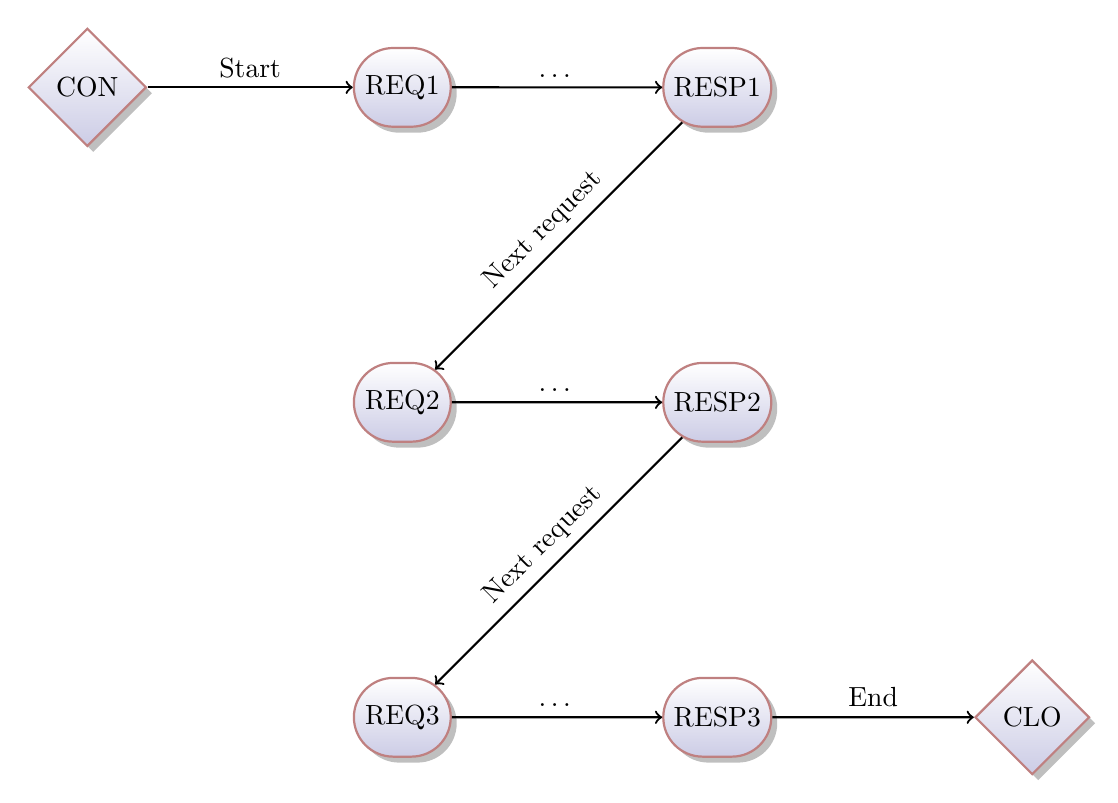
\begin{tikzpicture} [
    thick,
    node distance=4cm,
  ]
                     
  \tikzstyle{reqresp} = [
    rounded rectangle,
    thick,
 	 minimum size=1cm,
 	 draw=red!50!black!50,
 	 top color=white,
 	 bottom color=blue!50!black!20,
 	 drop shadow,
  ]
  \tikzstyle{conclo} = [
    reqresp,
    diamond,
  ]
	                    
  \node[conclo,diamond]        (con)   {CON};
  \node[reqresp,right of=con]   (req1)  {REQ1};
  \node[reqresp,right of=req1]  (resp1) {RESP1};
  \node[reqresp,below of=req1]  (req2)  {REQ2};
  \node[reqresp,right of=req2]  (resp2) {RESP2};

  \node[reqresp,below of=req2]  (req3)  {REQ3};
  \node[reqresp,right of=req3] (resp3) {RESP3};  
  
  \node[conclo,right of=resp3] (clo)   {CLO};
	
  \path[->] (con)   edge node[above] {Start}  (req1);
  \path[->] (req1)  edge node[above] {\ldots} (resp1);
  \path[->] (resp1) edge node[midway,sloped,above] {Next request} (req2);
  \path[->] (req2)  edge node[above] {\ldots} (resp2);
  \path[->] (resp2) edge node[midway,sloped,above] {Next request} (req3);
  \path[->] (req3)  edge node[above] {\ldots} (resp3);
  \path[->] (resp3) edge node[above] {End}    (clo);
	
  \end{tikzpicture}
  \caption{HTTP keep-alive mode}
  \label{fig:http_keep_alive}
\end{figure}

Its advantages are a reduced latency between transactions, and less processing
power required on the server side. It is generally better than the close mode,
but not always because the clients often limit their concurrent connections to
a smaller value.

A last improvement in the communications is the pipelining mode. It still uses
keep-alive, but the client does not wait for the first response to send the
second request. This is useful for fetching large number of images composing a
page. This mode is shown on Figure ~\ref{fig:http_pipelining}.

\begin{figure}[p]
  \centering
  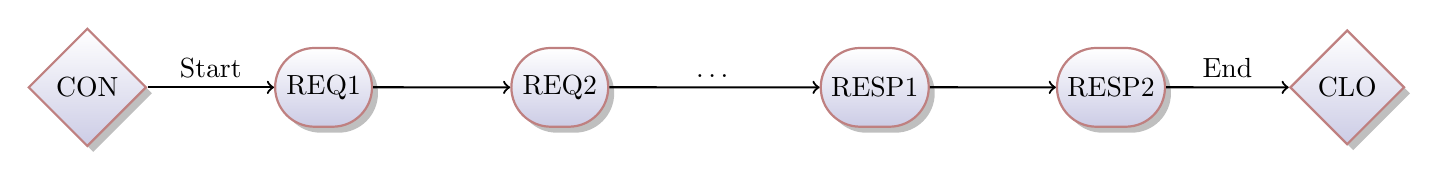
\begin{tikzpicture} [
    thick,
    node distance=3cm,
  ]
                     
  \tikzstyle{reqresp} = [
    rounded rectangle,
    thick,
 	 minimum size=1cm,
 	 draw=red!50!black!50,
 	 top color=white,
 	 bottom color=blue!50!black!20,
 	 drop shadow,
  ]
  \tikzstyle{conclo} = [
    reqresp,
    diamond,
  ]                    
	                    
  \node[conclo]                             (con)   {CON};
  \node[reqresp,right of=con]               (req1)  {REQ1};
  \node[reqresp,right of=req1]              (req2)  {REQ2};
  \node[reqresp,right of=req2, xshift=1cm]  (resp1) {RESP1};
  \node[reqresp,right of=resp1]             (resp2) {RESP2};
  \node[conclo,right of=resp2]              (clo)   {CLO};
	
  \path[->] (con)   edge node[above] {Start} (req1);
  \path[->] (req1)  edge (req2);
  \path[->] (req2)  edge node[above] {\ldots} (resp1);
  \path[->] (resp1) edge (resp2);
  \path[->] (resp2) edge node[above] {End} (clo);

  \end{tikzpicture}
  \caption{HTTP pipelining mode}
  \label{fig:http_pipelining}
\end{figure}

This can obviously have a tremendous benefit on performance because the network
latency is eliminated between subsequent requests. Many HTTP agents do not
correctly support pipelining since there is no way to associate a response with
the corresponding request in HTTP. For this reason, it is mandatory for the
server to reply in the exact same order as the requests were received.

By default HAProxy operates in a tunnel-like mode with regards to persistent
connections: for each connection it processes the first request and forwards
everything else (including additional requests) to selected server. Once
established, the connection is persisted both on the client and server
sides. Use "option http-server-close" to preserve client persistent connections
while handling every incoming request individually, dispatching them one after
another to servers, in HTTP close mode. Use "option httpclose" to switch both
sides to HTTP close mode. "option forceclose" and "option
http-pretend-keepalive" help working around servers misbehaving in HTTP close
mode.


\section{HTTP request}
First, let's consider this HTTP request:
\begin{verbatim}
  Line     Contents
  number
     1     GET /serv/login.php?lang=en&profile=2 HTTP/1.1
     2     Host: www.mydomain.com
     3     User-agent: my small browser
     4     Accept: image/jpeg, image/gif
     5     Accept: image/png
\end{verbatim}

\subsection{The Request line}
Line 1 is the "request line". It is always composed of 3 fields:

\begin{description}
  \item[METHOD:] GET
  \item[URI:] \verb|/serv/login.php?lang=en&profile=2|
  \item[version tag:] HTTP/1.1
\end{description}

All of them are delimited by what the standard calls LWS (linear white spaces),
which are commonly spaces, but can also be tabs or line feeds/carriage returns
followed by spaces/tabs. The method itself cannot contain any colon (':') and
is limited to alphabetic letters. All those various combinations make it
desirable that HAProxy performs the splitting itself rather than leaving it to
the user to write a complex or inaccurate regular expression.

The URI itself can have several forms:

\begin{description}
\item[A "relative URI"]
    It is a complete URL without the host part. This is generally what is
    received by servers, reverse proxies and transparent proxies.\\
    \verb|/serv/login.php?lang=en&profile=2|

\item[An "absolute URI", also called a "URL"]
    It is composed of a "scheme" (the protocol name followed by '://'), a host
    name or address, optionally a colon (':') followed by a port number, then
    a relative URI beginning at the first slash ('/') after the address part.
    This is generally what proxies receive, but a server supporting HTTP/1.1
    must accept this form too.\\
    \verb|http://192.168.0.12:8080/serv/login.php?lang=en&profile=2|

\item[A star "*"]
    This form is only accepted in association with the OPTIONS
    method and is not relayable. It is used to inquiry a next hop's
    capabilities.

\item[An address:port combination]
    This is used with the CONNECT method, which is used to establish TCP
    tunnels through HTTP proxies, generally for HTTPS, but sometimes for
    other protocols too.\\
    \verb|192.168.0.12:80|
\end{description}

In a relative URI, two sub-parts are identified. The part before the question
mark is called the "path". It is typically the relative path to static objects
on the server. The part after the question mark is called the "query string".
It is mostly used with GET requests sent to dynamic scripts and is very
specific to the language, framework or application in use.

\subsection{The request headers}
The headers start at the second line. They are composed of a name at the
beginning of the line, immediately followed by a colon (':'). Traditionally,
an LWS is added after the colon but that's not required. Then come the values.
Multiple identical headers may be folded into one single line, delimiting the
values with commas, provided that their order is respected. This is commonly
encountered in the "Cookie:" field. A header may span over multiple lines if
the subsequent lines begin with an LWS. In the example in 1.2, lines 4 and 5
define a total of 3 values for the "Accept:" header.

Contrary to a common mis-conception, header names are not case-sensitive, and
their values are not either if they refer to other header names (such as the
"Connection:" header).

The end of the headers is indicated by the first empty line. People often say
that it's a double line feed, which is not exact, even if a double line feed
is one valid form of empty line.

Fortunately, HAProxy takes care of all these complex combinations when indexing
headers, checking values and counting them, so there is no reason to worry
about the way they could be written, but it is important not to accuse an
application of being buggy if it does unusual, valid things.

\paragraph*{Important note:}
   As suggested by RFC2616, HAProxy normalizes headers by replacing line breaks
   in the middle of headers by LWS in order to join multi-line headers. This
   is necessary for proper analysis and helps less capable HTTP parsers to work
   correctly and not to be fooled by such complex constructs.


\section{HTTP response}
An HTTP response looks very much like an HTTP request. Both are called HTTP
messages. Let's consider this HTTP response:
\begin{enumerate}
   \item HTTP/1.1 200 OK
   \item Content-length: 350
   \item Content-Type: text/html
\end{enmerate}
As a special case, HTTP supports so called "Informational responses" as status
codes 1xx. These messages are special in that they don't convey any part of the
response, they're just used as sort of a signaling message to ask a client to
continue to post its request for instance. In the case of a status 100 response
the requested information will be carried by the next non-100 response message
following the informational one. This implies that multiple responses may be
sent to a single request, and that this only works when keep-alive is enabled
(1xx messages are HTTP/1.1 only). HAProxy handles these messages and is able to
correctly forward and skip them, and only process the next non-100 response. As
such, these messages are neither logged nor transformed, unless explicitly
state otherwise. Status 101 messages indicate that the protocol is changing
over the same connection and that haproxy must switch to tunnel mode, just as
if a CONNECT had occurred. Then the Upgrade header would contain additional
information about the type of protocol the connection is switching to.

\subsection{The Response line}
Line 1 is the "response line". It is always composed of 3 fields:

\begin{itemize}
  \item a version tag : HTTP/1.1
  \item a status code : 200
  \item a reason      : OK
\end{itemize}

The status code is always 3-digit. The first digit indicates a general status:

\begin{itemize}
  \item 1xx = informational message to be skipped (eg: 100, 101)
  \item 2xx = OK, content is following   (eg: 200, 206)
  \item 3xx = OK, no content following   (eg: 302, 304)
  \item 4xx = error caused by the client (eg: 401, 403, 404)
  \item 5xx = error caused by the server (eg: 500, 502, 503)
\end{itemize}

Please refer to RFC2616 for the detailed meaning of all such codes. The
"reason" field is just a hint, but is not parsed by clients. Anything can be
found there, but it's a common practice to respect the well-established
messages. It can be composed of one or multiple words, such as "OK", "Found",
or "Authentication Required".

Haproxy may emit the following status codes by itself:

\begin{description}
  \item[200] access to stats page, and when replying to monitoring requests
  \item[301] when performing a redirection, depending on the configured code
  \item[302] when performing a redirection, depending on the configured code
  \item[303] when performing a redirection, depending on the configured code
  \item[400] for an invalid or too large request
  \item[401] when an authentication is required to perform the action (when
        accessing the stats page)
  \item[403] when a request is forbidden by a "block" ACL or "reqdeny" filter
  \item[408] when the request timeout strikes before the request is complete
  \item[500] when haproxy encounters an unrecoverable internal error, such as a
        memory allocation failure, which should never happen
  \item[502] when the server returns an empty, invalid or incomplete response, or
        when an "rspdeny" filter blocks the response.
  \item[503] when no server was available to handle the request, or in response to
        monitoring requests which match the "monitor fail" condition
  \item[504] when the response timeout strikes before the server responds
\end{description}

The error 4xx and 5xx codes above may be customized (see "errorloc" in section
4.2).

\subsection{The response headers}
Response headers work exactly like request headers, and as such, HAProxy uses
the same parsing function for both. Please refer to paragraph 1.2.2 for more
details.

\chapter{Configuring HAProxy}
\section{Configuration file format}
HAProxy's configuration process involves 3 major sources of parameters:

\begin{enumerate}
  \item the arguments from the command-line, which always take precedence
  \item the "global" section, which sets process-wide parameters
  \item the proxies sections which can take form of "defaults", "listen",
    "frontend" and "backend".
\end{enumerate}

The configuration file syntax consists in lines beginning with a keyword
referenced in this manual, optionally followed by one or several parameters
delimited by spaces. If spaces have to be entered in strings, then they must be
preceded by a backslash ('\textbackslash') to be escaped. Backslashes also have to be
escaped by doubling them.

\section{Time format}
Some parameters involve values representing time, such as timeouts. These
values are generally expressed in milliseconds (unless explicitly stated
otherwise) but may be expressed in any other unit by suffixing the unit to the
numeric value. It is important to consider this because it will not be repeated
for every keyword. Supported units are:

\begin{description}
  \item[us:] microseconds. 1 microsecond = 1/1000000 second
  \item[ms:] milliseconds. 1 millisecond = 1/1000 second. This is the default.
  \item[s:]  seconds. 1s = 1000ms
  \item[m:]  minutes. 1m = 60s = 60000ms
  \item[h:]  hours.   1h = 60m = 3600s = 3600000ms
  \item[d:]  days.    1d = 24h = 1440m = 86400s = 86400000ms
\end{description}

\section{Examples}
\begin{verbatim}
    # Simple configuration for an HTTP proxy listening on port 80 on all
    # interfaces and forwarding requests to a single backend "servers" with a
    # single server "server1" listening on 127.0.0.1:8000
    global
        daemon
        maxconn 256

    defaults
        mode http
        timeout connect 5000ms
        timeout client 50000ms
        timeout server 50000ms

    frontend http-in
        bind *:80
        default_backend servers

    backend servers
        server server1 127.0.0.1:8000 maxconn 32


    # The same configuration defined with a single listen block. Shorter but
    # less expressive, especially in HTTP mode.
    global
        daemon
        maxconn 256

    defaults
        mode http
        timeout connect 5000ms
        timeout client 50000ms
        timeout server 50000ms

    listen http-in
        bind *:80
        server server1 127.0.0.1:8000 maxconn 32
\end{verbatim}

Assuming haproxy is in \$PATH, test these configurations in a shell with:

%\begin{verbatim}
%$ sudo haproxy -f configuration.conf -c
%\end{verbatim}

\chapter{Global parameters}
Parameters in the "global" section are process-wide and often OS-specific. They
are generally set once for all and do not need being changed once correct. Some
of them have command-line equivalents.

The following keywords are supported in the "global" section:

\begin{itemize}
\item Process management and security
  \begin{itemize}
    \item[-] chroot
    \item[-] daemon
    \item[-] gid
    \item[-] group
    \item[-] log
    \item[-] log-send-hostname
    \item[-] nbproc
    \item[-] pidfile
    \item[-] uid
    \item[-] ulimit-n
    \item[-] user
    \item[-] stats
    \item[-] node
    \item[-] description
    \item[-] unix-bind
  \end{itemize}
\item Performance tuning
  \begin{itemize}
    \item[-] maxconn
    \item[-] maxconnrate
    \item[-] maxpipes
    \item[-] noepoll
    \item[-] nokqueue
    \item[-] nopoll
    \item[-] nosepoll
    \item[-] nosplice
    \item[-] spread-checks
    \item[-] tune.bufsize
    \item[-] tune.chksize
    \item[-] tune.http.maxhdr
    \item[-] tune.maxaccept
    \item[-] tune.maxpollevents
    \item[-] tune.maxrewrite
    \item[-] tune.pipesize
    \item[-] tune.rcvbuf.client
    \item[-] tune.rcvbuf.server
    \item[-] tune.sndbuf.client
    \item[-] tune.sndbuf.server
  \end{itemize}
\item Debugging
  \begin{itemize}
    \item[-] debug
    \item[-] quiet
  \end{itemize}
\end{itemize}

\section{Process management and security}

\begin{description}
\item[chroot <jail dir>]
  Changes current directory to <jail dir> and performs a chroot() there before
  dropping privileges. This increases the security level in case an unknown
  vulnerability would be exploited, since it would make it very hard for the
  attacker to exploit the system. This only works when the process is started
  with superuser privileges. It is important to ensure that <jail\_dir> is both
  empty and unwritable to anyone.
\item[daemon]
  Makes the process fork into background. This is the recommended mode of
  operation. It is equivalent to the command line "-D" argument. It can be
  disabled by the command line "-db" argument.
\item[gid <number>]
  Changes the process' group ID to <number>. It is recommended that the group
  ID is dedicated to HAProxy or to a small set of similar daemons. HAProxy must
  be started with a user belonging to this group, or with superuser privileges.
  See also "group" and "uid".
\item[group <group name>]
  Similar to "gid" but uses the GID of group name <group name> from /etc/group.
  See also "gid" and "user".
\item[{log <address> <facility> [max level [min level]]}]
  Adds a global syslog server. Up to two global servers can be defined. They
  will receive logs for startups and exits, as well as all logs from proxies
  configured with "log global".

  <address> can be one of:
  
  \begin{itemize}
    \item[-] An IPv4 address optionally followed by a colon and a UDP port. If
          no port is specified, 514 is used by default (the standard syslog
          port).

    \item[-] An IPv6 address followed by a colon and optionally a UDP port. If
          no port is specified, 514 is used by default (the standard syslog
          port).

    \item[-] A filesystem path to a UNIX domain socket, keeping in mind
          considerations for chroot (be sure the path is accessible inside
          the chroot) and uid/gid (be sure the path is appropriately
          writeable).
  \end{itemize}
  
  <facility> must be one of the 24 standard syslog facilities:
  
  \begin{verbatim}
          kern   user   mail   daemon auth   syslog lpr    news
          uucp   cron   auth2  ftp    ntp    audit  alert  cron2
          local0 local1 local2 local3 local4 local5 local6 local7
  \end{verbatim}
  
  An optional level can be specified to filter outgoing messages. By default,
  all messages are sent. If a maximum level is specified, only messages with a
  severity at least as important as this level will be sent. An optional minimum
  level can be specified. If it is set, logs emitted with a more severe level
  than this one will be capped to this level. This is used to avoid sending
  "emerg" messages on all terminals on some default syslog configurations.
  
  Eight levels are known:
  
  \begin{verbatim}
          emerg  alert  crit   err    warning notice info  debug
  \end{verbatim}
  
\item[{log-send-hostname [<string>]}]
  Sets the hostname field in the syslog header. If optional "string" parameter
  is set the header is set to the string contents, otherwise uses the hostname
  of the system. Generally used if one is not relaying logs through an
  intermediate syslog server or for simply customizing the hostname printed in
  the logs.

\item[log-tag <string>]
  Sets the tag field in the syslog header to this string. It defaults to the
  program name as launched from the command line, which usually is "haproxy".
  Sometimes it can be useful to differentiate between multiple processes
  running on the same host.

\item[nbproc <number>]
  Creates <number> processes when going daemon. This requires the "daemon"
  mode. By default, only one process is created, which is the recommended mode
  of operation. For systems limited to small sets of file descriptors per
  process, it may be needed to fork multiple daemons. USING MULTIPLE PROCESSES
  IS HARDER TO DEBUG AND IS REALLY DISCOURAGED. See also "daemon".

\item[pidfile <pidfile>]
  Writes pids of all daemons into file <pidfile>. This option is equivalent to
  the "-p" command line argument. The file must be accessible to the user
  starting the process. See also "daemon".
  
  \begin{verbatim}
  stats socket <path> [{uid | user} <uid>] [{gid | group} <gid>] [mode <mode>]
             [level <level>]
  \end{verbatim}

  Creates a UNIX socket in stream mode at location <path>. Any previously
  existing socket will be backed up then replaced. Connections to this socket
  will return various statistics outputs and even allow some commands to be
  issued. Please consult section 9.2 "Unix Socket commands" for more details.
  
  An optional "level" parameter can be specified to restrict the nature of
  the commands that can be issued on the socket:
  \begin{itemize}
    \item[-] "user" is the least privileged level; only non-sensitive stats can be
      read, and no change is allowed. It would make sense on systems where it
      is not easy to restrict access to the socket.

    \item[-] "operator" is the default level and fits most common uses. All data can
      be read, and only non-sensitive changes are permitted (eg: clear max
      counters).

    \item[-] "admin" should be used with care, as everything is permitted (eg: clear
      all counters).
  \end{itemize}
  On platforms which support it, it is possible to restrict access to this
  socket by specifying numerical IDs after "uid" and "gid", or valid user and
  group names after the "user" and "group" keywords. It is also possible to
  restrict permissions on the socket by passing an octal value after the "mode"
  keyword (same syntax as chmod). Depending on the platform, the permissions on
  the socket will be inherited from the directory which hosts it, or from the
  user the process is started with.

\item[stats timeout <timeout, in milliseconds>]
  The default timeout on the stats socket is set to 10 seconds. It is possible
  to change this value with "stats timeout". The value must be passed in
  milliseconds, or be suffixed by a time unit among { us, ms, s, m, h, d }.

\item[stats maxconn <connections>]
  By default, the stats socket is limited to 10 concurrent connections. It is
  possible to change this value with "stats maxconn".

\item[uid <number>]
  Changes the process' user ID to <number>. It is recommended that the user ID
  is dedicated to HAProxy or to a small set of similar daemons. HAProxy must
  be started with superuser privileges in order to be able to switch to another
  one. See also "gid" and "user".

\item[ulimit-n <number>]
  Sets the maximum number of per-process file-descriptors to <number>. By
  default, it is automatically computed, so it is recommended not to use this
  option.

\item [unix-bind]
  \begin{verbatim}
  [ prefix <prefix> ] [ mode <mode> ]
  [ user <user> ] [ uid <uid> ]
  [ group <group> ] [ gid <gid> ]
  \end{verbatim}

  Fixes common settings to UNIX listening sockets declared in "bind" statements.
  This is mainly used to simplify declaration of those UNIX sockets and reduce
  the risk of errors, since those settings are most commonly required but are
  also process-specific. The <prefix> setting can be used to force all socket
  path to be relative to that directory. This might be needed to access another
  component's chroot. Note that those paths are resolved before haproxy chroots
  itself, so they are absolute. The <mode>, <user>, <uid>, <group> and <gid>
  all have the same meaning as their homonyms used by the "bind" statement. If
  both are specified, the "bind" statement has priority, meaning that the
  "unix-bind" settings may be seen as process-wide default settings.

\item[user <user name>]
  Similar to "uid" but uses the UID of user name <user name> from /etc/passwd.
  See also "uid" and "group".

\item[node <name>]
  Only letters, digits, hyphen and underscore are allowed, like in DNS names.

  This statement is useful in HA configurations where two or more processes or
  servers share the same IP address. By setting a different node-name on all
  nodes, it becomes easy to immediately spot what server is handling the
  traffic.

\item[description <text>]
  Add a text that describes the instance.

  Please note that it is required to escape certain characters (# for example)
  and this text is inserted into a html page so you should avoid using
  "<" and ">" characters.
\end{description}

\begin{comment}

3.2. Performance tuning
-----------------------

maxconn <number>
  Sets the maximum per-process number of concurrent connections to <number>. It
  is equivalent to the command-line argument "-n". Proxies will stop accepting
  connections when this limit is reached. The "ulimit-n" parameter is
  automatically adjusted according to this value. See also "ulimit-n".

maxconnrate <number>
  Sets the maximum per-process number of connections per second to <number>.
  Proxies will stop accepting connections when this limit is reached. It can be
  used to limit the global capacity regardless of each frontend capacity. It is
  important to note that this can only be used as a service protection measure,
  as there will not necessarily be a fair share between frontends when the
  limit is reached, so it's a good idea to also limit each frontend to some
  value close to its expected share. Also, lowering tune.maxaccept can improve
  fairness.

maxpipes <number>
  Sets the maximum per-process number of pipes to <number>. Currently, pipes
  are only used by kernel-based tcp splicing. Since a pipe contains two file
  descriptors, the "ulimit-n" value will be increased accordingly. The default
  value is maxconn/4, which seems to be more than enough for most heavy usages.
  The splice code dynamically allocates and releases pipes, and can fall back
  to standard copy, so setting this value too low may only impact performance.

noepoll
  Disables the use of the "epoll" event polling system on Linux. It is
  equivalent to the command-line argument "-de". The next polling system
  used will generally be "poll". See also "nosepoll", and "nopoll".

nokqueue
  Disables the use of the "kqueue" event polling system on BSD. It is
  equivalent to the command-line argument "-dk". The next polling system
  used will generally be "poll". See also "nopoll".

nopoll
  Disables the use of the "poll" event polling system. It is equivalent to the
  command-line argument "-dp". The next polling system used will be "select".
  It should never be needed to disable "poll" since it's available on all
  platforms supported by HAProxy. See also "nosepoll", and "nopoll" and
  "nokqueue".

nosepoll
  Disables the use of the "speculative epoll" event polling system on Linux. It
  is equivalent to the command-line argument "-ds". The next polling system
  used will generally be "epoll". See also "nosepoll", and "nopoll".

nosplice
  Disables the use of kernel tcp splicing between sockets on Linux. It is
  equivalent to the command line argument "-dS".  Data will then be copied
  using conventional and more portable recv/send calls. Kernel tcp splicing is
  limited to some very recent instances of kernel 2.6. Most versions between
  2.6.25 and 2.6.28 are buggy and will forward corrupted data, so they must not
  be used. This option makes it easier to globally disable kernel splicing in
  case of doubt. See also "option splice-auto", "option splice-request" and
  "option splice-response".

spread-checks <0..50, in percent>
  Sometimes it is desirable to avoid sending health checks to servers at exact
  intervals, for instance when many logical servers are located on the same
  physical server. With the help of this parameter, it becomes possible to add
  some randomness in the check interval between 0 and +/- 50%. A value between
  2 and 5 seems to show good results. The default value remains at 0.

tune.bufsize <number>
  Sets the buffer size to this size (in bytes). Lower values allow more
  sessions to coexist in the same amount of RAM, and higher values allow some
  applications with very large cookies to work. The default value is 16384 and
  can be changed at build time. It is strongly recommended not to change this
  from the default value, as very low values will break some services such as
  statistics, and values larger than default size will increase memory usage,
  possibly causing the system to run out of memory. At least the global maxconn
  parameter should be decreased by the same factor as this one is increased.

tune.chksize <number>
  Sets the check buffer size to this size (in bytes). Higher values may help
  find string or regex patterns in very large pages, though doing so may imply
  more memory and CPU usage. The default value is 16384 and can be changed at
  build time. It is not recommended to change this value, but to use better
  checks whenever possible.

tune.http.maxhdr <number>
  Sets the maximum number of headers in a request. When a request comes with a
  number of headers greater than this value (including the first line), it is
  rejected with a "400 Bad Request" status code. Similarly, too large responses
  are blocked with "502 Bad Gateway". The default value is 101, which is enough
  for all usages, considering that the widely deployed Apache server uses the
  same limit. It can be useful to push this limit further to temporarily allow
  a buggy application to work by the time it gets fixed. Keep in mind that each
  new header consumes 32bits of memory for each session, so don't push this
  limit too high.

tune.maxaccept <number>
  Sets the maximum number of consecutive accepts that a process may perform on
  a single wake up. High values give higher priority to high connection rates,
  while lower values give higher priority to already established connections.
  This value is limited to 100 by default in single process mode. However, in
  multi-process mode (nbproc > 1), it defaults to 8 so that when one process
  wakes up, it does not take all incoming connections for itself and leaves a
  part of them to other processes. Setting this value to -1 completely disables
  the limitation. It should normally not be needed to tweak this value.

tune.maxpollevents <number>
  Sets the maximum amount of events that can be processed at once in a call to
  the polling system. The default value is adapted to the operating system. It
  has been noticed that reducing it below 200 tends to slightly decrease
  latency at the expense of network bandwidth, and increasing it above 200
  tends to trade latency for slightly increased bandwidth.

tune.maxrewrite <number>
  Sets the reserved buffer space to this size in bytes. The reserved space is
  used for header rewriting or appending. The first reads on sockets will never
  fill more than bufsize-maxrewrite. Historically it has defaulted to half of
  bufsize, though that does not make much sense since there are rarely large
  numbers of headers to add. Setting it too high prevents processing of large
  requests or responses. Setting it too low prevents addition of new headers
  to already large requests or to POST requests. It is generally wise to set it
  to about 1024. It is automatically readjusted to half of bufsize if it is
  larger than that. This means you don't have to worry about it when changing
  bufsize.

tune.pipesize <number>
  Sets the kernel pipe buffer size to this size (in bytes). By default, pipes
  are the default size for the system. But sometimes when using TCP splicing,
  it can improve performance to increase pipe sizes, especially if it is
  suspected that pipes are not filled and that many calls to splice() are
  performed. This has an impact on the kernel's memory footprint, so this must
  not be changed if impacts are not understood.

tune.rcvbuf.client <number>
tune.rcvbuf.server <number>
  Forces the kernel socket receive buffer size on the client or the server side
  to the specified value in bytes. This value applies to all TCP/HTTP frontends
  and backends. It should normally never be set, and the default size (0) lets
  the kernel autotune this value depending on the amount of available memory.
  However it can sometimes help to set it to very low values (eg: 4096) in
  order to save kernel memory by preventing it from buffering too large amounts
  of received data. Lower values will significantly increase CPU usage though.

tune.sndbuf.client <number>
tune.sndbuf.server <number>
  Forces the kernel socket send buffer size on the client or the server side to
  the specified value in bytes. This value applies to all TCP/HTTP frontends
  and backends. It should normally never be set, and the default size (0) lets
  the kernel autotune this value depending on the amount of available memory.
  However it can sometimes help to set it to very low values (eg: 4096) in
  order to save kernel memory by preventing it from buffering too large amounts
  of received data. Lower values will significantly increase CPU usage though.
  Another use case is to prevent write timeouts with extremely slow clients due
  to the kernel waiting for a large part of the buffer to be read before
  notifying haproxy again.


3.3. Debugging
--------------

debug
  Enables debug mode which dumps to stdout all exchanges, and disables forking
  into background. It is the equivalent of the command-line argument "-d". It
  should never be used in a production configuration since it may prevent full
  system startup.

quiet
  Do not display any message during startup. It is equivalent to the command-
  line argument "-q".


3.4. Userlists
--------------
It is possible to control access to frontend/backend/listen sections or to
http stats by allowing only authenticated and authorized users. To do this,
it is required to create at least one userlist and to define users.

userlist <listname>
  Creates new userlist with name <listname>. Many independent userlists can be
  used to store authentication & authorization data for independent customers.

group <groupname> [users <user>,<user>,(...)]
  Adds group <groupname> to the current userlist. It is also possible to
  attach users to this group by using a comma separated list of names
  proceeded by "users" keyword.

user <username> [password|insecure-password <password>]
                [groups <group>,<group>,(...)]
  Adds user <username> to the current userlist. Both secure (encrypted) and
  insecure (unencrypted) passwords can be used. Encrypted passwords are
  evaluated using the crypt(3) function so depending of the system's
  capabilities, different algorithms are supported. For example modern Glibc
  based Linux system supports MD5, SHA-256, SHA-512 and of course classic,
  DES-based method of crypting passwords.


  Example:
        userlist L1
          group G1 users tiger,scott
          group G2 users xdb,scott

          user tiger password $6$k6y3o.eP$JlKBx9za9667qe4(...)xHSwRv6J.C0/D7cV91
          user scott insecure-password elgato
          user xdb insecure-password hello

        userlist L2
          group G1
          group G2

          user tiger password $6$k6y3o.eP$JlKBx(...)xHSwRv6J.C0/D7cV91 groups G1
          user scott insecure-password elgato groups G1,G2
          user xdb insecure-password hello groups G2

  Please note that both lists are functionally identical.


3.5. Peers
----------
It is possible to synchronize server entries in stick tables between several
haproxy instances over TCP connections in a multi-master fashion. Each instance
pushes its local updates and insertions to remote peers. Server IDs are used to
identify servers remotely, so it is important that configurations look similar
or at least that the same IDs are forced on each server on all participants.
Interrupted exchanges are automatically detected and recovered from the last
known point. In addition, during a soft restart, the old process connects to
the new one using such a TCP connection to push all its entries before the new
process tries to connect to other peers. That ensures very fast replication
during a reload, it typically takes a fraction of a second even for large
tables.

peers <peersect>
  Creates a new peer list with name <peersect>. It is an independant section,
  which is referenced by one or more stick-tables.

peer <peername> <ip>:<port>
  Defines a peer inside a peers section.
  If <peername> is set to the local peer name (by default hostname, or forced
  using "-L" command line option), haproxy will listen for incoming remote peer
  connection on <ip>:<port>. Otherwise, <ip>:<port> defines where to connect to
  to join the remote peer, and <peername> is used at the protocol level to
  identify and validate the remote peer on the server side.

  During a soft restart, local peer <ip>:<port> is used by the old instance to
  connect the new one and initiate a complete replication (teaching process).

  It is strongly recommended to have the exact same peers declaration on all
  peers and to only rely on the "-L" command line argument to change the local
  peer name. This makes it easier to maintain coherent configuration files
  across all peers.

  Example:
    peers mypeers
        peer haproxy1 192.168.0.1:1024
        peer haproxy2 192.168.0.2:1024
        peer haproxy3 10.2.0.1:1024

    backend mybackend
        mode tcp
        balance roundrobin
        stick-table type ip size 20k peers mypeers
        stick on src

        server srv1 192.168.0.30:80
        server srv2 192.168.0.31:80


4. Proxies
----------

Proxy configuration can be located in a set of sections :
 - defaults <name>
 - frontend <name>
 - backend  <name>
 - listen   <name>

A "defaults" section sets default parameters for all other sections following
its declaration. Those default parameters are reset by the next "defaults"
section. See below for the list of parameters which can be set in a "defaults"
section. The name is optional but its use is encouraged for better readability.

A "frontend" section describes a set of listening sockets accepting client
connections.

A "backend" section describes a set of servers to which the proxy will connect
to forward incoming connections.

A "listen" section defines a complete proxy with its frontend and backend
parts combined in one section. It is generally useful for TCP-only traffic.

All proxy names must be formed from upper and lower case letters, digits,
'-' (dash), '_' (underscore) , '.' (dot) and ':' (colon). ACL names are
case-sensitive, which means that "www" and "WWW" are two different proxies.

Historically, all proxy names could overlap, it just caused troubles in the
logs. Since the introduction of content switching, it is mandatory that two
proxies with overlapping capabilities (frontend/backend) have different names.
However, it is still permitted that a frontend and a backend share the same
name, as this configuration seems to be commonly encountered.

Right now, two major proxy modes are supported : "tcp", also known as layer 4,
and "http", also known as layer 7. In layer 4 mode, HAProxy simply forwards
bidirectional traffic between two sides. In layer 7 mode, HAProxy analyzes the
protocol, and can interact with it by allowing, blocking, switching, adding,
modifying, or removing arbitrary contents in requests or responses, based on
arbitrary criteria.


4.1. Proxy keywords matrix
--------------------------

The following list of keywords is supported. Most of them may only be used in a
limited set of section types. Some of them are marked as "deprecated" because
they are inherited from an old syntax which may be confusing or functionally
limited, and there are new recommended keywords to replace them. Keywords
marked with "(*)" can be optionally inverted using the "no" prefix, eg. "no
option contstats". This makes sense when the option has been enabled by default
and must be disabled for a specific instance. Such options may also be prefixed
with "default" in order to restore default settings regardless of what has been
specified in a previous "defaults" section.


 keyword                              defaults   frontend   listen    backend
------------------------------------+----------+----------+---------+---------
acl                                       -          X         X         X
appsession                                -          -         X         X
backlog                                   X          X         X         -
balance                                   X          -         X         X
bind                                      -          X         X         -
bind-process                              X          X         X         X
block                                     -          X         X         X
capture cookie                            -          X         X         -
capture request header                    -          X         X         -
capture response header                   -          X         X         -
clitimeout                  (deprecated)  X          X         X         -
contimeout                  (deprecated)  X          -         X         X
cookie                                    X          -         X         X
default-server                            X          -         X         X
default_backend                           X          X         X         -
description                               -          X         X         X
disabled                                  X          X         X         X
dispatch                                  -          -         X         X
enabled                                   X          X         X         X
errorfile                                 X          X         X         X
errorloc                                  X          X         X         X
errorloc302                               X          X         X         X
-- keyword -------------------------- defaults - frontend - listen -- backend -
errorloc303                               X          X         X         X
force-persist                             -          X         X         X
fullconn                                  X          -         X         X
grace                                     X          X         X         X
hash-type                                 X          -         X         X
http-check disable-on-404                 X          -         X         X
http-check expect                         -          -         X         X
http-check send-state                     X          -         X         X
http-request                              -          X         X         X
id                                        -          X         X         X
ignore-persist                            -          X         X         X
log                                  (*)  X          X         X         X
maxconn                                   X          X         X         -
mode                                      X          X         X         X
monitor fail                              -          X         X         -
monitor-net                               X          X         X         -
monitor-uri                               X          X         X         -
option abortonclose                  (*)  X          -         X         X
option accept-invalid-http-request   (*)  X          X         X         -
option accept-invalid-http-response  (*)  X          -         X         X
option allbackups                    (*)  X          -         X         X
option checkcache                    (*)  X          -         X         X
option clitcpka                      (*)  X          X         X         -
option contstats                     (*)  X          X         X         -
option dontlog-normal                (*)  X          X         X         -
option dontlognull                   (*)  X          X         X         -
option forceclose                    (*)  X          X         X         X
-- keyword -------------------------- defaults - frontend - listen -- backend -
option forwardfor                         X          X         X         X
option http-no-delay                 (*)  X          X         X         X
option http-pretend-keepalive        (*)  X          X         X         X
option http-server-close             (*)  X          X         X         X
option http-use-proxy-header         (*)  X          X         X         -
option httpchk                            X          -         X         X
option httpclose                     (*)  X          X         X         X
option httplog                            X          X         X         X
option http_proxy                    (*)  X          X         X         X
option independant-streams           (*)  X          X         X         X
option ldap-check                         X          -         X         X
option log-health-checks             (*)  X          -         X         X
option log-separate-errors           (*)  X          X         X         -
option logasap                       (*)  X          X         X         -
option mysql-check                        X          -         X         X
option pgsql-check                        X          -         X         X
option nolinger                      (*)  X          X         X         X
option originalto                         X          X         X         X
option persist                       (*)  X          -         X         X
option redispatch                    (*)  X          -         X         X
option redis-check                        X          -         X         X
option smtpchk                            X          -         X         X
option socket-stats                  (*)  X          X         X         -
option splice-auto                   (*)  X          X         X         X
option splice-request                (*)  X          X         X         X
option splice-response               (*)  X          X         X         X
option srvtcpka                      (*)  X          -         X         X
option ssl-hello-chk                      X          -         X         X
-- keyword -------------------------- defaults - frontend - listen -- backend -
option tcp-smart-accept              (*)  X          X         X         -
option tcp-smart-connect             (*)  X          -         X         X
option tcpka                              X          X         X         X
option tcplog                             X          X         X         X
option transparent                   (*)  X          -         X         X
persist rdp-cookie                        X          -         X         X
rate-limit sessions                       X          X         X         -
redirect                                  -          X         X         X
redisp                      (deprecated)  X          -         X         X
redispatch                  (deprecated)  X          -         X         X
reqadd                                    -          X         X         X
reqallow                                  -          X         X         X
reqdel                                    -          X         X         X
reqdeny                                   -          X         X         X
reqiallow                                 -          X         X         X
reqidel                                   -          X         X         X
reqideny                                  -          X         X         X
reqipass                                  -          X         X         X
reqirep                                   -          X         X         X
reqisetbe                                 -          X         X         X
reqitarpit                                -          X         X         X
reqpass                                   -          X         X         X
reqrep                                    -          X         X         X
-- keyword -------------------------- defaults - frontend - listen -- backend -
reqsetbe                                  -          X         X         X
reqtarpit                                 -          X         X         X
retries                                   X          -         X         X
rspadd                                    -          X         X         X
rspdel                                    -          X         X         X
rspdeny                                   -          X         X         X
rspidel                                   -          X         X         X
rspideny                                  -          X         X         X
rspirep                                   -          X         X         X
rsprep                                    -          X         X         X
server                                    -          -         X         X
source                                    X          -         X         X
srvtimeout                  (deprecated)  X          -         X         X
stats admin                               -          -         X         X
stats auth                                X          -         X         X
stats enable                              X          -         X         X
stats hide-version                        X          -         X         X
stats http-request                        -          -         X         X
stats realm                               X          -         X         X
stats refresh                             X          -         X         X
stats scope                               X          -         X         X
stats show-desc                           X          -         X         X
stats show-legends                        X          -         X         X
stats show-node                           X          -         X         X
stats uri                                 X          -         X         X
-- keyword -------------------------- defaults - frontend - listen -- backend -
stick match                               -          -         X         X
stick on                                  -          -         X         X
stick store-request                       -          -         X         X
stick store-response                      -          -         X         X
stick-table                               -          -         X         X
tcp-request connection                    -          X         X         -
tcp-request content                       -          X         X         X
tcp-request inspect-delay                 -          X         X         X
tcp-response content                      -          -         X         X
tcp-response inspect-delay                -          -         X         X
timeout check                             X          -         X         X
timeout client                            X          X         X         -
timeout clitimeout          (deprecated)  X          X         X         -
timeout connect                           X          -         X         X
timeout contimeout          (deprecated)  X          -         X         X
timeout http-keep-alive                   X          X         X         X
timeout http-request                      X          X         X         X
timeout queue                             X          -         X         X
timeout server                            X          -         X         X
timeout srvtimeout          (deprecated)  X          -         X         X
timeout tarpit                            X          X         X         X
timeout tunnel                            X          -         X         X
transparent                 (deprecated)  X          -         X         X
unique-id-format                          X          X         X         -
unique-id-header                          X          X         X         -
use_backend                               -          X         X         -
use-server                                -          -         X         X
------------------------------------+----------+----------+---------+---------
 keyword                              defaults   frontend   listen    backend


4.2. Alphabetically sorted keywords reference
---------------------------------------------

This section provides a description of each keyword and its usage.


acl <aclname> <criterion> [flags] [operator] <value> ...
  Declare or complete an access list.
  May be used in sections :   defaults | frontend | listen | backend
                                 no    |    yes   |   yes  |   yes
  Example:
        acl invalid_src  src          0.0.0.0/7 224.0.0.0/3
        acl invalid_src  src_port     0:1023
        acl local_dst    hdr(host) -i localhost

  See section 7 about ACL usage.


appsession <cookie> len <length> timeout <holdtime>
           [request-learn] [prefix] [mode <path-parameters|query-string>]
  Define session stickiness on an existing application cookie.
  May be used in sections :   defaults | frontend | listen | backend
                                 no    |    no    |   yes  |   yes
  Arguments :
    <cookie>   this is the name of the cookie used by the application and which
               HAProxy will have to learn for each new session.

    <length>   this is the max number of characters that will be memorized and
               checked in each cookie value.

    <holdtime> this is the time after which the cookie will be removed from
               memory if unused. If no unit is specified, this time is in
               milliseconds.

    request-learn
               If this option is specified, then haproxy will be able to learn
               the cookie found in the request in case the server does not
               specify any in response. This is typically what happens with
               PHPSESSID cookies, or when haproxy's session expires before
               the application's session and the correct server is selected.
               It is recommended to specify this option to improve reliability.

    prefix     When this option is specified, haproxy will match on the cookie
               prefix (or URL parameter prefix). The appsession value is the
               data following this prefix.

               Example :
               appsession ASPSESSIONID len 64 timeout 3h prefix

               This will match the cookie ASPSESSIONIDXXXX=XXXXX,
               the appsession value will be XXXX=XXXXX.

    mode       This option allows to change the URL parser mode.
               2 modes are currently supported :
               - path-parameters :
                 The parser looks for the appsession in the path parameters
                 part (each parameter is separated by a semi-colon), which is
                 convenient for JSESSIONID for example.
                 This is the default mode if the option is not set.
               - query-string :
                 In this mode, the parser will look for the appsession in the
                 query string.

  When an application cookie is defined in a backend, HAProxy will check when
  the server sets such a cookie, and will store its value in a table, and
  associate it with the server's identifier. Up to <length> characters from
  the value will be retained. On each connection, haproxy will look for this
  cookie both in the "Cookie:" headers, and as a URL parameter (depending on
  the mode used). If a known value is found, the client will be directed to the
  server associated with this value. Otherwise, the load balancing algorithm is
  applied. Cookies are automatically removed from memory when they have been
  unused for a duration longer than <holdtime>.

  The definition of an application cookie is limited to one per backend.

  Note : Consider not using this feature in multi-process mode (nbproc > 1)
         unless you know what you do : memory is not shared between the
         processes, which can result in random behaviours.

  Example :
        appsession JSESSIONID len 52 timeout 3h

  See also : "cookie", "capture cookie", "balance", "stick", "stick-table",
             "ignore-persist", "nbproc" and "bind-process".


backlog <conns>
  Give hints to the system about the approximate listen backlog desired size
  May be used in sections :   defaults | frontend | listen | backend
                                 yes   |    yes   |   yes  |   no
  Arguments :
    <conns>   is the number of pending connections. Depending on the operating
              system, it may represent the number of already acknowledged
              connections, of non-acknowledged ones, or both.

  In order to protect against SYN flood attacks, one solution is to increase
  the system's SYN backlog size. Depending on the system, sometimes it is just
  tunable via a system parameter, sometimes it is not adjustable at all, and
  sometimes the system relies on hints given by the application at the time of
  the listen() syscall. By default, HAProxy passes the frontend's maxconn value
  to the listen() syscall. On systems which can make use of this value, it can
  sometimes be useful to be able to specify a different value, hence this
  backlog parameter.

  On Linux 2.4, the parameter is ignored by the system. On Linux 2.6, it is
  used as a hint and the system accepts up to the smallest greater power of
  two, and never more than some limits (usually 32768).

  See also : "maxconn" and the target operating system's tuning guide.


balance <algorithm> [ <arguments> ]
balance url_param <param> [check_post [<max_wait>]]
  Define the load balancing algorithm to be used in a backend.
  May be used in sections :   defaults | frontend | listen | backend
                                 yes   |    no    |   yes  |   yes
  Arguments :
    <algorithm> is the algorithm used to select a server when doing load
                balancing. This only applies when no persistence information
                is available, or when a connection is redispatched to another
                server. <algorithm> may be one of the following :

      roundrobin  Each server is used in turns, according to their weights.
                  This is the smoothest and fairest algorithm when the server's
                  processing time remains equally distributed. This algorithm
                  is dynamic, which means that server weights may be adjusted
                  on the fly for slow starts for instance. It is limited by
                  design to 4128 active servers per backend. Note that in some
                  large farms, when a server becomes up after having been down
                  for a very short time, it may sometimes take a few hundreds
                  requests for it to be re-integrated into the farm and start
                  receiving traffic. This is normal, though very rare. It is
                  indicated here in case you would have the chance to observe
                  it, so that you don't worry.

      static-rr   Each server is used in turns, according to their weights.
                  This algorithm is as similar to roundrobin except that it is
                  static, which means that changing a server's weight on the
                  fly will have no effect. On the other hand, it has no design
                  limitation on the number of servers, and when a server goes
                  up, it is always immediately reintroduced into the farm, once
                  the full map is recomputed. It also uses slightly less CPU to
                  run (around -1%).

      leastconn   The server with the lowest number of connections receives the
                  connection. Round-robin is performed within groups of servers
                  of the same load to ensure that all servers will be used. Use
                  of this algorithm is recommended where very long sessions are
                  expected, such as LDAP, SQL, TSE, etc... but is not very well
                  suited for protocols using short sessions such as HTTP. This
                  algorithm is dynamic, which means that server weights may be
                  adjusted on the fly for slow starts for instance.

      first       The first server with available connection slots receives the
                  connection. The servers are choosen from the lowest numeric
                  identifier to the highest (see server parameter "id"), which
                  defaults to the server's position in the farm. Once a server
                  reaches its maxconn value, the next server is used. It does
                  not make sense to use this algorithm without setting maxconn.
                  The purpose of this algorithm is to always use the smallest
                  number of servers so that extra servers can be powered off
                  during non-intensive hours. This algorithm ignores the server
                  weight, and brings more benefit to long session such as RDP
                  or IMAP than HTTP, though it can be useful there too. In
                  order to use this algorithm efficiently, it is recommended
                  that a cloud controller regularly checks server usage to turn
                  them off when unused, and regularly checks backend queue to
                  turn new servers on when the queue inflates. Alternatively,
                  using "http-check send-state" may inform servers on the load.

      source      The source IP address is hashed and divided by the total
                  weight of the running servers to designate which server will
                  receive the request. This ensures that the same client IP
                  address will always reach the same server as long as no
                  server goes down or up. If the hash result changes due to the
                  number of running servers changing, many clients will be
                  directed to a different server. This algorithm is generally
                  used in TCP mode where no cookie may be inserted. It may also
                  be used on the Internet to provide a best-effort stickiness
                  to clients which refuse session cookies. This algorithm is
                  static by default, which means that changing a server's
                  weight on the fly will have no effect, but this can be
                  changed using "hash-type".

      uri         This algorithm hashes either the left part of the URI (before
                  the question mark) or the whole URI (if the "whole" parameter
                  is present) and divides the hash value by the total weight of
                  the running servers. The result designates which server will
                  receive the request. This ensures that the same URI will
                  always be directed to the same server as long as no server
                  goes up or down. This is used with proxy caches and
                  anti-virus proxies in order to maximize the cache hit rate.
                  Note that this algorithm may only be used in an HTTP backend.
                  This algorithm is static by default, which means that
                  changing a server's weight on the fly will have no effect,
                  but this can be changed using "hash-type".

                  This algorithm supports two optional parameters "len" and
                  "depth", both followed by a positive integer number. These
                  options may be helpful when it is needed to balance servers
                  based on the beginning of the URI only. The "len" parameter
                  indicates that the algorithm should only consider that many
                  characters at the beginning of the URI to compute the hash.
                  Note that having "len" set to 1 rarely makes sense since most
                  URIs start with a leading "/".

                  The "depth" parameter indicates the maximum directory depth
                  to be used to compute the hash. One level is counted for each
                  slash in the request. If both parameters are specified, the
                  evaluation stops when either is reached.

      url_param   The URL parameter specified in argument will be looked up in
                  the query string of each HTTP GET request.

                  If the modifier "check_post" is used, then an HTTP POST
                  request entity will be searched for the parameter argument,
                  when it is not found in a query string after a question mark
                  ('?') in the URL. Optionally, specify a number of octets to
                  wait for before attempting to search the message body. If the
                  entity can not be searched, then round robin is used for each
                  request. For instance, if your clients always send the LB
                  parameter in the first 128 bytes, then specify that. The
                  default is 48. The entity data will not be scanned until the
                  required number of octets have arrived at the gateway, this
                  is the minimum of: (default/max_wait, Content-Length or first
                  chunk length). If Content-Length is missing or zero, it does
                  not need to wait for more data than the client promised to
                  send. When Content-Length is present and larger than
                  <max_wait>, then waiting is limited to <max_wait> and it is
                  assumed that this will be enough data to search for the
                  presence of the parameter. In the unlikely event that
                  Transfer-Encoding: chunked is used, only the first chunk is
                  scanned. Parameter values separated by a chunk boundary, may
                  be randomly balanced if at all.

                  If the parameter is found followed by an equal sign ('=') and
                  a value, then the value is hashed and divided by the total
                  weight of the running servers. The result designates which
                  server will receive the request.

                  This is used to track user identifiers in requests and ensure
                  that a same user ID will always be sent to the same server as
                  long as no server goes up or down. If no value is found or if
                  the parameter is not found, then a round robin algorithm is
                  applied. Note that this algorithm may only be used in an HTTP
                  backend. This algorithm is static by default, which means
                  that changing a server's weight on the fly will have no
                  effect, but this can be changed using "hash-type".

      hdr(<name>) The HTTP header <name> will be looked up in each HTTP
                  request. Just as with the equivalent ACL 'hdr()' function,
                  the header name in parenthesis is not case sensitive. If the
                  header is absent or if it does not contain any value, the
                  roundrobin algorithm is applied instead.

                  An optional 'use_domain_only' parameter is available, for
                  reducing the hash algorithm to the main domain part with some
                  specific headers such as 'Host'. For instance, in the Host
                  value "haproxy.1wt.eu", only "1wt" will be considered.

                  This algorithm is static by default, which means that
                  changing a server's weight on the fly will have no effect,
                  but this can be changed using "hash-type".

      rdp-cookie
      rdp-cookie(<name>)
                  The RDP cookie <name> (or "mstshash" if omitted) will be
                  looked up and hashed for each incoming TCP request. Just as
                  with the equivalent ACL 'req_rdp_cookie()' function, the name
                  is not case-sensitive. This mechanism is useful as a degraded
                  persistence mode, as it makes it possible to always send the
                  same user (or the same session ID) to the same server. If the
                  cookie is not found, the normal roundrobin algorithm is
                  used instead.

                  Note that for this to work, the frontend must ensure that an
                  RDP cookie is already present in the request buffer. For this
                  you must use 'tcp-request content accept' rule combined with
                  a 'req_rdp_cookie_cnt' ACL.

                  This algorithm is static by default, which means that
                  changing a server's weight on the fly will have no effect,
                  but this can be changed using "hash-type".

                  See also the rdp_cookie pattern fetch function.

    <arguments> is an optional list of arguments which may be needed by some
                algorithms. Right now, only "url_param" and "uri" support an
                optional argument.

                balance uri [len <len>] [depth <depth>]
                balance url_param <param> [check_post [<max_wait>]]

  The load balancing algorithm of a backend is set to roundrobin when no other
  algorithm, mode nor option have been set. The algorithm may only be set once
  for each backend.

  Examples :
        balance roundrobin
        balance url_param userid
        balance url_param session_id check_post 64
        balance hdr(User-Agent)
        balance hdr(host)
        balance hdr(Host) use_domain_only

  Note: the following caveats and limitations on using the "check_post"
  extension with "url_param" must be considered :

    - all POST requests are eligible for consideration, because there is no way
      to determine if the parameters will be found in the body or entity which
      may contain binary data. Therefore another method may be required to
      restrict consideration of POST requests that have no URL parameters in
      the body. (see acl reqideny http_end)

    - using a <max_wait> value larger than the request buffer size does not
      make sense and is useless. The buffer size is set at build time, and
      defaults to 16 kB.

    - Content-Encoding is not supported, the parameter search will probably
      fail; and load balancing will fall back to Round Robin.

    - Expect: 100-continue is not supported, load balancing will fall back to
      Round Robin.

    - Transfer-Encoding (RFC2616 3.6.1) is only supported in the first chunk.
      If the entire parameter value is not present in the first chunk, the
      selection of server is undefined (actually, defined by how little
      actually appeared in the first chunk).

    - This feature does not support generation of a 100, 411 or 501 response.

    - In some cases, requesting "check_post" MAY attempt to scan the entire
      contents of a message body. Scanning normally terminates when linear
      white space or control characters are found, indicating the end of what
      might be a URL parameter list. This is probably not a concern with SGML
      type message bodies.

  See also : "dispatch", "cookie", "appsession", "transparent", "hash-type" and
             "http_proxy".


bind [<address>]:<port_range> [, ...]
bind [<address>]:<port_range> [, ...] interface <interface>
bind [<address>]:<port_range> [, ...] mss <maxseg>
bind [<address>]:<port_range> [, ...] transparent
bind [<address>]:<port_range> [, ...] id <id>
bind [<address>]:<port_range> [, ...] name <name>
bind [<address>]:<port_range> [, ...] defer-accept
bind [<address>]:<port_range> [, ...] accept-proxy
bind /<path> [, ...]
bind /<path> [, ...] mode <mode>
bind /<path> [, ...] [ user <user> | uid <uid> ]
bind /<path> [, ...] [ group <user> | gid <gid> ]
  Define one or several listening addresses and/or ports in a frontend.
  May be used in sections :   defaults | frontend | listen | backend
                                  no   |    yes   |   yes  |   no
  Arguments :
    <address>     is optional and can be a host name, an IPv4 address, an IPv6
                  address, or '*'. It designates the address the frontend will
                  listen on. If unset, all IPv4 addresses of the system will be
                  listened on. The same will apply for '*' or the system's
                  special address "0.0.0.0". The IPv6 equivalent is '::'.

    <port_range>  is either a unique TCP port, or a port range for which the
                  proxy will accept connections for the IP address specified
                  above. The port is mandatory for TCP listeners. Note that in
                  the case of an IPv6 address, the port is always the number
                  after the last colon (':'). A range can either be :
                   - a numerical port (ex: '80')
                   - a dash-delimited ports range explicitly stating the lower
                     and upper bounds (ex: '2000-2100') which are included in
                     the range.

                  Particular care must be taken against port ranges, because
                  every <address:port> couple consumes one socket (= a file
                  descriptor), so it's easy to consume lots of descriptors
                  with a simple range, and to run out of sockets. Also, each
                  <address:port> couple must be used only once among all
                  instances running on a same system. Please note that binding
                  to ports lower than 1024 generally require particular
                  privileges to start the program, which are independant of
                  the 'uid' parameter.

    <path>        is a UNIX socket path beginning with a slash ('/'). This is
                  alternative to the TCP listening port. Haproxy will then
                  receive UNIX connections on the socket located at this place.
                  The path must begin with a slash and by default is absolute.
                  It can be relative to the prefix defined by "unix-bind" in
                  the global section. Note that the total length of the prefix
                  followed by the socket path cannot exceed some system limits
                  for UNIX sockets, which commonly are set to 107 characters.

    <interface>   is an optional physical interface name. This is currently
                  only supported on Linux. The interface must be a physical
                  interface, not an aliased interface. When specified, all
                  addresses on the same line will only be accepted if the
                  incoming packet physically come through the designated
                  interface. It is also possible to bind multiple frontends to
                  the same address if they are bound to different interfaces.
                  Note that binding to a physical interface requires root
                  privileges. This parameter is only compatible with TCP
                  sockets.

    <maxseg>      is an optional TCP Maximum Segment Size (MSS) value to be
                  advertised on incoming connections. This can be used to force
                  a lower MSS for certain specific ports, for instance for
                  connections passing through a VPN. Note that this relies on a
                  kernel feature which is theorically supported under Linux but
                  was buggy in all versions prior to 2.6.28. It may or may not
                  work on other operating systems. It may also not change the
                  advertised value but change the effective size of outgoing
                  segments. The commonly advertised value on Ethernet networks
                  is 1460 = 1500(MTU) - 40(IP+TCP). If this value is positive,
                  it will be used as the advertised MSS. If it is negative, it
                  will indicate by how much to reduce the incoming connection's
                  advertised MSS for outgoing segments. This parameter is only
                  compatible with TCP sockets.

    <id>          is a persistent value for socket ID. Must be positive and
                  unique in the proxy. An unused value will automatically be
                  assigned if unset. Can only be used when defining only a
                  single socket.

    <name>        is an optional name provided for stats

    <mode>        is the octal mode used to define access permissions on the
                  UNIX socket. It can also be set by default in the global
                  section's "unix-bind" statement. Note that some platforms
                  simply ignore this.

    <user>        is the name of user that will be marked owner of the UNIX
                  socket.  It can also be set by default in the global
                  section's "unix-bind" statement. Note that some platforms
                  simply ignore this.

    <group>       is the name of a group that will be used to create the UNIX
                  socket. It can also be set by default in the global section's
                  "unix-bind" statement. Note that some platforms simply ignore
                  this.

    <uid>         is the uid of user that will be marked owner of the UNIX
                  socket. It can also be set by default in the global section's
                  "unix-bind" statement. Note that some platforms simply ignore
                  this.

    <gid>         is the gid of a group that will be used to create the UNIX
                  socket. It can also be set by default in the global section's
                  "unix-bind" statement. Note that some platforms simply ignore
                  this.

    transparent   is an optional keyword which is supported only on certain
                  Linux kernels. It indicates that the addresses will be bound
                  even if they do not belong to the local machine. Any packet
                  targeting any of these addresses will be caught just as if
                  the address was locally configured. This normally requires
                  that IP forwarding is enabled. Caution! do not use this with
                  the default address '*', as it would redirect any traffic for
                  the specified port. This keyword is available only when
                  HAProxy is built with USE_LINUX_TPROXY=1. This parameter is
                  only compatible with TCP sockets.

    defer-accept  is an optional keyword which is supported only on certain
                  Linux kernels. It states that a connection will only be
                  accepted once some data arrive on it, or at worst after the
                  first retransmit. This should be used only on protocols for
                  which the client talks first (eg: HTTP). It can slightly
                  improve performance by ensuring that most of the request is
                  already available when the connection is accepted. On the
                  other hand, it will not be able to detect connections which
                  don't talk. It is important to note that this option is
                  broken in all kernels up to 2.6.31, as the connection is
                  never accepted until the client talks. This can cause issues
                  with front firewalls which would see an established
                  connection while the proxy will only see it in SYN_RECV.

    accept-proxy  is an optional keyword which enforces use of the PROXY
                  protocol over any connection accepted by this listener. The
                  PROXY protocol dictates the layer 3/4 addresses of the
                  incoming connection to be used everywhere an address is used,
                  with the only exception of "tcp-request connection" rules
                  which will only see the real connection address. Logs will
                  reflect the addresses indicated in the protocol, unless it is
                  violated, in which case the real address will still be used.
                  This keyword combined with support from external components
                  can be used as an efficient and reliable alternative to the
                  X-Forwarded-For mechanism which is not always reliable and
                  not even always usable.

  It is possible to specify a list of address:port combinations delimited by
  commas. The frontend will then listen on all of these addresses. There is no
  fixed limit to the number of addresses and ports which can be listened on in
  a frontend, as well as there is no limit to the number of "bind" statements
  in a frontend.

  Example :
        listen http_proxy
            bind :80,:443
            bind 10.0.0.1:10080,10.0.0.1:10443
            bind /var/run/ssl-frontend.sock user root mode 600 accept-proxy

  See also : "source", "option forwardfor", "unix-bind" and the PROXY protocol
             documentation.


bind-process [ all | odd | even | <number 1-32> ] ...
  Limit visibility of an instance to a certain set of processes numbers.
  May be used in sections :   defaults | frontend | listen | backend
                                 yes   |    yes   |   yes  |   yes
  Arguments :
    all           All process will see this instance. This is the default. It
                  may be used to override a default value.

    odd           This instance will be enabled on processes 1,3,5,...31. This
                  option may be combined with other numbers.

    even          This instance will be enabled on processes 2,4,6,...32. This
                  option may be combined with other numbers. Do not use it
                  with less than 2 processes otherwise some instances might be
                  missing from all processes.

    number        The instance will be enabled on this process number, between
                  1 and 32. You must be careful not to reference a process
                  number greater than the configured global.nbproc, otherwise
                  some instances might be missing from all processes.

  This keyword limits binding of certain instances to certain processes. This
  is useful in order not to have too many processes listening to the same
  ports. For instance, on a dual-core machine, it might make sense to set
  'nbproc 2' in the global section, then distributes the listeners among 'odd'
  and 'even' instances.

  At the moment, it is not possible to reference more than 32 processes using
  this keyword, but this should be more than enough for most setups. Please
  note that 'all' really means all processes and is not limited to the first
  32.

  If some backends are referenced by frontends bound to other processes, the
  backend automatically inherits the frontend's processes.

  Example :
        listen app_ip1
            bind 10.0.0.1:80
            bind-process odd

        listen app_ip2
            bind 10.0.0.2:80
            bind-process even

        listen management
            bind 10.0.0.3:80
            bind-process 1 2 3 4

  See also : "nbproc" in global section.


block { if | unless } <condition>
  Block a layer 7 request if/unless a condition is matched
  May be used in sections :   defaults | frontend | listen | backend
                                 no    |    yes   |   yes  |   yes

  The HTTP request will be blocked very early in the layer 7 processing
  if/unless <condition> is matched. A 403 error will be returned if the request
  is blocked. The condition has to reference ACLs (see section 7). This is
  typically used to deny access to certain sensitive resources if some
  conditions are met or not met. There is no fixed limit to the number of
  "block" statements per instance.

  Example:
        acl invalid_src  src          0.0.0.0/7 224.0.0.0/3
        acl invalid_src  src_port     0:1023
        acl local_dst    hdr(host) -i localhost
        block if invalid_src || local_dst

  See section 7 about ACL usage.


capture cookie <name> len <length>
  Capture and log a cookie in the request and in the response.
  May be used in sections :   defaults | frontend | listen | backend
                                  no   |    yes   |   yes  |   no
  Arguments :
    <name>    is the beginning of the name of the cookie to capture. In order
              to match the exact name, simply suffix the name with an equal
              sign ('='). The full name will appear in the logs, which is
              useful with application servers which adjust both the cookie name
              and value (eg: ASPSESSIONXXXXX).

    <length>  is the maximum number of characters to report in the logs, which
              include the cookie name, the equal sign and the value, all in the
              standard "name=value" form. The string will be truncated on the
              right if it exceeds <length>.

  Only the first cookie is captured. Both the "cookie" request headers and the
  "set-cookie" response headers are monitored. This is particularly useful to
  check for application bugs causing session crossing or stealing between
  users, because generally the user's cookies can only change on a login page.

  When the cookie was not presented by the client, the associated log column
  will report "-". When a request does not cause a cookie to be assigned by the
  server, a "-" is reported in the response column.

  The capture is performed in the frontend only because it is necessary that
  the log format does not change for a given frontend depending on the
  backends. This may change in the future. Note that there can be only one
  "capture cookie" statement in a frontend. The maximum capture length is
  configured in the sources by default to 64 characters. It is not possible to
  specify a capture in a "defaults" section.

  Example:
        capture cookie ASPSESSION len 32

  See also : "capture request header", "capture response header" as well as
            section 8 about logging.


capture request header <name> len <length>
  Capture and log the first occurrence of the specified request header.
  May be used in sections :   defaults | frontend | listen | backend
                                  no   |    yes   |   yes  |   no
  Arguments :
    <name>    is the name of the header to capture. The header names are not
              case-sensitive, but it is a common practice to write them as they
              appear in the requests, with the first letter of each word in
              upper case. The header name will not appear in the logs, only the
              value is reported, but the position in the logs is respected.

    <length>  is the maximum number of characters to extract from the value and
              report in the logs. The string will be truncated on the right if
              it exceeds <length>.

  Only the first value of the last occurrence of the header is captured. The
  value will be added to the logs between braces ('{}'). If multiple headers
  are captured, they will be delimited by a vertical bar ('|') and will appear
  in the same order they were declared in the configuration. Non-existent
  headers will be logged just as an empty string. Common uses for request
  header captures include the "Host" field in virtual hosting environments, the
  "Content-length" when uploads are supported, "User-agent" to quickly
  differentiate between real users and robots, and "X-Forwarded-For" in proxied
  environments to find where the request came from.

  Note that when capturing headers such as "User-agent", some spaces may be
  logged, making the log analysis more difficult. Thus be careful about what
  you log if you know your log parser is not smart enough to rely on the
  braces.

  There is no limit to the number of captured request headers, but each capture
  is limited to 64 characters. In order to keep log format consistent for a
  same frontend, header captures can only be declared in a frontend. It is not
  possible to specify a capture in a "defaults" section.

  Example:
        capture request header Host len 15
        capture request header X-Forwarded-For len 15
        capture request header Referrer len 15

  See also : "capture cookie", "capture response header" as well as section 8
             about logging.


capture response header <name> len <length>
  Capture and log the first occurrence of the specified response header.
  May be used in sections :   defaults | frontend | listen | backend
                                  no   |    yes   |   yes  |   no
  Arguments :
    <name>    is the name of the header to capture. The header names are not
              case-sensitive, but it is a common practice to write them as they
              appear in the response, with the first letter of each word in
              upper case. The header name will not appear in the logs, only the
              value is reported, but the position in the logs is respected.

    <length>  is the maximum number of characters to extract from the value and
              report in the logs. The string will be truncated on the right if
              it exceeds <length>.

  Only the first value of the last occurrence of the header is captured. The
  result will be added to the logs between braces ('{}') after the captured
  request headers. If multiple headers are captured, they will be delimited by
  a vertical bar ('|') and will appear in the same order they were declared in
  the configuration. Non-existent headers will be logged just as an empty
  string. Common uses for response header captures include the "Content-length"
  header which indicates how many bytes are expected to be returned, the
  "Location" header to track redirections.

  There is no limit to the number of captured response headers, but each
  capture is limited to 64 characters. In order to keep log format consistent
  for a same frontend, header captures can only be declared in a frontend. It
  is not possible to specify a capture in a "defaults" section.

  Example:
        capture response header Content-length len 9
        capture response header Location len 15

  See also : "capture cookie", "capture request header" as well as section 8
             about logging.


clitimeout <timeout> (deprecated)
  Set the maximum inactivity time on the client side.
  May be used in sections :   defaults | frontend | listen | backend
                                 yes   |    yes   |   yes  |   no
  Arguments :
    <timeout> is the timeout value is specified in milliseconds by default, but
              can be in any other unit if the number is suffixed by the unit,
              as explained at the top of this document.

  The inactivity timeout applies when the client is expected to acknowledge or
  send data. In HTTP mode, this timeout is particularly important to consider
  during the first phase, when the client sends the request, and during the
  response while it is reading data sent by the server. The value is specified
  in milliseconds by default, but can be in any other unit if the number is
  suffixed by the unit, as specified at the top of this document. In TCP mode
  (and to a lesser extent, in HTTP mode), it is highly recommended that the
  client timeout remains equal to the server timeout in order to avoid complex
  situations to debug. It is a good practice to cover one or several TCP packet
  losses by specifying timeouts that are slightly above multiples of 3 seconds
  (eg: 4 or 5 seconds).

  This parameter is specific to frontends, but can be specified once for all in
  "defaults" sections. This is in fact one of the easiest solutions not to
  forget about it. An unspecified timeout results in an infinite timeout, which
  is not recommended. Such a usage is accepted and works but reports a warning
  during startup because it may results in accumulation of expired sessions in
  the system if the system's timeouts are not configured either.

  This parameter is provided for compatibility but is currently deprecated.
  Please use "timeout client" instead.

  See also : "timeout client", "timeout http-request", "timeout server", and
             "srvtimeout".


contimeout <timeout> (deprecated)
  Set the maximum time to wait for a connection attempt to a server to succeed.
  May be used in sections :   defaults | frontend | listen | backend
                                 yes   |    no    |   yes  |   yes
  Arguments :
    <timeout> is the timeout value is specified in milliseconds by default, but
              can be in any other unit if the number is suffixed by the unit,
              as explained at the top of this document.

  If the server is located on the same LAN as haproxy, the connection should be
  immediate (less than a few milliseconds). Anyway, it is a good practice to
  cover one or several TCP packet losses by specifying timeouts that are
  slightly above multiples of 3 seconds (eg: 4 or 5 seconds). By default, the
  connect timeout also presets the queue timeout to the same value if this one
  has not been specified. Historically, the contimeout was also used to set the
  tarpit timeout in a listen section, which is not possible in a pure frontend.

  This parameter is specific to backends, but can be specified once for all in
  "defaults" sections. This is in fact one of the easiest solutions not to
  forget about it. An unspecified timeout results in an infinite timeout, which
  is not recommended. Such a usage is accepted and works but reports a warning
  during startup because it may results in accumulation of failed sessions in
  the system if the system's timeouts are not configured either.

  This parameter is provided for backwards compatibility but is currently
  deprecated. Please use "timeout connect", "timeout queue" or "timeout tarpit"
  instead.

  See also : "timeout connect", "timeout queue", "timeout tarpit",
             "timeout server", "contimeout".


cookie <name> [ rewrite | insert | prefix ] [ indirect ] [ nocache ]
              [ postonly ] [ preserve ] [ httponly ] [ secure ]
              [ domain <domain> ]* [ maxidle <idle> ] [ maxlife <life> ]
  Enable cookie-based persistence in a backend.
  May be used in sections :   defaults | frontend | listen | backend
                                 yes   |    no    |   yes  |   yes
  Arguments :
    <name>    is the name of the cookie which will be monitored, modified or
              inserted in order to bring persistence. This cookie is sent to
              the client via a "Set-Cookie" header in the response, and is
              brought back by the client in a "Cookie" header in all requests.
              Special care should be taken to choose a name which does not
              conflict with any likely application cookie. Also, if the same
              backends are subject to be used by the same clients (eg:
              HTTP/HTTPS), care should be taken to use different cookie names
              between all backends if persistence between them is not desired.

    rewrite   This keyword indicates that the cookie will be provided by the
              server and that haproxy will have to modify its value to set the
              server's identifier in it. This mode is handy when the management
              of complex combinations of "Set-cookie" and "Cache-control"
              headers is left to the application. The application can then
              decide whether or not it is appropriate to emit a persistence
              cookie. Since all responses should be monitored, this mode only
              works in HTTP close mode. Unless the application behaviour is
              very complex and/or broken, it is advised not to start with this
              mode for new deployments. This keyword is incompatible with
              "insert" and "prefix".

    insert    This keyword indicates that the persistence cookie will have to
              be inserted by haproxy in server responses if the client did not

              already have a cookie that would have permitted it to access this
              server. When used without the "preserve" option, if the server
              emits a cookie with the same name, it will be remove before
              processing.  For this reason, this mode can be used to upgrade
              existing configurations running in the "rewrite" mode. The cookie
              will only be a session cookie and will not be stored on the
              client's disk. By default, unless the "indirect" option is added,
              the server will see the cookies emitted by the client. Due to
              caching effects, it is generally wise to add the "nocache" or
              "postonly" keywords (see below). The "insert" keyword is not
              compatible with "rewrite" and "prefix".

    prefix    This keyword indicates that instead of relying on a dedicated
              cookie for the persistence, an existing one will be completed.
              This may be needed in some specific environments where the client
              does not support more than one single cookie and the application
              already needs it. In this case, whenever the server sets a cookie
              named <name>, it will be prefixed with the server's identifier
              and a delimiter. The prefix will be removed from all client
              requests so that the server still finds the cookie it emitted.
              Since all requests and responses are subject to being modified,
              this mode requires the HTTP close mode. The "prefix" keyword is
              not compatible with "rewrite" and "insert". Note: it is highly
              recommended not to use "indirect" with "prefix", otherwise server
              cookie updates would not be sent to clients.

    indirect  When this option is specified, no cookie will be emitted to a
              client which already has a valid one for the server which has
              processed the request. If the server sets such a cookie itself,
              it will be removed, unless the "preserve" option is also set. In
              "insert" mode, this will additionally remove cookies from the
              requests transmitted to the server, making the persistence
              mechanism totally transparent from an application point of view.
              Note: it is highly recommended not to use "indirect" with
              "prefix", otherwise server cookie updates would not be sent to
              clients.

    nocache   This option is recommended in conjunction with the insert mode
              when there is a cache between the client and HAProxy, as it
              ensures that a cacheable response will be tagged non-cacheable if
              a cookie needs to be inserted. This is important because if all
              persistence cookies are added on a cacheable home page for
              instance, then all customers will then fetch the page from an
              outer cache and will all share the same persistence cookie,
              leading to one server receiving much more traffic than others.
              See also the "insert" and "postonly" options.

    postonly  This option ensures that cookie insertion will only be performed
              on responses to POST requests. It is an alternative to the
              "nocache" option, because POST responses are not cacheable, so
              this ensures that the persistence cookie will never get cached.
              Since most sites do not need any sort of persistence before the
              first POST which generally is a login request, this is a very
              efficient method to optimize caching without risking to find a
              persistence cookie in the cache.
              See also the "insert" and "nocache" options.

    preserve  This option may only be used with "insert" and/or "indirect". It
              allows the server to emit the persistence cookie itself. In this
              case, if a cookie is found in the response, haproxy will leave it
              untouched. This is useful in order to end persistence after a
              logout request for instance. For this, the server just has to
              emit a cookie with an invalid value (eg: empty) or with a date in
              the past. By combining this mechanism with the "disable-on-404"
              check option, it is possible to perform a completely graceful
              shutdown because users will definitely leave the server after
              they logout.

    httponly  This option tells haproxy to add an "HttpOnly" cookie attribute
              when a cookie is inserted. This attribute is used so that a
              user agent doesn't share the cookie with non-HTTP components.
              Please check RFC6265 for more information on this attribute.

    secure    This option tells haproxy to add a "Secure" cookie attribute when
              a cookie is inserted. This attribute is used so that a user agent
              never emits this cookie over non-secure channels, which means
              that a cookie learned with this flag will be presented only over
              SSL/TLS connections. Please check RFC6265 for more information on
              this attribute.

    domain    This option allows to specify the domain at which a cookie is
              inserted. It requires exactly one parameter: a valid domain
              name. If the domain begins with a dot, the browser is allowed to
              use it for any host ending with that name. It is also possible to
              specify several domain names by invoking this option multiple
              times. Some browsers might have small limits on the number of
              domains, so be careful when doing that. For the record, sending
              10 domains to MSIE 6 or Firefox 2 works as expected.

    maxidle   This option allows inserted cookies to be ignored after some idle
              time. It only works with insert-mode cookies. When a cookie is
              sent to the client, the date this cookie was emitted is sent too.
              Upon further presentations of this cookie, if the date is older
              than the delay indicated by the parameter (in seconds), it will
              be ignored. Otherwise, it will be refreshed if needed when the
              response is sent to the client. This is particularly useful to
              prevent users who never close their browsers from remaining for
              too long on the same server (eg: after a farm size change). When
              this option is set and a cookie has no date, it is always
              accepted, but gets refreshed in the response. This maintains the
              ability for admins to access their sites. Cookies that have a
              date in the future further than 24 hours are ignored. Doing so
              lets admins fix timezone issues without risking kicking users off
              the site.

    maxlife   This option allows inserted cookies to be ignored after some life
              time, whether they're in use or not. It only works with insert
              mode cookies. When a cookie is first sent to the client, the date
              this cookie was emitted is sent too. Upon further presentations
              of this cookie, if the date is older than the delay indicated by
              the parameter (in seconds), it will be ignored. If the cookie in
              the request has no date, it is accepted and a date will be set.
              Cookies that have a date in the future further than 24 hours are
              ignored. Doing so lets admins fix timezone issues without risking
              kicking users off the site. Contrary to maxidle, this value is
              not refreshed, only the first visit date counts. Both maxidle and
              maxlife may be used at the time. This is particularly useful to
              prevent users who never close their browsers from remaining for
              too long on the same server (eg: after a farm size change). This
              is stronger than the maxidle method in that it forces a
              redispatch after some absolute delay.

  There can be only one persistence cookie per HTTP backend, and it can be
  declared in a defaults section. The value of the cookie will be the value
  indicated after the "cookie" keyword in a "server" statement. If no cookie
  is declared for a given server, the cookie is not set.

  Examples :
        cookie JSESSIONID prefix
        cookie SRV insert indirect nocache
        cookie SRV insert postonly indirect
        cookie SRV insert indirect nocache maxidle 30m maxlife 8h

  See also : "appsession", "balance source", "capture cookie", "server"
             and "ignore-persist".


default-server [param*]
  Change default options for a server in a backend
  May be used in sections :   defaults | frontend | listen | backend
                                 yes   |    no    |   yes  |   yes
  Arguments:
    <param*>  is a list of parameters for this server. The "default-server"
              keyword accepts an important number of options and has a complete
              section dedicated to it. Please refer to section 5 for more
              details.

  Example :
        default-server inter 1000 weight 13

  See also: "server" and section 5 about server options


default_backend <backend>
  Specify the backend to use when no "use_backend" rule has been matched.
  May be used in sections :   defaults | frontend | listen | backend
                                 yes   |    yes   |   yes  |   no
  Arguments :
    <backend> is the name of the backend to use.

  When doing content-switching between frontend and backends using the
  "use_backend" keyword, it is often useful to indicate which backend will be
  used when no rule has matched. It generally is the dynamic backend which
  will catch all undetermined requests.

  Example :

        use_backend     dynamic  if  url_dyn
        use_backend     static   if  url_css url_img extension_img
        default_backend dynamic

  See also : "use_backend", "reqsetbe", "reqisetbe"


disabled
  Disable a proxy, frontend or backend.
  May be used in sections :   defaults | frontend | listen | backend
                                 yes   |    yes   |   yes  |   yes
  Arguments : none

  The "disabled" keyword is used to disable an instance, mainly in order to
  liberate a listening port or to temporarily disable a service. The instance
  will still be created and its configuration will be checked, but it will be
  created in the "stopped" state and will appear as such in the statistics. It
  will not receive any traffic nor will it send any health-checks or logs. It
  is possible to disable many instances at once by adding the "disabled"
  keyword in a "defaults" section.

  See also : "enabled"


dispatch <address>:<port>
  Set a default server address
  May be used in sections :   defaults | frontend | listen | backend
                                 no    |    no    |   yes  |   yes
  Arguments :

    <address> is the IPv4 address of the default server. Alternatively, a
              resolvable hostname is supported, but this name will be resolved
              during start-up.

    <ports>   is a mandatory port specification. All connections will be sent
              to this port, and it is not permitted to use port offsets as is
              possible with normal servers.

  The "dispatch" keyword designates a default server for use when no other
  server can take the connection. In the past it was used to forward non
  persistent connections to an auxiliary load balancer. Due to its simple
  syntax, it has also been used for simple TCP relays. It is recommended not to
  use it for more clarity, and to use the "server" directive instead.

  See also : "server"


enabled
  Enable a proxy, frontend or backend.
  May be used in sections :   defaults | frontend | listen | backend
                                 yes   |    yes   |   yes  |   yes
  Arguments : none

  The "enabled" keyword is used to explicitly enable an instance, when the
  defaults has been set to "disabled". This is very rarely used.

  See also : "disabled"


errorfile <code> <file>
  Return a file contents instead of errors generated by HAProxy
  May be used in sections :   defaults | frontend | listen | backend
                                 yes   |    yes   |   yes  |   yes
  Arguments :
    <code>    is the HTTP status code. Currently, HAProxy is capable of
              generating codes 200, 400, 403, 408, 500, 502, 503, and 504.

    <file>    designates a file containing the full HTTP response. It is
              recommended to follow the common practice of appending ".http" to
              the filename so that people do not confuse the response with HTML
              error pages, and to use absolute paths, since files are read
              before any chroot is performed.

  It is important to understand that this keyword is not meant to rewrite
  errors returned by the server, but errors detected and returned by HAProxy.
  This is why the list of supported errors is limited to a small set.

  Code 200 is emitted in response to requests matching a "monitor-uri" rule.

  The files are returned verbatim on the TCP socket. This allows any trick such
  as redirections to another URL or site, as well as tricks to clean cookies,
  force enable or disable caching, etc... The package provides default error
  files returning the same contents as default errors.

  The files should not exceed the configured buffer size (BUFSIZE), which
  generally is 8 or 16 kB, otherwise they will be truncated. It is also wise
  not to put any reference to local contents (eg: images) in order to avoid
  loops between the client and HAProxy when all servers are down, causing an
  error to be returned instead of an image. For better HTTP compliance, it is
  recommended that all header lines end with CR-LF and not LF alone.

  The files are read at the same time as the configuration and kept in memory.
  For this reason, the errors continue to be returned even when the process is
  chrooted, and no file change is considered while the process is running. A
  simple method for developing those files consists in associating them to the
  403 status code and interrogating a blocked URL.

  See also : "errorloc", "errorloc302", "errorloc303"

  Example :
        errorfile 400 /etc/haproxy/errorfiles/400badreq.http
        errorfile 403 /etc/haproxy/errorfiles/403forbid.http
        errorfile 503 /etc/haproxy/errorfiles/503sorry.http


errorloc <code> <url>
errorloc302 <code> <url>
  Return an HTTP redirection to a URL instead of errors generated by HAProxy
  May be used in sections :   defaults | frontend | listen | backend
                                 yes   |    yes   |   yes  |   yes
  Arguments :
    <code>    is the HTTP status code. Currently, HAProxy is capable of
              generating codes 200, 400, 403, 408, 500, 502, 503, and 504.

    <url>     it is the exact contents of the "Location" header. It may contain
              either a relative URI to an error page hosted on the same site,
              or an absolute URI designating an error page on another site.
              Special care should be given to relative URIs to avoid redirect
              loops if the URI itself may generate the same error (eg: 500).

  It is important to understand that this keyword is not meant to rewrite
  errors returned by the server, but errors detected and returned by HAProxy.
  This is why the list of supported errors is limited to a small set.

  Code 200 is emitted in response to requests matching a "monitor-uri" rule.

  Note that both keyword return the HTTP 302 status code, which tells the
  client to fetch the designated URL using the same HTTP method. This can be
  quite problematic in case of non-GET methods such as POST, because the URL
  sent to the client might not be allowed for something other than GET. To
  workaround this problem, please use "errorloc303" which send the HTTP 303
  status code, indicating to the client that the URL must be fetched with a GET
  request.

  See also : "errorfile", "errorloc303"


errorloc303 <code> <url>
  Return an HTTP redirection to a URL instead of errors generated by HAProxy
  May be used in sections :   defaults | frontend | listen | backend
                                 yes   |    yes   |   yes  |   yes
  Arguments :
    <code>    is the HTTP status code. Currently, HAProxy is capable of
              generating codes 400, 403, 408, 500, 502, 503, and 504.

    <url>     it is the exact contents of the "Location" header. It may contain
              either a relative URI to an error page hosted on the same site,
              or an absolute URI designating an error page on another site.
              Special care should be given to relative URIs to avoid redirect
              loops if the URI itself may generate the same error (eg: 500).

  It is important to understand that this keyword is not meant to rewrite
  errors returned by the server, but errors detected and returned by HAProxy.
  This is why the list of supported errors is limited to a small set.

  Code 200 is emitted in response to requests matching a "monitor-uri" rule.

  Note that both keyword return the HTTP 303 status code, which tells the
  client to fetch the designated URL using the same HTTP GET method. This
  solves the usual problems associated with "errorloc" and the 302 code. It is
  possible that some very old browsers designed before HTTP/1.1 do not support
  it, but no such problem has been reported till now.

  See also : "errorfile", "errorloc", "errorloc302"


force-persist { if | unless } <condition>
  Declare a condition to force persistence on down servers
  May be used in sections:    defaults | frontend | listen | backend
                                  no   |    yes   |   yes  |   yes

  By default, requests are not dispatched to down servers. It is possible to
  force this using "option persist", but it is unconditional and redispatches
  to a valid server if "option redispatch" is set. That leaves with very little
  possibilities to force some requests to reach a server which is artificially
  marked down for maintenance operations.

  The "force-persist" statement allows one to declare various ACL-based
  conditions which, when met, will cause a request to ignore the down status of
  a server and still try to connect to it. That makes it possible to start a
  server, still replying an error to the health checks, and run a specially
  configured browser to test the service. Among the handy methods, one could
  use a specific source IP address, or a specific cookie. The cookie also has
  the advantage that it can easily be added/removed on the browser from a test
  page. Once the service is validated, it is then possible to open the service
  to the world by returning a valid response to health checks.

  The forced persistence is enabled when an "if" condition is met, or unless an
  "unless" condition is met. The final redispatch is always disabled when this
  is used.

  See also : "option redispatch", "ignore-persist", "persist",
             and section 7 about ACL usage.


fullconn <conns>
  Specify at what backend load the servers will reach their maxconn
  May be used in sections :   defaults | frontend | listen | backend
                                 yes   |    no    |   yes  |   yes
  Arguments :
    <conns>   is the number of connections on the backend which will make the
              servers use the maximal number of connections.

  When a server has a "maxconn" parameter specified, it means that its number
  of concurrent connections will never go higher. Additionally, if it has a
  "minconn" parameter, it indicates a dynamic limit following the backend's
  load. The server will then always accept at least <minconn> connections,
  never more than <maxconn>, and the limit will be on the ramp between both
  values when the backend has less than <conns> concurrent connections. This
  makes it possible to limit the load on the servers during normal loads, but
  push it further for important loads without overloading the servers during
  exceptional loads.

  Since it's hard to get this value right, haproxy automatically sets it to
  10% of the sum of the maxconns of all frontends that may branch to this
  backend. That way it's safe to leave it unset.

  Example :
     # The servers will accept between 100 and 1000 concurrent connections each
     # and the maximum of 1000 will be reached when the backend reaches 10000
     # connections.
     backend dynamic
        fullconn   10000
        server     srv1   dyn1:80 minconn 100 maxconn 1000
        server     srv2   dyn2:80 minconn 100 maxconn 1000

  See also : "maxconn", "server"


grace <time>
  Maintain a proxy operational for some time after a soft stop
  May be used in sections :   defaults | frontend | listen | backend
                                 yes   |    yes   |   yes  |   yes
  Arguments :
    <time>    is the time (by default in milliseconds) for which the instance
              will remain operational with the frontend sockets still listening
              when a soft-stop is received via the SIGUSR1 signal.

  This may be used to ensure that the services disappear in a certain order.
  This was designed so that frontends which are dedicated to monitoring by an
  external equipment fail immediately while other ones remain up for the time
  needed by the equipment to detect the failure.

  Note that currently, there is very little benefit in using this parameter,
  and it may in fact complicate the soft-reconfiguration process more than
  simplify it.


hash-type <method>
  Specify a method to use for mapping hashes to servers
  May be used in sections :   defaults | frontend | listen | backend
                                 yes   |    no    |   yes  |   yes
  Arguments :
    map-based   the hash table is a static array containing all alive servers.
                The hashes will be very smooth, will consider weights, but will
                be static in that weight changes while a server is up will be
                ignored. This means that there will be no slow start. Also,
                since a server is selected by its position in the array, most
                mappings are changed when the server count changes. This means
                that when a server goes up or down, or when a server is added
                to a farm, most connections will be redistributed to different
                servers. This can be inconvenient with caches for instance.

    avalanche   this mechanism uses the default map-based hashing described
                above but applies a full avalanche hash before performing the
                mapping. The result is a slightly less smooth hash for most
                situations, but the hash becomes better than pure map-based
                hashes when the number of servers is a multiple of the size of
                the input set. When using URI hash with a number of servers
                multiple of 64, it's desirable to change the hash type to
                this value.

    consistent  the hash table is a tree filled with many occurrences of each
                server. The hash key is looked up in the tree and the closest
                server is chosen. This hash is dynamic, it supports changing
                weights while the servers are up, so it is compatible with the
                slow start feature. It has the advantage that when a server
                goes up or down, only its associations are moved. When a server
                is added to the farm, only a few part of the mappings are
                redistributed, making it an ideal algorithm for caches.
                However, due to its principle, the algorithm will never be very
                smooth and it may sometimes be necessary to adjust a server's
                weight or its ID to get a more balanced distribution. In order
                to get the same distribution on multiple load balancers, it is
                important that all servers have the same IDs.

  The default hash type is "map-based" and is recommended for most usages.

  See also : "balance", "server"


http-check disable-on-404
  Enable a maintenance mode upon HTTP/404 response to health-checks
  May be used in sections :   defaults | frontend | listen | backend
                                 yes   |    no    |   yes  |   yes
  Arguments : none

  When this option is set, a server which returns an HTTP code 404 will be
  excluded from further load-balancing, but will still receive persistent
  connections. This provides a very convenient method for Web administrators
  to perform a graceful shutdown of their servers. It is also important to note
  that a server which is detected as failed while it was in this mode will not
  generate an alert, just a notice. If the server responds 2xx or 3xx again, it
  will immediately be reinserted into the farm. The status on the stats page
  reports "NOLB" for a server in this mode. It is important to note that this
  option only works in conjunction with the "httpchk" option. If this option
  is used with "http-check expect", then it has precedence over it so that 404
  responses will still be considered as soft-stop.

  See also : "option httpchk", "http-check expect"


http-check expect [!] <match> <pattern>
  Make HTTP health checks consider reponse contents or specific status codes
  May be used in sections :   defaults | frontend | listen | backend
                                 yes   |    no    |   yes  |   yes
  Arguments :
    <match>   is a keyword indicating how to look for a specific pattern in the
              response. The keyword may be one of "status", "rstatus",
              "string", or "rstring". The keyword may be preceeded by an
              exclamation mark ("!") to negate the match. Spaces are allowed
              between the exclamation mark and the keyword. See below for more
              details on the supported keywords.

    <pattern> is the pattern to look for. It may be a string or a regular
              expression. If the pattern contains spaces, they must be escaped
              with the usual backslash ('\').

  By default, "option httpchk" considers that response statuses 2xx and 3xx
  are valid, and that others are invalid. When "http-check expect" is used,
  it defines what is considered valid or invalid. Only one "http-check"
  statement is supported in a backend. If a server fails to respond or times
  out, the check obviously fails. The available matches are :

    status <string> : test the exact string match for the HTTP status code.
                      A health check respose will be considered valid if the
                      response's status code is exactly this string. If the
                      "status" keyword is prefixed with "!", then the response
                      will be considered invalid if the status code matches.

    rstatus <regex> : test a regular expression for the HTTP status code.
                      A health check respose will be considered valid if the
                      response's status code matches the expression. If the
                      "rstatus" keyword is prefixed with "!", then the response
                      will be considered invalid if the status code matches.
                      This is mostly used to check for multiple codes.

    string <string> : test the exact string match in the HTTP response body.
                      A health check respose will be considered valid if the
                      response's body contains this exact string. If the
                      "string" keyword is prefixed with "!", then the response
                      will be considered invalid if the body contains this
                      string. This can be used to look for a mandatory word at
                      the end of a dynamic page, or to detect a failure when a
                      specific error appears on the check page (eg: a stack
                      trace).

    rstring <regex> : test a regular expression on the HTTP response body.
                      A health check respose will be considered valid if the
                      response's body matches this expression. If the "rstring"
                      keyword is prefixed with "!", then the response will be
                      considered invalid if the body matches the expression.
                      This can be used to look for a mandatory word at the end
                      of a dynamic page, or to detect a failure when a specific
                      error appears on the check page (eg: a stack trace).

  It is important to note that the responses will be limited to a certain size
  defined by the global "tune.chksize" option, which defaults to 16384 bytes.
  Thus, too large responses may not contain the mandatory pattern when using
  "string" or "rstring". If a large response is absolutely required, it is
  possible to change the default max size by setting the global variable.
  However, it is worth keeping in mind that parsing very large responses can
  waste some CPU cycles, especially when regular expressions are used, and that
  it is always better to focus the checks on smaller resources.

  Last, if "http-check expect" is combined with "http-check disable-on-404",
  then this last one has precedence when the server responds with 404.

  Examples :
         # only accept status 200 as valid
         http-check expect status 200

         # consider SQL errors as errors
         http-check expect ! string SQL\ Error

         # consider status 5xx only as errors
         http-check expect ! rstatus ^5

         # check that we have a correct hexadecimal tag before /html
         http-check expect rstring <!--tag:[0-9a-f]*</html>

  See also : "option httpchk", "http-check disable-on-404"


http-check send-state
  Enable emission of a state header with HTTP health checks
  May be used in sections :   defaults | frontend | listen | backend
                                 yes   |    no    |   yes  |   yes
  Arguments : none

  When this option is set, haproxy will systematically send a special header
  "X-Haproxy-Server-State" with a list of parameters indicating to each server
  how they are seen by haproxy. This can be used for instance when a server is
  manipulated without access to haproxy and the operator needs to know whether
  haproxy still sees it up or not, or if the server is the last one in a farm.

  The header is composed of fields delimited by semi-colons, the first of which
  is a word ("UP", "DOWN", "NOLB"), possibly followed by a number of valid
  checks on the total number before transition, just as appears in the stats
  interface. Next headers are in the form "<variable>=<value>", indicating in
  no specific order some values available in the stats interface :
    - a variable "name", containing the name of the backend followed by a slash
      ("/") then the name of the server. This can be used when a server is
      checked in multiple backends.

    - a variable "node" containing the name of the haproxy node, as set in the
      global "node" variable, otherwise the system's hostname if unspecified.

    - a variable "weight" indicating the weight of the server, a slash ("/")
      and the total weight of the farm (just counting usable servers). This
      helps to know if other servers are available to handle the load when this
      one fails.

    - a variable "scur" indicating the current number of concurrent connections
      on the server, followed by a slash ("/") then the total number of
      connections on all servers of the same backend.

    - a variable "qcur" indicating the current number of requests in the
      server's queue.

  Example of a header received by the application server :
    >>>  X-Haproxy-Server-State: UP 2/3; name=bck/srv2; node=lb1; weight=1/2; \
           scur=13/22; qcur=0

  See also : "option httpchk", "http-check disable-on-404"

http-request { allow | deny | auth [realm <realm>] }
             [ { if | unless } <condition> ]
  Access control for Layer 7 requests

  May be used in sections:   defaults | frontend | listen | backend
                                no    |    yes   |   yes  |   yes

  These set of options allow to fine control access to a
  frontend/listen/backend. Each option may be followed by if/unless and acl.
  First option with matched condition (or option without condition) is final.
  For "deny" a 403 error will be returned, for "allow" normal processing is
  performed, for "auth" a 401/407 error code is returned so the client
  should be asked to enter a username and password.

  There is no fixed limit to the number of http-request statements per
  instance.

  Example:
        acl nagios src 192.168.129.3
        acl local_net src 192.168.0.0/16
        acl auth_ok http_auth(L1)

        http-request allow if nagios
        http-request allow if local_net auth_ok
        http-request auth realm Gimme if local_net auth_ok
        http-request deny

  Example:
        acl auth_ok http_auth_group(L1) G1

        http-request auth unless auth_ok

  See also : "stats http-request", section 3.4 about userlists and section 7
             about ACL usage.

http-send-name-header [<header>]
  Add the server name to a request. Use the header string given by <header>

  May be used in sections:   defaults | frontend | listen | backend
                               yes    |    no    |   yes  |   yes

  Arguments :

    <header>  The header string to use to send the server name

  The "http-send-name-header" statement causes the name of the target
  server to be added to the headers of an HTTP request.  The name
  is added with the header string proved.

  See also : "server"

id <value>
  Set a persistent ID to a proxy.
  May be used in sections :   defaults | frontend | listen | backend
                                  no   |    yes   |   yes  |   yes
  Arguments : none

  Set a persistent ID for the proxy. This ID must be unique and positive.
  An unused ID will automatically be assigned if unset. The first assigned
  value will be 1. This ID is currently only returned in statistics.


ignore-persist { if | unless } <condition>
  Declare a condition to ignore persistence
  May be used in sections:    defaults | frontend | listen | backend
                                  no   |    yes   |   yes  |   yes

  By default, when cookie persistence is enabled, every requests containing
  the cookie are unconditionally persistent (assuming the target server is up
  and running).

  The "ignore-persist" statement allows one to declare various ACL-based
  conditions which, when met, will cause a request to ignore persistence.
  This is sometimes useful to load balance requests for static files, which
  oftenly don't require persistence. This can also be used to fully disable
  persistence for a specific User-Agent (for example, some web crawler bots).

  Combined with "appsession", it can also help reduce HAProxy memory usage, as
  the appsession table won't grow if persistence is ignored.

  The persistence is ignored when an "if" condition is met, or unless an
  "unless" condition is met.

  See also : "force-persist", "cookie", and section 7 about ACL usage.


log global
log <address> <facility> [<level> [<minlevel>]]
no log
  Enable per-instance logging of events and traffic.
  May be used in sections :   defaults | frontend | listen | backend
                                 yes   |    yes   |   yes  |   yes

  Prefix :
    no         should be used when the logger list must be flushed. For example,
               if you don't want to inherit from the default logger list. This
               prefix does not allow arguments.

  Arguments :
    global     should be used when the instance's logging parameters are the
               same as the global ones. This is the most common usage. "global"
               replaces <address>, <facility> and <level> with those of the log
               entries found in the "global" section. Only one "log global"
               statement may be used per instance, and this form takes no other
               parameter.

    <address>  indicates where to send the logs. It takes the same format as
               for the "global" section's logs, and can be one of :

               - An IPv4 address optionally followed by a colon (':') and a UDP
                 port. If no port is specified, 514 is used by default (the
                 standard syslog port).

               - An IPv6 address followed by a colon (':') and optionally a UDP
                 port. If no port is specified, 514 is used by default (the
                 standard syslog port).

               - A filesystem path to a UNIX domain socket, keeping in mind
                 considerations for chroot (be sure the path is accessible
                 inside the chroot) and uid/gid (be sure the path is
                 appropriately writeable).

    <facility> must be one of the 24 standard syslog facilities :

                 kern   user   mail   daemon auth   syslog lpr    news
                 uucp   cron   auth2  ftp    ntp    audit  alert  cron2
                 local0 local1 local2 local3 local4 local5 local6 local7

    <level>    is optional and can be specified to filter outgoing messages. By
               default, all messages are sent. If a level is specified, only
               messages with a severity at least as important as this level
               will be sent. An optional minimum level can be specified. If it
               is set, logs emitted with a more severe level than this one will
               be capped to this level. This is used to avoid sending "emerg"
               messages on all terminals on some default syslog configurations.
               Eight levels are known :

                 emerg  alert  crit   err    warning notice info  debug

  It is important to keep in mind that it is the frontend which decides what to
  log from a connection, and that in case of content switching, the log entries
  from the backend will be ignored. Connections are logged at level "info".

  However, backend log declaration define how and where servers status changes
  will be logged. Level "notice" will be used to indicate a server going up,
  "warning" will be used for termination signals and definitive service
  termination, and "alert" will be used for when a server goes down.

  Note : According to RFC3164, messages are truncated to 1024 bytes before
         being emitted.

  Example :
    log global
    log 127.0.0.1:514 local0 notice         # only send important events
    log 127.0.0.1:514 local0 notice notice  # same but limit output level

log-format <string>
   Allows you to custom a log line.

   See also : Custom Log Format (8.2.4)


maxconn <conns>
  Fix the maximum number of concurrent connections on a frontend
  May be used in sections :   defaults | frontend | listen | backend
                                 yes   |    yes   |   yes  |   no
  Arguments :
    <conns>   is the maximum number of concurrent connections the frontend will
              accept to serve. Excess connections will be queued by the system
              in the socket's listen queue and will be served once a connection
              closes.

  If the system supports it, it can be useful on big sites to raise this limit
  very high so that haproxy manages connection queues, instead of leaving the
  clients with unanswered connection attempts. This value should not exceed the
  global maxconn. Also, keep in mind that a connection contains two buffers
  of 8kB each, as well as some other data resulting in about 17 kB of RAM being
  consumed per established connection. That means that a medium system equipped
  with 1GB of RAM can withstand around 40000-50000 concurrent connections if
  properly tuned.

  Also, when <conns> is set to large values, it is possible that the servers
  are not sized to accept such loads, and for this reason it is generally wise
  to assign them some reasonable connection limits.

  See also : "server", global section's "maxconn", "fullconn"


mode { tcp|http|health }
  Set the running mode or protocol of the instance
  May be used in sections :   defaults | frontend | listen | backend
                                 yes   |    yes   |   yes  |   yes
  Arguments :
    tcp       The instance will work in pure TCP mode. A full-duplex connection
              will be established between clients and servers, and no layer 7
              examination will be performed. This is the default mode. It
              should be used for SSL, SSH, SMTP, ...

    http      The instance will work in HTTP mode. The client request will be
              analyzed in depth before connecting to any server. Any request
              which is not RFC-compliant will be rejected. Layer 7 filtering,
              processing and switching will be possible. This is the mode which
              brings HAProxy most of its value.

    health    The instance will work in "health" mode. It will just reply "OK"
              to incoming connections and close the connection. Nothing will be
              logged. This mode is used to reply to external components health
              checks. This mode is deprecated and should not be used anymore as
              it is possible to do the same and even better by combining TCP or
              HTTP modes with the "monitor" keyword.

  When doing content switching, it is mandatory that the frontend and the
  backend are in the same mode (generally HTTP), otherwise the configuration
  will be refused.

  Example :
     defaults http_instances
         mode http

  See also : "monitor", "monitor-net"


monitor fail { if | unless } <condition>
  Add a condition to report a failure to a monitor HTTP request.
  May be used in sections :   defaults | frontend | listen | backend
                                 no    |    yes   |   yes  |   no
  Arguments :
    if <cond>     the monitor request will fail if the condition is satisfied,
                  and will succeed otherwise. The condition should describe a
                  combined test which must induce a failure if all conditions
                  are met, for instance a low number of servers both in a
                  backend and its backup.

    unless <cond> the monitor request will succeed only if the condition is
                  satisfied, and will fail otherwise. Such a condition may be
                  based on a test on the presence of a minimum number of active
                  servers in a list of backends.

  This statement adds a condition which can force the response to a monitor
  request to report a failure. By default, when an external component queries
  the URI dedicated to monitoring, a 200 response is returned. When one of the
  conditions above is met, haproxy will return 503 instead of 200. This is
  very useful to report a site failure to an external component which may base
  routing advertisements between multiple sites on the availability reported by
  haproxy. In this case, one would rely on an ACL involving the "nbsrv"
  criterion. Note that "monitor fail" only works in HTTP mode. Both status
  messages may be tweaked using "errorfile" or "errorloc" if needed.

  Example:
     frontend www
        mode http
        acl site_dead nbsrv(dynamic) lt 2
        acl site_dead nbsrv(static)  lt 2
        monitor-uri   /site_alive
        monitor fail  if site_dead

  See also : "monitor-net", "monitor-uri", "errorfile", "errorloc"


monitor-net <source>
  Declare a source network which is limited to monitor requests
  May be used in sections :   defaults | frontend | listen | backend
                                 yes   |    yes   |   yes  |   no
  Arguments :
    <source>  is the source IPv4 address or network which will only be able to
              get monitor responses to any request. It can be either an IPv4
              address, a host name, or an address followed by a slash ('/')
              followed by a mask.

  In TCP mode, any connection coming from a source matching <source> will cause
  the connection to be immediately closed without any log. This allows another
  equipment to probe the port and verify that it is still listening, without
  forwarding the connection to a remote server.

  In HTTP mode, a connection coming from a source matching <source> will be
  accepted, the following response will be sent without waiting for a request,
  then the connection will be closed : "HTTP/1.0 200 OK". This is normally
  enough for any front-end HTTP probe to detect that the service is UP and
  running without forwarding the request to a backend server.

  Monitor requests are processed very early. It is not possible to block nor
  divert them using ACLs. They cannot be logged either, and it is the intended
  purpose. They are only used to report HAProxy's health to an upper component,
  nothing more. Right now, it is not possible to set failure conditions on
  requests caught by "monitor-net".

  Last, please note that only one "monitor-net" statement can be specified in
  a frontend. If more than one is found, only the last one will be considered.

  Example :
    # addresses .252 and .253 are just probing us.
    frontend www
        monitor-net 192.168.0.252/31

  See also : "monitor fail", "monitor-uri"


monitor-uri <uri>
  Intercept a URI used by external components' monitor requests
  May be used in sections :   defaults | frontend | listen | backend
                                 yes   |    yes   |   yes  |   no
  Arguments :
    <uri>     is the exact URI which we want to intercept to return HAProxy's
              health status instead of forwarding the request.

  When an HTTP request referencing <uri> will be received on a frontend,
  HAProxy will not forward it nor log it, but instead will return either
  "HTTP/1.0 200 OK" or "HTTP/1.0 503 Service unavailable", depending on failure
  conditions defined with "monitor fail". This is normally enough for any
  front-end HTTP probe to detect that the service is UP and running without
  forwarding the request to a backend server. Note that the HTTP method, the
  version and all headers are ignored, but the request must at least be valid
  at the HTTP level. This keyword may only be used with an HTTP-mode frontend.

  Monitor requests are processed very early. It is not possible to block nor
  divert them using ACLs. They cannot be logged either, and it is the intended
  purpose. They are only used to report HAProxy's health to an upper component,
  nothing more. However, it is possible to add any number of conditions using
  "monitor fail" and ACLs so that the result can be adjusted to whatever check
  can be imagined (most often the number of available servers in a backend).

  Example :
    # Use /haproxy_test to report haproxy's status
    frontend www
        mode http
        monitor-uri /haproxy_test

  See also : "monitor fail", "monitor-net"


option abortonclose
no option abortonclose
  Enable or disable early dropping of aborted requests pending in queues.
  May be used in sections :   defaults | frontend | listen | backend
                                 yes   |     no   |   yes  |   yes
  Arguments : none

  In presence of very high loads, the servers will take some time to respond.
  The per-instance connection queue will inflate, and the response time will
  increase respective to the size of the queue times the average per-session
  response time. When clients will wait for more than a few seconds, they will
  often hit the "STOP" button on their browser, leaving a useless request in
  the queue, and slowing down other users, and the servers as well, because the
  request will eventually be served, then aborted at the first error
  encountered while delivering the response.

  As there is no way to distinguish between a full STOP and a simple output
  close on the client side, HTTP agents should be conservative and consider
  that the client might only have closed its output channel while waiting for
  the response. However, this introduces risks of congestion when lots of users
  do the same, and is completely useless nowadays because probably no client at
  all will close the session while waiting for the response. Some HTTP agents
  support this behaviour (Squid, Apache, HAProxy), and others do not (TUX, most
  hardware-based load balancers). So the probability for a closed input channel
  to represent a user hitting the "STOP" button is close to 100%, and the risk
  of being the single component to break rare but valid traffic is extremely
  low, which adds to the temptation to be able to abort a session early while
  still not served and not pollute the servers.

  In HAProxy, the user can choose the desired behaviour using the option
  "abortonclose". By default (without the option) the behaviour is HTTP
  compliant and aborted requests will be served. But when the option is
  specified, a session with an incoming channel closed will be aborted while
  it is still possible, either pending in the queue for a connection slot, or
  during the connection establishment if the server has not yet acknowledged
  the connection request. This considerably reduces the queue size and the load
  on saturated servers when users are tempted to click on STOP, which in turn
  reduces the response time for other users.

  If this option has been enabled in a "defaults" section, it can be disabled
  in a specific instance by prepending the "no" keyword before it.

  See also : "timeout queue" and server's "maxconn" and "maxqueue" parameters


option accept-invalid-http-request
no option accept-invalid-http-request
  Enable or disable relaxing of HTTP request parsing
  May be used in sections :   defaults | frontend | listen | backend
                                 yes   |    yes   |   yes  |   no
  Arguments : none

  By default, HAProxy complies with RFC2616 in terms of message parsing. This
  means that invalid characters in header names are not permitted and cause an
  error to be returned to the client. This is the desired behaviour as such
  forbidden characters are essentially used to build attacks exploiting server
  weaknesses, and bypass security filtering. Sometimes, a buggy browser or
  server will emit invalid header names for whatever reason (configuration,
  implementation) and the issue will not be immediately fixed. In such a case,
  it is possible to relax HAProxy's header name parser to accept any character
  even if that does not make sense, by specifying this option. Similarly, the
  list of characters allowed to appear in a URI is well defined by RFC3986, and
  chars 0-31, 32 (space), 34 ('"'), 60 ('<'), 62 ('>'), 92 ('\'), 94 ('^'), 96
  ('`'), 123 ('{'), 124 ('|'), 125 ('}'), 127 (delete) and anything above are
  not allowed at all. Haproxy always blocks a number of them (0..32, 127). The
  remaining ones are blocked by default unless this option is enabled.

  This option should never be enabled by default as it hides application bugs
  and open security breaches. It should only be deployed after a problem has
  been confirmed.

  When this option is enabled, erroneous header names will still be accepted in
  requests, but the complete request will be captured in order to permit later
  analysis using the "show errors" request on the UNIX stats socket. Similarly,
  requests containing invalid chars in the URI part will be logged. Doing this
  also helps confirming that the issue has been solved.

  If this option has been enabled in a "defaults" section, it can be disabled
  in a specific instance by prepending the "no" keyword before it.

  See also : "option accept-invalid-http-response" and "show errors" on the
             stats socket.


option accept-invalid-http-response
no option accept-invalid-http-response
  Enable or disable relaxing of HTTP response parsing
  May be used in sections :   defaults | frontend | listen | backend
                                 yes   |     no   |   yes  |   yes
  Arguments : none

  By default, HAProxy complies with RFC2616 in terms of message parsing. This
  means that invalid characters in header names are not permitted and cause an
  error to be returned to the client. This is the desired behaviour as such
  forbidden characters are essentially used to build attacks exploiting server
  weaknesses, and bypass security filtering. Sometimes, a buggy browser or
  server will emit invalid header names for whatever reason (configuration,
  implementation) and the issue will not be immediately fixed. In such a case,
  it is possible to relax HAProxy's header name parser to accept any character
  even if that does not make sense, by specifying this option.

  This option should never be enabled by default as it hides application bugs
  and open security breaches. It should only be deployed after a problem has
  been confirmed.

  When this option is enabled, erroneous header names will still be accepted in
  responses, but the complete response will be captured in order to permit
  later analysis using the "show errors" request on the UNIX stats socket.
  Doing this also helps confirming that the issue has been solved.

  If this option has been enabled in a "defaults" section, it can be disabled
  in a specific instance by prepending the "no" keyword before it.

  See also : "option accept-invalid-http-request" and "show errors" on the
             stats socket.


option allbackups
no option allbackups
  Use either all backup servers at a time or only the first one
  May be used in sections :   defaults | frontend | listen | backend
                                 yes   |     no   |   yes  |   yes
  Arguments : none

  By default, the first operational backup server gets all traffic when normal
  servers are all down. Sometimes, it may be preferred to use multiple backups
  at once, because one will not be enough. When "option allbackups" is enabled,
  the load balancing will be performed among all backup servers when all normal
  ones are unavailable. The same load balancing algorithm will be used and the
  servers' weights will be respected. Thus, there will not be any priority
  order between the backup servers anymore.

  This option is mostly used with static server farms dedicated to return a
  "sorry" page when an application is completely offline.

  If this option has been enabled in a "defaults" section, it can be disabled
  in a specific instance by prepending the "no" keyword before it.


option checkcache
no option checkcache
  Analyze all server responses and block requests with cacheable cookies
  May be used in sections :   defaults | frontend | listen | backend
                                 yes   |     no   |   yes  |   yes
  Arguments : none

  Some high-level frameworks set application cookies everywhere and do not
  always let enough control to the developer to manage how the responses should
  be cached. When a session cookie is returned on a cacheable object, there is a
  high risk of session crossing or stealing between users traversing the same
  caches. In some situations, it is better to block the response than to let
  some sensitive session information go in the wild.

  The option "checkcache" enables deep inspection of all server responses for
  strict compliance with HTTP specification in terms of cacheability. It
  carefully checks "Cache-control", "Pragma" and "Set-cookie" headers in server
  response to check if there's a risk of caching a cookie on a client-side
  proxy. When this option is enabled, the only responses which can be delivered
  to the client are :
    - all those without "Set-Cookie" header ;
    - all those with a return code other than 200, 203, 206, 300, 301, 410,
      provided that the server has not set a "Cache-control: public" header ;
    - all those that come from a POST request, provided that the server has not
      set a 'Cache-Control: public' header ;
    - those with a 'Pragma: no-cache' header
    - those with a 'Cache-control: private' header
    - those with a 'Cache-control: no-store' header
    - those with a 'Cache-control: max-age=0' header
    - those with a 'Cache-control: s-maxage=0' header
    - those with a 'Cache-control: no-cache' header
    - those with a 'Cache-control: no-cache="set-cookie"' header
    - those with a 'Cache-control: no-cache="set-cookie,' header
      (allowing other fields after set-cookie)

  If a response doesn't respect these requirements, then it will be blocked
  just as if it was from an "rspdeny" filter, with an "HTTP 502 bad gateway".
  The session state shows "PH--" meaning that the proxy blocked the response
  during headers processing. Additionally, an alert will be sent in the logs so
  that admins are informed that there's something to be fixed.

  Due to the high impact on the application, the application should be tested
  in depth with the option enabled before going to production. It is also a
  good practice to always activate it during tests, even if it is not used in
  production, as it will report potentially dangerous application behaviours.

  If this option has been enabled in a "defaults" section, it can be disabled
  in a specific instance by prepending the "no" keyword before it.


option clitcpka
no option clitcpka
  Enable or disable the sending of TCP keepalive packets on the client side
  May be used in sections :   defaults | frontend | listen | backend
                                 yes   |    yes   |   yes  |   no
  Arguments : none

  When there is a firewall or any session-aware component between a client and
  a server, and when the protocol involves very long sessions with long idle
  periods (eg: remote desktops), there is a risk that one of the intermediate
  components decides to expire a session which has remained idle for too long.

  Enabling socket-level TCP keep-alives makes the system regularly send packets
  to the other end of the connection, leaving it active. The delay between
  keep-alive probes is controlled by the system only and depends both on the
  operating system and its tuning parameters.

  It is important to understand that keep-alive packets are neither emitted nor
  received at the application level. It is only the network stacks which sees
  them. For this reason, even if one side of the proxy already uses keep-alives
  to maintain its connection alive, those keep-alive packets will not be
  forwarded to the other side of the proxy.

  Please note that this has nothing to do with HTTP keep-alive.

  Using option "clitcpka" enables the emission of TCP keep-alive probes on the
  client side of a connection, which should help when session expirations are
  noticed between HAProxy and a client.

  If this option has been enabled in a "defaults" section, it can be disabled
  in a specific instance by prepending the "no" keyword before it.

  See also : "option srvtcpka", "option tcpka"


option contstats
  Enable continuous traffic statistics updates
  May be used in sections :   defaults | frontend | listen | backend
                                 yes   |    yes   |   yes  |   no
  Arguments : none

  By default, counters used for statistics calculation are incremented
  only when a session finishes. It works quite well when serving small
  objects, but with big ones (for example large images or archives) or
  with A/V streaming, a graph generated from haproxy counters looks like
  a hedgehog. With this option enabled counters get incremented continuously,
  during a whole session. Recounting touches a hotpath directly so
  it is not enabled by default, as it has small performance impact (~0.5%).


option dontlog-normal
no option dontlog-normal
  Enable or disable logging of normal, successful connections
  May be used in sections :   defaults | frontend | listen | backend
                                 yes   |    yes   |   yes  |   no
  Arguments : none

  There are large sites dealing with several thousand connections per second
  and for which logging is a major pain. Some of them are even forced to turn
  logs off and cannot debug production issues. Setting this option ensures that
  normal connections, those which experience no error, no timeout, no retry nor
  redispatch, will not be logged. This leaves disk space for anomalies. In HTTP
  mode, the response status code is checked and return codes 5xx will still be
  logged.

  It is strongly discouraged to use this option as most of the time, the key to
  complex issues is in the normal logs which will not be logged here. If you
  need to separate logs, see the "log-separate-errors" option instead.

  See also : "log", "dontlognull", "log-separate-errors" and section 8 about
             logging.


option dontlognull
no option dontlognull
  Enable or disable logging of null connections
  May be used in sections :   defaults | frontend | listen | backend
                                 yes   |    yes   |   yes  |   no
  Arguments : none

  In certain environments, there are components which will regularly connect to
  various systems to ensure that they are still alive. It can be the case from
  another load balancer as well as from monitoring systems. By default, even a
  simple port probe or scan will produce a log. If those connections pollute
  the logs too much, it is possible to enable option "dontlognull" to indicate
  that a connection on which no data has been transferred will not be logged,
  which typically corresponds to those probes.

  It is generally recommended not to use this option in uncontrolled
  environments (eg: internet), otherwise scans and other malicious activities
  would not be logged.

  If this option has been enabled in a "defaults" section, it can be disabled
  in a specific instance by prepending the "no" keyword before it.

  See also : "log", "monitor-net", "monitor-uri" and section 8 about logging.


option forceclose
no option forceclose
  Enable or disable active connection closing after response is transferred.
  May be used in sections :   defaults | frontend | listen | backend
                                 yes   |    yes   |   yes  |   yes
  Arguments : none

  Some HTTP servers do not necessarily close the connections when they receive
  the "Connection: close" set by "option httpclose", and if the client does not
  close either, then the connection remains open till the timeout expires. This
  causes high number of simultaneous connections on the servers and shows high
  global session times in the logs.

  When this happens, it is possible to use "option forceclose". It will
  actively close the outgoing server channel as soon as the server has finished
  to respond. This option implicitly enables the "httpclose" option. Note that
  this option also enables the parsing of the full request and response, which
  means we can close the connection to the server very quickly, releasing some
  resources earlier than with httpclose.

  This option may also be combined with "option http-pretend-keepalive", which
  will disable sending of the "Connection: close" header, but will still cause
  the connection to be closed once the whole response is received.

  If this option has been enabled in a "defaults" section, it can be disabled
  in a specific instance by prepending the "no" keyword before it.

  See also : "option httpclose" and "option http-pretend-keepalive"


option forwardfor [ except <network> ] [ header <name> ] [ if-none ]
  Enable insertion of the X-Forwarded-For header to requests sent to servers
  May be used in sections :   defaults | frontend | listen | backend
                                 yes   |    yes   |   yes  |   yes
  Arguments :
    <network> is an optional argument used to disable this option for sources
              matching <network>
    <name>    an optional argument to specify a different "X-Forwarded-For"
              header name.

  Since HAProxy works in reverse-proxy mode, the servers see its IP address as
  their client address. This is sometimes annoying when the client's IP address
  is expected in server logs. To solve this problem, the well-known HTTP header
  "X-Forwarded-For" may be added by HAProxy to all requests sent to the server.
  This header contains a value representing the client's IP address. Since this
  header is always appended at the end of the existing header list, the server
  must be configured to always use the last occurrence of this header only. See
  the server's manual to find how to enable use of this standard header. Note
  that only the last occurrence of the header must be used, since it is really
  possible that the client has already brought one.

  The keyword "header" may be used to supply a different header name to replace
  the default "X-Forwarded-For". This can be useful where you might already
  have a "X-Forwarded-For" header from a different application (eg: stunnel),
  and you need preserve it. Also if your backend server doesn't use the
  "X-Forwarded-For" header and requires different one (eg: Zeus Web Servers
  require "X-Cluster-Client-IP").

  Sometimes, a same HAProxy instance may be shared between a direct client
  access and a reverse-proxy access (for instance when an SSL reverse-proxy is
  used to decrypt HTTPS traffic). It is possible to disable the addition of the
  header for a known source address or network by adding the "except" keyword
  followed by the network address. In this case, any source IP matching the
  network will not cause an addition of this header. Most common uses are with
  private networks or 127.0.0.1.

  Alternatively, the keyword "if-none" states that the header will only be
  added if it is not present. This should only be used in perfectly trusted
  environment, as this might cause a security issue if headers reaching haproxy
  are under the control of the end-user.

  This option may be specified either in the frontend or in the backend. If at
  least one of them uses it, the header will be added. Note that the backend's
  setting of the header subargument takes precedence over the frontend's if
  both are defined. In the case of the "if-none" argument, if at least one of
  the frontend or the backend does not specify it, it wants the addition to be
  mandatory, so it wins.

  It is important to note that by default, HAProxy works in tunnel mode and
  only inspects the first request of a connection, meaning that only the first
  request will have the header appended, which is certainly not what you want.
  In order to fix this, ensure that any of the "httpclose", "forceclose" or
  "http-server-close" options is set when using this option.

  Examples :
    # Public HTTP address also used by stunnel on the same machine
    frontend www
        mode http
        option forwardfor except 127.0.0.1  # stunnel already adds the header

    # Those servers want the IP Address in X-Client
    backend www
        mode http
        option forwardfor header X-Client

  See also : "option httpclose", "option http-server-close",
             "option forceclose"


option http-no-delay
no option http-no-delay
  Instruct the system to favor low interactive delays over performance in HTTP
  May be used in sections :   defaults | frontend | listen | backend
                                 yes   |    yes   |   yes  |   yes
  Arguments : none

  In HTTP, each payload is unidirectional and has no notion of interactivity.
  Any agent is expected to queue data somewhat for a reasonably low delay.
  There are some very rare server-to-server applications that abuse the HTTP
  protocol and expect the payload phase to be highly interactive, with many
  interleaved data chunks in both directions within a single request. This is
  absolutely not supported by the HTTP specification and will not work across
  most proxies or servers. When such applications attempt to do this through
  haproxy, it works but they will experience high delays due to the network
  optimizations which favor performance by instructing the system to wait for
  enough data to be available in order to only send full packets. Typical
  delays are around 200 ms per round trip. Note that this only happens with
  abnormal uses. Normal uses such as CONNECT requests nor WebSockets are not
  affected.

  When "option http-no-delay" is present in either the frontend or the backend
  used by a connection, all such optimizations will be disabled in order to
  make the exchanges as fast as possible. Of course this offers no guarantee on
  the functionality, as it may break at any other place. But if it works via
  HAProxy, it will work as fast as possible. This option should never be used
  by default, and should never be used at all unless such a buggy application
  is discovered. The impact of using this option is an increase of bandwidth
  usage and CPU usage, which may significantly lower performance in high
  latency environments.


option http-pretend-keepalive
no option http-pretend-keepalive
  Define whether haproxy will announce keepalive to the server or not
  May be used in sections :   defaults | frontend | listen | backend
                                 yes   |    yes   |   yes  |   yes
  Arguments : none

  When running with "option http-server-close" or "option forceclose", haproxy
  adds a "Connection: close" header to the request forwarded to the server.
  Unfortunately, when some servers see this header, they automatically refrain
  from using the chunked encoding for responses of unknown length, while this
  is totally unrelated. The immediate effect is that this prevents haproxy from
  maintaining the client connection alive. A second effect is that a client or
  a cache could receive an incomplete response without being aware of it, and
  consider the response complete.

  By setting "option http-pretend-keepalive", haproxy will make the server
  believe it will keep the connection alive. The server will then not fall back
  to the abnormal undesired above. When haproxy gets the whole response, it
  will close the connection with the server just as it would do with the
  "forceclose" option. That way the client gets a normal response and the
  connection is correctly closed on the server side.

  It is recommended not to enable this option by default, because most servers
  will more efficiently close the connection themselves after the last packet,
  and release its buffers slightly earlier. Also, the added packet on the
  network could slightly reduce the overall peak performance. However it is
  worth noting that when this option is enabled, haproxy will have slightly
  less work to do. So if haproxy is the bottleneck on the whole architecture,
  enabling this option might save a few CPU cycles.

  This option may be set both in a frontend and in a backend. It is enabled if
  at least one of the frontend or backend holding a connection has it enabled.
  This option may be compbined with "option httpclose", which will cause
  keepalive to be announced to the server and close to be announced to the
  client. This practice is discouraged though.

  If this option has been enabled in a "defaults" section, it can be disabled
  in a specific instance by prepending the "no" keyword before it.

  See also : "option forceclose" and "option http-server-close"


option http-server-close
no option http-server-close
  Enable or disable HTTP connection closing on the server side
  May be used in sections :   defaults | frontend | listen | backend
                                 yes   |    yes   |   yes  |   yes
  Arguments : none

  By default, when a client communicates with a server, HAProxy will only
  analyze, log, and process the first request of each connection. Setting
  "option http-server-close" enables HTTP connection-close mode on the server
  side while keeping the ability to support HTTP keep-alive and pipelining on
  the client side.  This provides the lowest latency on the client side (slow
  network) and the fastest session reuse on the server side to save server
  resources, similarly to "option forceclose". It also permits non-keepalive
  capable servers to be served in keep-alive mode to the clients if they
  conform to the requirements of RFC2616. Please note that some servers do not
  always conform to those requirements when they see "Connection: close" in the
  request. The effect will be that keep-alive will never be used. A workaround
  consists in enabling "option http-pretend-keepalive".

  At the moment, logs will not indicate whether requests came from the same
  session or not. The accept date reported in the logs corresponds to the end
  of the previous request, and the request time corresponds to the time spent
  waiting for a new request. The keep-alive request time is still bound to the
  timeout defined by "timeout http-keep-alive" or "timeout http-request" if
  not set.

  This option may be set both in a frontend and in a backend. It is enabled if
  at least one of the frontend or backend holding a connection has it enabled.
  It is worth noting that "option forceclose" has precedence over "option
  http-server-close" and that combining "http-server-close" with "httpclose"
  basically achieve the same result as "forceclose".

  If this option has been enabled in a "defaults" section, it can be disabled
  in a specific instance by prepending the "no" keyword before it.

  See also : "option forceclose", "option http-pretend-keepalive",
             "option httpclose" and "1.1. The HTTP transaction model".


option http-use-proxy-header
no option http-use-proxy-header
  Make use of non-standard Proxy-Connection header instead of Connection
  May be used in sections :   defaults | frontend | listen | backend
                                 yes   |    yes   |   yes  |   no
  Arguments : none

  While RFC2616 explicitly states that HTTP/1.1 agents must use the
  Connection header to indicate their wish of persistent or non-persistent
  connections, both browsers and proxies ignore this header for proxied
  connections and make use of the undocumented, non-standard Proxy-Connection
  header instead. The issue begins when trying to put a load balancer between
  browsers and such proxies, because there will be a difference between what
  haproxy understands and what the client and the proxy agree on.

  By setting this option in a frontend, haproxy can automatically switch to use
  that non-standard header if it sees proxied requests. A proxied request is
  defined here as one where the URI begins with neither a '/' nor a '*'. The
  choice of header only affects requests passing through proxies making use of
  one of the "httpclose", "forceclose" and "http-server-close" options. Note
  that this option can only be specified in a frontend and will affect the
  request along its whole life.

  Also, when this option is set, a request which requires authentication will
  automatically switch to use proxy authentication headers if it is itself a
  proxied request. That makes it possible to check or enforce authentication in
  front of an existing proxy.

  This option should normally never be used, except in front of a proxy.

  See also : "option httpclose", "option forceclose" and "option
             http-server-close".


option httpchk
option httpchk <uri>
option httpchk <method> <uri>
option httpchk <method> <uri> <version>
  Enable HTTP protocol to check on the servers health
  May be used in sections :   defaults | frontend | listen | backend
                                 yes   |    no    |   yes  |   yes
  Arguments :
    <method>  is the optional HTTP method used with the requests. When not set,
              the "OPTIONS" method is used, as it generally requires low server
              processing and is easy to filter out from the logs. Any method
              may be used, though it is not recommended to invent non-standard
              ones.

    <uri>     is the URI referenced in the HTTP requests. It defaults to " / "
              which is accessible by default on almost any server, but may be
              changed to any other URI. Query strings are permitted.

    <version> is the optional HTTP version string. It defaults to "HTTP/1.0"
              but some servers might behave incorrectly in HTTP 1.0, so turning
              it to HTTP/1.1 may sometimes help. Note that the Host field is
              mandatory in HTTP/1.1, and as a trick, it is possible to pass it
              after "\r\n" following the version string.

  By default, server health checks only consist in trying to establish a TCP
  connection. When "option httpchk" is specified, a complete HTTP request is
  sent once the TCP connection is established, and responses 2xx and 3xx are
  considered valid, while all other ones indicate a server failure, including
  the lack of any response.

  The port and interval are specified in the server configuration.

  This option does not necessarily require an HTTP backend, it also works with
  plain TCP backends. This is particularly useful to check simple scripts bound
  to some dedicated ports using the inetd daemon.

  Examples :
      # Relay HTTPS traffic to Apache instance and check service availability
      # using HTTP request "OPTIONS * HTTP/1.1" on port 80.
      backend https_relay
          mode tcp
          option httpchk OPTIONS * HTTP/1.1\r\nHost:\ www
          server apache1 192.168.1.1:443 check port 80

  See also : "option ssl-hello-chk", "option smtpchk", "option mysql-check",
             "option pgsql-check", "http-check" and the "check", "port" and
             "inter" server options.


option httpclose
no option httpclose
  Enable or disable passive HTTP connection closing
  May be used in sections :   defaults | frontend | listen | backend
                                 yes   |    yes   |   yes  |   yes
  Arguments : none

  By default, when a client communicates with a server, HAProxy will only
  analyze, log, and process the first request of each connection. If "option
  httpclose" is set, it will check if a "Connection: close" header is already
  set in each direction, and will add one if missing. Each end should react to
  this by actively closing the TCP connection after each transfer, thus
  resulting in a switch to the HTTP close mode. Any "Connection" header
  different from "close" will also be removed.

  It seldom happens that some servers incorrectly ignore this header and do not
  close the connection eventhough they reply "Connection: close". For this
  reason, they are not compatible with older HTTP 1.0 browsers. If this happens
  it is possible to use the "option forceclose" which actively closes the
  request connection once the server responds. Option "forceclose" also
  releases the server connection earlier because it does not have to wait for
  the client to acknowledge it.

  This option may be set both in a frontend and in a backend. It is enabled if
  at least one of the frontend or backend holding a connection has it enabled.
  If "option forceclose" is specified too, it has precedence over "httpclose".
  If "option http-server-close" is enabled at the same time as "httpclose", it
  basically achieves the same result as "option forceclose".

  If this option has been enabled in a "defaults" section, it can be disabled
  in a specific instance by prepending the "no" keyword before it.

  See also : "option forceclose", "option http-server-close" and
             "1.1. The HTTP transaction model".


option httplog [ clf ]
  Enable logging of HTTP request, session state and timers
  May be used in sections :   defaults | frontend | listen | backend
                                 yes   |    yes   |   yes  |   yes
  Arguments :
    clf       if the "clf" argument is added, then the output format will be
              the CLF format instead of HAProxy's default HTTP format. You can
              use this when you need to feed HAProxy's logs through a specific
              log analyser which only support the CLF format and which is not
              extensible.

  By default, the log output format is very poor, as it only contains the
  source and destination addresses, and the instance name. By specifying
  "option httplog", each log line turns into a much richer format including,
  but not limited to, the HTTP request, the connection timers, the session
  status, the connections numbers, the captured headers and cookies, the
  frontend, backend and server name, and of course the source address and
  ports.

  This option may be set either in the frontend or the backend.

  If this option has been enabled in a "defaults" section, it can be disabled
  in a specific instance by prepending the "no" keyword before it. Specifying
  only "option httplog" will automatically clear the 'clf' mode if it was set
  by default.

  See also :  section 8 about logging.


option http_proxy
no option http_proxy
  Enable or disable plain HTTP proxy mode
  May be used in sections :   defaults | frontend | listen | backend
                                 yes   |    yes   |   yes  |   yes
  Arguments : none

  It sometimes happens that people need a pure HTTP proxy which understands
  basic proxy requests without caching nor any fancy feature. In this case,
  it may be worth setting up an HAProxy instance with the "option http_proxy"
  set. In this mode, no server is declared, and the connection is forwarded to
  the IP address and port found in the URL after the "http://" scheme.

  No host address resolution is performed, so this only works when pure IP
  addresses are passed. Since this option's usage perimeter is rather limited,
  it will probably be used only by experts who know they need exactly it. Last,
  if the clients are susceptible of sending keep-alive requests, it will be
  needed to add "option httpclose" to ensure that all requests will correctly
  be analyzed.

  If this option has been enabled in a "defaults" section, it can be disabled
  in a specific instance by prepending the "no" keyword before it.

  Example :
    # this backend understands HTTP proxy requests and forwards them directly.
    backend direct_forward
        option httpclose
        option http_proxy

  See also : "option httpclose"


option independant-streams
no option independant-streams
  Enable or disable independant timeout processing for both directions
  May be used in sections :   defaults | frontend | listen | backend
                                 yes   |    yes   |   yes  |  yes
  Arguments : none

  By default, when data is sent over a socket, both the write timeout and the
  read timeout for that socket are refreshed, because we consider that there is
  activity on that socket, and we have no other means of guessing if we should
  receive data or not.

  While this default behaviour is desirable for almost all applications, there
  exists a situation where it is desirable to disable it, and only refresh the
  read timeout if there are incoming data. This happens on sessions with large
  timeouts and low amounts of exchanged data such as telnet session. If the
  server suddenly disappears, the output data accumulates in the system's
  socket buffers, both timeouts are correctly refreshed, and there is no way
  to know the server does not receive them, so we don't timeout. However, when
  the underlying protocol always echoes sent data, it would be enough by itself
  to detect the issue using the read timeout. Note that this problem does not
  happen with more verbose protocols because data won't accumulate long in the
  socket buffers.

  When this option is set on the frontend, it will disable read timeout updates
  on data sent to the client. There probably is little use of this case. When
  the option is set on the backend, it will disable read timeout updates on
  data sent to the server. Doing so will typically break large HTTP posts from
  slow lines, so use it with caution.

  See also : "timeout client", "timeout server" and "timeout tunnel"


option ldap-check
  Use LDAPv3 health checks for server testing
  May be used in sections :   defaults | frontend | listen | backend
                                 yes   |    no    |   yes  |   yes
  Arguments : none

  It is possible to test that the server correctly talks LDAPv3 instead of just
  testing that it accepts the TCP connection. When this option is set, an
  LDAPv3 anonymous simple bind message is sent to the server, and the response
  is analyzed to find an LDAPv3 bind response message.

  The server is considered valid only when the LDAP response contains success
  resultCode (http://tools.ietf.org/html/rfc4511#section-4.1.9).

  Logging of bind requests is server dependent see your documentation how to
  configure it.

  Example :
        option ldap-check

  See also : "option httpchk"


option log-health-checks
no option log-health-checks
  Enable or disable logging of health checks
  May be used in sections :   defaults | frontend | listen | backend
                                 yes   |    no    |   yes  |  yes
  Arguments : none

  Enable health checks logging so it possible to check for example what
  was happening before a server crash. Failed health check are logged if
  server is UP and succeeded health checks if server is DOWN, so the amount
  of additional information is limited.

  If health check logging is enabled no health check status is printed
  when servers is set up UP/DOWN/ENABLED/DISABLED.

  See also: "log" and section 8 about logging.


option log-separate-errors
no option log-separate-errors
  Change log level for non-completely successful connections
  May be used in sections :   defaults | frontend | listen | backend
                                 yes   |    yes   |   yes  |   no
  Arguments : none

  Sometimes looking for errors in logs is not easy. This option makes haproxy
  raise the level of logs containing potentially interesting information such
  as errors, timeouts, retries, redispatches, or HTTP status codes 5xx. The
  level changes from "info" to "err". This makes it possible to log them
  separately to a different file with most syslog daemons. Be careful not to
  remove them from the original file, otherwise you would lose ordering which
  provides very important information.

  Using this option, large sites dealing with several thousand connections per
  second may log normal traffic to a rotating buffer and only archive smaller
  error logs.

  See also : "log", "dontlognull", "dontlog-normal" and section 8 about
             logging.


option logasap
no option logasap
  Enable or disable early logging of HTTP requests
  May be used in sections :   defaults | frontend | listen | backend
                                 yes   |    yes   |   yes  |   no
  Arguments : none

  By default, HTTP requests are logged upon termination so that the total
  transfer time and the number of bytes appear in the logs. When large objects
  are being transferred, it may take a while before the request appears in the
  logs. Using "option logasap", the request gets logged as soon as the server
  sends the complete headers. The only missing information in the logs will be
  the total number of bytes which will indicate everything except the amount
  of data transferred, and the total time which will not take the transfer
  time into account. In such a situation, it's a good practice to capture the
  "Content-Length" response header so that the logs at least indicate how many
  bytes are expected to be transferred.

  Examples :
      listen http_proxy 0.0.0.0:80
          mode http
          option httplog
          option logasap
          log 192.168.2.200 local3

    >>> Feb  6 12:14:14 localhost \
          haproxy[14389]: 10.0.1.2:33317 [06/Feb/2009:12:14:14.655] http-in \
          static/srv1 9/10/7/14/+30 200 +243 - - ---- 3/1/1/1/0 1/0 \
          "GET /image.iso HTTP/1.0"

  See also : "option httplog", "capture response header", and section 8 about
             logging.


option mysql-check [ user <username> ]
  Use MySQL health checks for server testing
  May be used in sections :   defaults | frontend | listen | backend
                                 yes   |    no    |   yes  |   yes
  Arguments :
    <username> This is the username which will be used when connecting to MySQL
               server.

  If you specify a username, the check consists of sending two MySQL packet,
  one Client Authentication packet, and one QUIT packet, to correctly close
  MySQL session. We then parse the MySQL Handshake Initialisation packet and/or
  Error packet. It is a basic but useful test which does not produce error nor
  aborted connect on the server. However, it requires adding an authorization
  in the MySQL table, like this :

      USE mysql;
      INSERT INTO user (Host,User) values ('<ip_of_haproxy>','<username>');
      FLUSH PRIVILEGES;

  If you don't specify a username (it is deprecated and not recommended), the
  check only consists in parsing the Mysql Handshake Initialisation packet or
  Error packet, we don't send anything in this mode. It was reported that it
  can generate lockout if check is too frequent and/or if there is not enough
  traffic. In fact, you need in this case to check MySQL "max_connect_errors"
  value as if a connection is established successfully within fewer than MySQL
  "max_connect_errors" attempts after a previous connection was interrupted,
  the error count for the host is cleared to zero. If HAProxy's server get
  blocked, the "FLUSH HOSTS" statement is the only way to unblock it.

  Remember that this does not check database presence nor database consistency.
  To do this, you can use an external check with xinetd for example.

  The check requires MySQL >=3.22, for older version, please use TCP check.

  Most often, an incoming MySQL server needs to see the client's IP address for
  various purposes, including IP privilege matching and connection logging.
  When possible, it is often wise to masquerade the client's IP address when
  connecting to the server using the "usesrc" argument of the "source" keyword,
  which requires the cttproxy feature to be compiled in, and the MySQL server
  to route the client via the machine hosting haproxy.

  See also: "option httpchk"

option pgsql-check [ user <username> ]
  Use PostgreSQL health checks for server testing
  May be used in sections :   defaults | frontend | listen | backend
                                 yes   |    no    |   yes  |   yes
  Arguments :
    <username> This is the username which will be used when connecting to
               PostgreSQL server.

  The check sends a PostgreSQL StartupMessage and waits for either
  Authentication request or ErrorResponse message. It is a basic but useful
  test which does not produce error nor aborted connect on the server.
  This check is identical with the "mysql-check".

  See also: "option httpchk"

option nolinger
no option nolinger
  Enable or disable immediate session resource cleaning after close
  May be used in sections:    defaults | frontend | listen | backend
                                 yes   |    yes   |   yes  |   yes
  Arguments : none

  When clients or servers abort connections in a dirty way (eg: they are
  physically disconnected), the session timeouts triggers and the session is
  closed. But it will remain in FIN_WAIT1 state for some time in the system,
  using some resources and possibly limiting the ability to establish newer
  connections.

  When this happens, it is possible to activate "option nolinger" which forces
  the system to immediately remove any socket's pending data on close. Thus,
  the session is instantly purged from the system's tables. This usually has
  side effects such as increased number of TCP resets due to old retransmits
  getting immediately rejected. Some firewalls may sometimes complain about
  this too.

  For this reason, it is not recommended to use this option when not absolutely
  needed. You know that you need it when you have thousands of FIN_WAIT1
  sessions on your system (TIME_WAIT ones do not count).

  This option may be used both on frontends and backends, depending on the side
  where it is required. Use it on the frontend for clients, and on the backend
  for servers.

  If this option has been enabled in a "defaults" section, it can be disabled
  in a specific instance by prepending the "no" keyword before it.


option originalto [ except <network> ] [ header <name> ]
  Enable insertion of the X-Original-To header to requests sent to servers
  May be used in sections :   defaults | frontend | listen | backend
                                 yes   |    yes   |   yes  |   yes
  Arguments :
    <network> is an optional argument used to disable this option for sources
              matching <network>
    <name>    an optional argument to specify a different "X-Original-To"
              header name.

  Since HAProxy can work in transparent mode, every request from a client can
  be redirected to the proxy and HAProxy itself can proxy every request to a
  complex SQUID environment and the destination host from SO_ORIGINAL_DST will
  be lost. This is annoying when you want access rules based on destination ip
  addresses. To solve this problem, a new HTTP header "X-Original-To" may be
  added by HAProxy to all requests sent to the server. This header contains a
  value representing the original destination IP address. Since this must be
  configured to always use the last occurrence of this header only. Note that
  only the last occurrence of the header must be used, since it is really
  possible that the client has already brought one.

  The keyword "header" may be used to supply a different header name to replace
  the default "X-Original-To". This can be useful where you might already
  have a "X-Original-To" header from a different application, and you need
  preserve it. Also if your backend server doesn't use the "X-Original-To"
  header and requires different one.

  Sometimes, a same HAProxy instance may be shared between a direct client
  access and a reverse-proxy access (for instance when an SSL reverse-proxy is
  used to decrypt HTTPS traffic). It is possible to disable the addition of the
  header for a known source address or network by adding the "except" keyword
  followed by the network address. In this case, any source IP matching the
  network will not cause an addition of this header. Most common uses are with
  private networks or 127.0.0.1.

  This option may be specified either in the frontend or in the backend. If at
  least one of them uses it, the header will be added. Note that the backend's
  setting of the header subargument takes precedence over the frontend's if
  both are defined.

  It is important to note that by default, HAProxy works in tunnel mode and
  only inspects the first request of a connection, meaning that only the first
  request will have the header appended, which is certainly not what you want.
  In order to fix this, ensure that any of the "httpclose", "forceclose" or
  "http-server-close" options is set when using this option.

  Examples :
    # Original Destination address
    frontend www
        mode http
        option originalto except 127.0.0.1

    # Those servers want the IP Address in X-Client-Dst
    backend www
        mode http
        option originalto header X-Client-Dst

  See also : "option httpclose", "option http-server-close",
             "option forceclose"


option persist
no option persist
  Enable or disable forced persistence on down servers
  May be used in sections:    defaults | frontend | listen | backend
                                 yes   |    no    |   yes  |   yes
  Arguments : none

  When an HTTP request reaches a backend with a cookie which references a dead
  server, by default it is redispatched to another server. It is possible to
  force the request to be sent to the dead server first using "option persist"
  if absolutely needed. A common use case is when servers are under extreme
  load and spend their time flapping. In this case, the users would still be
  directed to the server they opened the session on, in the hope they would be
  correctly served. It is recommended to use "option redispatch" in conjunction
  with this option so that in the event it would not be possible to connect to
  the server at all (server definitely dead), the client would finally be
  redirected to another valid server.

  If this option has been enabled in a "defaults" section, it can be disabled
  in a specific instance by prepending the "no" keyword before it.

  See also : "option redispatch", "retries", "force-persist"


option redispatch
no option redispatch
  Enable or disable session redistribution in case of connection failure
  May be used in sections:    defaults | frontend | listen | backend
                                 yes   |    no    |   yes  |   yes
  Arguments : none

  In HTTP mode, if a server designated by a cookie is down, clients may
  definitely stick to it because they cannot flush the cookie, so they will not
  be able to access the service anymore.

  Specifying "option redispatch" will allow the proxy to break their
  persistence and redistribute them to a working server.

  It also allows to retry last connection to another server in case of multiple
  connection failures. Of course, it requires having "retries" set to a nonzero
  value.

  This form is the preferred form, which replaces both the "redispatch" and
  "redisp" keywords.

  If this option has been enabled in a "defaults" section, it can be disabled
  in a specific instance by prepending the "no" keyword before it.

  See also : "redispatch", "retries", "force-persist"


option redis-check
  Use redis health checks for server testing
  May be used in sections :   defaults | frontend | listen | backend
                                 yes   |    no    |   yes  |   yes
  Arguments : none

  It is possible to test that the server correctly talks REDIS protocol instead
  of just testing that it accepts the TCP connection. When this option is set,
  a PING redis command is sent to the server, and the response is analyzed to
  find the "+PONG" response message.

  Example :
        option redis-check

  See also : "option httpchk"


option smtpchk
option smtpchk <hello> <domain>
  Use SMTP health checks for server testing
  May be used in sections :   defaults | frontend | listen | backend
                                 yes   |    no    |   yes  |   yes
  Arguments :
    <hello>   is an optional argument. It is the "hello" command to use. It can
              be either "HELO" (for SMTP) or "EHLO" (for ESTMP). All other
              values will be turned into the default command ("HELO").

    <domain>  is the domain name to present to the server. It may only be
              specified (and is mandatory) if the hello command has been
              specified. By default, "localhost" is used.

  When "option smtpchk" is set, the health checks will consist in TCP
  connections followed by an SMTP command. By default, this command is
  "HELO localhost". The server's return code is analyzed and only return codes
  starting with a "2" will be considered as valid. All other responses,
  including a lack of response will constitute an error and will indicate a
  dead server.

  This test is meant to be used with SMTP servers or relays. Depending on the
  request, it is possible that some servers do not log each connection attempt,
  so you may want to experiment to improve the behaviour. Using telnet on port
  25 is often easier than adjusting the configuration.

  Most often, an incoming SMTP server needs to see the client's IP address for
  various purposes, including spam filtering, anti-spoofing and logging. When
  possible, it is often wise to masquerade the client's IP address when
  connecting to the server using the "usesrc" argument of the "source" keyword,
  which requires the cttproxy feature to be compiled in.

  Example :
        option smtpchk HELO mydomain.org

  See also : "option httpchk", "source"


option socket-stats
no option socket-stats

  Enable or disable collecting & providing separate statistics for each socket.
  May be used in sections :   defaults | frontend | listen | backend
                                 yes   |    yes   |   yes  |   no

  Arguments : none


option splice-auto
no option splice-auto
  Enable or disable automatic kernel acceleration on sockets in both directions
  May be used in sections :   defaults | frontend | listen | backend
                                 yes   |    yes   |   yes  |   yes
  Arguments : none

  When this option is enabled either on a frontend or on a backend, haproxy
  will automatically evaluate the opportunity to use kernel tcp splicing to
  forward data between the client and the server, in either direction. Haproxy
  uses heuristics to estimate if kernel splicing might improve performance or
  not. Both directions are handled independently. Note that the heuristics used
  are not much aggressive in order to limit excessive use of splicing. This
  option requires splicing to be enabled at compile time, and may be globally
  disabled with the global option "nosplice". Since splice uses pipes, using it
  requires that there are enough spare pipes.

  Important note: kernel-based TCP splicing is a Linux-specific feature which
  first appeared in kernel 2.6.25. It offers kernel-based acceleration to
  transfer data between sockets without copying these data to user-space, thus
  providing noticeable performance gains and CPU cycles savings. Since many
  early implementations are buggy, corrupt data and/or are inefficient, this
  feature is not enabled by default, and it should be used with extreme care.
  While it is not possible to detect the correctness of an implementation,
  2.6.29 is the first version offering a properly working implementation. In
  case of doubt, splicing may be globally disabled using the global "nosplice"
  keyword.

  Example :
        option splice-auto

  If this option has been enabled in a "defaults" section, it can be disabled
  in a specific instance by prepending the "no" keyword before it.

  See also : "option splice-request", "option splice-response", and global
             options "nosplice" and "maxpipes"


option splice-request
no option splice-request
  Enable or disable automatic kernel acceleration on sockets for requests
  May be used in sections :   defaults | frontend | listen | backend
                                 yes   |    yes   |   yes  |   yes
  Arguments : none

  When this option is enabled either on a frontend or on a backend, haproxy
  will user kernel tcp splicing whenever possible to forward data going from
  the client to the server. It might still use the recv/send scheme if there
  are no spare pipes left. This option requires splicing to be enabled at
  compile time, and may be globally disabled with the global option "nosplice".
  Since splice uses pipes, using it requires that there are enough spare pipes.

  Important note: see "option splice-auto" for usage limitations.

  Example :
        option splice-request

  If this option has been enabled in a "defaults" section, it can be disabled
  in a specific instance by prepending the "no" keyword before it.

  See also : "option splice-auto", "option splice-response", and global options
             "nosplice" and "maxpipes"


option splice-response
no option splice-response
  Enable or disable automatic kernel acceleration on sockets for responses
  May be used in sections :   defaults | frontend | listen | backend
                                 yes   |    yes   |   yes  |   yes
  Arguments : none

  When this option is enabled either on a frontend or on a backend, haproxy
  will user kernel tcp splicing whenever possible to forward data going from
  the server to the client. It might still use the recv/send scheme if there
  are no spare pipes left. This option requires splicing to be enabled at
  compile time, and may be globally disabled with the global option "nosplice".
  Since splice uses pipes, using it requires that there are enough spare pipes.

  Important note: see "option splice-auto" for usage limitations.

  Example :
        option splice-response

  If this option has been enabled in a "defaults" section, it can be disabled
  in a specific instance by prepending the "no" keyword before it.

  See also : "option splice-auto", "option splice-request", and global options
             "nosplice" and "maxpipes"


option srvtcpka
no option srvtcpka
  Enable or disable the sending of TCP keepalive packets on the server side
  May be used in sections :   defaults | frontend | listen | backend
                                 yes   |    no    |   yes  |   yes
  Arguments : none

  When there is a firewall or any session-aware component between a client and
  a server, and when the protocol involves very long sessions with long idle
  periods (eg: remote desktops), there is a risk that one of the intermediate
  components decides to expire a session which has remained idle for too long.

  Enabling socket-level TCP keep-alives makes the system regularly send packets
  to the other end of the connection, leaving it active. The delay between
  keep-alive probes is controlled by the system only and depends both on the
  operating system and its tuning parameters.

  It is important to understand that keep-alive packets are neither emitted nor
  received at the application level. It is only the network stacks which sees
  them. For this reason, even if one side of the proxy already uses keep-alives
  to maintain its connection alive, those keep-alive packets will not be
  forwarded to the other side of the proxy.

  Please note that this has nothing to do with HTTP keep-alive.

  Using option "srvtcpka" enables the emission of TCP keep-alive probes on the
  server side of a connection, which should help when session expirations are
  noticed between HAProxy and a server.

  If this option has been enabled in a "defaults" section, it can be disabled
  in a specific instance by prepending the "no" keyword before it.

  See also : "option clitcpka", "option tcpka"


option ssl-hello-chk
  Use SSLv3 client hello health checks for server testing
  May be used in sections :   defaults | frontend | listen | backend
                                 yes   |    no    |   yes  |   yes
  Arguments : none

  When some SSL-based protocols are relayed in TCP mode through HAProxy, it is
  possible to test that the server correctly talks SSL instead of just testing
  that it accepts the TCP connection. When "option ssl-hello-chk" is set, pure
  SSLv3 client hello messages are sent once the connection is established to
  the server, and the response is analyzed to find an SSL server hello message.
  The server is considered valid only when the response contains this server
  hello message.

  All servers tested till there correctly reply to SSLv3 client hello messages,
  and most servers tested do not even log the requests containing only hello
  messages, which is appreciable.

  See also: "option httpchk"


option tcp-smart-accept
no option tcp-smart-accept
  Enable or disable the saving of one ACK packet during the accept sequence
  May be used in sections :   defaults | frontend | listen | backend
                                 yes   |    yes   |   yes  |    no
  Arguments : none

  When an HTTP connection request comes in, the system acknowledges it on
  behalf of HAProxy, then the client immediately sends its request, and the
  system acknowledges it too while it is notifying HAProxy about the new
  connection. HAProxy then reads the request and responds. This means that we
  have one TCP ACK sent by the system for nothing, because the request could
  very well be acknowledged by HAProxy when it sends its response.

  For this reason, in HTTP mode, HAProxy automatically asks the system to avoid
  sending this useless ACK on platforms which support it (currently at least
  Linux). It must not cause any problem, because the system will send it anyway
  after 40 ms if the response takes more time than expected to come.

  During complex network debugging sessions, it may be desirable to disable
  this optimization because delayed ACKs can make troubleshooting more complex
  when trying to identify where packets are delayed. It is then possible to
  fall back to normal behaviour by specifying "no option tcp-smart-accept".

  It is also possible to force it for non-HTTP proxies by simply specifying
  "option tcp-smart-accept". For instance, it can make sense with some services
  such as SMTP where the server speaks first.

  It is recommended to avoid forcing this option in a defaults section. In case
  of doubt, consider setting it back to automatic values by prepending the
  "default" keyword before it, or disabling it using the "no" keyword.

  See also : "option tcp-smart-connect"


option tcp-smart-connect
no option tcp-smart-connect
  Enable or disable the saving of one ACK packet during the connect sequence
  May be used in sections :   defaults | frontend | listen | backend
                                 yes   |    no    |   yes  |   yes
  Arguments : none

  On certain systems (at least Linux), HAProxy can ask the kernel not to
  immediately send an empty ACK upon a connection request, but to directly
  send the buffer request instead. This saves one packet on the network and
  thus boosts performance. It can also be useful for some servers, because they
  immediately get the request along with the incoming connection.

  This feature is enabled when "option tcp-smart-connect" is set in a backend.
  It is not enabled by default because it makes network troubleshooting more
  complex.

  It only makes sense to enable it with protocols where the client speaks first
  such as HTTP. In other situations, if there is no data to send in place of
  the ACK, a normal ACK is sent.

  If this option has been enabled in a "defaults" section, it can be disabled
  in a specific instance by prepending the "no" keyword before it.

  See also : "option tcp-smart-accept"


option tcpka
  Enable or disable the sending of TCP keepalive packets on both sides
  May be used in sections :   defaults | frontend | listen | backend
                                 yes   |    yes   |   yes  |   yes
  Arguments : none

  When there is a firewall or any session-aware component between a client and
  a server, and when the protocol involves very long sessions with long idle
  periods (eg: remote desktops), there is a risk that one of the intermediate
  components decides to expire a session which has remained idle for too long.

  Enabling socket-level TCP keep-alives makes the system regularly send packets
  to the other end of the connection, leaving it active. The delay between
  keep-alive probes is controlled by the system only and depends both on the
  operating system and its tuning parameters.

  It is important to understand that keep-alive packets are neither emitted nor
  received at the application level. It is only the network stacks which sees
  them. For this reason, even if one side of the proxy already uses keep-alives
  to maintain its connection alive, those keep-alive packets will not be
  forwarded to the other side of the proxy.

  Please note that this has nothing to do with HTTP keep-alive.

  Using option "tcpka" enables the emission of TCP keep-alive probes on both
  the client and server sides of a connection. Note that this is meaningful
  only in "defaults" or "listen" sections. If this option is used in a
  frontend, only the client side will get keep-alives, and if this option is
  used in a backend, only the server side will get keep-alives. For this
  reason, it is strongly recommended to explicitly use "option clitcpka" and
  "option srvtcpka" when the configuration is split between frontends and
  backends.

  See also : "option clitcpka", "option srvtcpka"


option tcplog
  Enable advanced logging of TCP connections with session state and timers
  May be used in sections :   defaults | frontend | listen | backend
                                 yes   |    yes   |   yes  |   yes
  Arguments : none

  By default, the log output format is very poor, as it only contains the
  source and destination addresses, and the instance name. By specifying
  "option tcplog", each log line turns into a much richer format including, but
  not limited to, the connection timers, the session status, the connections
  numbers, the frontend, backend and server name, and of course the source
  address and ports. This option is useful for pure TCP proxies in order to
  find which of the client or server disconnects or times out. For normal HTTP
  proxies, it's better to use "option httplog" which is even more complete.

  This option may be set either in the frontend or the backend.

  See also :  "option httplog", and section 8 about logging.


option transparent
no option transparent
  Enable client-side transparent proxying
  May be used in sections :   defaults | frontend | listen | backend
                                 yes   |    no    |   yes  |   yes
  Arguments : none

  This option was introduced in order to provide layer 7 persistence to layer 3
  load balancers. The idea is to use the OS's ability to redirect an incoming
  connection for a remote address to a local process (here HAProxy), and let
  this process know what address was initially requested. When this option is
  used, sessions without cookies will be forwarded to the original destination
  IP address of the incoming request (which should match that of another
  equipment), while requests with cookies will still be forwarded to the
  appropriate server.

  Note that contrary to a common belief, this option does NOT make HAProxy
  present the client's IP to the server when establishing the connection.

  See also: the "usesrc" argument of the "source" keyword, and the
            "transparent" option of the "bind" keyword.


persist rdp-cookie
persist rdp-cookie(<name>)
  Enable RDP cookie-based persistence
  May be used in sections :   defaults | frontend | listen | backend
                                 yes   |    no    |   yes  |   yes
  Arguments :
    <name>    is the optional name of the RDP cookie to check. If omitted, the
              default cookie name "msts" will be used. There currently is no
              valid reason to change this name.

  This statement enables persistence based on an RDP cookie. The RDP cookie
  contains all information required to find the server in the list of known
  servers. So when this option is set in the backend, the request is analysed
  and if an RDP cookie is found, it is decoded. If it matches a known server
  which is still UP (or if "option persist" is set), then the connection is
  forwarded to this server.

  Note that this only makes sense in a TCP backend, but for this to work, the
  frontend must have waited long enough to ensure that an RDP cookie is present
  in the request buffer. This is the same requirement as with the "rdp-cookie"
  load-balancing method. Thus it is highly recommended to put all statements in
  a single "listen" section.

  Also, it is important to understand that the terminal server will emit this
  RDP cookie only if it is configured for "token redirection mode", which means
  that the "IP address redirection" option is disabled.

  Example :
        listen tse-farm
            bind :3389
            # wait up to 5s for an RDP cookie in the request
            tcp-request inspect-delay 5s
            tcp-request content accept if RDP_COOKIE
            # apply RDP cookie persistence
            persist rdp-cookie
            # if server is unknown, let's balance on the same cookie.
            # alternatively, "balance leastconn" may be useful too.
            balance rdp-cookie
            server srv1 1.1.1.1:3389
            server srv2 1.1.1.2:3389

  See also : "balance rdp-cookie", "tcp-request", the "req_rdp_cookie" ACL and
  the rdp_cookie pattern fetch function.


rate-limit sessions <rate>
  Set a limit on the number of new sessions accepted per second on a frontend
  May be used in sections :   defaults | frontend | listen | backend
                                 yes   |    yes   |   yes  |   no
  Arguments :
    <rate>    The <rate> parameter is an integer designating the maximum number
              of new sessions per second to accept on the frontend.

  When the frontend reaches the specified number of new sessions per second, it
  stops accepting new connections until the rate drops below the limit again.
  During this time, the pending sessions will be kept in the socket's backlog
  (in system buffers) and haproxy will not even be aware that sessions are
  pending. When applying very low limit on a highly loaded service, it may make
  sense to increase the socket's backlog using the "backlog" keyword.

  This feature is particularly efficient at blocking connection-based attacks
  or service abuse on fragile servers. Since the session rate is measured every
  millisecond, it is extremely accurate. Also, the limit applies immediately,
  no delay is needed at all to detect the threshold.

  Example : limit the connection rate on SMTP to 10 per second max
        listen smtp
            mode tcp
            bind :25
            rate-limit sessions 10
            server 127.0.0.1:1025

  Note : when the maximum rate is reached, the frontend's status is not changed
         but its sockets appear as "WAITING" in the statistics if the
         "socket-stats" option is enabled.

  See also : the "backlog" keyword and the "fe_sess_rate" ACL criterion.


redirect location <to> [code <code>] <option> [{if | unless} <condition>]
redirect prefix   <to> [code <code>] <option> [{if | unless} <condition>]
  Return an HTTP redirection if/unless a condition is matched
  May be used in sections :   defaults | frontend | listen | backend
                                 no    |    yes   |   yes  |   yes

  If/unless the condition is matched, the HTTP request will lead to a redirect
  response. If no condition is specified, the redirect applies unconditionally.

  Arguments :
    <to>      With "redirect location", the exact value in <to> is placed into
              the HTTP "Location" header. In case of "redirect prefix", the
              "Location" header is built from the concatenation of <to> and the
              complete URI, including the query string, unless the "drop-query"
              option is specified (see below). As a special case, if <to>
              equals exactly "/" in prefix mode, then nothing is inserted
              before the original URI. It allows one to redirect to the same
              URL.

    <code>    The code is optional. It indicates which type of HTTP redirection
              is desired. Only codes 301, 302 and 303 are supported, and 302 is
              used if no code is specified. 301 means "Moved permanently", and
              a browser may cache the Location. 302 means "Moved permanently"
              and means that the browser should not cache the redirection. 303
              is equivalent to 302 except that the browser will fetch the
              location with a GET method.

    <option>  There are several options which can be specified to adjust the
              expected behaviour of a redirection :

      - "drop-query"
        When this keyword is used in a prefix-based redirection, then the
        location will be set without any possible query-string, which is useful
        for directing users to a non-secure page for instance. It has no effect
        with a location-type redirect.

      - "append-slash"
        This keyword may be used in conjunction with "drop-query" to redirect
        users who use a URL not ending with a '/' to the same one with the '/'.
        It can be useful to ensure that search engines will only see one URL.
        For this, a return code 301 is preferred.

      - "set-cookie NAME[=value]"
        A "Set-Cookie" header will be added with NAME (and optionally "=value")
        to the response. This is sometimes used to indicate that a user has
        been seen, for instance to protect against some types of DoS. No other
        cookie option is added, so the cookie will be a session cookie. Note
        that for a browser, a sole cookie name without an equal sign is
        different from a cookie with an equal sign.

      - "clear-cookie NAME[=]"
        A "Set-Cookie" header will be added with NAME (and optionally "="), but
        with the "Max-Age" attribute set to zero. This will tell the browser to
        delete this cookie. It is useful for instance on logout pages. It is
        important to note that clearing the cookie "NAME" will not remove a
        cookie set with "NAME=value". You have to clear the cookie "NAME=" for
        that, because the browser makes the difference.

  Example: move the login URL only to HTTPS.
        acl clear      dst_port  80
        acl secure     dst_port  8080
        acl login_page url_beg   /login
        acl logout     url_beg   /logout
        acl uid_given  url_reg   /login?userid=[^&]+
        acl cookie_set hdr_sub(cookie) SEEN=1

        redirect prefix   https://mysite.com set-cookie SEEN=1 if !cookie_set
        redirect prefix   https://mysite.com           if login_page !secure
        redirect prefix   http://mysite.com drop-query if login_page !uid_given
        redirect location http://mysite.com/           if !login_page secure
        redirect location / clear-cookie USERID=       if logout

  Example: send redirects for request for articles without a '/'.
        acl missing_slash path_reg ^/article/[^/]*$
        redirect code 301 prefix / drop-query append-slash if missing_slash

  See section 7 about ACL usage.


redisp (deprecated)
redispatch (deprecated)
  Enable or disable session redistribution in case of connection failure
  May be used in sections:    defaults | frontend | listen | backend
                                 yes   |    no    |   yes  |   yes
  Arguments : none

  In HTTP mode, if a server designated by a cookie is down, clients may
  definitely stick to it because they cannot flush the cookie, so they will not
  be able to access the service anymore.

  Specifying "redispatch" will allow the proxy to break their persistence and
  redistribute them to a working server.

  It also allows to retry last connection to another server in case of multiple
  connection failures. Of course, it requires having "retries" set to a nonzero
  value.

  This form is deprecated, do not use it in any new configuration, use the new
  "option redispatch" instead.

  See also : "option redispatch"


reqadd  <string> [{if | unless} <cond>]
  Add a header at the end of the HTTP request
  May be used in sections :   defaults | frontend | listen | backend
                                 no    |    yes   |   yes  |   yes
  Arguments :
    <string>  is the complete line to be added. Any space or known delimiter
              must be escaped using a backslash ('\'). Please refer to section
              6 about HTTP header manipulation for more information.

    <cond>    is an optional matching condition built from ACLs. It makes it
              possible to ignore this rule when other conditions are not met.

  A new line consisting in <string> followed by a line feed will be added after
  the last header of an HTTP request.

  Header transformations only apply to traffic which passes through HAProxy,
  and not to traffic generated by HAProxy, such as health-checks or error
  responses.

  Example : add "X-Proto: SSL" to requests coming via port 81
     acl is-ssl  dst_port       81
     reqadd      X-Proto:\ SSL  if is-ssl

  See also: "rspadd", section 6 about HTTP header manipulation, and section 7
            about ACLs.


reqallow  <search> [{if | unless} <cond>]
reqiallow <search> [{if | unless} <cond>] (ignore case)
  Definitely allow an HTTP request if a line matches a regular expression
  May be used in sections :   defaults | frontend | listen | backend
                                 no    |    yes   |   yes  |   yes
  Arguments :
    <search>  is the regular expression applied to HTTP headers and to the
              request line. This is an extended regular expression. Parenthesis
              grouping is supported and no preliminary backslash is required.
              Any space or known delimiter must be escaped using a backslash
              ('\'). The pattern applies to a full line at a time. The
              "reqallow" keyword strictly matches case while "reqiallow"
              ignores case.

    <cond>    is an optional matching condition built from ACLs. It makes it
              possible to ignore this rule when other conditions are not met.

  A request containing any line which matches extended regular expression
  <search> will mark the request as allowed, even if any later test would
  result in a deny. The test applies both to the request line and to request
  headers. Keep in mind that URLs in request line are case-sensitive while
  header names are not.

  It is easier, faster and more powerful to use ACLs to write access policies.
  Reqdeny, reqallow and reqpass should be avoided in new designs.

  Example :
     # allow www.* but refuse *.local
     reqiallow ^Host:\ www\.
     reqideny  ^Host:\ .*\.local

  See also: "reqdeny", "block", section 6 about HTTP header manipulation, and
            section 7 about ACLs.


reqdel  <search> [{if | unless} <cond>]
reqidel <search> [{if | unless} <cond>]  (ignore case)
  Delete all headers matching a regular expression in an HTTP request
  May be used in sections :   defaults | frontend | listen | backend
                                 no    |    yes   |   yes  |   yes
  Arguments :
    <search>  is the regular expression applied to HTTP headers and to the
              request line. This is an extended regular expression. Parenthesis
              grouping is supported and no preliminary backslash is required.
              Any space or known delimiter must be escaped using a backslash
              ('\'). The pattern applies to a full line at a time. The "reqdel"
              keyword strictly matches case while "reqidel" ignores case.

    <cond>    is an optional matching condition built from ACLs. It makes it
              possible to ignore this rule when other conditions are not met.

  Any header line matching extended regular expression <search> in the request
  will be completely deleted. Most common use of this is to remove unwanted
  and/or dangerous headers or cookies from a request before passing it to the
  next servers.

  Header transformations only apply to traffic which passes through HAProxy,
  and not to traffic generated by HAProxy, such as health-checks or error
  responses. Keep in mind that header names are not case-sensitive.

  Example :
     # remove X-Forwarded-For header and SERVER cookie
     reqidel ^X-Forwarded-For:.*
     reqidel ^Cookie:.*SERVER=

  See also: "reqadd", "reqrep", "rspdel", section 6 about HTTP header
            manipulation, and section 7 about ACLs.


reqdeny  <search> [{if | unless} <cond>]
reqideny <search> [{if | unless} <cond>]  (ignore case)
  Deny an HTTP request if a line matches a regular expression
  May be used in sections :   defaults | frontend | listen | backend
                                 no    |    yes   |   yes  |   yes
  Arguments :
    <search>  is the regular expression applied to HTTP headers and to the
              request line. This is an extended regular expression. Parenthesis
              grouping is supported and no preliminary backslash is required.
              Any space or known delimiter must be escaped using a backslash
              ('\'). The pattern applies to a full line at a time. The
              "reqdeny" keyword strictly matches case while "reqideny" ignores
              case.

    <cond>    is an optional matching condition built from ACLs. It makes it
              possible to ignore this rule when other conditions are not met.

  A request containing any line which matches extended regular expression
  <search> will mark the request as denied, even if any later test would
  result in an allow. The test applies both to the request line and to request
  headers. Keep in mind that URLs in request line are case-sensitive while
  header names are not.

  A denied request will generate an "HTTP 403 forbidden" response once the
  complete request has been parsed. This is consistent with what is practiced
  using ACLs.

  It is easier, faster and more powerful to use ACLs to write access policies.
  Reqdeny, reqallow and reqpass should be avoided in new designs.

  Example :
     # refuse *.local, then allow www.*
     reqideny  ^Host:\ .*\.local
     reqiallow ^Host:\ www\.

  See also: "reqallow", "rspdeny", "block", section 6 about HTTP header
            manipulation, and section 7 about ACLs.


reqpass  <search> [{if | unless} <cond>]
reqipass <search> [{if | unless} <cond>]  (ignore case)
  Ignore any HTTP request line matching a regular expression in next rules
  May be used in sections :   defaults | frontend | listen | backend
                                 no    |    yes   |   yes  |   yes
  Arguments :
    <search>  is the regular expression applied to HTTP headers and to the
              request line. This is an extended regular expression. Parenthesis
              grouping is supported and no preliminary backslash is required.
              Any space or known delimiter must be escaped using a backslash
              ('\'). The pattern applies to a full line at a time. The
              "reqpass" keyword strictly matches case while "reqipass" ignores
              case.

    <cond>    is an optional matching condition built from ACLs. It makes it
              possible to ignore this rule when other conditions are not met.

  A request containing any line which matches extended regular expression
  <search> will skip next rules, without assigning any deny or allow verdict.
  The test applies both to the request line and to request headers. Keep in
  mind that URLs in request line are case-sensitive while header names are not.

  It is easier, faster and more powerful to use ACLs to write access policies.
  Reqdeny, reqallow and reqpass should be avoided in new designs.

  Example :
     # refuse *.local, then allow www.*, but ignore "www.private.local"
     reqipass  ^Host:\ www.private\.local
     reqideny  ^Host:\ .*\.local
     reqiallow ^Host:\ www\.

  See also: "reqallow", "reqdeny", "block", section 6 about HTTP header
            manipulation, and section 7 about ACLs.


reqrep  <search> <string> [{if | unless} <cond>]
reqirep <search> <string> [{if | unless} <cond>]   (ignore case)
  Replace a regular expression with a string in an HTTP request line
  May be used in sections :   defaults | frontend | listen | backend
                                 no    |    yes   |   yes  |   yes
  Arguments :
    <search>  is the regular expression applied to HTTP headers and to the
              request line. This is an extended regular expression. Parenthesis
              grouping is supported and no preliminary backslash is required.
              Any space or known delimiter must be escaped using a backslash
              ('\'). The pattern applies to a full line at a time. The "reqrep"
              keyword strictly matches case while "reqirep" ignores case.

    <string>  is the complete line to be added. Any space or known delimiter
              must be escaped using a backslash ('\'). References to matched
              pattern groups are possible using the common \N form, with N
              being a single digit between 0 and 9. Please refer to section
              6 about HTTP header manipulation for more information.

    <cond>    is an optional matching condition built from ACLs. It makes it
              possible to ignore this rule when other conditions are not met.

  Any line matching extended regular expression <search> in the request (both
  the request line and header lines) will be completely replaced with <string>.
  Most common use of this is to rewrite URLs or domain names in "Host" headers.

  Header transformations only apply to traffic which passes through HAProxy,
  and not to traffic generated by HAProxy, such as health-checks or error
  responses. Note that for increased readability, it is suggested to add enough
  spaces between the request and the response. Keep in mind that URLs in
  request line are case-sensitive while header names are not.

  Example :
     # replace "/static/" with "/" at the beginning of any request path.
     reqrep ^([^\ :]*)\ /static/(.*)     \1\ /\2
     # replace "www.mydomain.com" with "www" in the host name.
     reqirep ^Host:\ www.mydomain.com   Host:\ www

  See also: "reqadd", "reqdel", "rsprep", section 6 about HTTP header
            manipulation, and section 7 about ACLs.


reqtarpit  <search> [{if | unless} <cond>]
reqitarpit <search> [{if | unless} <cond>]  (ignore case)
  Tarpit an HTTP request containing a line matching a regular expression
  May be used in sections :   defaults | frontend | listen | backend
                                 no    |    yes   |   yes  |   yes
  Arguments :
    <search>  is the regular expression applied to HTTP headers and to the
              request line. This is an extended regular expression. Parenthesis
              grouping is supported and no preliminary backslash is required.
              Any space or known delimiter must be escaped using a backslash
              ('\'). The pattern applies to a full line at a time. The
              "reqtarpit" keyword strictly matches case while "reqitarpit"
              ignores case.

    <cond>    is an optional matching condition built from ACLs. It makes it
              possible to ignore this rule when other conditions are not met.

  A request containing any line which matches extended regular expression
  <search> will be tarpitted, which means that it will connect to nowhere, will
  be kept open for a pre-defined time, then will return an HTTP error 500 so
  that the attacker does not suspect it has been tarpitted. The status 500 will
  be reported in the logs, but the completion flags will indicate "PT". The
  delay is defined by "timeout tarpit", or "timeout connect" if the former is
  not set.

  The goal of the tarpit is to slow down robots attacking servers with
  identifiable requests. Many robots limit their outgoing number of connections
  and stay connected waiting for a reply which can take several minutes to
  come. Depending on the environment and attack, it may be particularly
  efficient at reducing the load on the network and firewalls.

  Examples :
     # ignore user-agents reporting any flavour of "Mozilla" or "MSIE", but
     # block all others.
     reqipass   ^User-Agent:\.*(Mozilla|MSIE)
     reqitarpit ^User-Agent:

     # block bad guys
     acl badguys src 10.1.0.3 172.16.13.20/28
     reqitarpit . if badguys

  See also: "reqallow", "reqdeny", "reqpass", section 6 about HTTP header
            manipulation, and section 7 about ACLs.


retries <value>
  Set the number of retries to perform on a server after a connection failure
  May be used in sections:    defaults | frontend | listen | backend
                                 yes   |    no    |   yes  |   yes
  Arguments :
    <value>   is the number of times a connection attempt should be retried on
              a server when a connection either is refused or times out. The
              default value is 3.

  It is important to understand that this value applies to the number of
  connection attempts, not full requests. When a connection has effectively
  been established to a server, there will be no more retry.

  In order to avoid immediate reconnections to a server which is restarting,
  a turn-around timer of 1 second is applied before a retry occurs.

  When "option redispatch" is set, the last retry may be performed on another
  server even if a cookie references a different server.

  See also : "option redispatch"


rspadd <string> [{if | unless} <cond>]
  Add a header at the end of the HTTP response
  May be used in sections :   defaults | frontend | listen | backend
                                 no    |    yes   |   yes  |   yes
  Arguments :
    <string>  is the complete line to be added. Any space or known delimiter
              must be escaped using a backslash ('\'). Please refer to section
              6 about HTTP header manipulation for more information.

    <cond>    is an optional matching condition built from ACLs. It makes it
              possible to ignore this rule when other conditions are not met.

  A new line consisting in <string> followed by a line feed will be added after
  the last header of an HTTP response.

  Header transformations only apply to traffic which passes through HAProxy,
  and not to traffic generated by HAProxy, such as health-checks or error
  responses.

  See also: "reqadd", section 6 about HTTP header manipulation, and section 7
            about ACLs.


rspdel  <search> [{if | unless} <cond>]
rspidel <search> [{if | unless} <cond>]  (ignore case)
  Delete all headers matching a regular expression in an HTTP response
  May be used in sections :   defaults | frontend | listen | backend
                                 no    |    yes   |   yes  |   yes
  Arguments :
    <search>  is the regular expression applied to HTTP headers and to the
              response line. This is an extended regular expression, so
              parenthesis grouping is supported and no preliminary backslash
              is required. Any space or known delimiter must be escaped using
              a backslash ('\'). The pattern applies to a full line at a time.
              The "rspdel" keyword strictly matches case while "rspidel"
              ignores case.

    <cond>    is an optional matching condition built from ACLs. It makes it
              possible to ignore this rule when other conditions are not met.

  Any header line matching extended regular expression <search> in the response
  will be completely deleted. Most common use of this is to remove unwanted
  and/or sensitive headers or cookies from a response before passing it to the
  client.

  Header transformations only apply to traffic which passes through HAProxy,
  and not to traffic generated by HAProxy, such as health-checks or error
  responses. Keep in mind that header names are not case-sensitive.

  Example :
     # remove the Server header from responses
     reqidel ^Server:.*

  See also: "rspadd", "rsprep", "reqdel", section 6 about HTTP header
            manipulation, and section 7 about ACLs.


rspdeny  <search> [{if | unless} <cond>]
rspideny <search> [{if | unless} <cond>]  (ignore case)
  Block an HTTP response if a line matches a regular expression
  May be used in sections :   defaults | frontend | listen | backend
                                 no    |    yes   |   yes  |   yes
  Arguments :
    <search>  is the regular expression applied to HTTP headers and to the
              response line. This is an extended regular expression, so
              parenthesis grouping is supported and no preliminary backslash
              is required. Any space or known delimiter must be escaped using
              a backslash ('\'). The pattern applies to a full line at a time.
              The "rspdeny" keyword strictly matches case while "rspideny"
              ignores case.

    <cond>    is an optional matching condition built from ACLs. It makes it
              possible to ignore this rule when other conditions are not met.

  A response containing any line which matches extended regular expression
  <search> will mark the request as denied. The test applies both to the
  response line and to response headers. Keep in mind that header names are not
  case-sensitive.

  Main use of this keyword is to prevent sensitive information leak and to
  block the response before it reaches the client. If a response is denied, it
  will be replaced with an HTTP 502 error so that the client never retrieves
  any sensitive data.

  It is easier, faster and more powerful to use ACLs to write access policies.
  Rspdeny should be avoided in new designs.

  Example :
     # Ensure that no content type matching ms-word will leak
     rspideny  ^Content-type:\.*/ms-word

  See also: "reqdeny", "acl", "block", section 6 about HTTP header manipulation
            and section 7 about ACLs.


rsprep  <search> <string> [{if | unless} <cond>]
rspirep <search> <string> [{if | unless} <cond>]  (ignore case)
  Replace a regular expression with a string in an HTTP response line
  May be used in sections :   defaults | frontend | listen | backend
                                 no    |    yes   |   yes  |   yes
  Arguments :
    <search>  is the regular expression applied to HTTP headers and to the
              response line. This is an extended regular expression, so
              parenthesis grouping is supported and no preliminary backslash
              is required. Any space or known delimiter must be escaped using
              a backslash ('\'). The pattern applies to a full line at a time.
              The "rsprep" keyword strictly matches case while "rspirep"
              ignores case.

    <string>  is the complete line to be added. Any space or known delimiter
              must be escaped using a backslash ('\'). References to matched
              pattern groups are possible using the common \N form, with N
              being a single digit between 0 and 9. Please refer to section
              6 about HTTP header manipulation for more information.

    <cond>    is an optional matching condition built from ACLs. It makes it
              possible to ignore this rule when other conditions are not met.

  Any line matching extended regular expression <search> in the response (both
  the response line and header lines) will be completely replaced with
  <string>. Most common use of this is to rewrite Location headers.

  Header transformations only apply to traffic which passes through HAProxy,
  and not to traffic generated by HAProxy, such as health-checks or error
  responses. Note that for increased readability, it is suggested to add enough
  spaces between the request and the response. Keep in mind that header names
  are not case-sensitive.

  Example :
     # replace "Location: 127.0.0.1:8080" with "Location: www.mydomain.com"
     rspirep ^Location:\ 127.0.0.1:8080    Location:\ www.mydomain.com

  See also: "rspadd", "rspdel", "reqrep", section 6 about HTTP header
            manipulation, and section 7 about ACLs.


server <name> <address>[:[port]] [param*]
  Declare a server in a backend
  May be used in sections :   defaults | frontend | listen | backend
                                 no    |    no    |   yes  |   yes
  Arguments :
    <name>    is the internal name assigned to this server. This name will
              appear in logs and alerts.  If "http-send-server-name" is
              set, it will be added to the request header sent to the server.

    <address> is the IPv4 or IPv6 address of the server. Alternatively, a
              resolvable hostname is supported, but this name will be resolved
              during start-up. Address "0.0.0.0" or "*" has a special meaning.
              It indicates that the connection will be forwarded to the same IP
              address as the one from the client connection. This is useful in
              transparent proxy architectures where the client's connection is
              intercepted and haproxy must forward to the original destination
              address. This is more or less what the "transparent" keyword does
              except that with a server it's possible to limit concurrency and
              to report statistics.

    <ports>   is an optional port specification. If set, all connections will
              be sent to this port. If unset, the same port the client
              connected to will be used. The port may also be prefixed by a "+"
              or a "-". In this case, the server's port will be determined by
              adding this value to the client's port.

    <param*>  is a list of parameters for this server. The "server" keywords
              accepts an important number of options and has a complete section
              dedicated to it. Please refer to section 5 for more details.

  Examples :
        server first  10.1.1.1:1080 cookie first  check inter 1000
        server second 10.1.1.2:1080 cookie second check inter 1000

  See also: "default-server", "http-send-name-header" and section 5 about
             server options


source <addr>[:<port>] [usesrc { <addr2>[:<port2>] | client | clientip } ]
source <addr>[:<port>] [usesrc { <addr2>[:<port2>] | hdr_ip(<hdr>[,<occ>]) } ]
source <addr>[:<port>] [interface <name>]
  Set the source address for outgoing connections
  May be used in sections :   defaults | frontend | listen | backend
                                 yes   |    no    |   yes  |   yes
  Arguments :
    <addr>    is the IPv4 address HAProxy will bind to before connecting to a
              server. This address is also used as a source for health checks.
              The default value of 0.0.0.0 means that the system will select
              the most appropriate address to reach its destination.

    <port>    is an optional port. It is normally not needed but may be useful
              in some very specific contexts. The default value of zero means
              the system will select a free port. Note that port ranges are not
              supported in the backend. If you want to force port ranges, you
              have to specify them on each "server" line.

    <addr2>   is the IP address to present to the server when connections are
              forwarded in full transparent proxy mode. This is currently only
              supported on some patched Linux kernels. When this address is
              specified, clients connecting to the server will be presented
              with this address, while health checks will still use the address
              <addr>.

    <port2>   is the optional port to present to the server when connections
              are forwarded in full transparent proxy mode (see <addr2> above).
              The default value of zero means the system will select a free
              port.

    <hdr>     is the name of a HTTP header in which to fetch the IP to bind to.
              This is the name of a comma-separated header list which can
              contain multiple IP addresses. By default, the last occurrence is
              used. This is designed to work with the X-Forwarded-For header
              and to automatically bind to the the client's IP address as seen
              by previous proxy, typically Stunnel. In order to use another
              occurrence from the last one, please see the <occ> parameter
              below. When the header (or occurrence) is not found, no binding
              is performed so that the proxy's default IP address is used. Also
              keep in mind that the header name is case insensitive, as for any
              HTTP header.

    <occ>     is the occurrence number of a value to be used in a multi-value
              header. This is to be used in conjunction with "hdr_ip(<hdr>)",
              in order to specificy which occurrence to use for the source IP
              address. Positive values indicate a position from the first
              occurrence, 1 being the first one. Negative values indicate
              positions relative to the last one, -1 being the last one. This
              is helpful for situations where an X-Forwarded-For header is set
              at the entry point of an infrastructure and must be used several
              proxy layers away. When this value is not specified, -1 is
              assumed. Passing a zero here disables the feature.

    <name>    is an optional interface name to which to bind to for outgoing
              traffic. On systems supporting this features (currently, only
              Linux), this allows one to bind all traffic to the server to
              this interface even if it is not the one the system would select
              based on routing tables. This should be used with extreme care.
              Note that using this option requires root privileges.

  The "source" keyword is useful in complex environments where a specific
  address only is allowed to connect to the servers. It may be needed when a
  private address must be used through a public gateway for instance, and it is
  known that the system cannot determine the adequate source address by itself.

  An extension which is available on certain patched Linux kernels may be used
  through the "usesrc" optional keyword. It makes it possible to connect to the
  servers with an IP address which does not belong to the system itself. This
  is called "full transparent proxy mode". For this to work, the destination
  servers have to route their traffic back to this address through the machine
  running HAProxy, and IP forwarding must generally be enabled on this machine.

  In this "full transparent proxy" mode, it is possible to force a specific IP
  address to be presented to the servers. This is not much used in fact. A more
  common use is to tell HAProxy to present the client's IP address. For this,
  there are two methods :

    - present the client's IP and port addresses. This is the most transparent
      mode, but it can cause problems when IP connection tracking is enabled on
      the machine, because a same connection may be seen twice with different
      states. However, this solution presents the huge advantage of not
      limiting the system to the 64k outgoing address+port couples, because all
      of the client ranges may be used.

    - present only the client's IP address and select a spare port. This
      solution is still quite elegant but slightly less transparent (downstream
      firewalls logs will not match upstream's). It also presents the downside
      of limiting the number of concurrent connections to the usual 64k ports.
      However, since the upstream and downstream ports are different, local IP
      connection tracking on the machine will not be upset by the reuse of the
      same session.

  Note that depending on the transparent proxy technology used, it may be
  required to force the source address. In fact, cttproxy version 2 requires an
  IP address in <addr> above, and does not support setting of "0.0.0.0" as the
  IP address because it creates NAT entries which much match the exact outgoing
  address. Tproxy version 4 and some other kernel patches which work in pure
  forwarding mode generally will not have this limitation.

  This option sets the default source for all servers in the backend. It may
  also be specified in a "defaults" section. Finer source address specification
  is possible at the server level using the "source" server option. Refer to
  section 5 for more information.

  Examples :
        backend private
            # Connect to the servers using our 192.168.1.200 source address
            source 192.168.1.200

        backend transparent_ssl1
            # Connect to the SSL farm from the client's source address
            source 192.168.1.200 usesrc clientip

        backend transparent_ssl2
            # Connect to the SSL farm from the client's source address and port
            # not recommended if IP conntrack is present on the local machine.
            source 192.168.1.200 usesrc client

        backend transparent_ssl3
            # Connect to the SSL farm from the client's source address. It
            # is more conntrack-friendly.
            source 192.168.1.200 usesrc clientip

        backend transparent_smtp
            # Connect to the SMTP farm from the client's source address/port
            # with Tproxy version 4.
            source 0.0.0.0 usesrc clientip

        backend transparent_http
            # Connect to the servers using the client's IP as seen by previous
            # proxy.
            source 0.0.0.0 usesrc hdr_ip(x-forwarded-for,-1)

  See also : the "source" server option in section 5, the Tproxy patches for
             the Linux kernel on www.balabit.com, the "bind" keyword.


srvtimeout <timeout> (deprecated)
  Set the maximum inactivity time on the server side.
  May be used in sections :   defaults | frontend | listen | backend
                                 yes   |    no    |   yes  |   yes
  Arguments :
    <timeout> is the timeout value specified in milliseconds by default, but
              can be in any other unit if the number is suffixed by the unit,
              as explained at the top of this document.

  The inactivity timeout applies when the server is expected to acknowledge or
  send data. In HTTP mode, this timeout is particularly important to consider
  during the first phase of the server's response, when it has to send the
  headers, as it directly represents the server's processing time for the
  request. To find out what value to put there, it's often good to start with
  what would be considered as unacceptable response times, then check the logs
  to observe the response time distribution, and adjust the value accordingly.

  The value is specified in milliseconds by default, but can be in any other
  unit if the number is suffixed by the unit, as specified at the top of this
  document. In TCP mode (and to a lesser extent, in HTTP mode), it is highly
  recommended that the client timeout remains equal to the server timeout in
  order to avoid complex situations to debug. Whatever the expected server
  response times, it is a good practice to cover at least one or several TCP
  packet losses by specifying timeouts that are slightly above multiples of 3
  seconds (eg: 4 or 5 seconds minimum).

  This parameter is specific to backends, but can be specified once for all in
  "defaults" sections. This is in fact one of the easiest solutions not to
  forget about it. An unspecified timeout results in an infinite timeout, which
  is not recommended. Such a usage is accepted and works but reports a warning
  during startup because it may results in accumulation of expired sessions in
  the system if the system's timeouts are not configured either.

  This parameter is provided for compatibility but is currently deprecated.
  Please use "timeout server" instead.

  See also : "timeout server", "timeout tunnel", "timeout client" and
             "clitimeout".


stats admin { if | unless } <cond>
  Enable statistics admin level if/unless a condition is matched
  May be used in sections :   defaults | frontend | listen | backend
                                 no    |    no    |   yes  |   yes

  This statement enables the statistics admin level if/unless a condition is
  matched.

  The admin level allows to enable/disable servers from the web interface. By
  default, statistics page is read-only for security reasons.

  Note : Consider not using this feature in multi-process mode (nbproc > 1)
         unless you know what you do : memory is not shared between the
         processes, which can result in random behaviours.

  Currently, the POST request is limited to the buffer size minus the reserved
  buffer space, which means that if the list of servers is too long, the
  request won't be processed. It is recommended to alter few servers at a
  time.

  Example :
    # statistics admin level only for localhost
    backend stats_localhost
        stats enable
        stats admin if LOCALHOST

  Example :
    # statistics admin level always enabled because of the authentication
    backend stats_auth
        stats enable
        stats auth  admin:AdMiN123
        stats admin if TRUE

  Example :
    # statistics admin level depends on the authenticated user
    userlist stats-auth
        group admin    users admin
        user  admin    insecure-password AdMiN123
        group readonly users haproxy
        user  haproxy  insecure-password haproxy

    backend stats_auth
        stats enable
        acl AUTH       http_auth(stats-auth)
        acl AUTH_ADMIN http_auth_group(stats-auth) admin
        stats http-request auth unless AUTH
        stats admin if AUTH_ADMIN

  See also : "stats enable", "stats auth", "stats http-request", "nbproc",
             "bind-process", section 3.4 about userlists and section 7 about
             ACL usage.


stats auth <user>:<passwd>
  Enable statistics with authentication and grant access to an account
  May be used in sections :   defaults | frontend | listen | backend
                                 yes   |    no    |   yes  |   yes
  Arguments :
    <user>    is a user name to grant access to

    <passwd>  is the cleartext password associated to this user

  This statement enables statistics with default settings, and restricts access
  to declared users only. It may be repeated as many times as necessary to
  allow as many users as desired. When a user tries to access the statistics
  without a valid account, a "401 Forbidden" response will be returned so that
  the browser asks the user to provide a valid user and password. The real
  which will be returned to the browser is configurable using "stats realm".

  Since the authentication method is HTTP Basic Authentication, the passwords
  circulate in cleartext on the network. Thus, it was decided that the
  configuration file would also use cleartext passwords to remind the users
  that those ones should not be sensitive and not shared with any other account.

  It is also possible to reduce the scope of the proxies which appear in the
  report using "stats scope".

  Though this statement alone is enough to enable statistics reporting, it is
  recommended to set all other settings in order to avoid relying on default
  unobvious parameters.

  Example :
    # public access (limited to this backend only)
    backend public_www
        server srv1 192.168.0.1:80
        stats enable
        stats hide-version
        stats scope   .
        stats uri     /admin?stats
        stats realm   Haproxy\ Statistics
        stats auth    admin1:AdMiN123
        stats auth    admin2:AdMiN321

    # internal monitoring access (unlimited)
    backend private_monitoring
        stats enable
        stats uri     /admin?stats
        stats refresh 5s

  See also : "stats enable", "stats realm", "stats scope", "stats uri"


stats enable
  Enable statistics reporting with default settings
  May be used in sections :   defaults | frontend | listen | backend
                                 yes   |    no    |   yes  |   yes
  Arguments : none

  This statement enables statistics reporting with default settings defined
  at build time. Unless stated otherwise, these settings are used :
    - stats uri   : /haproxy?stats
    - stats realm : "HAProxy Statistics"
    - stats auth  : no authentication
    - stats scope : no restriction

  Though this statement alone is enough to enable statistics reporting, it is
  recommended to set all other settings in order to avoid relying on default
  unobvious parameters.

  Example :
    # public access (limited to this backend only)
    backend public_www
        server srv1 192.168.0.1:80
        stats enable
        stats hide-version
        stats scope   .
        stats uri     /admin?stats
        stats realm   Haproxy\ Statistics
        stats auth    admin1:AdMiN123
        stats auth    admin2:AdMiN321

    # internal monitoring access (unlimited)
    backend private_monitoring
        stats enable
        stats uri     /admin?stats
        stats refresh 5s

  See also : "stats auth", "stats realm", "stats uri"


stats hide-version
  Enable statistics and hide HAProxy version reporting
  May be used in sections :   defaults | frontend | listen | backend
                                 yes   |    no    |   yes  |   yes
  Arguments : none

  By default, the stats page reports some useful status information along with
  the statistics. Among them is HAProxy's version. However, it is generally
  considered dangerous to report precise version to anyone, as it can help them
  target known weaknesses with specific attacks. The "stats hide-version"
  statement removes the version from the statistics report. This is recommended
  for public sites or any site with a weak login/password.

  Though this statement alone is enough to enable statistics reporting, it is
  recommended to set all other settings in order to avoid relying on default
  unobvious parameters.

  Example :
    # public access (limited to this backend only)
    backend public_www
        server srv1 192.168.0.1:80
        stats enable
        stats hide-version
        stats scope   .
        stats uri     /admin?stats
        stats realm   Haproxy\ Statistics
        stats auth    admin1:AdMiN123
        stats auth    admin2:AdMiN321

    # internal monitoring access (unlimited)
    backend private_monitoring
        stats enable
        stats uri     /admin?stats
        stats refresh 5s

  See also : "stats auth", "stats enable", "stats realm", "stats uri"


stats http-request { allow | deny | auth [realm <realm>] }
             [ { if | unless } <condition> ]
  Access control for statistics

  May be used in sections:   defaults | frontend | listen | backend
                                no    |    no    |   yes  |   yes

  As "http-request", these set of options allow to fine control access to
  statistics. Each option may be followed by if/unless and acl.
  First option with matched condition (or option without condition) is final.
  For "deny" a 403 error will be returned, for "allow" normal processing is
  performed, for "auth" a 401/407 error code is returned so the client
  should be asked to enter a username and password.

  There is no fixed limit to the number of http-request statements per
  instance.

  See also : "http-request", section 3.4 about userlists and section 7
             about ACL usage.


stats realm <realm>
  Enable statistics and set authentication realm
  May be used in sections :   defaults | frontend | listen | backend
                                 yes   |    no    |   yes  |   yes
  Arguments :
    <realm>   is the name of the HTTP Basic Authentication realm reported to
              the browser. The browser uses it to display it in the pop-up
              inviting the user to enter a valid username and password.

  The realm is read as a single word, so any spaces in it should be escaped
  using a backslash ('\').

  This statement is useful only in conjunction with "stats auth" since it is
  only related to authentication.

  Though this statement alone is enough to enable statistics reporting, it is
  recommended to set all other settings in order to avoid relying on default
  unobvious parameters.

  Example :
    # public access (limited to this backend only)
    backend public_www
        server srv1 192.168.0.1:80
        stats enable
        stats hide-version
        stats scope   .
        stats uri     /admin?stats
        stats realm   Haproxy\ Statistics
        stats auth    admin1:AdMiN123
        stats auth    admin2:AdMiN321

    # internal monitoring access (unlimited)
    backend private_monitoring
        stats enable
        stats uri     /admin?stats
        stats refresh 5s

  See also : "stats auth", "stats enable", "stats uri"


stats refresh <delay>
  Enable statistics with automatic refresh
  May be used in sections :   defaults | frontend | listen | backend
                                 yes   |    no    |   yes  |   yes
  Arguments :
    <delay>   is the suggested refresh delay, specified in seconds, which will
              be returned to the browser consulting the report page. While the
              browser is free to apply any delay, it will generally respect it
              and refresh the page this every seconds. The refresh interval may
              be specified in any other non-default time unit, by suffixing the
              unit after the value, as explained at the top of this document.

  This statement is useful on monitoring displays with a permanent page
  reporting the load balancer's activity. When set, the HTML report page will
  include a link "refresh"/"stop refresh" so that the user can select whether
  he wants automatic refresh of the page or not.

  Though this statement alone is enough to enable statistics reporting, it is
  recommended to set all other settings in order to avoid relying on default
  unobvious parameters.

  Example :
    # public access (limited to this backend only)
    backend public_www
        server srv1 192.168.0.1:80
        stats enable
        stats hide-version
        stats scope   .
        stats uri     /admin?stats
        stats realm   Haproxy\ Statistics
        stats auth    admin1:AdMiN123
        stats auth    admin2:AdMiN321

    # internal monitoring access (unlimited)
    backend private_monitoring
        stats enable
        stats uri     /admin?stats
        stats refresh 5s

  See also : "stats auth", "stats enable", "stats realm", "stats uri"


stats scope { <name> | "." }
  Enable statistics and limit access scope
  May be used in sections :   defaults | frontend | listen | backend
                                 yes   |    no    |   yes  |   yes
  Arguments :
    <name>    is the name of a listen, frontend or backend section to be
              reported. The special name "." (a single dot) designates the
              section in which the statement appears.

  When this statement is specified, only the sections enumerated with this
  statement will appear in the report. All other ones will be hidden. This
  statement may appear as many times as needed if multiple sections need to be
  reported. Please note that the name checking is performed as simple string
  comparisons, and that it is never checked that a give section name really
  exists.

  Though this statement alone is enough to enable statistics reporting, it is
  recommended to set all other settings in order to avoid relying on default
  unobvious parameters.

  Example :
    # public access (limited to this backend only)
    backend public_www
        server srv1 192.168.0.1:80
        stats enable
        stats hide-version
        stats scope   .
        stats uri     /admin?stats
        stats realm   Haproxy\ Statistics
        stats auth    admin1:AdMiN123
        stats auth    admin2:AdMiN321

    # internal monitoring access (unlimited)
    backend private_monitoring
        stats enable
        stats uri     /admin?stats
        stats refresh 5s

  See also : "stats auth", "stats enable", "stats realm", "stats uri"


stats show-desc [ <desc> ]
  Enable reporting of a description on the statistics page.
  May be used in sections :   defaults | frontend | listen | backend
                                 yes   |    no    |   yes  |   yes

    <desc>    is an optional description to be reported. If unspecified, the
              description from global section is automatically used instead.

  This statement is useful for users that offer shared services to their
  customers, where node or description should be different for each customer.

  Though this statement alone is enough to enable statistics reporting, it is
  recommended to set all other settings in order to avoid relying on default
  unobvious parameters.  By default description is not shown.

  Example :
    # internal monitoring access (unlimited)
    backend private_monitoring
        stats enable
        stats show-desc Master node for Europe, Asia, Africa
        stats uri       /admin?stats
        stats refresh   5s

  See also: "show-node", "stats enable", "stats uri" and "description" in
            global section.


stats show-legends
  Enable reporting additional informations on the statistics page :
    - cap: capabilities (proxy)
    - mode: one of tcp, http or health (proxy)
    - id: SNMP ID (proxy, socket, server)
    - IP (socket, server)
    - cookie (backend, server)

  Though this statement alone is enough to enable statistics reporting, it is
  recommended to set all other settings in order to avoid relying on default
  unobvious parameters.  Default behaviour is not to show this information.

  See also: "stats enable", "stats uri".


stats show-node [ <name> ]
  Enable reporting of a host name on the statistics page.
  May be used in sections :   defaults | frontend | listen | backend
                                 yes   |    no    |   yes  |   yes
  Arguments:
    <name>    is an optional name to be reported. If unspecified, the
              node name from global section is automatically used instead.

  This statement is useful for users that offer shared services to their
  customers, where node or description might be different on a stats page
  provided for each customer.  Default behaviour is not to show host name.

  Though this statement alone is enough to enable statistics reporting, it is
  recommended to set all other settings in order to avoid relying on default
  unobvious parameters.

  Example:
    # internal monitoring access (unlimited)
    backend private_monitoring
        stats enable
        stats show-node Europe-1
        stats uri       /admin?stats
        stats refresh   5s

  See also: "show-desc", "stats enable", "stats uri", and "node" in global
            section.


stats uri <prefix>
  Enable statistics and define the URI prefix to access them
  May be used in sections :   defaults | frontend | listen | backend
                                 yes   |    no    |   yes  |   yes
  Arguments :
    <prefix>  is the prefix of any URI which will be redirected to stats. This
              prefix may contain a question mark ('?') to indicate part of a
              query string.

  The statistics URI is intercepted on the relayed traffic, so it appears as a
  page within the normal application. It is strongly advised to ensure that the
  selected URI will never appear in the application, otherwise it will never be
  possible to reach it in the application.

  The default URI compiled in haproxy is "/haproxy?stats", but this may be
  changed at build time, so it's better to always explicitly specify it here.
  It is generally a good idea to include a question mark in the URI so that
  intermediate proxies refrain from caching the results. Also, since any string
  beginning with the prefix will be accepted as a stats request, the question
  mark helps ensuring that no valid URI will begin with the same words.

  It is sometimes very convenient to use "/" as the URI prefix, and put that
  statement in a "listen" instance of its own. That makes it easy to dedicate
  an address or a port to statistics only.

  Though this statement alone is enough to enable statistics reporting, it is
  recommended to set all other settings in order to avoid relying on default
  unobvious parameters.

  Example :
    # public access (limited to this backend only)
    backend public_www
        server srv1 192.168.0.1:80
        stats enable
        stats hide-version
        stats scope   .
        stats uri     /admin?stats
        stats realm   Haproxy\ Statistics
        stats auth    admin1:AdMiN123
        stats auth    admin2:AdMiN321

    # internal monitoring access (unlimited)
    backend private_monitoring
        stats enable
        stats uri     /admin?stats
        stats refresh 5s

  See also : "stats auth", "stats enable", "stats realm"


stick match <pattern> [table <table>] [{if | unless} <cond>]
  Define a request pattern matching condition to stick a user to a server
  May be used in sections :   defaults | frontend | listen | backend
                                 no    |    no    |   yes  |   yes

  Arguments :
    <pattern>  is a pattern extraction rule as described in section 7.8. It
               describes what elements of the incoming request or connection
               will be analysed in the hope to find a matching entry in a
               stickiness table. This rule is mandatory.

    <table>    is an optional stickiness table name. If unspecified, the same
               backend's table is used. A stickiness table is declared using
               the "stick-table" statement.

    <cond>     is an optional matching condition. It makes it possible to match
               on a certain criterion only when other conditions are met (or
               not met). For instance, it could be used to match on a source IP
               address except when a request passes through a known proxy, in
               which case we'd match on a header containing that IP address.

  Some protocols or applications require complex stickiness rules and cannot
  always simply rely on cookies nor hashing. The "stick match" statement
  describes a rule to extract the stickiness criterion from an incoming request
  or connection. See section 7 for a complete list of possible patterns and
  transformation rules.

  The table has to be declared using the "stick-table" statement. It must be of
  a type compatible with the pattern. By default it is the one which is present
  in the same backend. It is possible to share a table with other backends by
  referencing it using the "table" keyword. If another table is referenced,
  the server's ID inside the backends are used. By default, all server IDs
  start at 1 in each backend, so the server ordering is enough. But in case of
  doubt, it is highly recommended to force server IDs using their "id" setting.

  It is possible to restrict the conditions where a "stick match" statement
  will apply, using "if" or "unless" followed by a condition. See section 7 for
  ACL based conditions.

  There is no limit on the number of "stick match" statements. The first that
  applies and matches will cause the request to be directed to the same server
  as was used for the request which created the entry. That way, multiple
  matches can be used as fallbacks.

  The stick rules are checked after the persistence cookies, so they will not
  affect stickiness if a cookie has already been used to select a server. That
  way, it becomes very easy to insert cookies and match on IP addresses in
  order to maintain stickiness between HTTP and HTTPS.

  Note : Consider not using this feature in multi-process mode (nbproc > 1)
         unless you know what you do : memory is not shared between the
         processes, which can result in random behaviours.

  Example :
    # forward SMTP users to the same server they just used for POP in the
    # last 30 minutes
    backend pop
        mode tcp
        balance roundrobin
        stick store-request src
        stick-table type ip size 200k expire 30m
        server s1 192.168.1.1:110
        server s2 192.168.1.1:110

    backend smtp
        mode tcp
        balance roundrobin
        stick match src table pop
        server s1 192.168.1.1:25
        server s2 192.168.1.1:25

  See also : "stick-table", "stick on", "nbproc", "bind-process" and section 7
             about ACLs and pattern extraction.


stick on <pattern> [table <table>] [{if | unless} <condition>]
  Define a request pattern to associate a user to a server
  May be used in sections :   defaults | frontend | listen | backend
                                 no    |    no    |   yes  |   yes

  Note : This form is exactly equivalent to "stick match" followed by
         "stick store-request", all with the same arguments. Please refer
         to both keywords for details. It is only provided as a convenience
         for writing more maintainable configurations.

  Note : Consider not using this feature in multi-process mode (nbproc > 1)
         unless you know what you do : memory is not shared between the
         processes, which can result in random behaviours.

  Examples :
    # The following form ...
    stick on src table pop if !localhost

    # ...is strictly equivalent to this one :
    stick match src table pop if !localhost
    stick store-request src table pop if !localhost


    # Use cookie persistence for HTTP, and stick on source address for HTTPS as
    # well as HTTP without cookie. Share the same table between both accesses.
    backend http
        mode http
        balance roundrobin
        stick on src table https
        cookie SRV insert indirect nocache
        server s1 192.168.1.1:80 cookie s1
        server s2 192.168.1.1:80 cookie s2

    backend https
        mode tcp
        balance roundrobin
        stick-table type ip size 200k expire 30m
        stick on src
        server s1 192.168.1.1:443
        server s2 192.168.1.1:443

  See also : "stick match", "stick store-request", "nbproc" and "bind-process".


stick store-request <pattern> [table <table>] [{if | unless} <condition>]
  Define a request pattern used to create an entry in a stickiness table
  May be used in sections :   defaults | frontend | listen | backend
                                 no    |    no    |   yes  |   yes

  Arguments :
    <pattern>  is a pattern extraction rule as described in section 7.8. It
               describes what elements of the incoming request or connection
               will be analysed, extracted and stored in the table once a
               server is selected.

    <table>    is an optional stickiness table name. If unspecified, the same
               backend's table is used. A stickiness table is declared using
               the "stick-table" statement.

    <cond>     is an optional storage condition. It makes it possible to store
               certain criteria only when some conditions are met (or not met).
               For instance, it could be used to store the source IP address
               except when the request passes through a known proxy, in which
               case we'd store a converted form of a header containing that IP
               address.

  Some protocols or applications require complex stickiness rules and cannot
  always simply rely on cookies nor hashing. The "stick store-request" statement
  describes a rule to decide what to extract from the request and when to do
  it, in order to store it into a stickiness table for further requests to
  match it using the "stick match" statement. Obviously the extracted part must
  make sense and have a chance to be matched in a further request. Storing a
  client's IP address for instance often makes sense. Storing an ID found in a
  URL parameter also makes sense. Storing a source port will almost never make
  any sense because it will be randomly matched. See section 7 for a complete
  list of possible patterns and transformation rules.

  The table has to be declared using the "stick-table" statement. It must be of
  a type compatible with the pattern. By default it is the one which is present
  in the same backend. It is possible to share a table with other backends by
  referencing it using the "table" keyword. If another table is referenced,
  the server's ID inside the backends are used. By default, all server IDs
  start at 1 in each backend, so the server ordering is enough. But in case of
  doubt, it is highly recommended to force server IDs using their "id" setting.

  It is possible to restrict the conditions where a "stick store-request"
  statement will apply, using "if" or "unless" followed by a condition. This
  condition will be evaluated while parsing the request, so any criteria can be
  used. See section 7 for ACL based conditions.

  There is no limit on the number of "stick store-request" statements, but
  there is a limit of 8 simultaneous stores per request or response. This
  makes it possible to store up to 8 criteria, all extracted from either the
  request or the response, regardless of the number of rules. Only the 8 first
  ones which match will be kept. Using this, it is possible to feed multiple
  tables at once in the hope to increase the chance to recognize a user on
  another protocol or access method.

  The "store-request" rules are evaluated once the server connection has been
  established, so that the table will contain the real server that processed
  the request.

  Note : Consider not using this feature in multi-process mode (nbproc > 1)
         unless you know what you do : memory is not shared between the
         processes, which can result in random behaviours.

  Example :
    # forward SMTP users to the same server they just used for POP in the
    # last 30 minutes
    backend pop
        mode tcp
        balance roundrobin
        stick store-request src
        stick-table type ip size 200k expire 30m
        server s1 192.168.1.1:110
        server s2 192.168.1.1:110

    backend smtp
        mode tcp
        balance roundrobin
        stick match src table pop
        server s1 192.168.1.1:25
        server s2 192.168.1.1:25

  See also : "stick-table", "stick on", "nbproc", "bind-process" and section 7
             about ACLs and pattern extraction.


stick-table type {ip | integer | string [len <length>] | binary [len <length>]}
            size <size> [expire <expire>] [nopurge] [peers <peersect>]
            [store <data_type>]*
  Configure the stickiness table for the current backend
  May be used in sections :   defaults | frontend | listen | backend
                                 no    |    yes   |   yes  |   yes

  Arguments :
    ip         a table declared with "type ip" will only store IPv4 addresses.
               This form is very compact (about 50 bytes per entry) and allows
               very fast entry lookup and stores with almost no overhead. This
               is mainly used to store client source IP addresses.

    ipv6       a table declared with "type ipv6" will only store IPv6 addresses.
               This form is very compact (about 60 bytes per entry) and allows
               very fast entry lookup and stores with almost no overhead. This
               is mainly used to store client source IP addresses.

    integer    a table declared with "type integer" will store 32bit integers
               which can represent a client identifier found in a request for
               instance.

    string     a table declared with "type string" will store substrings of up
               to <len> characters. If the string provided by the pattern
               extractor is larger than <len>, it will be truncated before
               being stored. During matching, at most <len> characters will be
               compared between the string in the table and the extracted
               pattern. When not specified, the string is automatically limited
               to 32 characters.

    binary     a table declared with "type binary" will store binary blocks
               of <len> bytes. If the block provided by the pattern
               extractor is larger than <len>, it will be truncated before
               being stored. If the block provided by the pattern extractor
               is shorter than <len>, it will be padded by 0. When not
               specified, the block is automatically limited to 32 bytes.

    <length>   is the maximum number of characters that will be stored in a
               "string" type table (See type "string" above). Or the number
               of bytes of the block in "binary" type table. Be careful when
               changing this parameter as memory usage will proportionally
               increase.

    <size>     is the maximum number of entries that can fit in the table. This
               value directly impacts memory usage. Count approximately
               50 bytes per entry, plus the size of a string if any. The size
               supports suffixes "k", "m", "g" for 2^10, 2^20 and 2^30 factors.

    [nopurge]  indicates that we refuse to purge older entries when the table
               is full. When not specified and the table is full when haproxy
               wants to store an entry in it, it will flush a few of the oldest
               entries in order to release some space for the new ones. This is
               most often the desired behaviour. In some specific cases, it
               be desirable to refuse new entries instead of purging the older
               ones. That may be the case when the amount of data to store is
               far above the hardware limits and we prefer not to offer access
               to new clients than to reject the ones already connected. When
               using this parameter, be sure to properly set the "expire"
               parameter (see below).

    <peersect> is the name of the peers section to use for replication. Entries
               which associate keys to server IDs are kept synchronized with
               the remote peers declared in this section. All entries are also
               automatically learned from the local peer (old process) during a
               soft restart.

               NOTE : peers can't be used in multi-process mode.

    <expire>   defines the maximum duration of an entry in the table since it
               was last created, refreshed or matched. The expiration delay is
               defined using the standard time format, similarly as the various
               timeouts. The maximum duration is slightly above 24 days. See
               section 2.2 for more information. If this delay is not specified,
               the session won't automatically expire, but older entries will
               be removed once full. Be sure not to use the "nopurge" parameter
               if not expiration delay is specified.

   <data_type> is used to store additional information in the stick-table. This
               may be used by ACLs in order to control various criteria related
               to the activity of the client matching the stick-table. For each
               item specified here, the size of each entry will be inflated so
               that the additional data can fit. Several data types may be
               stored with an entry. Multiple data types may be specified after
               the "store" keyword, as a comma-separated list. Alternatively,
               it is possible to repeat the "store" keyword followed by one or
               several data types. Except for the "server_id" type which is
               automatically detected and enabled, all data types must be
               explicitly declared to be stored. If an ACL references a data
               type which is not stored, the ACL will simply not match. Some
               data types require an argument which must be passed just after
               the type between parenthesis. See below for the supported data
               types and their arguments.

  The data types that can be stored with an entry are the following :
    - server_id : this is an integer which holds the numeric ID of the server a
      request was assigned to. It is used by the "stick match", "stick store",
      and "stick on" rules. It is automatically enabled when referenced.

    - gpc0 : first General Purpose Counter. It is a positive 32-bit integer
      integer which may be used for anything. Most of the time it will be used
      to put a special tag on some entries, for instance to note that a
      specific behaviour was detected and must be known for future matches.

    - conn_cnt : Connection Count. It is a positive 32-bit integer which counts
      the absolute number of connections received from clients which matched
      this entry. It does not mean the connections were accepted, just that
      they were received.

    - conn_cur : Current Connections. It is a positive 32-bit integer which
      stores the concurrent connection counts for the entry. It is incremented
      once an incoming connection matches the entry, and decremented once the
      connection leaves. That way it is possible to know at any time the exact
      number of concurrent connections for an entry.

    - conn_rate(<period>) : frequency counter (takes 12 bytes). It takes an
      integer parameter <period> which indicates in milliseconds the length
      of the period over which the average is measured. It reports the average
      incoming connection rate over that period, in connections per period. The
      result is an integer which can be matched using ACLs.

    - sess_cnt : Session Count. It is a positive 32-bit integer which counts
      the absolute number of sessions received from clients which matched this
      entry. A session is a connection that was accepted by the layer 4 rules.

    - sess_rate(<period>) : frequency counter (takes 12 bytes). It takes an
      integer parameter <period> which indicates in milliseconds the length
      of the period over which the average is measured. It reports the average
      incoming session rate over that period, in sessions per period. The
      result is an integer which can be matched using ACLs.

    - http_req_cnt : HTTP request Count. It is a positive 32-bit integer which
      counts the absolute number of HTTP requests received from clients which
      matched this entry. It does not matter whether they are valid requests or
      not. Note that this is different from sessions when keep-alive is used on
      the client side.

    - http_req_rate(<period>) : frequency counter (takes 12 bytes). It takes an
      integer parameter <period> which indicates in milliseconds the length
      of the period over which the average is measured. It reports the average
      HTTP request rate over that period, in requests per period. The result is
      an integer which can be matched using ACLs. It does not matter whether
      they are valid requests or not. Note that this is different from sessions
      when keep-alive is used on the client side.

    - http_err_cnt : HTTP Error Count. It is a positive 32-bit integer which
      counts the absolute number of HTTP requests errors induced by clients
      which matched this entry. Errors are counted on invalid and truncated
      requests, as well as on denied or tarpitted requests, and on failed
      authentications. If the server responds with 4xx, then the request is
      also counted as an error since it's an error triggered by the client
      (eg: vulnerability scan).

    - http_err_rate(<period>) : frequency counter (takes 12 bytes). It takes an
      integer parameter <period> which indicates in milliseconds the length
      of the period over which the average is measured. It reports the average
      HTTP request error rate over that period, in requests per period (see
      http_err_cnt above for what is accounted as an error). The result is an
      integer which can be matched using ACLs.

    - bytes_in_cnt : client to server byte count. It is a positive 64-bit
      integer which counts the cumulated amount of bytes received from clients
      which matched this entry. Headers are included in the count. This may be
      used to limit abuse of upload features on photo or video servers.

    - bytes_in_rate(<period>) : frequency counter (takes 12 bytes). It takes an
      integer parameter <period> which indicates in milliseconds the length
      of the period over which the average is measured. It reports the average
      incoming bytes rate over that period, in bytes per period. It may be used
      to detect users which upload too much and too fast. Warning: with large
      uploads, it is possible that the amount of uploaded data will be counted
      once upon termination, thus causing spikes in the average transfer speed
      instead of having a smooth one. This may partially be smoothed with
      "option contstats" though this is not perfect yet. Use of byte_in_cnt is
      recommended for better fairness.

    - bytes_out_cnt : server to client byte count. It is a positive 64-bit
      integer which counts the cumulated amount of bytes sent to clients which
      matched this entry. Headers are included in the count. This may be used
      to limit abuse of bots sucking the whole site.

    - bytes_out_rate(<period>) : frequency counter (takes 12 bytes). It takes
      an integer parameter <period> which indicates in milliseconds the length
      of the period over which the average is measured. It reports the average
      outgoing bytes rate over that period, in bytes per period. It may be used
      to detect users which download too much and too fast. Warning: with large
      transfers, it is possible that the amount of transferred data will be
      counted once upon termination, thus causing spikes in the average
      transfer speed instead of having a smooth one. This may partially be
      smoothed with "option contstats" though this is not perfect yet. Use of
      byte_out_cnt is recommended for better fairness.

  There is only one stick-table per proxy. At the moment of writing this doc,
  it does not seem useful to have multiple tables per proxy. If this happens
  to be required, simply create a dummy backend with a stick-table in it and
  reference it.

  It is important to understand that stickiness based on learning information
  has some limitations, including the fact that all learned associations are
  lost upon restart. In general it can be good as a complement but not always
  as an exclusive stickiness.

  Last, memory requirements may be important when storing many data types.
  Indeed, storing all indicators above at once in each entry requires 116 bytes
  per entry, or 116 MB for a 1-million entries table. This is definitely not
  something that can be ignored.

  Example:
        # Keep track of counters of up to 1 million IP addresses over 5 minutes
        # and store a general purpose counter and the average connection rate
        # computed over a sliding window of 30 seconds.
        stick-table type ip size 1m expire 5m store gpc0,conn_rate(30s)

  See also : "stick match", "stick on", "stick store-request", section 2.2
             about time format and section 7 about ACLs.


stick store-response <pattern> [table <table>] [{if | unless} <condition>]
  Define a request pattern used to create an entry in a stickiness table
  May be used in sections :   defaults | frontend | listen | backend
                                 no    |    no    |   yes  |   yes

  Arguments :
    <pattern>  is a pattern extraction rule as described in section 7.8. It
               describes what elements of the response or connection will
               be analysed, extracted and stored in the table once a
               server is selected.

    <table>    is an optional stickiness table name. If unspecified, the same
               backend's table is used. A stickiness table is declared using
               the "stick-table" statement.

    <cond>     is an optional storage condition. It makes it possible to store
               certain criteria only when some conditions are met (or not met).
               For instance, it could be used to store the SSL session ID only
               when the response is a SSL server hello.

  Some protocols or applications require complex stickiness rules and cannot
  always simply rely on cookies nor hashing. The "stick store-response"
  statement  describes a rule to decide what to extract from the response and
  when to do it, in order to store it into a stickiness table for further
  requests to match it using the "stick match" statement. Obviously the
  extracted part must make sense and have a chance to be matched in a further
  request. Storing an ID found in a header of a response makes sense.
  See section 7 for a complete list of possible patterns and transformation
  rules.

  The table has to be declared using the "stick-table" statement. It must be of
  a type compatible with the pattern. By default it is the one which is present
  in the same backend. It is possible to share a table with other backends by
  referencing it using the "table" keyword. If another table is referenced,
  the server's ID inside the backends are used. By default, all server IDs
  start at 1 in each backend, so the server ordering is enough. But in case of
  doubt, it is highly recommended to force server IDs using their "id" setting.

  It is possible to restrict the conditions where a "stick store-response"
  statement will apply, using "if" or "unless" followed by a condition. This
  condition will be evaluated while parsing the response, so any criteria can
  be used. See section 7 for ACL based conditions.

  There is no limit on the number of "stick store-response" statements, but
  there is a limit of 8 simultaneous stores per request or response. This
  makes it possible to store up to 8 criteria, all extracted from either the
  request or the response, regardless of the number of rules. Only the 8 first
  ones which match will be kept. Using this, it is possible to feed multiple
  tables at once in the hope to increase the chance to recognize a user on
  another protocol or access method.

  The table will contain the real server that processed the request.

  Example :
    # Learn SSL session ID from both request and response and create affinity.
    backend https
        mode tcp
        balance roundrobin
        # maximum SSL session ID length is 32 bytes.
        stick-table type binary len 32 size 30k expire 30m

        acl clienthello req_ssl_hello_type 1
        acl serverhello rep_ssl_hello_type 2

        # use tcp content accepts to detects ssl client and server hello.
        tcp-request inspect-delay 5s
        tcp-request content accept if clienthello

        # no timeout on response inspect delay by default.
        tcp-response content accept if serverhello

        # SSL session ID (SSLID) may be present on a client or server hello.
        # Its length is coded on 1 byte at offset 43 and its value starts
        # at offset 44.

        # Match and learn on request if client hello.
        stick on payload_lv(43,1) if clienthello

        # Learn on response if server hello.
        stick store-response payload_lv(43,1) if serverhello

        server s1 192.168.1.1:443
        server s2 192.168.1.1:443

  See also : "stick-table", "stick on", and section 7 about ACLs and pattern
             extraction.


tcp-request connection <action> [{if | unless} <condition>]
  Perform an action on an incoming connection depending on a layer 4 condition
  May be used in sections :   defaults | frontend | listen | backend
                                 no    |    yes   |   yes  |   no
  Arguments :
    <action>    defines the action to perform if the condition applies. Valid
                actions include : "accept", "reject", "track-sc1", "track-sc2".
                See below for more details.

    <condition> is a standard layer4-only ACL-based condition (see section 7).

  Immediately after acceptance of a new incoming connection, it is possible to
  evaluate some conditions to decide whether this connection must be accepted
  or dropped or have its counters tracked. Those conditions cannot make use of
  any data contents because the connection has not been read from yet, and the
  buffers are not yet allocated. This is used to selectively and very quickly
  accept or drop connections from various sources with a very low overhead. If
  some contents need to be inspected in order to take the decision, the
  "tcp-request content" statements must be used instead.

  The "tcp-request connection" rules are evaluated in their exact declaration
  order. If no rule matches or if there is no rule, the default action is to
  accept the incoming connection. There is no specific limit to the number of
  rules which may be inserted.

  Three types of actions are supported :
    - accept :
        accepts the connection if the condition is true (when used with "if")
        or false (when used with "unless"). The first such rule executed ends
        the rules evaluation.

    - reject :
        rejects the connection if the condition is true (when used with "if")
        or false (when used with "unless"). The first such rule executed ends
        the rules evaluation. Rejected connections do not even become a
        session, which is why they are accounted separately for in the stats,
        as "denied connections". They are not considered for the session
        rate-limit and are not logged either. The reason is that these rules
        should only be used to filter extremely high connection rates such as
        the ones encountered during a massive DDoS attack. Under these extreme
        conditions, the simple action of logging each event would make the
        system collapse and would considerably lower the filtering capacity. If
        logging is absolutely desired, then "tcp-request content" rules should
        be used instead.

    - { track-sc1 | track-sc2 } <key> [table <table>] :
        enables tracking of sticky counters from current connection. These
        rules do not stop evaluation and do not change default action. Two sets
        of counters may be simultaneously tracked by the same connection. The
        first "track-sc1" rule executed enables tracking of the counters of the
        specified table as the first set. The first "track-sc2" rule executed
        enables tracking of the counters of the specified table as the second
        set. It is a recommended practice to use the first set of counters for
        the per-frontend counters and the second set for the per-backend ones.

        These actions take one or two arguments :
          <key>   is mandatory, and defines the criterion the tracking key will
                  be derived from. At the moment, only "src" is supported. With
                  it, the key will be the connection's source IPv4 address.

         <table>  is an optional table to be used instead of the default one,
                  which is the stick-table declared in the current proxy. All
                  the counters for the matches and updates for the key will
                  then be performed in that table until the session ends.

        Once a "track-sc*" rule is executed, the key is looked up in the table
        and if it is not found, an entry is allocated for it. Then a pointer to
        that entry is kept during all the session's life, and this entry's
        counters are updated as often as possible, every time the session's
        counters are updated, and also systematically when the session ends.
        If the entry tracks concurrent connection counters, one connection is
        counted for as long as the entry is tracked, and the entry will not
        expire during that time. Tracking counters also provides a performance
        advantage over just checking the keys, because only one table lookup is
        performed for all ACL checks that make use of it.

  Note that the "if/unless" condition is optional. If no condition is set on
  the action, it is simply performed unconditionally. That can be useful for
  "track-sc*" actions as well as for changing the default action to a reject.

  Example: accept all connections from white-listed hosts, reject too fast
           connection without counting them, and track accepted connections.
           This results in connection rate being capped from abusive sources.

        tcp-request connection accept if { src -f /etc/haproxy/whitelist.lst }
        tcp-request connection reject if { src_conn_rate gt 10 }
        tcp-request connection track-sc1 src

  Example: accept all connections from white-listed hosts, count all other
           connections and reject too fast ones. This results in abusive ones
           being blocked as long as they don't slow down.

        tcp-request connection accept if { src -f /etc/haproxy/whitelist.lst }
        tcp-request connection track-sc1 src
        tcp-request connection reject if { sc1_conn_rate gt 10 }

  See section 7 about ACL usage.

  See also : "tcp-request content", "stick-table"


tcp-request content <action> [{if | unless} <condition>]
  Perform an action on a new session depending on a layer 4-7 condition
  May be used in sections :   defaults | frontend | listen | backend
                                 no    |    yes   |   yes  |   yes
  Arguments :
    <action>    defines the action to perform if the condition applies. Valid
                actions include : "accept", "reject", "track-sc1", "track-sc2".
                See "tcp-request connection" above for their signification.

    <condition> is a standard layer 4-7 ACL-based condition (see section 7).

  A request's contents can be analysed at an early stage of request processing
  called "TCP content inspection". During this stage, ACL-based rules are
  evaluated every time the request contents are updated, until either an
  "accept" or a "reject" rule matches, or the TCP request inspection delay
  expires with no matching rule.

  The first difference between these rules and "tcp-request connection" rules
  is that "tcp-request content" rules can make use of contents to take a
  decision. Most often, these decisions will consider a protocol recognition or
  validity. The second difference is that content-based rules can be used in
  both frontends and backends. In frontends, they will be evaluated upon new
  connections. In backends, they will be evaluated once a session is assigned
  a backend. This means that a single frontend connection may be evaluated
  several times by one or multiple backends when a session gets reassigned
  (for instance after a client-side HTTP keep-alive request).

  Content-based rules are evaluated in their exact declaration order. If no
  rule matches or if there is no rule, the default action is to accept the
  contents. There is no specific limit to the number of rules which may be
  inserted.

  Three types of actions are supported :
    - accept :
    - reject :
    - { track-sc1 | track-sc2 } <key> [table <table>]

  They have the same meaning as their counter-parts in "tcp-request connection"
  so please refer to that section for a complete description.

  Also, it is worth noting that if sticky counters are tracked from a rule
  defined in a backend, this tracking will automatically end when the session
  releases the backend. That allows per-backend counter tracking even in case
  of HTTP keep-alive requests when the backend changes. While there is nothing
  mandatory about it, it is recommended to use the track-sc1 pointer to track
  per-frontend counters and track-sc2 to track per-backend counters.

  Note that the "if/unless" condition is optional. If no condition is set on
  the action, it is simply performed unconditionally. That can be useful for
  "track-sc*" actions as well as for changing the default action to a reject.

  It is perfectly possible to match layer 7 contents with "tcp-request content"
  rules, since HTTP-specific ACL matches are able to preliminarily parse the
  contents of a buffer before extracting the required data. If the buffered
  contents do not parse as a valid HTTP message, then the ACL does not match.
  The parser which is involved there is exactly the same as for all other HTTP
  processing, so there is no risk of parsing something differently.

  Example:
        # Accept HTTP requests containing a Host header saying "example.com"
        # and reject everything else.
        acl is_host_com hdr(Host) -i example.com
        tcp-request inspect-delay 30s
        tcp-request content accept if is_host_com
        tcp-request content reject

  Example:
        # reject SMTP connection if client speaks first
        tcp-request inspect-delay 30s
        acl content_present req_len gt 0
        tcp-request content reject if content_present

        # Forward HTTPS connection only if client speaks
        tcp-request inspect-delay 30s
        acl content_present req_len gt 0
        tcp-request content accept if content_present
        tcp-request content reject

  Example: track per-frontend and per-backend counters, block abusers at the
           frontend when the backend detects abuse.

        frontend http
            # Use General Purpose Couter 0 in SC1 as a global abuse counter
            # protecting all our sites
            stick-table type ip size 1m expire 5m store gpc0
            tcp-request connection track-sc1 src
            tcp-request connection reject if { sc1_get_gpc0 gt 0 }
            ...
            use_backend http_dynamic if { path_end .php }

        backend http_dynamic
            # if a source makes too fast requests to this dynamic site (tracked
            # by SC2), block it globally in the frontend.
            stick-table type ip size 1m expire 5m store http_req_rate(10s)
            acl click_too_fast sc2_http_req_rate gt 10
            acl mark_as_abuser sc1_inc_gpc0
            tcp-request content track-sc2 src
            tcp-request content reject if click_too_fast mark_as_abuser

  See section 7 about ACL usage.

  See also : "tcp-request connection", "tcp-request inspect-delay"


tcp-request inspect-delay <timeout>
  Set the maximum allowed time to wait for data during content inspection
  May be used in sections :   defaults | frontend | listen | backend
                                 no    |    yes   |   yes  |   yes
  Arguments :
    <timeout> is the timeout value specified in milliseconds by default, but
              can be in any other unit if the number is suffixed by the unit,
              as explained at the top of this document.

  People using haproxy primarily as a TCP relay are often worried about the
  risk of passing any type of protocol to a server without any analysis. In
  order to be able to analyze the request contents, we must first withhold
  the data then analyze them. This statement simply enables withholding of
  data for at most the specified amount of time.

  TCP content inspection applies very early when a connection reaches a
  frontend, then very early when the connection is forwarded to a backend. This
  means that a connection may experience a first delay in the frontend and a
  second delay in the backend if both have tcp-request rules.

  Note that when performing content inspection, haproxy will evaluate the whole
  rules for every new chunk which gets in, taking into account the fact that
  those data are partial. If no rule matches before the aforementioned delay,
  a last check is performed upon expiration, this time considering that the
  contents are definitive. If no delay is set, haproxy will not wait at all
  and will immediately apply a verdict based on the available information.
  Obviously this is unlikely to be very useful and might even be racy, so such
  setups are not recommended.

  As soon as a rule matches, the request is released and continues as usual. If
  the timeout is reached and no rule matches, the default policy will be to let
  it pass through unaffected.

  For most protocols, it is enough to set it to a few seconds, as most clients
  send the full request immediately upon connection. Add 3 or more seconds to
  cover TCP retransmits but that's all. For some protocols, it may make sense
  to use large values, for instance to ensure that the client never talks
  before the server (eg: SMTP), or to wait for a client to talk before passing
  data to the server (eg: SSL). Note that the client timeout must cover at
  least the inspection delay, otherwise it will expire first. If the client
  closes the connection or if the buffer is full, the delay immediately expires
  since the contents will not be able to change anymore.

  See also : "tcp-request content accept", "tcp-request content reject",
             "timeout client".


tcp-response content <action> [{if | unless} <condition>]
  Perform an action on a session response depending on a layer 4-7 condition
  May be used in sections :   defaults | frontend | listen | backend
                                 no    |    no    |   yes  |   yes
  Arguments :
    <action>    defines the action to perform if the condition applies. Valid
                actions include : "accept", "reject".
                See "tcp-request connection" above for their signification.

    <condition> is a standard layer 4-7 ACL-based condition (see section 7).

  Response contents can be analysed at an early stage of response processing
  called "TCP content inspection". During this stage, ACL-based rules are
  evaluated every time the response contents are updated, until either an
  "accept" or a "reject" rule matches, or a TCP response inspection delay is
  set and expires with no matching rule.

  Most often, these decisions will consider a protocol recognition or validity.

  Content-based rules are evaluated in their exact declaration order. If no
  rule matches or if there is no rule, the default action is to accept the
  contents. There is no specific limit to the number of rules which may be
  inserted.

  Two types of actions are supported :
    - accept :
        accepts the response if the condition is true (when used with "if")
        or false (when used with "unless"). The first such rule executed ends
        the rules evaluation.

    - reject :
        rejects the response if the condition is true (when used with "if")
        or false (when used with "unless"). The first such rule executed ends
        the rules evaluation. Rejected session are immediatly closed.

  Note that the "if/unless" condition is optional. If no condition is set on
  the action, it is simply performed unconditionally. That can be useful for
  for changing the default action to a reject.

  It is perfectly possible to match layer 7 contents with "tcp-reponse content"
  rules, but then it is important to ensure that a full response has been
  buffered, otherwise no contents will match. In order to achieve this, the
  best solution involves detecting the HTTP protocol during the inspection
  period.

  See section 7 about ACL usage.

  See also : "tcp-request content", "tcp-response inspect-delay"


tcp-response inspect-delay <timeout>
  Set the maximum allowed time to wait for a response during content inspection
  May be used in sections :   defaults | frontend | listen | backend
                                 no    |    no    |   yes  |   yes
  Arguments :
    <timeout> is the timeout value specified in milliseconds by default, but
              can be in any other unit if the number is suffixed by the unit,
              as explained at the top of this document.

  See also : "tcp-response content", "tcp-request inspect-delay".


timeout check <timeout>
  Set additional check timeout, but only after a connection has been already
  established.

  May be used in sections:    defaults | frontend | listen | backend
                                 yes   |    no    |   yes  |   yes
  Arguments:
    <timeout> is the timeout value specified in milliseconds by default, but
              can be in any other unit if the number is suffixed by the unit,
              as explained at the top of this document.

  If set, haproxy uses min("timeout connect", "inter") as a connect timeout
  for check and "timeout check" as an additional read timeout. The "min" is
  used so that people running with *very* long "timeout connect" (eg. those
  who needed this due to the queue or tarpit) do not slow down their checks.
  (Please also note that there is no valid reason to have such long connect
  timeouts, because "timeout queue" and "timeout tarpit" can always be used to
  avoid that).

  If "timeout check" is not set haproxy uses "inter" for complete check
  timeout (connect + read) exactly like all <1.3.15 version.

  In most cases check request is much simpler and faster to handle than normal
  requests and people may want to kick out laggy servers so this timeout should
  be smaller than "timeout server".

  This parameter is specific to backends, but can be specified once for all in
  "defaults" sections. This is in fact one of the easiest solutions not to
  forget about it.

  See also: "timeout connect", "timeout queue", "timeout server",
            "timeout tarpit".


timeout client <timeout>
timeout clitimeout <timeout> (deprecated)
  Set the maximum inactivity time on the client side.
  May be used in sections :   defaults | frontend | listen | backend
                                 yes   |    yes   |   yes  |   no
  Arguments :
    <timeout> is the timeout value specified in milliseconds by default, but
              can be in any other unit if the number is suffixed by the unit,
              as explained at the top of this document.

  The inactivity timeout applies when the client is expected to acknowledge or
  send data. In HTTP mode, this timeout is particularly important to consider
  during the first phase, when the client sends the request, and during the
  response while it is reading data sent by the server. The value is specified
  in milliseconds by default, but can be in any other unit if the number is
  suffixed by the unit, as specified at the top of this document. In TCP mode
  (and to a lesser extent, in HTTP mode), it is highly recommended that the
  client timeout remains equal to the server timeout in order to avoid complex
  situations to debug. It is a good practice to cover one or several TCP packet
  losses by specifying timeouts that are slightly above multiples of 3 seconds
  (eg: 4 or 5 seconds). If some long-lived sessions are mixed with short-lived
  sessions (eg: WebSocket and HTTP), it's worth considering "timeout tunnel",
  which overrides "timeout client" and "timeout server" for tunnels.

  This parameter is specific to frontends, but can be specified once for all in
  "defaults" sections. This is in fact one of the easiest solutions not to
  forget about it. An unspecified timeout results in an infinite timeout, which
  is not recommended. Such a usage is accepted and works but reports a warning
  during startup because it may results in accumulation of expired sessions in
  the system if the system's timeouts are not configured either.

  This parameter replaces the old, deprecated "clitimeout". It is recommended
  to use it to write new configurations. The form "timeout clitimeout" is
  provided only by backwards compatibility but its use is strongly discouraged.

  See also : "clitimeout", "timeout server", "timeout tunnel".


timeout connect <timeout>
timeout contimeout <timeout> (deprecated)
  Set the maximum time to wait for a connection attempt to a server to succeed.
  May be used in sections :   defaults | frontend | listen | backend
                                 yes   |    no    |   yes  |   yes
  Arguments :
    <timeout> is the timeout value specified in milliseconds by default, but
              can be in any other unit if the number is suffixed by the unit,
              as explained at the top of this document.

  If the server is located on the same LAN as haproxy, the connection should be
  immediate (less than a few milliseconds). Anyway, it is a good practice to
  cover one or several TCP packet losses by specifying timeouts that are
  slightly above multiples of 3 seconds (eg: 4 or 5 seconds). By default, the
  connect timeout also presets both queue and tarpit timeouts to the same value
  if these have not been specified.

  This parameter is specific to backends, but can be specified once for all in
  "defaults" sections. This is in fact one of the easiest solutions not to
  forget about it. An unspecified timeout results in an infinite timeout, which
  is not recommended. Such a usage is accepted and works but reports a warning
  during startup because it may results in accumulation of failed sessions in
  the system if the system's timeouts are not configured either.

  This parameter replaces the old, deprecated "contimeout". It is recommended
  to use it to write new configurations. The form "timeout contimeout" is
  provided only by backwards compatibility but its use is strongly discouraged.

  See also: "timeout check", "timeout queue", "timeout server", "contimeout",
            "timeout tarpit".


timeout http-keep-alive <timeout>
  Set the maximum allowed time to wait for a new HTTP request to appear
  May be used in sections :   defaults | frontend | listen | backend
                                 yes   |    yes   |   yes  |   yes
  Arguments :
    <timeout> is the timeout value specified in milliseconds by default, but
              can be in any other unit if the number is suffixed by the unit,
              as explained at the top of this document.

  By default, the time to wait for a new request in case of keep-alive is set
  by "timeout http-request". However this is not always convenient because some
  people want very short keep-alive timeouts in order to release connections
  faster, and others prefer to have larger ones but still have short timeouts
  once the request has started to present itself.

  The "http-keep-alive" timeout covers these needs. It will define how long to
  wait for a new HTTP request to start coming after a response was sent. Once
  the first byte of request has been seen, the "http-request" timeout is used
  to wait for the complete request to come. Note that empty lines prior to a
  new request do not refresh the timeout and are not counted as a new request.

  There is also another difference between the two timeouts : when a connection
  expires during timeout http-keep-alive, no error is returned, the connection
  just closes. If the connection expires in "http-request" while waiting for a
  connection to complete, a HTTP 408 error is returned.

  In general it is optimal to set this value to a few tens to hundreds of
  milliseconds, to allow users to fetch all objects of a page at once but
  without waiting for further clicks. Also, if set to a very small value (eg:
  1 millisecond) it will probably only accept pipelined requests but not the
  non-pipelined ones. It may be a nice trade-off for very large sites running
  with tens to hundreds of thousands of clients.

  If this parameter is not set, the "http-request" timeout applies, and if both
  are not set, "timeout client" still applies at the lower level. It should be
  set in the frontend to take effect, unless the frontend is in TCP mode, in
  which case the HTTP backend's timeout will be used.

  See also : "timeout http-request", "timeout client".


timeout http-request <timeout>
  Set the maximum allowed time to wait for a complete HTTP request
  May be used in sections :   defaults | frontend | listen | backend
                                 yes   |    yes   |   yes  |   yes
  Arguments :
    <timeout> is the timeout value specified in milliseconds by default, but
              can be in any other unit if the number is suffixed by the unit,
              as explained at the top of this document.

  In order to offer DoS protection, it may be required to lower the maximum
  accepted time to receive a complete HTTP request without affecting the client
  timeout. This helps protecting against established connections on which
  nothing is sent. The client timeout cannot offer a good protection against
  this abuse because it is an inactivity timeout, which means that if the
  attacker sends one character every now and then, the timeout will not
  trigger. With the HTTP request timeout, no matter what speed the client
  types, the request will be aborted if it does not complete in time.

  Note that this timeout only applies to the header part of the request, and
  not to any data. As soon as the empty line is received, this timeout is not
  used anymore. It is used again on keep-alive connections to wait for a second
  request if "timeout http-keep-alive" is not set.

  Generally it is enough to set it to a few seconds, as most clients send the
  full request immediately upon connection. Add 3 or more seconds to cover TCP
  retransmits but that's all. Setting it to very low values (eg: 50 ms) will
  generally work on local networks as long as there are no packet losses. This
  will prevent people from sending bare HTTP requests using telnet.

  If this parameter is not set, the client timeout still applies between each
  chunk of the incoming request. It should be set in the frontend to take
  effect, unless the frontend is in TCP mode, in which case the HTTP backend's
  timeout will be used.

  See also : "timeout http-keep-alive", "timeout client".


timeout queue <timeout>
  Set the maximum time to wait in the queue for a connection slot to be free
  May be used in sections :   defaults | frontend | listen | backend
                                 yes   |    no    |   yes  |   yes
  Arguments :
    <timeout> is the timeout value specified in milliseconds by default, but
              can be in any other unit if the number is suffixed by the unit,
              as explained at the top of this document.

  When a server's maxconn is reached, connections are left pending in a queue
  which may be server-specific or global to the backend. In order not to wait
  indefinitely, a timeout is applied to requests pending in the queue. If the
  timeout is reached, it is considered that the request will almost never be
  served, so it is dropped and a 503 error is returned to the client.

  The "timeout queue" statement allows to fix the maximum time for a request to
  be left pending in a queue. If unspecified, the same value as the backend's
  connection timeout ("timeout connect") is used, for backwards compatibility
  with older versions with no "timeout queue" parameter.

  See also : "timeout connect", "contimeout".


timeout server <timeout>
timeout srvtimeout <timeout> (deprecated)
  Set the maximum inactivity time on the server side.
  May be used in sections :   defaults | frontend | listen | backend
                                 yes   |    no    |   yes  |   yes
  Arguments :
    <timeout> is the timeout value specified in milliseconds by default, but
              can be in any other unit if the number is suffixed by the unit,
              as explained at the top of this document.

  The inactivity timeout applies when the server is expected to acknowledge or
  send data. In HTTP mode, this timeout is particularly important to consider
  during the first phase of the server's response, when it has to send the
  headers, as it directly represents the server's processing time for the
  request. To find out what value to put there, it's often good to start with
  what would be considered as unacceptable response times, then check the logs
  to observe the response time distribution, and adjust the value accordingly.

  The value is specified in milliseconds by default, but can be in any other
  unit if the number is suffixed by the unit, as specified at the top of this
  document. In TCP mode (and to a lesser extent, in HTTP mode), it is highly
  recommended that the client timeout remains equal to the server timeout in
  order to avoid complex situations to debug. Whatever the expected server
  response times, it is a good practice to cover at least one or several TCP
  packet losses by specifying timeouts that are slightly above multiples of 3
  seconds (eg: 4 or 5 seconds minimum). If some long-lived sessions are mixed
  with short-lived sessions (eg: WebSocket and HTTP), it's worth considering
  "timeout tunnel", which overrides "timeout client" and "timeout server" for
  tunnels.

  This parameter is specific to backends, but can be specified once for all in
  "defaults" sections. This is in fact one of the easiest solutions not to
  forget about it. An unspecified timeout results in an infinite timeout, which
  is not recommended. Such a usage is accepted and works but reports a warning
  during startup because it may results in accumulation of expired sessions in
  the system if the system's timeouts are not configured either.

  This parameter replaces the old, deprecated "srvtimeout". It is recommended
  to use it to write new configurations. The form "timeout srvtimeout" is
  provided only by backwards compatibility but its use is strongly discouraged.

  See also : "srvtimeout", "timeout client" and "timeout tunnel".


timeout tarpit <timeout>
  Set the duration for which tarpitted connections will be maintained
  May be used in sections :   defaults | frontend | listen | backend
                                 yes   |    yes   |   yes  |   yes
  Arguments :
    <timeout> is the tarpit duration specified in milliseconds by default, but
              can be in any other unit if the number is suffixed by the unit,
              as explained at the top of this document.

  When a connection is tarpitted using "reqtarpit", it is maintained open with
  no activity for a certain amount of time, then closed. "timeout tarpit"
  defines how long it will be maintained open.

  The value is specified in milliseconds by default, but can be in any other
  unit if the number is suffixed by the unit, as specified at the top of this
  document. If unspecified, the same value as the backend's connection timeout
  ("timeout connect") is used, for backwards compatibility with older versions
  with no "timeout tarpit" parameter.

  See also : "timeout connect", "contimeout".


timeout tunnel <timeout>
  Set the maximum inactivity time on the client and server side for tunnels.
  May be used in sections :   defaults | frontend | listen | backend
                                 yes   |    no    |   yes  |   yes
  Arguments :
    <timeout> is the timeout value specified in milliseconds by default, but
              can be in any other unit if the number is suffixed by the unit,
              as explained at the top of this document.

  The tunnel timeout applies when a bidirectionnal connection is established
  between a client and a server, and the connection remains inactive in both
  directions. This timeout supersedes both the client and server timeouts once
  the connection becomes a tunnel. In TCP, this timeout is used as soon as no
  analyser remains attached to either connection (eg: tcp content rules are
  accepted). In HTTP, this timeout is used when a connection is upgraded (eg:
  when switching to the WebSocket protocol, or forwarding a CONNECT request
  to a proxy), or after the first response when no keepalive/close option is
  specified.

  The value is specified in milliseconds by default, but can be in any other
  unit if the number is suffixed by the unit, as specified at the top of this
  document. Whatever the expected normal idle time, it is a good practice to
  cover at least one or several TCP packet losses by specifying timeouts that
  are slightly above multiples of 3 seconds (eg: 4 or 5 seconds minimum).

  This parameter is specific to backends, but can be specified once for all in
  "defaults" sections. This is in fact one of the easiest solutions not to
  forget about it.

  Example :
        defaults http
            option http-server-close
            timeout connect 5s
            timeout client 30s
            timeout client 30s
            timeout server 30s
            timeout tunnel  1h    # timeout to use with WebSocket and CONNECT

  See also : "timeout client", "timeout server".


transparent (deprecated)
  Enable client-side transparent proxying
  May be used in sections :   defaults | frontend | listen | backend
                                 yes   |    no    |   yes  |   yes
  Arguments : none

  This keyword was introduced in order to provide layer 7 persistence to layer
  3 load balancers. The idea is to use the OS's ability to redirect an incoming
  connection for a remote address to a local process (here HAProxy), and let
  this process know what address was initially requested. When this option is
  used, sessions without cookies will be forwarded to the original destination
  IP address of the incoming request (which should match that of another
  equipment), while requests with cookies will still be forwarded to the
  appropriate server.

  The "transparent" keyword is deprecated, use "option transparent" instead.

  Note that contrary to a common belief, this option does NOT make HAProxy
  present the client's IP to the server when establishing the connection.

  See also: "option transparent"

unique-id-format <string>
  Generate a unique ID for each request.
  May be used in sections :   defaults | frontend | listen | backend
                                  yes  |    yes   |   yes  |   no
  Arguments :
    <string>   is a log-format string.

  This keyword creates a ID for each request using the custom log format. A
  unique ID is useful to trace a request passing through many components of
  a complex infrastructure. The newly created ID may also be logged using the
  %ID tag the log-format string.

  The format should be composed from elements that are guaranteed to be
  unique when combined together. For instance, if multiple haproxy instances
  are involved, it might be important to include the node name. It is often
  needed to log the incoming connection's source and destination addresses
  and ports. Note that since multiple requests may be performed over the same
  connection, including a request counter may help differentiate them.
  Similarly, a timestamp may protect against a rollover of the counter.
  Logging the process ID will avoid collisions after a service restart.

  It is recommended to use hexadecimal notation for many fields since it
  makes them more compact and saves space in logs.

  Example:

        unique-id-format %{+X}o\ %Ci:%Cp_%Fi:%Fp_%Ts_%rt:%pid

        will generate:

               7F000001:8296_7F00001E:1F90_4F7B0A69_0003:790A

  See also: "unique-id-header"

unique-id-header <name>
  Add a unique ID header in the HTTP request.
  May be used in sections :   defaults | frontend | listen | backend
                                  yes  |    yes   |   yes  |   no
  Arguments :
    <name>   is the name of the header.

  Add a unique-id header in the HTTP request sent to the server, using the
  unique-id-format. It can't work if the unique-id-format doesn't exist.

  Example:

        unique-id-format %{+X}o\ %Ci:%Cp_%Fi:%Fp_%Ts_%rt:%pid
        unique-id-header X-Unique-ID

        will generate:

           X-Unique-ID: 7F000001:8296_7F00001E:1F90_4F7B0A69_0003:790A

    See also: "unique-id-format"

use_backend <backend> if <condition>
use_backend <backend> unless <condition>
  Switch to a specific backend if/unless an ACL-based condition is matched.
  May be used in sections :   defaults | frontend | listen | backend
                                  no   |    yes   |   yes  |   no
  Arguments :
    <backend>   is the name of a valid backend or "listen" section.

    <condition> is a condition composed of ACLs, as described in section 7.

  When doing content-switching, connections arrive on a frontend and are then
  dispatched to various backends depending on a number of conditions. The
  relation between the conditions and the backends is described with the
  "use_backend" keyword. While it is normally used with HTTP processing, it can
  also be used in pure TCP, either without content using stateless ACLs (eg:
  source address validation) or combined with a "tcp-request" rule to wait for
  some payload.

  There may be as many "use_backend" rules as desired. All of these rules are
  evaluated in their declaration order, and the first one which matches will
  assign the backend.

  In the first form, the backend will be used if the condition is met. In the
  second form, the backend will be used if the condition is not met. If no
  condition is valid, the backend defined with "default_backend" will be used.
  If no default backend is defined, either the servers in the same section are
  used (in case of a "listen" section) or, in case of a frontend, no server is
  used and a 503 service unavailable response is returned.

  Note that it is possible to switch from a TCP frontend to an HTTP backend. In
  this case, either the frontend has already checked that the protocol is HTTP,
  and backend processing will immediately follow, or the backend will wait for
  a complete HTTP request to get in. This feature is useful when a frontend
  must decode several protocols on a unique port, one of them being HTTP.

  See also: "default_backend", "tcp-request", and section 7 about ACLs.


use-server <server> if <condition>
use-server <server> unless <condition>
  Only use a specific server if/unless an ACL-based condition is matched.
  May be used in sections :   defaults | frontend | listen | backend
                                  no   |    no    |   yes  |   yes
  Arguments :
    <server>    is the name of a valid server in the same backend section.

    <condition> is a condition composed of ACLs, as described in section 7.

  By default, connections which arrive to a backend are load-balanced across
  the available servers according to the configured algorithm, unless a
  persistence mechanism such as a cookie is used and found in the request.

  Sometimes it is desirable to forward a particular request to a specific
  server without having to declare a dedicated backend for this server. This
  can be achieved using the "use-server" rules. These rules are evaluated after
  the "redirect" rules and before evaluating cookies, and they have precedence
  on them. There may be as many "use-server" rules as desired. All of these
  rules are evaluated in their declaration order, and the first one which
  matches will assign the server.

  If a rule designates a server which is down, and "option persist" is not used
  and no force-persist rule was validated, it is ignored and evaluation goes on
  with the next rules until one matches.

  In the first form, the server will be used if the condition is met. In the
  second form, the server will be used if the condition is not met. If no
  condition is valid, the processing continues and the server will be assigned
  according to other persistence mechanisms.

  Note that even if a rule is matched, cookie processing is still performed but
  does not assign the server. This allows prefixed cookies to have their prefix
  stripped.

  The "use-server" statement works both in HTTP and TCP mode. This makes it
  suitable for use with content-based inspection. For instance, a server could
  be selected in a farm according to the TLS SNI field. And if these servers
  have their weight set to zero, they will not be used for other traffic.

  Example :
     # intercept incoming TLS requests based on the SNI field
     use-server www if { req_ssl_sni -i www.example.com }
     server     www 192.168.0.1:443 weight 0
     use-server mail if { req_ssl_sni -i mail.example.com }
     server     mail 192.168.0.1:587 weight 0
     use-server imap if { req_ssl_sni -i imap.example.com }
     server     mail 192.168.0.1:993 weight 0
     # all the rest is forwarded to this server
     server  default 192.168.0.2:443 check

  See also: "use_backend", serction 5 about server and section 7 about ACLs.


5. Server and default-server options
------------------------------------

The "server" and "default-server" keywords support a certain number of settings
which are all passed as arguments on the server line. The order in which those
arguments appear does not count, and they are all optional. Some of those
settings are single words (booleans) while others expect one or several values
after them. In this case, the values must immediately follow the setting name.
Except default-server, all those settings must be specified after the server's
address if they are used:

  server <name> <address>[:port] [settings ...]
  default-server [settings ...]

The currently supported settings are the following ones.

addr <ipv4|ipv6>
  Using the "addr" parameter, it becomes possible to use a different IP address
  to send health-checks. On some servers, it may be desirable to dedicate an IP
  address to specific component able to perform complex tests which are more
  suitable to health-checks than the application. This parameter is ignored if
  the "check" parameter is not set. See also the "port" parameter.

  Supported in default-server: No

backup
  When "backup" is present on a server line, the server is only used in load
  balancing when all other non-backup servers are unavailable. Requests coming
  with a persistence cookie referencing the server will always be served
  though. By default, only the first operational backup server is used, unless
  the "allbackups" option is set in the backend. See also the "allbackups"
  option.

  Supported in default-server: No

check
  This option enables health checks on the server. By default, a server is
  always considered available. If "check" is set, the server is available when
  accepting periodic TCP connections, to ensure that it is really able to serve
  requests. The default address and port to send the tests to are those of the
  server, and the default source is the same as the one defined in the
  backend. It is possible to change the address using the "addr" parameter, the
  port using the "port" parameter, the source address using the "source"
  address, and the interval and timers using the "inter", "rise" and "fall"
  parameters. The request method is define in the backend using the "httpchk",
  "smtpchk", "mysql-check", "pgsql-check" and "ssl-hello-chk" options. Please
  refer to those options and parameters for more information.

  Supported in default-server: No

cookie <value>
  The "cookie" parameter sets the cookie value assigned to the server to
  <value>. This value will be checked in incoming requests, and the first
  operational server possessing the same value will be selected. In return, in
  cookie insertion or rewrite modes, this value will be assigned to the cookie
  sent to the client. There is nothing wrong in having several servers sharing
  the same cookie value, and it is in fact somewhat common between normal and
  backup servers. See also the "cookie" keyword in backend section.

  Supported in default-server: No

disabled
  The "disabled" keyword starts the server in the "disabled" state. That means
  that it is marked down in maintenance mode, and no connection other than the
  ones allowed by persist mode will reach it. It is very well suited to setup
  new servers, because normal traffic will never reach them, while it is still
  possible to test the service by making use of the force-persist mechanism.

  Supported in default-server: No

error-limit <count>
  If health observing is enabled, the "error-limit" parameter specifies the
  number of consecutive errors that triggers event selected by the "on-error"
  option. By default it is set to 10 consecutive errors.

  Supported in default-server: Yes

  See also the "check", "error-limit" and "on-error".

fall <count>
  The "fall" parameter states that a server will be considered as dead after
  <count> consecutive unsuccessful health checks. This value defaults to 3 if
  unspecified. See also the "check", "inter" and "rise" parameters.

  Supported in default-server: Yes

id <value>
  Set a persistent ID for the server. This ID must be positive and unique for
  the proxy. An unused ID will automatically be assigned if unset. The first
  assigned value will be 1. This ID is currently only returned in statistics.

  Supported in default-server: No

inter <delay>
fastinter <delay>
downinter <delay>
  The "inter" parameter sets the interval between two consecutive health checks
  to <delay> milliseconds. If left unspecified, the delay defaults to 2000 ms.
  It is also possible to use "fastinter" and "downinter" to optimize delays
  between checks depending on the server state :

             Server state            |             Interval used
    ---------------------------------+-----------------------------------------
     UP 100% (non-transitional)      | "inter"
    ---------------------------------+-----------------------------------------
     Transitionally UP (going down), |
     Transitionally DOWN (going up), | "fastinter" if set, "inter" otherwise.
     or yet unchecked.               |
    ---------------------------------+-----------------------------------------
     DOWN 100% (non-transitional)    | "downinter" if set, "inter" otherwise.
    ---------------------------------+-----------------------------------------

  Just as with every other time-based parameter, they can be entered in any
  other explicit unit among { us, ms, s, m, h, d }. The "inter" parameter also
  serves as a timeout for health checks sent to servers if "timeout check" is
  not set. In order to reduce "resonance" effects when multiple servers are
  hosted on the same hardware, the health-checks of all servers are started
  with a small time offset between them. It is also possible to add some random
  noise in the health checks interval using the global "spread-checks"
  keyword. This makes sense for instance when a lot of backends use the same
  servers.

  Supported in default-server: Yes

maxconn <maxconn>
  The "maxconn" parameter specifies the maximal number of concurrent
  connections that will be sent to this server. If the number of incoming
  concurrent requests goes higher than this value, they will be queued, waiting
  for a connection to be released. This parameter is very important as it can
  save fragile servers from going down under extreme loads. If a "minconn"
  parameter is specified, the limit becomes dynamic. The default value is "0"
  which means unlimited. See also the "minconn" and "maxqueue" parameters, and
  the backend's "fullconn" keyword.

  Supported in default-server: Yes

maxqueue <maxqueue>
  The "maxqueue" parameter specifies the maximal number of connections which
  will wait in the queue for this server. If this limit is reached, next
  requests will be redispatched to other servers instead of indefinitely
  waiting to be served. This will break persistence but may allow people to
  quickly re-log in when the server they try to connect to is dying. The
  default value is "0" which means the queue is unlimited. See also the
  "maxconn" and "minconn" parameters.

  Supported in default-server: Yes

minconn <minconn>
  When the "minconn" parameter is set, the maxconn limit becomes a dynamic
  limit following the backend's load. The server will always accept at least
  <minconn> connections, never more than <maxconn>, and the limit will be on
  the ramp between both values when the backend has less than <fullconn>
  concurrent connections. This makes it possible to limit the load on the
  server during normal loads, but push it further for important loads without
  overloading the server during exceptional loads. See also the "maxconn"
  and "maxqueue" parameters, as well as the "fullconn" backend keyword.

  Supported in default-server: Yes

non-stick
  Never add connections allocated to this sever to a stick-table.
  This may be used in conjunction with backup to ensure that
  stick-table persistence is disabled for backup servers.

observe <mode>
  This option enables health adjusting based on observing communication with
  the server. By default this functionality is disabled and enabling it also
  requires to enable health checks. There are two supported modes: "layer4" and
  "layer7". In layer4 mode, only successful/unsuccessful tcp connections are
  significant. In layer7, which is only allowed for http proxies, responses
  received from server are verified, like valid/wrong http code, unparsable
  headers, a timeout, etc. Valid status codes include 100 to 499, 501 and 505.

  Supported in default-server: No

  See also the "check", "on-error" and "error-limit".

on-error <mode>
  Select what should happen when enough consecutive errors are detected.
  Currently, four modes are available:
  - fastinter: force fastinter
  - fail-check: simulate a failed check, also forces fastinter (default)
  - sudden-death: simulate a pre-fatal failed health check, one more failed
    check will mark a server down, forces fastinter
  - mark-down: mark the server immediately down and force fastinter

  Supported in default-server: Yes

  See also the "check", "observe" and "error-limit".

on-marked-down <action>
  Modify what occurs when a server is marked down.
  Currently one action is available:
  - shutdown-sessions: Shutdown peer sessions. When this setting is enabled,
    all connections to the server are immediately terminated when the server
    goes down. It might be used if the health check detects more complex cases
    than a simple connection status, and long timeouts would cause the service
    to remain unresponsive for too long a time. For instance, a health check
    might detect that a database is stuck and that there's no chance to reuse
    existing connections anymore. Connections killed this way are logged with
    a 'D' termination code (for "Down").

  Actions are disabled by default

  Supported in default-server: Yes

on-marked-up <action>
  Modify what occurs when a server is marked up.
  Currently one action is available:
  - shutdown-backup-sessions: Shutdown sessions on all backup servers. This is
    done only if the server is not in backup state and if it is not disabled
    (it must have an effective weight > 0). This can be used sometimes to force
    an active server to take all the traffic back after recovery when dealing
    with long sessions (eg: LDAP, SQL, ...). Doing this can cause more trouble
    than it tries to solve (eg: incomplete transactions), so use this feature
    with extreme care. Sessions killed because a server comes up are logged
    with an 'U' termination code (for "Up").

  Actions are disabled by default

  Supported in default-server: Yes

port <port>
  Using the "port" parameter, it becomes possible to use a different port to
  send health-checks. On some servers, it may be desirable to dedicate a port
  to a specific component able to perform complex tests which are more suitable
  to health-checks than the application. It is common to run a simple script in
  inetd for instance. This parameter is ignored if the "check" parameter is not
  set. See also the "addr" parameter.

  Supported in default-server: Yes

redir <prefix>
  The "redir" parameter enables the redirection mode for all GET and HEAD
  requests addressing this server. This means that instead of having HAProxy
  forward the request to the server, it will send an "HTTP 302" response with
  the "Location" header composed of this prefix immediately followed by the
  requested URI beginning at the leading '/' of the path component. That means
  that no trailing slash should be used after <prefix>. All invalid requests
  will be rejected, and all non-GET or HEAD requests will be normally served by
  the server. Note that since the response is completely forged, no header
  mangling nor cookie insertion is possible in the response. However, cookies in
  requests are still analysed, making this solution completely usable to direct
  users to a remote location in case of local disaster. Main use consists in
  increasing bandwidth for static servers by having the clients directly
  connect to them. Note: never use a relative location here, it would cause a
  loop between the client and HAProxy!

  Example :  server srv1 192.168.1.1:80 redir http://image1.mydomain.com check

  Supported in default-server: No

rise <count>
  The "rise" parameter states that a server will be considered as operational
  after <count> consecutive successful health checks. This value defaults to 2
  if unspecified. See also the "check", "inter" and "fall" parameters.

  Supported in default-server: Yes

send-proxy
  The "send-proxy" parameter enforces use of the PROXY protocol over any
  connection established to this server. The PROXY protocol informs the other
  end about the layer 3/4 addresses of the incoming connection, so that it can
  know the client's address or the public address it accessed to, whatever the
  upper layer protocol. For connections accepted by an "accept-proxy" listener,
  the advertised address will be used. Only TCPv4 and TCPv6 address families
  are supported. Other families such as Unix sockets, will report an UNKNOWN
  family. Servers using this option can fully be chained to another instance of
  haproxy listening with an "accept-proxy" setting. This setting must not be
  used if the server isn't aware of the protocol. See also the "accept-proxy"
  option of the "bind" keyword.

  Supported in default-server: No

slowstart <start_time_in_ms>
  The "slowstart" parameter for a server accepts a value in milliseconds which
  indicates after how long a server which has just come back up will run at
  full speed. Just as with every other time-based parameter, it can be entered
  in any other explicit unit among { us, ms, s, m, h, d }. The speed grows
  linearly from 0 to 100% during this time. The limitation applies to two
  parameters :

  - maxconn: the number of connections accepted by the server will grow from 1
    to 100% of the usual dynamic limit defined by (minconn,maxconn,fullconn).

  - weight: when the backend uses a dynamic weighted algorithm, the weight
    grows linearly from 1 to 100%. In this case, the weight is updated at every
    health-check. For this reason, it is important that the "inter" parameter
    is smaller than the "slowstart", in order to maximize the number of steps.

  The slowstart never applies when haproxy starts, otherwise it would cause
  trouble to running servers. It only applies when a server has been previously
  seen as failed.

  Supported in default-server: Yes

source <addr>[:<pl>[-<ph>]] [usesrc { <addr2>[:<port2>] | client | clientip } ]
source <addr>[:<port>] [usesrc { <addr2>[:<port2>] | hdr_ip(<hdr>[,<occ>]) } ]
source <addr>[:<pl>[-<ph>]] [interface <name>] ...
  The "source" parameter sets the source address which will be used when
  connecting to the server. It follows the exact same parameters and principle
  as the backend "source" keyword, except that it only applies to the server
  referencing it. Please consult the "source" keyword for details.

  Additionally, the "source" statement on a server line allows one to specify a
  source port range by indicating the lower and higher bounds delimited by a
  dash ('-'). Some operating systems might require a valid IP address when a
  source port range is specified. It is permitted to have the same IP/range for
  several servers. Doing so makes it possible to bypass the maximum of 64k
  total concurrent connections. The limit will then reach 64k connections per
  server.

  Supported in default-server: No

track [<proxy>/]<server>
  This option enables ability to set the current state of the server by
  tracking another one. Only a server with checks enabled can be tracked
  so it is not possible for example to track a server that tracks another
  one. If <proxy> is omitted the current one is used. If disable-on-404 is
  used, it has to be enabled on both proxies.

  Supported in default-server: No

weight <weight>
  The "weight" parameter is used to adjust the server's weight relative to
  other servers. All servers will receive a load proportional to their weight
  relative to the sum of all weights, so the higher the weight, the higher the
  load. The default weight is 1, and the maximal value is 256. A value of 0
  means the server will not participate in load-balancing but will still accept
  persistent connections. If this parameter is used to distribute the load
  according to server's capacity, it is recommended to start with values which
  can both grow and shrink, for instance between 10 and 100 to leave enough
  room above and below for later adjustments.

  Supported in default-server: Yes


6. HTTP header manipulation
---------------------------

In HTTP mode, it is possible to rewrite, add or delete some of the request and
response headers based on regular expressions. It is also possible to block a
request or a response if a particular header matches a regular expression,
which is enough to stop most elementary protocol attacks, and to protect
against information leak from the internal network. But there is a limitation
to this : since HAProxy's HTTP engine does not support keep-alive, only headers
passed during the first request of a TCP session will be seen. All subsequent
headers will be considered data only and not analyzed. Furthermore, HAProxy
never touches data contents, it stops analysis at the end of headers.

There is an exception though. If HAProxy encounters an "Informational Response"
(status code 1xx), it is able to process all rsp* rules which can allow, deny,
rewrite or delete a header, but it will refuse to add a header to any such
messages as this is not HTTP-compliant. The reason for still processing headers
in such responses is to stop and/or fix any possible information leak which may
happen, for instance because another downstream equipment would unconditionally
add a header, or if a server name appears there. When such messages are seen,
normal processing still occurs on the next non-informational messages.

This section covers common usage of the following keywords, described in detail
in section 4.2 :

  - reqadd     <string>
  - reqallow   <search>
  - reqiallow  <search>
  - reqdel     <search>
  - reqidel    <search>
  - reqdeny    <search>
  - reqideny   <search>
  - reqpass    <search>
  - reqipass   <search>
  - reqrep     <search> <replace>
  - reqirep    <search> <replace>
  - reqtarpit  <search>
  - reqitarpit <search>
  - rspadd     <string>
  - rspdel     <search>
  - rspidel    <search>
  - rspdeny    <search>
  - rspideny   <search>
  - rsprep     <search> <replace>
  - rspirep    <search> <replace>

With all these keywords, the same conventions are used. The <search> parameter
is a POSIX extended regular expression (regex) which supports grouping through
parenthesis (without the backslash). Spaces and other delimiters must be
prefixed with a backslash ('\') to avoid confusion with a field delimiter.
Other characters may be prefixed with a backslash to change their meaning :

  \t   for a tab
  \r   for a carriage return (CR)
  \n   for a new line (LF)
  \    to mark a space and differentiate it from a delimiter
  \#   to mark a sharp and differentiate it from a comment
  \\   to use a backslash in a regex
  \\\\ to use a backslash in the text (*2 for regex, *2 for haproxy)
  \xXX to write the ASCII hex code XX as in the C language

The <replace> parameter contains the string to be used to replace the largest
portion of text matching the regex. It can make use of the special characters
above, and can reference a substring which is delimited by parenthesis in the
regex, by writing a backslash ('\') immediately followed by one digit from 0 to
9 indicating the group position (0 designating the entire line). This practice
is very common to users of the "sed" program.

The <string> parameter represents the string which will systematically be added
after the last header line. It can also use special character sequences above.

Notes related to these keywords :
---------------------------------
  - these keywords are not always convenient to allow/deny based on header
    contents. It is strongly recommended to use ACLs with the "block" keyword
    instead, resulting in far more flexible and manageable rules.

  - lines are always considered as a whole. It is not possible to reference
    a header name only or a value only. This is important because of the way
    headers are written (notably the number of spaces after the colon).

  - the first line is always considered as a header, which makes it possible to
    rewrite or filter HTTP requests URIs or response codes, but in turn makes
    it harder to distinguish between headers and request line. The regex prefix
    ^[^\ \t]*[\ \t] matches any HTTP method followed by a space, and the prefix
    ^[^ \t:]*: matches any header name followed by a colon.

  - for performances reasons, the number of characters added to a request or to
    a response is limited at build time to values between 1 and 4 kB. This
    should normally be far more than enough for most usages. If it is too short
    on occasional usages, it is possible to gain some space by removing some
    useless headers before adding new ones.

  - keywords beginning with "reqi" and "rspi" are the same as their counterpart
    without the 'i' letter except that they ignore case when matching patterns.

  - when a request passes through a frontend then a backend, all req* rules
    from the frontend will be evaluated, then all req* rules from the backend
    will be evaluated. The reverse path is applied to responses.

  - req* statements are applied after "block" statements, so that "block" is
    always the first one, but before "use_backend" in order to permit rewriting
    before switching.


7. Using ACLs and pattern extraction
------------------------------------

The use of Access Control Lists (ACL) provides a flexible solution to perform
content switching and generally to take decisions based on content extracted
from the request, the response or any environmental status. The principle is
simple :

  - define test criteria with sets of values
  - perform actions only if a set of tests is valid

The actions generally consist in blocking the request, or selecting a backend.

In order to define a test, the "acl" keyword is used. The syntax is :

   acl <aclname> <criterion> [flags] [operator] <value> ...

This creates a new ACL <aclname> or completes an existing one with new tests.
Those tests apply to the portion of request/response specified in <criterion>
and may be adjusted with optional flags [flags]. Some criteria also support
an operator which may be specified before the set of values. The values are
of the type supported by the criterion, and are separated by spaces.

ACL names must be formed from upper and lower case letters, digits, '-' (dash),
'_' (underscore) , '.' (dot) and ':' (colon). ACL names are case-sensitive,
which means that "my_acl" and "My_Acl" are two different ACLs.

There is no enforced limit to the number of ACLs. The unused ones do not affect
performance, they just consume a small amount of memory.

The following ACL flags are currently supported :

   -i : ignore case during matching of all subsequent patterns.
   -f : load patterns from a file.
   -- : force end of flags. Useful when a string looks like one of the flags.

The "-f" flag is special as it loads all of the lines it finds in the file
specified in argument and loads all of them before continuing. It is even
possible to pass multiple "-f" arguments if the patterns are to be loaded from
multiple files. Empty lines as well as lines beginning with a sharp ('#') will
be ignored. All leading spaces and tabs will be stripped. If it is absolutely
needed to insert a valid pattern beginning with a sharp, just prefix it with a
space so that it is not taken for a comment. Depending on the data type and
match method, haproxy may load the lines into a binary tree, allowing very fast
lookups. This is true for IPv4 and exact string matching. In this case,
duplicates will automatically be removed. Also, note that the "-i" flag applies
to subsequent entries and not to entries loaded from files preceeding it. For
instance :

    acl valid-ua hdr(user-agent) -f exact-ua.lst -i -f generic-ua.lst  test

In this example, each line of "exact-ua.lst" will be exactly matched against
the "user-agent" header of the request. Then each line of "generic-ua" will be
case-insensitively matched. Then the word "test" will be insensitively matched
too.

Note that right now it is difficult for the ACL parsers to report errors, so if
a file is unreadable or unparsable, the most you'll get is a parse error in the
ACL. Thus, file-based ACLs should only be produced by reliable processes.

Supported types of values are :

  - integers or integer ranges
  - strings
  - regular expressions
  - IP addresses and networks


7.1. Matching integers
----------------------

Matching integers is special in that ranges and operators are permitted. Note
that integer matching only applies to positive values. A range is a value
expressed with a lower and an upper bound separated with a colon, both of which
may be omitted.

For instance, "1024:65535" is a valid range to represent a range of
unprivileged ports, and "1024:" would also work. "0:1023" is a valid
representation of privileged ports, and ":1023" would also work.

As a special case, some ACL functions support decimal numbers which are in fact
two integers separated by a dot. This is used with some version checks for
instance. All integer properties apply to those decimal numbers, including
ranges and operators.

For an easier usage, comparison operators are also supported. Note that using
operators with ranges does not make much sense and is strongly discouraged.
Similarly, it does not make much sense to perform order comparisons with a set
of values.

Available operators for integer matching are :

  eq : true if the tested value equals at least one value
  ge : true if the tested value is greater than or equal to at least one value
  gt : true if the tested value is greater than at least one value
  le : true if the tested value is less than or equal to at least one value
  lt : true if the tested value is less than at least one value

For instance, the following ACL matches any negative Content-Length header :

  acl negative-length hdr_val(content-length) lt 0

This one matches SSL versions between 3.0 and 3.1 (inclusive) :

  acl sslv3 req_ssl_ver 3:3.1


7.2. Matching strings
---------------------

String matching applies to verbatim strings as they are passed, with the
exception of the backslash ("\") which makes it possible to escape some
characters such as the space. If the "-i" flag is passed before the first
string, then the matching will be performed ignoring the case. In order
to match the string "-i", either set it second, or pass the "--" flag
before the first string. Same applies of course to match the string "--".


7.3. Matching regular expressions (regexes)
-------------------------------------------

Just like with string matching, regex matching applies to verbatim strings as
they are passed, with the exception of the backslash ("\") which makes it
possible to escape some characters such as the space. If the "-i" flag is
passed before the first regex, then the matching will be performed ignoring
the case. In order to match the string "-i", either set it second, or pass
the "--" flag before the first string. Same principle applies of course to
match the string "--".


7.4. Matching IPv4 and IPv6 addresses
----------------------------

IPv4 addresses values can be specified either as plain addresses or with a
netmask appended, in which case the IPv4 address matches whenever it is
within the network. Plain addresses may also be replaced with a resolvable
host name, but this practice is generally discouraged as it makes it more
difficult to read and debug configurations. If hostnames are used, you should
at least ensure that they are present in /etc/hosts so that the configuration
does not depend on any random DNS match at the moment the configuration is
parsed.

IPv6 may be entered in their usual form, with or without a netmask appended.
Only bit counts are accepted for IPv6 netmasks. In order to avoid any risk of
trouble with randomly resolved IP addresses, host names are never allowed in
IPv6 patterns.

HAProxy is also able to match IPv4 addresses with IPv6 addresses in the
following situations :
  - tested address is IPv4, pattern address is IPv4, the match applies
    in IPv4 using the supplied mask if any.
  - tested address is IPv6, pattern address is IPv6, the match applies
    in IPv6 using the supplied mask if any.
  - tested address is IPv6, pattern address is IPv4, the match applies in IPv4
    using the pattern's mask if the IPv6 address matches with 2002:IPV4::,
    ::IPV4 or ::ffff:IPV4, otherwise it fails.
  - tested address is IPv4, pattern address is IPv6, the IPv4 address is first
    converted to IPv6 by prefixing ::ffff: in front of it, then the match is
    applied in IPv6 using the supplied IPv6 mask.


7.5. Available matching criteria
--------------------------------

7.5.1. Matching at Layer 4 and below
------------------------------------

A first set of criteria applies to information which does not require any
analysis of the request or response contents. Those generally include TCP/IP
addresses and ports, as well as internal values independant on the stream.

always_false
  This one never matches. All values and flags are ignored. It may be used as
  a temporary replacement for another one when adjusting configurations.

always_true
  This one always matches. All values and flags are ignored. It may be used as
  a temporary replacement for another one when adjusting configurations.

avg_queue <integer>
avg_queue(<backend>) <integer>
  Returns the total number of queued connections of the designated backend
  divided by the number of active servers. This is very similar to "queue"
  except that the size of the farm is considered, in order to give a more
  accurate measurement of the time it may take for a new connection to be
  processed. The main usage is to return a sorry page to new users when it
  becomes certain they will get a degraded service. Note that in the event
  there would not be any active server anymore, we would consider twice the
  number of queued connections as the measured value. This is a fair estimate,
  as we expect one server to get back soon anyway, but we still prefer to send
  new traffic to another backend if in better shape. See also the "queue",
  "be_conn", and "be_sess_rate" criteria.

be_conn <integer>
be_conn(<backend>) <integer>
  Applies to the number of currently established connections on the backend,
  possibly including the connection being evaluated. If no backend name is
  specified, the current one is used. But it is also possible to check another
  backend. It can be used to use a specific farm when the nominal one is full.
  See also the "fe_conn", "queue" and "be_sess_rate" criteria.

be_id <integer>
  Applies to the backend's id. Can be used in frontends to check from which
  backend it was called.

be_sess_rate <integer>
be_sess_rate(<backend>) <integer>
  Returns true when the sessions creation rate on the backend matches the
  specified values or ranges, in number of new sessions per second. This is
  used to switch to an alternate backend when an expensive or fragile one
  reaches too high a session rate, or to limit abuse of service (eg. prevent
  sucking of an online dictionary).

  Example :
        # Redirect to an error page if the dictionary is requested too often
        backend dynamic
            mode http
            acl being_scanned be_sess_rate gt 100
            redirect location /denied.html if being_scanned

connslots <integer>
connslots(<backend>) <integer>
  The basic idea here is to be able to measure the number of connection "slots"
  still available (connection + queue), so that anything beyond that (intended
  usage; see "use_backend" keyword) can be redirected to a different backend.

  'connslots' = number of available server connection slots, + number of
  available server queue slots.

  Note that while "fe_conn" may be used, "connslots" comes in especially
  useful when you have a case of traffic going to one single ip, splitting into
  multiple backends (perhaps using acls to do name-based load balancing) and
  you want to be able to differentiate between different backends, and their
  available "connslots".  Also, whereas "nbsrv" only measures servers that are
  actually *down*, this acl is more fine-grained and looks into the number of
  available connection slots as well. See also "queue" and "avg_queue".

  OTHER CAVEATS AND NOTES: at this point in time, the code does not take care
  of dynamic connections. Also, if any of the server maxconn, or maxqueue is 0,
  then this acl clearly does not make sense, in which case the value returned
  will be -1.

dst <ip_address>
  Applies to the local IPv4 or IPv6 address the client connected to. It can be
  used to switch to a different backend for some alternative addresses.

dst_conn <integer>
  Applies to the number of currently established connections on the same socket
  including the one being evaluated. It can be used to either return a sorry
  page before hard-blocking, or to use a specific backend to drain new requests
  when the socket is considered saturated. This offers the ability to assign
  different limits to different listening ports or addresses. See also the
  "fe_conn" and "be_conn" criteria.

dst_port <integer>
  Applies to the local port the client connected to. It can be used to switch
  to a different backend for some alternative ports.

fe_conn <integer>
fe_conn(<frontend>) <integer>
  Applies to the number of currently established connections on the frontend,
  possibly including the connection being evaluated. If no frontend name is
  specified, the current one is used. But it is also possible to check another
  frontend. It can be used to either return a sorry page before hard-blocking,
  or to use a specific backend to drain new requests when the farm is
  considered saturated. See also the "dst_conn", "be_conn" and "fe_sess_rate"
  criteria.

fe_id <integer>
  Applies to the frontend's id. Can be used in backends to check from which
  frontend it was called.

fe_sess_rate <integer>
fe_sess_rate(<frontend>) <integer>
  Returns true when the session creation rate on the current or the named
  frontend matches the specified values or ranges, expressed in new sessions
  per second. This is used to limit the connection rate to acceptable ranges in
  order to prevent abuse of service at the earliest moment. This can be
  combined with layer 4 ACLs in order to force the clients to wait a bit for
  the rate to go down below the limit.

  Example :
        # This frontend limits incoming mails to 10/s with a max of 100
        # concurrent connections. We accept any connection below 10/s, and
        # force excess clients to wait for 100 ms. Since clients are limited to
        # 100 max, there cannot be more than 10 incoming mails per second.
        frontend mail
            bind :25
            mode tcp
            maxconn 100
            acl too_fast fe_sess_rate ge 10
            tcp-request inspect-delay 100ms
            tcp-request content accept if ! too_fast
            tcp-request content accept if WAIT_END

nbsrv <integer>
nbsrv(<backend>) <integer>
  Returns true when the number of usable servers of either the current backend
  or the named backend matches the values or ranges specified. This is used to
  switch to an alternate backend when the number of servers is too low to
  to handle some load. It is useful to report a failure when combined with
  "monitor fail".

queue <integer>
queue(<backend>) <integer>
  Returns the total number of queued connections of the designated backend,
  including all the connections in server queues. If no backend name is
  specified, the current one is used, but it is also possible to check another
  one. This can be used to take actions when queuing goes above a known level,
  generally indicating a surge of traffic or a massive slowdown on the servers.
  One possible action could be to reject new users but still accept old ones.
  See also the "avg_queue", "be_conn", and "be_sess_rate" criteria.

sc1_bytes_in_rate
sc2_bytes_in_rate
  Returns the average client-to-server bytes rate from the currently tracked
  counters, measured in amount of bytes over the period configured in the
  table. See also src_bytes_in_rate.

sc1_bytes_out_rate
sc2_bytes_out_rate
  Returns the average server-to-client bytes rate from the currently tracked
  counters, measured in amount of bytes over the period configured in the
  table. See also src_bytes_out_rate.

sc1_clr_gpc0
sc2_clr_gpc0
  Clears the first General Purpose Counter associated to the currently tracked
  counters, and returns its previous value. Before the first invocation, the
  stored value is zero, so first invocation will always return zero. The test
  can also be used alone and always returns true. This is typically used as a
  second ACL in an expression in order to mark a connection when a first ACL
  was verified :

        # block if 5 consecutive requests continue to come faster than 10 sess
        # per second, and reset the counter as soon as the traffic slows down.
        acl abuse sc1_http_req_rate gt 10
        acl kill  sc1_inc_gpc0 gt 5
        acl save  sc1_clr_gpc0
        tcp-request connection accept if !abuse save
        tcp-request connection reject if abuse kill

sc1_conn_cnt
sc2_conn_cnt
  Returns the cumulated number of incoming connections from currently tracked
  counters. See also src_conn_cnt.

sc1_conn_cur
sc2_conn_cur
  Returns the current amount of concurrent connections tracking the same
  tracked counters. This number is automatically incremented when tracking
  begins and decremented when tracking stops. See also src_conn_cur.

sc1_conn_rate
sc2_conn_rate
  Returns the average connection rate from the currently tracked counters,
  measured in amount of connections over the period configured in the table.
  See also src_conn_rate.

sc1_get_gpc0
sc2_get_gpc0
  Returns the value of the first General Purpose Counter associated to the
  currently tracked counters. See also src_get_gpc0 and sc1/sc2_inc_gpc0.

sc1_http_err_cnt
sc2_http_err_cnt
  Returns the cumulated number of HTTP errors from the currently tracked
  counters. This includes the both request errors and 4xx error responses.
  See also src_http_err_cnt.

sc1_http_err_rate
sc2_http_err_rate
  Returns the average rate of HTTP errors from the currently tracked counters,
  measured in amount of errors over the period configured in the table. This
  includes the both request errors and 4xx error responses. See also
  src_http_err_rate.

sc1_http_req_cnt
sc2_http_req_cnt
  Returns the cumulated number of HTTP requests from the currently tracked
  counters. This includes every started request, valid or not. See also
  src_http_req_cnt.

sc1_http_req_rate
sc2_http_req_rate
  Returns the average rate of HTTP requests from the currently tracked
  counters, measured in amount of requests over the period configured in
  the table. This includes every started request, valid or not. See also
  src_http_req_rate.

sc1_inc_gpc0
sc2_inc_gpc0
  Increments the first General Purpose Counter associated to the currently
  tracked counters, and returns its value. Before the first invocation, the
  stored value is zero, so first invocation will increase it to 1 and will
  return 1. The test can also be used alone and always returns true. This is
  typically used as a second ACL in an expression in order to mark a connection
  when a first ACL was verified :

        acl abuse sc1_http_req_rate gt 10
        acl kill  sc1_inc_gpc0
        tcp-request connection reject if abuse kill

sc1_kbytes_in
sc2_kbytes_in
  Returns the amount of client-to-server data from the currently tracked
  counters, measured in kilobytes over the period configured in the table. The
  test is currently performed on 32-bit integers, which limits values to 4
  terabytes. See also src_kbytes_in.

sc1_kbytes_out
sc2_kbytes_out
  Returns the amount of server-to-client data from the currently tracked
  counters, measured in kilobytes over the period configured in the table. The
  test is currently performed on 32-bit integers, which limits values to 4
  terabytes. See also src_kbytes_out.

sc1_sess_cnt
sc2_sess_cnt
  Returns the cumulated number of incoming connections that were transformed
  into sessions, which means that they were accepted by a "tcp-request
  connection" rule, from the currently tracked counters. A backend may count
  more sessions than connections because each connection could result in many
  backend sessions if some HTTP keep-alive is performend over the connection
  with the client. See also src_sess_cnt.

sc1_sess_rate
sc2_sess_rate
  Returns the average session rate from the currently tracked counters,
  measured in amount of sessions over the period configured in the table. A
  session is a connection that got past the early "tcp-request connection"
  rules. A backend may count more sessions than connections because each
  connection could result in many backend sessions if some HTTP keep-alive is
  performend over the connection with the client. See also src_sess_rate.

so_id <integer>
  Applies to the socket's id. Useful in frontends with many bind keywords.

src <ip_address>
  Applies to the client's IPv4 or IPv6 address. It is usually used to limit
  access to certain resources such as statistics. Note that it is the TCP-level
  source address which is used, and not the address of a client behind a proxy.

src_bytes_in_rate <integer>
src_bytes_in_rate(<table>) <integer>
  Returns the average bytes rate from the connection's source IPv4 address in
  the current proxy's stick-table or in the designated stick-table, measured in
  amount of bytes over the period configured in the table. If the address is
  not found, zero is returned. See also sc1/sc2_bytes_in_rate.

src_bytes_out_rate <integer>
src_bytes_out_rate(<table>) <integer>
  Returns the average bytes rate to the connection's source IPv4 address in the
  current proxy's stick-table or in the designated stick-table, measured in
  amount of bytes over the period configured in the table. If the address is
  not found, zero is returned. See also sc1/sc2_bytes_out_rate.

src_clr_gpc0 <integer>
src_clr_gpc0(<table>) <integer>
  Clears the first General Purpose Counter associated to the connection's
  source IPv4 address in the current proxy's stick-table or in the designated
  stick-table, and returns its previous value. If the address is not found, an
  entry is created and 0 is returned. The test can also be used alone and
  always returns true. This is typically used as a second ACL in an expression
  in order to mark a connection when a first ACL was verified :

        # block if 5 consecutive requests continue to come faster than 10 sess
        # per second, and reset the counter as soon as the traffic slows down.
        acl abuse src_http_req_rate gt 10
        acl kill  src_inc_gpc0 gt 5
        acl save  src_clr_gpc0
        tcp-request connection accept if !abuse save
        tcp-request connection reject if abuse kill

src_conn_cnt <integer>
src_conn_cnt(<table>) <integer>
  Returns the cumulated number of connections initiated from the current
  connection's source IPv4 address in the current proxy's stick-table or in
  the designated stick-table. If the address is not found, zero is returned.
  See also sc1/sc2_conn_cnt.

src_conn_cur <integer>
src_conn_cur(<table>) <integer>
  Returns the current amount of concurrent connections initiated from the
  current connection's source IPv4 address in the current proxy's stick-table
  or in the designated stick-table. If the address is not found, zero is
  returned. See also sc1/sc2_conn_cur.

src_conn_rate <integer>
src_conn_rate(<table>) <integer>
  Returns the average connection rate from the connection's source IPv4 address
  in the current proxy's stick-table or in the designated stick-table, measured
  in amount of connections over the period configured in the table. If the
  address is not found, zero is returned. See also sc1/sc2_conn_rate.

src_get_gpc0 <integer>
src_get_gpc0(<table>) <integer>
  Returns the value of the first General Purpose Counter associated to the
  connection's source IPv4 address in the current proxy's stick-table or in
  the designated stick-table. If the address is not found, zero is returned.
  See also sc1/sc2_get_gpc0 and src_inc_gpc0.

src_http_err_cnt <integer>
src_http_err_cnt(<table>) <integer>
  Returns the cumulated number of HTTP errors from the current connection's
  source IPv4 address in the current proxy's stick-table or in the designated
  stick-table. This includes the both request errors and 4xx error responses.
  If the address is not found, zero is returned. See also sc1/sc2_http_err_cnt.

src_http_err_rate <integer>
src_http_err_rate(<table>) <integer>
  Returns the average rate of HTTP errors from the current connection's source
  IPv4 address in the current proxy's stick-table or in the designated stick-
  table, measured in amount of errors over the period configured in the table.
  This includes the both request errors and 4xx error responses. If the address
  is not found, zero is returned. See also sc1/sc2_http_err_rate.

src_http_req_cnt <integer>
src_http_req_cnt(<table>) <integer>
  Returns the cumulated number of HTTP requests from the current connection's
  source IPv4 address in the current proxy's stick-table or in the designated
  stick-table. This includes every started request, valid or not. If the
  address is not found, zero is returned. See also sc1/sc2_http_req_cnt.

src_http_req_rate <integer>
src_http_req_rate(<table>) <integer>
  Returns the average rate of HTTP requests from the current connection's
  source IPv4 address in the current proxy's stick-table or in the designated
  stick-table, measured in amount of requests over the period configured in the
  table. This includes every started request, valid or not. If the address is
  not found, zero is returned. See also sc1/sc2_http_req_rate.

src_inc_gpc0 <integer>
src_inc_gpc0(<table>) <integer>
  Increments the first General Purpose Counter associated to the connection's
  source IPv4 address in the current proxy's stick-table or in the designated
  stick-table, and returns its value. If the address is not found, an entry is
  created and 1 is returned. The test can also be used alone and always returns
  true. This is typically used as a second ACL in an expression in order to
  mark a connection when a first ACL was verified :

        acl abuse src_http_req_rate gt 10
        acl kill  src_inc_gpc0
        tcp-request connection reject if abuse kill

src_kbytes_in <integer>
src_kbytes_in(<table>) <integer>
  Returns the amount of data received from the connection's source IPv4 address
  in the current proxy's stick-table or in the designated stick-table, measured
  in kilobytes over the period configured in the table. If the address is not
  found, zero is returned. The test is currently performed on 32-bit integers,
  which limits values to 4 terabytes. See also sc1/sc2_kbytes_in.

src_kbytes_out <integer>
src_kbytes_out(<table>) <integer>
  Returns the amount of data sent to the connection's source IPv4 address in
  the current proxy's stick-table or in the designated stick-table, measured
  in kilobytes over the period configured in the table. If the address is not
  found, zero is returned. The test is currently performed on 32-bit integers,
  which limits values to 4 terabytes. See also sc1/sc2_kbytes_out.

src_port <integer>
  Applies to the client's TCP source port. This has a very limited usage.

src_sess_cnt <integer>
src_sess_cnt(<table>) <integer>
  Returns the cumulated number of connections initiated from the current
  connection's source IPv4 address in the current proxy's stick-table or in the
  designated stick-table, that were transformed into sessions, which means that
  they were accepted by "tcp-request" rules. If the address is not found, zero
  is returned. See also sc1/sc2_sess_cnt.

src_sess_rate <integer>
src_sess_rate(<table>) <integer>
  Returns the average session rate from the connection's source IPv4 address in
  the current proxy's stick-table or in the designated stick-table, measured in
  amount of sessions over the period configured in the table. A session is a
  connection that got past the early "tcp-request" rules. If the address is not
  found, zero is returned. See also sc1/sc2_sess_rate.

src_updt_conn_cnt <integer>
src_updt_conn_cnt(<table>) <integer>
  Creates or updates the entry associated to the source IPv4 address in the
  current proxy's stick-table or in the designated stick-table. This table
  must be configured to store the "conn_cnt" data type, otherwise the match
  will be ignored. The current count is incremented by one, and the expiration
  timer refreshed. The updated count is returned, so this match can't return
  zero. This is used to reject service abusers based on their source address.
  Note: it is recommended to use the more complete "track-counters" instead.

  Example :
        # This frontend limits incoming SSH connections to 3 per 10 second for
        # each source address, and rejects excess connections until a 10 second
        # silence is observed. At most 20 addresses are tracked.
        listen ssh
            bind :22
            mode tcp
            maxconn 100
            stick-table type ip size 20 expire 10s store conn_cnt
            tcp-request content reject if { src_update_count gt 3 }
            server local 127.0.0.1:22

srv_conn(<backend>/<server>) <integer>
  Applies to the number of currently established connections on the server,
  possibly including the connection being evaluated.
  It can be used to use a specific farm when one server is full.
  See also the "fe_conn", "be_conn" and "queue" criteria.

srv_id <integer>
  Applies to the server's id. Can be used in frontends or backends.

srv_is_up(<server>)
srv_is_up(<backend>/<server>)
  Returns true when the designated server is UP, and false when it is either
  DOWN or in maintenance mode. If <backend> is omitted, then the server is
  looked up in the current backend. The function takes no arguments since it
  is used as a boolean. It is mainly used to take action based on an external
  status reported via a health check (eg: a geographical site's availability).
  Another possible use which is more of a hack consists in using dummy servers
  as boolean variables that can be enabled or disabled from the CLI, so that
  rules depending on those ACLs can be tweaked in realtime.

table_avl <integer>
table_avl(<table>) <integer>
  Returns the total number of available entries in the current proxy's
  stick-table or in the designated stick-table. See also table_cnt.

table_cnt <integer>
table_cnt(<table>) <integer>
  Returns the total number of entries currently in use in the current proxy's
  stick-table or in the designated stick-table. See also src_conn_cnt and
  table_avl for other entry counting methods.


7.5.2. Matching contents at Layer 4 (also called Layer 6)
---------------------------------------------------------

A second set of criteria depends on data found in buffers, but which can change
during analysis. This requires that some data has been buffered, for instance
through TCP request content inspection. Please see the "tcp-request content"
keyword for more detailed information on the subject.

rep_ssl_hello_type <integer>
  Returns true when data in the response buffer looks like a complete SSL (v3
  or superior) hello message and handshake type is equal to <integer>.
  This test was designed to be used with TCP response content inspection: a
  SSL session ID may be fetched.

req_len <integer>
  Returns true when the length of the data in the request buffer matches the
  specified range. It is important to understand that this test does not
  return false as long as the buffer is changing. This means that a check with
  equality to zero will almost always immediately match at the beginning of the
  session, while a test for more data will wait for that data to come in and
  return false only when haproxy is certain that no more data will come in.
  This test was designed to be used with TCP request content inspection.

req_proto_http
  Returns true when data in the request buffer look like HTTP and correctly
  parses as such. It is the same parser as the common HTTP request parser which
  is used so there should be no surprises. This test can be used for instance
  to direct HTTP traffic to a given port and HTTPS traffic to another one
  using TCP request content inspection rules.

req_rdp_cookie       <string>
req_rdp_cookie(<name>) <string>
  Returns true when data in the request buffer look like the RDP protocol, and
  a cookie is present and equal to <string>. By default, any cookie name is
  checked, but a specific cookie name can be specified in parenthesis. The
  parser only checks for the first cookie, as illustrated in the RDP protocol
  specification. The cookie name is case insensitive. This ACL can be useful
  with the "MSTS" cookie, as it can contain the user name of the client
  connecting to the server if properly configured on the client. This can be
  used to restrict access to certain servers to certain users.

req_rdp_cookie_cnt       <integer>
req_rdp_cookie_cnt(<name>) <integer>
  Returns true when the data in the request buffer look like the RDP protocol
  and the number of RDP cookies matches the specified range (typically zero or
  one). Optionally a specific cookie name can be checked. This is a simple way
  of detecting the RDP protocol, as clients generally send the MSTS or MSTSHASH
  cookies.

req_ssl_hello_type <integer>
  Returns true when data in the request buffer looks like a complete SSL (v3
  or superior) hello message and handshake type is equal to <integer>.
  This test was designed to be used with TCP request content inspection: an
  SSL session ID may be fetched.

req_ssl_sni <string>
  Returns true when data in the request buffer looks like a complete SSL (v3
  or superior) client hello message with a Server Name Indication TLS extension
  (SNI) matching <string>. SNI normally contains the name of the host the
  client tries to connect to (for recent browsers). SNI is useful for allowing
  or denying access to certain hosts when SSL/TLS is used by the client. This
  test was designed to be used with TCP request content inspection. If content
  switching is needed, it is recommended to first wait for a complete client
  hello (type 1), like in the example below.

  Examples :
     # Wait for a client hello for at most 5 seconds
     tcp-request inspect-delay 5s
     tcp-request content accept if { req_ssl_hello_type 1 }
     use_backend bk_allow if { req_ssl_sni -f allowed_sites }
     default_backend bk_sorry_page

req_ssl_ver <decimal>
  Returns true when data in the request buffer look like SSL, with a protocol
  version matching the specified range. Both SSLv2 hello messages and SSLv3
  messages are supported. The test tries to be strict enough to avoid being
  easily fooled. In particular, it waits for as many bytes as announced in the
  message header if this header looks valid (bound to the buffer size). Note
  that TLSv1 is announced as SSL version 3.1. This test was designed to be used
  with TCP request content inspection.

wait_end
  Waits for the end of the analysis period to return true. This may be used in
  conjunction with content analysis to avoid returning a wrong verdict early.
  It may also be used to delay some actions, such as a delayed reject for some
  special addresses. Since it either stops the rules evaluation or immediately
  returns true, it is recommended to use this acl as the last one in a rule.
  Please note that the default ACL "WAIT_END" is always usable without prior
  declaration. This test was designed to be used with TCP request content
  inspection.

  Examples :
     # delay every incoming request by 2 seconds
     tcp-request inspect-delay 2s
     tcp-request content accept if WAIT_END

     # don't immediately tell bad guys they are rejected
     tcp-request inspect-delay 10s
     acl goodguys src 10.0.0.0/24
     acl badguys  src 10.0.1.0/24
     tcp-request content accept if goodguys
     tcp-request content reject if badguys WAIT_END
     tcp-request content reject


7.5.3. Matching at Layer 7
--------------------------

A third set of criteria applies to information which can be found at the
application layer (layer 7). Those require that a full HTTP request has been
read, and are only evaluated then. They may require slightly more CPU resources
than the layer 4 ones, but not much since the request and response are indexed.

cook(<name>) <string>
  All "cook*" matching criteria inspect all "Cookie" headers to find a cookie
  with the name between parenthesis. If multiple occurrences of the cookie are
  found in the request, they will all be evaluated. Spaces around the name and
  the value are ignored as requested by the Cookie specification (RFC6265). The
  cookie name is case-sensitive. Use the scook() variant for response cookies
  sent by the server.

  The "cook" criteria returns true if any of the request cookies <name> match
  any of the strings. This can be used to check exact for values. For instance,
  checking that the "profile" cookie is set to either "silver" or "gold" :

     cook(profile) silver gold

cook_beg(<name>) <string>
  Returns true if any of the request cookies <name> begins with one of the
  strings. See "cook" for more information on cookie matching. Use the
  scook_beg() variant for response cookies sent by the server.

cook_cnt(<name>) <integer>
  Returns true when the number of occurrences of the specified cookie matches
  the values or ranges specified. This is used to detect presence, absence or
  abuse of a specific cookie. See "cook" for more information on header
  matching. Use the scook_cnt() variant for response cookies sent by the
  server.

cook_dir(<name>) <string>
  Returns true if any of the request cookies <name> contains one of the strings
  either isolated or delimited by slashes. This is used to perform filename or
  directory name matching, though it generally is of limited use with cookies.
  See "cook" for more information on cookie matching. Use the scook_dir()
  variant for response cookies sent by the server.

cook_dom(<name>) <string>
  Returns true if any of the request cookies <name> contains one of the strings
  either isolated or delimited by dots. This is used to perform domain name
  matching. See "cook" for more information on cookie matching. Use the
  scook_dom() variant for response cookies sent by the server.

cook_end(<name>) <string>
  Returns true if any of the request cookies <name> ends with one of the
  strings. See "cook" for more information on cookie matching. Use the
  scook_end() variant for response cookies sent by the server.

cook_len(<name>) <integer>
  Returns true if any of the request cookies <name> has a length which matches
  the values or ranges specified. This may be used to detect empty or too large
  cookie values. Note that an absent cookie does not match a zero-length test.
  See "cook" for more information on cookie matching. Use the scook_len()
  variant for response cookies sent by the server.

cook_reg(<name>) <regex>
  Returns true if any of the request cookies <name> matches any of the regular
  expressions. It can be used at any time, but it is important to remember that
  regex matching is slower than other methods. See also other "cook_" criteria,
  as well as "cook" for more information on cookie matching. Use the
  scook_reg() variant for response cookies sent by the server.

cook_sub(<name>) <string>
  Returns true if any of the request cookies <name> contains at least one of
  the strings. See "cook" for more information on cookie matching. Use the
  scook_sub() variant for response cookies sent by the server.

cook_val(<name>) <integer>
  Returns true if any of the request cookies <name> starts with a number which
  matches the values or ranges specified. This may be used to select a server
  based on application-specific cookies. Note that an absent cookie does not
  match any value. See "cook" for more information on cookie matching. Use the
  scook_val() variant for response cookies sent by the server.

hdr <string>
hdr(<header>[,<occ>]) <string>
  Note: all the "hdr*" matching criteria either apply to all headers, or to a
  particular header whose name is passed between parenthesis and without any
  space. The header name is not case-sensitive. The header matching complies
  with RFC2616, and treats as separate headers all values delimited by commas.
  If an occurrence number is specified as the optional second argument, only
  this occurrence will be considered. Positive values indicate a position from
  the first occurrence, 1 being the first one. Negative values indicate
  positions relative to the last one, -1 being the last one. Use the shdr()
  variant for response headers sent by the server.

  The "hdr" criteria returns true if any of the headers matching the criteria
  match any of the strings. This can be used to check for exact values. For
  instance, checking that "connection: close" is set :

     hdr(Connection) -i close

hdr_beg <string>
hdr_beg(<header>[,<occ>]) <string>
  Returns true when one of the headers begins with one of the strings. See
  "hdr" for more information on header matching. Use the shdr_beg() variant for
  response headers sent by the server.

hdr_cnt <integer>
hdr_cnt(<header>) <integer>
  Returns true when the number of occurrence of the specified header matches
  the values or ranges specified. It is important to remember that one header
  line may count as several headers if it has several values. This is used to
  detect presence, absence or abuse of a specific header, as well as to block
  request smuggling attacks by rejecting requests which contain more than one
  of certain headers. See "hdr" for more information on header matching. Use
  the shdr_cnt() variant for response headers sent by the server.

hdr_dir <string>
hdr_dir(<header>[,<occ>]) <string>
  Returns true when one of the headers contains one of the strings either
  isolated or delimited by slashes. This is used to perform filename or
  directory name matching, and may be used with Referer. See "hdr" for more
  information on header matching. Use the shdr_dir() variant for response
  headers sent by the server.

hdr_dom <string>
hdr_dom(<header>[,<occ>]) <string>
  Returns true when one of the headers contains one of the strings either
  isolated or delimited by dots. This is used to perform domain name matching,
  and may be used with the Host header. See "hdr" for more information on
  header matching. Use the shdr_dom() variant for response headers sent by the
  server.

hdr_end <string>
hdr_end(<header>[,<occ>]) <string>
  Returns true when one of the headers ends with one of the strings. See "hdr"
  for more information on header matching. Use the shdr_end() variant for
  response headers sent by the server.

hdr_ip <ip_address>
hdr_ip(<header>[,<occ>]) <address>
  Returns true when one of the headers' values contains an IPv4 or IPv6 address
  matching <address>. This is mainly used with headers such as X-Forwarded-For
  or X-Client-IP. See "hdr" for more information on header matching. Use the
  shdr_ip() variant for response headers sent by the server.

hdr_len <integer>
hdr_len(<header>[,<occ>]) <integer>
  Returns true when at least one of the headers has a length which matches the
  values or ranges specified. This may be used to detect empty or too large
  headers. See "hdr" for more information on header matching. Use the
  shdr_len() variant for response headers sent by the server.

hdr_reg <regex>
hdr_reg(<header>[,<occ>]) <regex>
  Returns true it one of the headers matches one of the regular expressions. It
  can be used at any time, but it is important to remember that regex matching
  is slower than other methods. See also other "hdr_" criteria, as well as
  "hdr" for more information on header matching. Use the shdr_reg() variant for
  response headers sent by the server.

hdr_sub <string>
hdr_sub(<header>[,<occ>]) <string>
  Returns true when one of the headers contains one of the strings. See "hdr"
  for more information on header matching. Use the shdr_sub() variant for
  response headers sent by the server.

hdr_val <integer>
hdr_val(<header>[,<occ>]) <integer>
  Returns true when one of the headers starts with a number which matches the
  values or ranges specified. This may be used to limit content-length to
  acceptable values for example. See "hdr" for more information on header
  matching. Use the shdr_val() variant for response headers sent by the server.

http_auth(<userlist>)
http_auth_group(<userlist>) <group> [<group>]*
  Returns true when authentication data received from the client matches
  username & password stored on the userlist. It is also possible to
  use http_auth_group to check if the user is assigned to at least one
  of specified groups.

  Currently only http basic auth is supported.

http_first_req
  Returns true when the request being processed is the first one of the
  connection. This can be used to add or remove headers that may be missing
  from some requests when a request is not the first one, or even to perform
  some specific ACL checks only on the first request.

method <string>
  Applies to the method in the HTTP request, eg: "GET". Some predefined ACL
  already check for most common methods.

path <string>
  Returns true when the path part of the request, which starts at the first
  slash and ends before the question mark, equals one of the strings. It may be
  used to match known files, such as /favicon.ico.

path_beg <string>
  Returns true when the path begins with one of the strings. This can be used
  to send certain directory names to alternative backends.

path_dir <string>
  Returns true when one of the strings is found isolated or delimited with
  slashes in the path. This is used to perform filename or directory name
  matching without the risk of wrong match due to colliding prefixes. See also
  "url_dir" and "path_sub".

path_dom <string>
  Returns true when one of the strings is found isolated or delimited with dots
  in the path. This may be used to perform domain name matching in proxy
  requests. See also "path_sub" and "url_dom".

path_end <string>
  Returns true when the path ends with one of the strings. This may be used to
  control file name extension.

path_len <integer>
  Returns true when the path length matches the values or ranges specified.
  This may be used to detect abusive requests for instance.

path_reg <regex>
  Returns true when the path matches one of the regular expressions. It can be
  used any time, but it is important to remember that regex matching is slower
  than other methods. See also "url_reg" and all "path_" criteria.

path_sub <string>
  Returns true when the path contains one of the strings. It can be used to
  detect particular patterns in paths, such as "../" for example. See also
  "path_dir".

payload(<offset>,<length>) <string>
  Returns true if the block of <length> bytes, starting at byte <offset> in the
  request or response buffer (depending on the rule) exactly matches one of the
  strings.

payload_lv(<offset1>,<length>[,<offset2>])
  Returns true if the block whose size is specified at <offset1> for <length>
  bytes, and which starts at <offset2> if specified or just after the length in
  the request or response buffer (depending on the rule) exactly matches one of
  the strings. The <offset2> parameter also supports relative offsets if
  prepended with a '+' or '-' sign.

req_ver <string>
  Applies to the version string in the HTTP request, eg: "1.0". Some predefined
  ACL already check for versions 1.0 and 1.1.

status <integer>
  Applies to the HTTP status code in the HTTP response, eg: "302". It can be
  used to act on responses depending on status ranges, for instance, remove
  any Location header if the response is not a 3xx.

url <string>
  Applies to the whole URL passed in the request. The only real use is to match
  "*", for which there already is a predefined ACL.

url_beg <string>
  Returns true when the URL begins with one of the strings. This can be used to
  check whether a URL begins with a slash or with a protocol scheme.

url_dir <string>
  Returns true when one of the strings is found isolated or delimited with
  slashes in the URL. This is used to perform filename or directory name
  matching without the risk of wrong match due to colliding prefixes. See also
  "path_dir" and "url_sub".

url_dom <string>
  Returns true when one of the strings is found isolated or delimited with dots
  in the URL. This is used to perform domain name matching without the risk of
  wrong match due to colliding prefixes. See also "url_sub".

url_end <string>
  Returns true when the URL ends with one of the strings. It has very limited
  use. "path_end" should be used instead for filename matching.

url_ip <address>
  Applies to the IPv4 or IPv6 address specified in the absolute URI in an HTTP
  request. It can be used to prevent access to certain resources such as local
  network. It is useful with option "http_proxy".

url_len <integer>
  Returns true when the url length matches the values or ranges specified. This
  may be used to detect abusive requests for instance.

url_port <integer>
  Applies to the port specified in the absolute URI in an HTTP request. It can
  be used to prevent access to certain resources. It is useful with option
  "http_proxy". Note that if the port is not specified in the request, port 80
  is assumed.

url_reg <regex>
  Returns true when the URL matches one of the regular expressions. It can be
  used any time, but it is important to remember that regex matching is slower
  than other methods. See also "path_reg" and all "url_" criteria.

url_sub <string>
  Returns true when the URL contains one of the strings. It can be used to
  detect particular patterns in query strings for example. See also "path_sub".

urlp(<name>) <string>
  Note: all "urlp*" matching criteria apply to the first occurrence of the
  parameter <name> in the query string. The parameter name is case-sensitive.

  The "urlp" matching criteria returns true if the designated URL parameter
  matches any of the strings. This can be used to check for exact values.

urlp_beg(<name>) <string>
  Returns true when the URL parameter "<name>" begins with one of the strings.
  This can be used to check whether a URL begins with a slash or with a
  protocol scheme.

urlp_dir(<name>) <string>
  Returns true when the URL parameter "<name>" contains one of the strings
  either isolated or delimited with slashes. This is used to perform filename
  or directory name matching in a specific URL parameter without the risk of
  wrong match due to colliding prefixes. See also "path_dir" and "urlp_sub".

urlp_dom(<name>) <string>
  Returns true when one of the strings is found isolated or delimited with dots
  in the URL parameter "<name>". This is used to perform domain name matching
  in a specific URL parameter without the risk of wrong match due to colliding
  prefixes. See also "urlp_sub".

urlp_end(<name>) <string>
  Returns true when the URL parameter "<name>" ends with one of the strings.

urlp_ip(<name>) <ip_address>
  Returns true when the URL parameter "<name>" contains an IPv4 or IPv6 address
  which matches one of the specified addresses.

urlp_len(<name>) <integer>
  Returns true when the URL parameter "<name>" has a length matching the values
  or ranges specified. This is used to detect abusive requests for instance.

urlp_reg(<name>) <regex>
  Returns true when the URL parameter "<name>" matches one of the regular
  expressions. It can be used any time, but it is important to remember that
  regex matching is slower than other methods. See also "path_reg" and all
  "urlp_" criteria.

urlp_sub(<name>) <string>
  Returns true when the URL parameter "<name>" contains one of the strings. It
  can be used to detect particular patterns in query strings for example. See
  also "path_sub" and other "urlp_" criteria.


7.6. Pre-defined ACLs
---------------------

Some predefined ACLs are hard-coded so that they do not have to be declared in
every frontend which needs them. They all have their names in upper case in
order to avoid confusion. Their equivalence is provided below.

ACL name          Equivalent to                Usage
---------------+-----------------------------+---------------------------------
FALSE            always_false                  never match
HTTP             req_proto_http                match if protocol is valid HTTP
HTTP_1.0         req_ver 1.0                   match HTTP version 1.0
HTTP_1.1         req_ver 1.1                   match HTTP version 1.1
HTTP_CONTENT     hdr_val(content-length) gt 0  match an existing content-length
HTTP_URL_ABS     url_reg ^[^/:]*://            match absolute URL with scheme
HTTP_URL_SLASH   url_beg /                     match URL beginning with "/"
HTTP_URL_STAR    url     *                     match URL equal to "*"
LOCALHOST        src 127.0.0.1/8               match connection from local host
METH_CONNECT     method  CONNECT               match HTTP CONNECT method
METH_GET         method  GET HEAD              match HTTP GET or HEAD method
METH_HEAD        method  HEAD                  match HTTP HEAD method
METH_OPTIONS     method  OPTIONS               match HTTP OPTIONS method
METH_POST        method  POST                  match HTTP POST method
METH_TRACE       method  TRACE                 match HTTP TRACE method
RDP_COOKIE       req_rdp_cookie_cnt gt 0       match presence of an RDP cookie
REQ_CONTENT      req_len gt 0                  match data in the request buffer
TRUE             always_true                   always match
WAIT_END         wait_end                      wait for end of content analysis
---------------+-----------------------------+---------------------------------


7.7. Using ACLs to form conditions
----------------------------------

Some actions are only performed upon a valid condition. A condition is a
combination of ACLs with operators. 3 operators are supported :

  - AND (implicit)
  - OR  (explicit with the "or" keyword or the "||" operator)
  - Negation with the exclamation mark ("!")

A condition is formed as a disjunctive form:

   [!]acl1 [!]acl2 ... [!]acln  { or [!]acl1 [!]acl2 ... [!]acln } ...

Such conditions are generally used after an "if" or "unless" statement,
indicating when the condition will trigger the action.

For instance, to block HTTP requests to the "*" URL with methods other than
"OPTIONS", as well as POST requests without content-length, and GET or HEAD
requests with a content-length greater than 0, and finally every request which
is not either GET/HEAD/POST/OPTIONS !

   acl missing_cl hdr_cnt(Content-length) eq 0
   block if HTTP_URL_STAR !METH_OPTIONS || METH_POST missing_cl
   block if METH_GET HTTP_CONTENT
   block unless METH_GET or METH_POST or METH_OPTIONS

To select a different backend for requests to static contents on the "www" site
and to every request on the "img", "video", "download" and "ftp" hosts :

   acl url_static  path_beg         /static /images /img /css
   acl url_static  path_end         .gif .png .jpg .css .js
   acl host_www    hdr_beg(host) -i www
   acl host_static hdr_beg(host) -i img. video. download. ftp.

   # now use backend "static" for all static-only hosts, and for static urls
   # of host "www". Use backend "www" for the rest.
   use_backend static if host_static or host_www url_static
   use_backend www    if host_www

It is also possible to form rules using "anonymous ACLs". Those are unnamed ACL
expressions that are built on the fly without needing to be declared. They must
be enclosed between braces, with a space before and after each brace (because
the braces must be seen as independant words). Example :

   The following rule :

       acl missing_cl hdr_cnt(Content-length) eq 0
       block if METH_POST missing_cl

   Can also be written that way :

       block if METH_POST { hdr_cnt(Content-length) eq 0 }

It is generally not recommended to use this construct because it's a lot easier
to leave errors in the configuration when written that way. However, for very
simple rules matching only one source IP address for instance, it can make more
sense to use them than to declare ACLs with random names. Another example of
good use is the following :

   With named ACLs :

        acl site_dead nbsrv(dynamic) lt 2
        acl site_dead nbsrv(static)  lt 2
        monitor fail  if site_dead

   With anonymous ACLs :

        monitor fail if { nbsrv(dynamic) lt 2 } || { nbsrv(static) lt 2 }

See section 4.2 for detailed help on the "block" and "use_backend" keywords.


7.8. Pattern extraction
-----------------------

The stickiness features relies on pattern extraction in the request and
response. Sometimes the data needs to be converted first before being stored,
for instance converted from ASCII to IP or upper case to lower case.

All these operations of data extraction and conversion are defined as
"pattern extraction rules". A pattern rule always has the same format. It
begins with a single pattern fetch word, potentially followed by a list of
arguments within parenthesis then an optional list of transformations. As
much as possible, the pattern fetch functions use the same name as their
equivalent used in ACLs.

The list of currently supported pattern fetch functions is the following :

  src          This is the source IPv4 address of the client of the session.
               It is of type IPv4 and works on both IPv4 and IPv6 tables.
               On IPv6 tables, IPv4 address is mapped to its IPv6 equivalent,
               according to RFC 4291.

  dst          This is the destination IPv4 address of the session on the
               client side, which is the address the client connected to.
               It can be useful when running in transparent mode. It is of
               type IPv4 and works on both IPv4 and IPv6 tables.
               On IPv6 tables, IPv4 address is mapped to its IPv6 equivalent,
               according to RFC 4291.

  dst_port     This is the destination TCP port of the session on the client
               side, which is the port the client connected to. This might be
               used when running in transparent mode or when assigning dynamic
               ports to some clients for a whole application session. It is of
               type integer and only works with such tables.

  hdr(<name>[,<occ>])
               This extracts the last occurrence of header <name> in an HTTP
               request. Optionally, a specific occurrence might be specified as
               a position number. Positive values indicate a position from the
               first occurrence, with 1 being the first one. Negative values
               indicate positions relative to the last one, with -1 being the
               last one. A typical use is with the X-Forwarded-For header once
               converted to IP, associated with an IP stick-table.

  payload(<offset>,<length>)
               This extracts a binary block of <length> bytes, and starting
               at bytes <offset> in the buffer of request or response (request
               on "stick on" or "stick match" or response in on "stick store
               response").

  payload_lv(<offset1>,<length>[,<offset2>])
               This extracts a binary block. In a first step the size of the
               block is read from response or request buffer at <offset>
               bytes and considered coded on <length> bytes. In a second step
               data of the block are read from buffer at <offset2> bytes
               (by default <lengthoffset> + <lengthsize>).
               If <offset2> is prefixed by '+' or '-', it is relative to
               <lengthoffset> + <lengthsize> else it is absolute.
               Ex: see SSL session id  example in "stick table" chapter.

  src_port     This is the source TCP port of the session on the client side,
               which is the port the client connected from. It is very unlikely
               that this function will be useful but it's available at no cost.
               It is of type integer and only works with such tables.

  url_param(<name>)
               This extracts the first occurrence of the parameter <name> in
               the query string of the request and uses the corresponding value
               to match. A typical use is to get sticky session through url
               (e.g. http://example.com/foo?JESSIONID=some_id with
               url_param(JSESSIONID)), for cases where cookies cannot be used.

  rdp_cookie(<name>)
               This extracts the value of the rdp cookie <name> as a string
               and uses this value to match. This enables implementation of
               persistence based on the mstshash cookie. This is typically
               done if there is no msts cookie present.

               This differs from "balance rdp-cookie" in that any balancing
               algorithm may be used and thus the distribution of clients
               to backend servers is not linked to a hash of the RDP
               cookie. It is envisaged that using a balancing algorithm
               such as "balance roundrobin" or "balance leastconnect" will
               lead to a more even distribution of clients to backend
               servers than the hash used by "balance rdp-cookie".

               Example :
                listen tse-farm
                    bind 0.0.0.0:3389
                    # wait up to 5s for an RDP cookie in the request
                    tcp-request inspect-delay 5s
                    tcp-request content accept if RDP_COOKIE
                    # apply RDP cookie persistence
                    persist rdp-cookie
                    # Persist based on the mstshash cookie
                    # This is only useful makes sense if
                    # balance rdp-cookie is not used
                    stick-table type string size 204800
                    stick on rdp_cookie(mstshash)
                    server srv1 1.1.1.1:3389
                    server srv1 1.1.1.2:3389

               See also : "balance rdp-cookie", "persist rdp-cookie",
               "tcp-request" and the "req_rdp_cookie" ACL.

  cookie(<name>)
               This extracts the last occurrence of the cookie name <name> on a
               "Cookie" header line from the request, or a "Set-Cookie" header
               from the response, and uses the corresponding value to match. A
               typical use is to get multiple clients sharing a same profile
               use the same server. This can be similar to what "appsession"
               does with the "request-learn" statement, but with support for
               multi-peer synchronization and state keeping across restarts.

               See also : "appsession"

  set-cookie(<name>)
               This fetch function is deprecated and has been superseded by the
               "cookie" fetch which is capable of handling both requests and
               responses. This keyword will disappear soon.

               This extracts the last occurrence of the cookie name <name> on a
               "Set-Cookie" header line from the response and uses the
               corresponding value to match. This can be comparable to what
               "appsession" does with default options, but with support for
                multi-peer synchronization and state keeping across restarts.

               See also : "appsession"


The currently available list of transformations include :

  lower        Convert a string pattern to lower case. This can only be placed
               after a string pattern fetch function or after a conversion
               function returning a string type. The result is of type string.

  upper        Convert a string pattern to upper case. This can only be placed
               after a string pattern fetch function or after a conversion
               function returning a string type. The result is of type string.

  ipmask(<mask>) Apply a mask to an IPv4 address, and use the result for lookups
               and storage. This can be used to make all hosts within a
               certain mask to share the same table entries and as such use
               the same server. The mask can be passed in dotted form (eg:
               255.255.255.0) or in CIDR form (eg: 24).


8. Logging
----------

One of HAProxy's strong points certainly lies is its precise logs. It probably
provides the finest level of information available for such a product, which is
very important for troubleshooting complex environments. Standard information
provided in logs include client ports, TCP/HTTP state timers, precise session
state at termination and precise termination cause, information about decisions
to direct traffic to a server, and of course the ability to capture arbitrary
headers.

In order to improve administrators reactivity, it offers a great transparency
about encountered problems, both internal and external, and it is possible to
send logs to different sources at the same time with different level filters :

  - global process-level logs (system errors, start/stop, etc..)
  - per-instance system and internal errors (lack of resource, bugs, ...)
  - per-instance external troubles (servers up/down, max connections)
  - per-instance activity (client connections), either at the establishment or
    at the termination.

The ability to distribute different levels of logs to different log servers
allow several production teams to interact and to fix their problems as soon
as possible. For example, the system team might monitor system-wide errors,
while the application team might be monitoring the up/down for their servers in
real time, and the security team might analyze the activity logs with one hour
delay.


8.1. Log levels
---------------

TCP and HTTP connections can be logged with information such as the date, time,
source IP address, destination address, connection duration, response times,
HTTP request, HTTP return code, number of bytes transmitted, conditions
in which the session ended, and even exchanged cookies values. For example
track a particular user's problems. All messages may be sent to up to two
syslog servers. Check the "log" keyword in section 4.2 for more information
about log facilities.


8.2. Log formats
----------------

HAProxy supports 5 log formats. Several fields are common between these formats
and will be detailed in the following sections. A few of them may vary
slightly with the configuration, due to indicators specific to certain
options. The supported formats are as follows :

  - the default format, which is very basic and very rarely used. It only
    provides very basic information about the incoming connection at the moment
    it is accepted : source IP:port, destination IP:port, and frontend-name.
    This mode will eventually disappear so it will not be described to great
    extents.

  - the TCP format, which is more advanced. This format is enabled when "option
    tcplog" is set on the frontend. HAProxy will then usually wait for the
    connection to terminate before logging. This format provides much richer
    information, such as timers, connection counts, queue size, etc... This
    format is recommended for pure TCP proxies.

  - the HTTP format, which is the most advanced for HTTP proxying. This format
    is enabled when "option httplog" is set on the frontend. It provides the
    same information as the TCP format with some HTTP-specific fields such as
    the request, the status code, and captures of headers and cookies. This
    format is recommended for HTTP proxies.

  - the CLF HTTP format, which is equivalent to the HTTP format, but with the
    fields arranged in the same order as the CLF format. In this mode, all
    timers, captures, flags, etc... appear one per field after the end of the
    common fields, in the same order they appear in the standard HTTP format.

  - the custom log format, allows you to make your own log line.

Next sections will go deeper into details for each of these formats. Format
specification will be performed on a "field" basis. Unless stated otherwise, a
field is a portion of text delimited by any number of spaces. Since syslog
servers are susceptible of inserting fields at the beginning of a line, it is
always assumed that the first field is the one containing the process name and
identifier.

Note : Since log lines may be quite long, the log examples in sections below
       might be broken into multiple lines. The example log lines will be
       prefixed with 3 closing angle brackets ('>>>') and each time a log is
       broken into multiple lines, each non-final line will end with a
       backslash ('\') and the next line will start indented by two characters.


8.2.1. Default log format
-------------------------

This format is used when no specific option is set. The log is emitted as soon
as the connection is accepted. One should note that this currently is the only
format which logs the request's destination IP and ports.

  Example :
        listen www
            mode http
            log global
            server srv1 127.0.0.1:8000

    >>> Feb  6 12:12:09 localhost \
          haproxy[14385]: Connect from 10.0.1.2:33312 to 10.0.3.31:8012 \
          (www/HTTP)

  Field   Format                                Extract from the example above
      1   process_name '[' pid ']:'                            haproxy[14385]:
      2   'Connect from'                                          Connect from
      3   source_ip ':' source_port                             10.0.1.2:33312
      4   'to'                                                              to
      5   destination_ip ':' destination_port                   10.0.3.31:8012
      6   '(' frontend_name '/' mode ')'                            (www/HTTP)

Detailed fields description :
  - "source_ip" is the IP address of the client which initiated the connection.
  - "source_port" is the TCP port of the client which initiated the connection.
  - "destination_ip" is the IP address the client connected to.
  - "destination_port" is the TCP port the client connected to.
  - "frontend_name" is the name of the frontend (or listener) which received
    and processed the connection.
  - "mode is the mode the frontend is operating (TCP or HTTP).

In case of a UNIX socket, the source and destination addresses are marked as
"unix:" and the ports reflect the internal ID of the socket which accepted the
connection (the same ID as reported in the stats).

It is advised not to use this deprecated format for newer installations as it
will eventually disappear.


8.2.2. TCP log format
---------------------

The TCP format is used when "option tcplog" is specified in the frontend, and
is the recommended format for pure TCP proxies. It provides a lot of precious
information for troubleshooting. Since this format includes timers and byte
counts, the log is normally emitted at the end of the session. It can be
emitted earlier if "option logasap" is specified, which makes sense in most
environments with long sessions such as remote terminals. Sessions which match
the "monitor" rules are never logged. It is also possible not to emit logs for
sessions for which no data were exchanged between the client and the server, by
specifying "option dontlognull" in the frontend. Successful connections will
not be logged if "option dontlog-normal" is specified in the frontend. A few
fields may slightly vary depending on some configuration options, those are
marked with a star ('*') after the field name below.

  Example :
        frontend fnt
            mode tcp
            option tcplog
            log global
            default_backend bck

        backend bck
            server srv1 127.0.0.1:8000

    >>> Feb  6 12:12:56 localhost \
          haproxy[14387]: 10.0.1.2:33313 [06/Feb/2009:12:12:51.443] fnt \
          bck/srv1 0/0/5007 212 -- 0/0/0/0/3 0/0

  Field   Format                                Extract from the example above
      1   process_name '[' pid ']:'                            haproxy[14387]:
      2   client_ip ':' client_port                             10.0.1.2:33313
      3   '[' accept_date ']'                       [06/Feb/2009:12:12:51.443]
      4   frontend_name                                                    fnt
      5   backend_name '/' server_name                                bck/srv1
      6   Tw '/' Tc '/' Tt*                                           0/0/5007
      7   bytes_read*                                                      212
      8   termination_state                                                 --
      9   actconn '/' feconn '/' beconn '/' srv_conn '/' retries*    0/0/0/0/3
     10   srv_queue '/' backend_queue                                      0/0

Detailed fields description :
  - "client_ip" is the IP address of the client which initiated the TCP
    connection to haproxy. If the connection was accepted on a UNIX socket
    instead, the IP address would be replaced with the word "unix". Note that
    when the connection is accepted on a socket configured with "accept-proxy"
    and the PROXY protocol is correctly used, then the logs will reflect the
    forwarded connection's information.

  - "client_port" is the TCP port of the client which initiated the connection.
    If the connection was accepted on a UNIX socket instead, the port would be
    replaced with the ID of the accepting socket, which is also reported in the
    stats interface.

  - "accept_date" is the exact date when the connection was received by haproxy
    (which might be very slightly different from the date observed on the
    network if there was some queuing in the system's backlog). This is usually
    the same date which may appear in any upstream firewall's log.

  - "frontend_name" is the name of the frontend (or listener) which received
    and processed the connection.

  - "backend_name" is the name of the backend (or listener) which was selected
    to manage the connection to the server. This will be the same as the
    frontend if no switching rule has been applied, which is common for TCP
    applications.

  - "server_name" is the name of the last server to which the connection was
    sent, which might differ from the first one if there were connection errors
    and a redispatch occurred. Note that this server belongs to the backend
    which processed the request. If the connection was aborted before reaching
    a server, "<NOSRV>" is indicated instead of a server name.

  - "Tw" is the total time in milliseconds spent waiting in the various queues.
    It can be "-1" if the connection was aborted before reaching the queue.
    See "Timers" below for more details.

  - "Tc" is the total time in milliseconds spent waiting for the connection to
    establish to the final server, including retries. It can be "-1" if the
    connection was aborted before a connection could be established. See
    "Timers" below for more details.

  - "Tt" is the total time in milliseconds elapsed between the accept and the
    last close. It covers all possible processings. There is one exception, if
    "option logasap" was specified, then the time counting stops at the moment
    the log is emitted. In this case, a '+' sign is prepended before the value,
    indicating that the final one will be larger. See "Timers" below for more
    details.

  - "bytes_read" is the total number of bytes transmitted from the server to
    the client when the log is emitted. If "option logasap" is specified, the
    this value will be prefixed with a '+' sign indicating that the final one
    may be larger. Please note that this value is a 64-bit counter, so log
    analysis tools must be able to handle it without overflowing.

  - "termination_state" is the condition the session was in when the session
    ended. This indicates the session state, which side caused the end of
    session to happen, and for what reason (timeout, error, ...). The normal
    flags should be "--", indicating the session was closed by either end with
    no data remaining in buffers. See below "Session state at disconnection"
    for more details.

  - "actconn" is the total number of concurrent connections on the process when
    the session was logged. It it useful to detect when some per-process system
    limits have been reached. For instance, if actconn is close to 512 when
    multiple connection errors occur, chances are high that the system limits
    the process to use a maximum of 1024 file descriptors and that all of them
    are used. See section 3 "Global parameters" to find how to tune the system.

  - "feconn" is the total number of concurrent connections on the frontend when
    the session was logged. It is useful to estimate the amount of resource
    required to sustain high loads, and to detect when the frontend's "maxconn"
    has been reached. Most often when this value increases by huge jumps, it is
    because there is congestion on the backend servers, but sometimes it can be
    caused by a denial of service attack.

  - "beconn" is the total number of concurrent connections handled by the
    backend when the session was logged. It includes the total number of
    concurrent connections active on servers as well as the number of
    connections pending in queues. It is useful to estimate the amount of
    additional servers needed to support high loads for a given application.
    Most often when this value increases by huge jumps, it is because there is
    congestion on the backend servers, but sometimes it can be caused by a
    denial of service attack.

  - "srv_conn" is the total number of concurrent connections still active on
    the server when the session was logged. It can never exceed the server's
    configured "maxconn" parameter. If this value is very often close or equal
    to the server's "maxconn", it means that traffic regulation is involved a
    lot, meaning that either the server's maxconn value is too low, or that
    there aren't enough servers to process the load with an optimal response
    time. When only one of the server's "srv_conn" is high, it usually means
    that this server has some trouble causing the connections to take longer to
    be processed than on other servers.

  - "retries" is the number of connection retries experienced by this session
    when trying to connect to the server. It must normally be zero, unless a
    server is being stopped at the same moment the connection was attempted.
    Frequent retries generally indicate either a network problem between
    haproxy and the server, or a misconfigured system backlog on the server
    preventing new connections from being queued. This field may optionally be
    prefixed with a '+' sign, indicating that the session has experienced a
    redispatch after the maximal retry count has been reached on the initial
    server. In this case, the server name appearing in the log is the one the
    connection was redispatched to, and not the first one, though both may
    sometimes be the same in case of hashing for instance. So as a general rule
    of thumb, when a '+' is present in front of the retry count, this count
    should not be attributed to the logged server.

  - "srv_queue" is the total number of requests which were processed before
    this one in the server queue. It is zero when the request has not gone
    through the server queue. It makes it possible to estimate the approximate
    server's response time by dividing the time spent in queue by the number of
    requests in the queue. It is worth noting that if a session experiences a
    redispatch and passes through two server queues, their positions will be
    cumulated. A request should not pass through both the server queue and the
    backend queue unless a redispatch occurs.

  - "backend_queue" is the total number of requests which were processed before
    this one in the backend's global queue. It is zero when the request has not
    gone through the global queue. It makes it possible to estimate the average
    queue length, which easily translates into a number of missing servers when
    divided by a server's "maxconn" parameter. It is worth noting that if a
    session experiences a redispatch, it may pass twice in the backend's queue,
    and then both positions will be cumulated. A request should not pass
    through both the server queue and the backend queue unless a redispatch
    occurs.


8.2.3. HTTP log format
----------------------

The HTTP format is the most complete and the best suited for HTTP proxies. It
is enabled by when "option httplog" is specified in the frontend. It provides
the same level of information as the TCP format with additional features which
are specific to the HTTP protocol. Just like the TCP format, the log is usually
emitted at the end of the session, unless "option logasap" is specified, which
generally only makes sense for download sites. A session which matches the
"monitor" rules will never logged. It is also possible not to log sessions for
which no data were sent by the client by specifying "option dontlognull" in the
frontend. Successful connections will not be logged if "option dontlog-normal"
is specified in the frontend.

Most fields are shared with the TCP log, some being different. A few fields may
slightly vary depending on some configuration options. Those ones are marked
with a star ('*') after the field name below.

  Example :
        frontend http-in
            mode http
            option httplog
            log global
            default_backend bck

        backend static
            server srv1 127.0.0.1:8000

    >>> Feb  6 12:14:14 localhost \
          haproxy[14389]: 10.0.1.2:33317 [06/Feb/2009:12:14:14.655] http-in \
          static/srv1 10/0/30/69/109 200 2750 - - ---- 1/1/1/1/0 0/0 {1wt.eu} \
          {} "GET /index.html HTTP/1.1"

  Field   Format                                Extract from the example above
      1   process_name '[' pid ']:'                            haproxy[14389]:
      2   client_ip ':' client_port                             10.0.1.2:33317
      3   '[' accept_date ']'                       [06/Feb/2009:12:14:14.655]
      4   frontend_name                                                http-in
      5   backend_name '/' server_name                             static/srv1
      6   Tq '/' Tw '/' Tc '/' Tr '/' Tt*                       10/0/30/69/109
      7   status_code                                                      200
      8   bytes_read*                                                     2750
      9   captured_request_cookie                                            -
     10   captured_response_cookie                                           -
     11   termination_state                                               ----
     12   actconn '/' feconn '/' beconn '/' srv_conn '/' retries*    1/1/1/1/0
     13   srv_queue '/' backend_queue                                      0/0
     14   '{' captured_request_headers* '}'                   {haproxy.1wt.eu}
     15   '{' captured_response_headers* '}'                                {}
     16   '"' http_request '"'                      "GET /index.html HTTP/1.1"


Detailed fields description :
  - "client_ip" is the IP address of the client which initiated the TCP
    connection to haproxy. If the connection was accepted on a UNIX socket
    instead, the IP address would be replaced with the word "unix". Note that
    when the connection is accepted on a socket configured with "accept-proxy"
    and the PROXY protocol is correctly used, then the logs will reflect the
    forwarded connection's information.

  - "client_port" is the TCP port of the client which initiated the connection.
    If the connection was accepted on a UNIX socket instead, the port would be
    replaced with the ID of the accepting socket, which is also reported in the
    stats interface.

  - "accept_date" is the exact date when the TCP connection was received by
    haproxy (which might be very slightly different from the date observed on
    the network if there was some queuing in the system's backlog). This is
    usually the same date which may appear in any upstream firewall's log. This
    does not depend on the fact that the client has sent the request or not.

  - "frontend_name" is the name of the frontend (or listener) which received
    and processed the connection.

  - "backend_name" is the name of the backend (or listener) which was selected
    to manage the connection to the server. This will be the same as the
    frontend if no switching rule has been applied.

  - "server_name" is the name of the last server to which the connection was
    sent, which might differ from the first one if there were connection errors
    and a redispatch occurred. Note that this server belongs to the backend
    which processed the request. If the request was aborted before reaching a
    server, "<NOSRV>" is indicated instead of a server name. If the request was
    intercepted by the stats subsystem, "<STATS>" is indicated instead.

  - "Tq" is the total time in milliseconds spent waiting for the client to send
    a full HTTP request, not counting data. It can be "-1" if the connection
    was aborted before a complete request could be received. It should always
    be very small because a request generally fits in one single packet. Large
    times here generally indicate network trouble between the client and
    haproxy. See "Timers" below for more details.

  - "Tw" is the total time in milliseconds spent waiting in the various queues.
    It can be "-1" if the connection was aborted before reaching the queue.
    See "Timers" below for more details.

  - "Tc" is the total time in milliseconds spent waiting for the connection to
    establish to the final server, including retries. It can be "-1" if the
    request was aborted before a connection could be established. See "Timers"
    below for more details.

  - "Tr" is the total time in milliseconds spent waiting for the server to send
    a full HTTP response, not counting data. It can be "-1" if the request was
    aborted before a complete response could be received. It generally matches
    the server's processing time for the request, though it may be altered by
    the amount of data sent by the client to the server. Large times here on
    "GET" requests generally indicate an overloaded server. See "Timers" below
    for more details.

  - "Tt" is the total time in milliseconds elapsed between the accept and the
    last close. It covers all possible processings. There is one exception, if
    "option logasap" was specified, then the time counting stops at the moment
    the log is emitted. In this case, a '+' sign is prepended before the value,
    indicating that the final one will be larger. See "Timers" below for more
    details.

  - "status_code" is the HTTP status code returned to the client. This status
    is generally set by the server, but it might also be set by haproxy when
    the server cannot be reached or when its response is blocked by haproxy.

  - "bytes_read" is the total number of bytes transmitted to the client when
    the log is emitted. This does include HTTP headers. If "option logasap" is
    specified, the this value will be prefixed with a '+' sign indicating that
    the final one may be larger. Please note that this value is a 64-bit
    counter, so log analysis tools must be able to handle it without
    overflowing.

  - "captured_request_cookie" is an optional "name=value" entry indicating that
    the client had this cookie in the request. The cookie name and its maximum
    length are defined by the "capture cookie" statement in the frontend
    configuration. The field is a single dash ('-') when the option is not
    set. Only one cookie may be captured, it is generally used to track session
    ID exchanges between a client and a server to detect session crossing
    between clients due to application bugs. For more details, please consult
    the section "Capturing HTTP headers and cookies" below.

  - "captured_response_cookie" is an optional "name=value" entry indicating
    that the server has returned a cookie with its response. The cookie name
    and its maximum length are defined by the "capture cookie" statement in the
    frontend configuration. The field is a single dash ('-') when the option is
    not set. Only one cookie may be captured, it is generally used to track
    session ID exchanges between a client and a server to detect session
    crossing between clients due to application bugs. For more details, please
    consult the section "Capturing HTTP headers and cookies" below.

  - "termination_state" is the condition the session was in when the session
    ended. This indicates the session state, which side caused the end of
    session to happen, for what reason (timeout, error, ...), just like in TCP
    logs, and information about persistence operations on cookies in the last
    two characters. The normal flags should begin with "--", indicating the
    session was closed by either end with no data remaining in buffers. See
    below "Session state at disconnection" for more details.

  - "actconn" is the total number of concurrent connections on the process when
    the session was logged. It it useful to detect when some per-process system
    limits have been reached. For instance, if actconn is close to 512 or 1024
    when multiple connection errors occur, chances are high that the system
    limits the process to use a maximum of 1024 file descriptors and that all
    of them are used. See section 3 "Global parameters" to find how to tune the
    system.

  - "feconn" is the total number of concurrent connections on the frontend when
    the session was logged. It is useful to estimate the amount of resource
    required to sustain high loads, and to detect when the frontend's "maxconn"
    has been reached. Most often when this value increases by huge jumps, it is
    because there is congestion on the backend servers, but sometimes it can be
    caused by a denial of service attack.

  - "beconn" is the total number of concurrent connections handled by the
    backend when the session was logged. It includes the total number of
    concurrent connections active on servers as well as the number of
    connections pending in queues. It is useful to estimate the amount of
    additional servers needed to support high loads for a given application.
    Most often when this value increases by huge jumps, it is because there is
    congestion on the backend servers, but sometimes it can be caused by a
    denial of service attack.

  - "srv_conn" is the total number of concurrent connections still active on
    the server when the session was logged. It can never exceed the server's
    configured "maxconn" parameter. If this value is very often close or equal
    to the server's "maxconn", it means that traffic regulation is involved a
    lot, meaning that either the server's maxconn value is too low, or that
    there aren't enough servers to process the load with an optimal response
    time. When only one of the server's "srv_conn" is high, it usually means
    that this server has some trouble causing the requests to take longer to be
    processed than on other servers.

  - "retries" is the number of connection retries experienced by this session
    when trying to connect to the server. It must normally be zero, unless a
    server is being stopped at the same moment the connection was attempted.
    Frequent retries generally indicate either a network problem between
    haproxy and the server, or a misconfigured system backlog on the server
    preventing new connections from being queued. This field may optionally be
    prefixed with a '+' sign, indicating that the session has experienced a
    redispatch after the maximal retry count has been reached on the initial
    server. In this case, the server name appearing in the log is the one the
    connection was redispatched to, and not the first one, though both may
    sometimes be the same in case of hashing for instance. So as a general rule
    of thumb, when a '+' is present in front of the retry count, this count
    should not be attributed to the logged server.

  - "srv_queue" is the total number of requests which were processed before
    this one in the server queue. It is zero when the request has not gone
    through the server queue. It makes it possible to estimate the approximate
    server's response time by dividing the time spent in queue by the number of
    requests in the queue. It is worth noting that if a session experiences a
    redispatch and passes through two server queues, their positions will be
    cumulated. A request should not pass through both the server queue and the
    backend queue unless a redispatch occurs.

  - "backend_queue" is the total number of requests which were processed before
    this one in the backend's global queue. It is zero when the request has not
    gone through the global queue. It makes it possible to estimate the average
    queue length, which easily translates into a number of missing servers when
    divided by a server's "maxconn" parameter. It is worth noting that if a
    session experiences a redispatch, it may pass twice in the backend's queue,
    and then both positions will be cumulated. A request should not pass
    through both the server queue and the backend queue unless a redispatch
    occurs.

  - "captured_request_headers" is a list of headers captured in the request due
    to the presence of the "capture request header" statement in the frontend.
    Multiple headers can be captured, they will be delimited by a vertical bar
    ('|'). When no capture is enabled, the braces do not appear, causing a
    shift of remaining fields. It is important to note that this field may
    contain spaces, and that using it requires a smarter log parser than when
    it's not used. Please consult the section "Capturing HTTP headers and
    cookies" below for more details.

  - "captured_response_headers" is a list of headers captured in the response
    due to the presence of the "capture response header" statement in the
    frontend. Multiple headers can be captured, they will be delimited by a
    vertical bar ('|'). When no capture is enabled, the braces do not appear,
    causing a shift of remaining fields. It is important to note that this
    field may contain spaces, and that using it requires a smarter log parser
    than when it's not used. Please consult the section "Capturing HTTP headers
    and cookies" below for more details.

  - "http_request" is the complete HTTP request line, including the method,
    request and HTTP version string. Non-printable characters are encoded (see
    below the section "Non-printable characters"). This is always the last
    field, and it is always delimited by quotes and is the only one which can
    contain quotes. If new fields are added to the log format, they will be
    added before this field. This field might be truncated if the request is
    huge and does not fit in the standard syslog buffer (1024 characters). This
    is the reason why this field must always remain the last one.


8.2.4. Custom log format
------------------------

The directive log-format allows you to custom the logs in http mode and tcp
mode. It takes a string as argument.

HAproxy understands some log format variables. % precedes log format variables.
Variables can take arguments using braces ('{}'), and multiple arguments are
separated by commas within the braces. Flags may be added or removed by
prefixing them with a '+' or '-' sign.

Special variable "%o" may be used to propagate its flags to all other
variables on the same format string. This is particularly handy with quoted
string formats ("Q").

Note: spaces must be escaped. A space character is considered as a separator.
HAproxy will automatically merge consecutive separators.

Flags are :
  * Q: quote a string
  * X: hexadecimal represenation (IPs, Ports, %Ts, %rt, %pid)

  Example:

    log-format %T\ %t\ Some\ Text
    log-format %{+Q}o\ %t\ %s\ %{-Q}r

At the moment, the default HTTP format is defined this way :

    log-format %Ci:%Cp\ [%t]\ %f\ %b/%s\ %Tq/%Tw/%Tc/%Tr/%Tt\ %st\ %B\ %cc\ \
               %cs\ %tsc\ %ac/%fc/%bc/%sc/%rc\ %sq/%bq\ %hr\ %hs\ %{+Q}r

the default CLF format is defined this way :

    log-format %{+Q}o\ %{-Q}Ci\ -\ -\ [%T]\ %r\ %st\ %B\ \"\"\ \"\"\ %Cp\ \
               %ms\ %f\ %b\ %s\ \%Tq\ %Tw\ %Tc\ %Tr\ %Tt\ %tsc\ %ac\ %fc\ \
               %bc\ %sc\ %rc\ %sq\ %bq\ %cc\ %cs\ \%hrl\ %hsl

and the default TCP format is defined this way :

    log-format %Ci:%Cp\ [%t]\ %f\ %b/%s\ %Tw/%Tc/%Tt\ %B\ %ts\ \
               %ac/%fc/%bc/%sc/%rc\ %sq/%bq

Please refer to the table below for currently defined variables :

  +---+------+-----------------------------------------------+-------------+
  | H | var  | field name (8.2.2 and 8.2.3 for description)  | type        |
  +---+------+-----------------------------------------------+-------------+
  |   | %o   | special variable, apply flags on all next var |             |
  +---+------+-----------------------------------------------+-------------+
  |   | %B   | bytes_read                                    | numeric     |
  |   | %Ci  | client_ip                                     | IP          |
  |   | %Cp  | client_port                                   | numeric     |
  |   | %Bi  | backend_source_ip                             | IP          |
  |   | %Bp  | backend_source_port                           | numeric     |
  |   | %Fi  | frontend_ip                                   | IP          |
  |   | %Fp  | frontend_port                                 | numeric     |
  |   | %H   | hostname                                      | string      |
  |   | %ID  | unique-id                                     | string      |
  |   | %Si  | server_IP                                     | IP          |
  |   | %Sp  | server_port                                   | numeric     |
  |   | %T   | gmt_date_time                                 | date        |
  |   | %Tc  | Tc                                            | numeric     |
  | * | %Tq  | Tq                                            | numeric     |
  | * | %Tr  | Tr                                            | numeric     |
  |   | %Ts  | timestamp                                     | numeric     |
  |   | %Tt  | Tt                                            | numeric     |
  |   | %Tw  | Tw                                            | numeric     |
  |   | %ac  | actconn                                       | numeric     |
  |   | %b   | backend_name                                  | string      |
  |   | %bc  | beconn                                        | numeric     |
  |   | %bq  | backend_queue                                 | numeric     |
  | * | %cc  | captured_request_cookie                       | string      |
  | * | %rt  | http_request_counter                          | numeric     |
  | * | %cs  | captured_response_cookie                      | string      |
  |   | %f   | frontend_name                                 | string      |
  |   | %fc  | feconn                                        | numeric     |
  | * | %hr  | captured_request_headers default style        | string      |
  | * | %hrl | captured_request_headers CLF style            | string list |
  | * | %hs  | captured_response_headers default style       | string      |
  | * | %hsl | captured_response_headers CLF style           | string list |
  |   | %ms  | accept date milliseconds                      | numeric     |
  |   | %pid | PID                                           | numeric     |
  | * | %r   | http_request                                  | string      |
  |   | %rc  | retries                                       | numeric     |
  |   | %s   | server_name                                   | string      |
  |   | %sc  | srv_conn                                      | numeric     |
  |   | %sq  | srv_queue                                     | numeric     |
  | * | %st  | status_code                                   | numeric     |
  |   | %t   | date_time                                     | date        |
  |   | %ts  | termination_state                             | string      |
  | * | %tsc | termination_state with cookie status          | string      |
  +---+------+-----------------------------------------------+-------------+

*: mode http only

8.3. Advanced logging options
-----------------------------

Some advanced logging options are often looked for but are not easy to find out
just by looking at the various options. Here is an entry point for the few
options which can enable better logging. Please refer to the keywords reference
for more information about their usage.


8.3.1. Disabling logging of external tests
------------------------------------------

It is quite common to have some monitoring tools perform health checks on
haproxy. Sometimes it will be a layer 3 load-balancer such as LVS or any
commercial load-balancer, and sometimes it will simply be a more complete
monitoring system such as Nagios. When the tests are very frequent, users often
ask how to disable logging for those checks. There are three possibilities :

  - if connections come from everywhere and are just TCP probes, it is often
    desired to simply disable logging of connections without data exchange, by
    setting "option dontlognull" in the frontend. It also disables logging of
    port scans, which may or may not be desired.

  - if the connection come from a known source network, use "monitor-net" to
    declare this network as monitoring only. Any host in this network will then
    only be able to perform health checks, and their requests will not be
    logged. This is generally appropriate to designate a list of equipments
    such as other load-balancers.

  - if the tests are performed on a known URI, use "monitor-uri" to declare
    this URI as dedicated to monitoring. Any host sending this request will
    only get the result of a health-check, and the request will not be logged.


8.3.2. Logging before waiting for the session to terminate
----------------------------------------------------------

The problem with logging at end of connection is that you have no clue about
what is happening during very long sessions, such as remote terminal sessions
or large file downloads. This problem can be worked around by specifying
"option logasap" in the frontend. Haproxy will then log as soon as possible,
just before data transfer begins. This means that in case of TCP, it will still
log the connection status to the server, and in case of HTTP, it will log just
after processing the server headers. In this case, the number of bytes reported
is the number of header bytes sent to the client. In order to avoid confusion
with normal logs, the total time field and the number of bytes are prefixed
with a '+' sign which means that real numbers are certainly larger.


8.3.3. Raising log level upon errors
------------------------------------

Sometimes it is more convenient to separate normal traffic from errors logs,
for instance in order to ease error monitoring from log files. When the option
"log-separate-errors" is used, connections which experience errors, timeouts,
retries, redispatches or HTTP status codes 5xx will see their syslog level
raised from "info" to "err". This will help a syslog daemon store the log in
a separate file. It is very important to keep the errors in the normal traffic
file too, so that log ordering is not altered. You should also be careful if
you already have configured your syslog daemon to store all logs higher than
"notice" in an "admin" file, because the "err" level is higher than "notice".


8.3.4. Disabling logging of successful connections
--------------------------------------------------

Although this may sound strange at first, some large sites have to deal with
multiple thousands of logs per second and are experiencing difficulties keeping
them intact for a long time or detecting errors within them. If the option
"dontlog-normal" is set on the frontend, all normal connections will not be
logged. In this regard, a normal connection is defined as one without any
error, timeout, retry nor redispatch. In HTTP, the status code is checked too,
and a response with a status 5xx is not considered normal and will be logged
too. Of course, doing is is really discouraged as it will remove most of the
useful information from the logs. Do this only if you have no other
alternative.


8.4. Timing events
------------------

Timers provide a great help in troubleshooting network problems. All values are
reported in milliseconds (ms). These timers should be used in conjunction with
the session termination flags. In TCP mode with "option tcplog" set on the
frontend, 3 control points are reported under the form "Tw/Tc/Tt", and in HTTP
mode, 5 control points are reported under the form "Tq/Tw/Tc/Tr/Tt" :

  - Tq: total time to get the client request (HTTP mode only). It's the time
    elapsed between the moment the client connection was accepted and the
    moment the proxy received the last HTTP header. The value "-1" indicates
    that the end of headers (empty line) has never been seen. This happens when
    the client closes prematurely or times out.

  - Tw: total time spent in the queues waiting for a connection slot. It
    accounts for backend queue as well as the server queues, and depends on the
    queue size, and the time needed for the server to complete previous
    requests. The value "-1" means that the request was killed before reaching
    the queue, which is generally what happens with invalid or denied requests.

  - Tc: total time to establish the TCP connection to the server. It's the time
    elapsed between the moment the proxy sent the connection request, and the
    moment it was acknowledged by the server, or between the TCP SYN packet and
    the matching SYN/ACK packet in return. The value "-1" means that the
    connection never established.

  - Tr: server response time (HTTP mode only). It's the time elapsed between
    the moment the TCP connection was established to the server and the moment
    the server sent its complete response headers. It purely shows its request
    processing time, without the network overhead due to the data transmission.
    It is worth noting that when the client has data to send to the server, for
    instance during a POST request, the time already runs, and this can distort
    apparent response time. For this reason, it's generally wise not to trust
    too much this field for POST requests initiated from clients behind an
    untrusted network. A value of "-1" here means that the last the response
    header (empty line) was never seen, most likely because the server timeout
    stroke before the server managed to process the request.

  - Tt: total session duration time, between the moment the proxy accepted it
    and the moment both ends were closed. The exception is when the "logasap"
    option is specified. In this case, it only equals (Tq+Tw+Tc+Tr), and is
    prefixed with a '+' sign. From this field, we can deduce "Td", the data
    transmission time, by substracting other timers when valid :

        Td = Tt - (Tq + Tw + Tc + Tr)

    Timers with "-1" values have to be excluded from this equation. In TCP
    mode, "Tq" and "Tr" have to be excluded too. Note that "Tt" can never be
    negative.

These timers provide precious indications on trouble causes. Since the TCP
protocol defines retransmit delays of 3, 6, 12... seconds, we know for sure
that timers close to multiples of 3s are nearly always related to lost packets
due to network problems (wires, negotiation, congestion). Moreover, if "Tt" is
close to a timeout value specified in the configuration, it often means that a
session has been aborted on timeout.

Most common cases :

  - If "Tq" is close to 3000, a packet has probably been lost between the
    client and the proxy. This is very rare on local networks but might happen
    when clients are on far remote networks and send large requests. It may
    happen that values larger than usual appear here without any network cause.
    Sometimes, during an attack or just after a resource starvation has ended,
    haproxy may accept thousands of connections in a few milliseconds. The time
    spent accepting these connections will inevitably slightly delay processing
    of other connections, and it can happen that request times in the order of
    a few tens of milliseconds are measured after a few thousands of new
    connections have been accepted at once. Setting "option http-server-close"
    may display larger request times since "Tq" also measures the time spent
    waiting for additional requests.

  - If "Tc" is close to 3000, a packet has probably been lost between the
    server and the proxy during the server connection phase. This value should
    always be very low, such as 1 ms on local networks and less than a few tens
    of ms on remote networks.

  - If "Tr" is nearly always lower than 3000 except some rare values which seem
    to be the average majored by 3000, there are probably some packets lost
    between the proxy and the server.

  - If "Tt" is large even for small byte counts, it generally is because
    neither the client nor the server decides to close the connection, for
    instance because both have agreed on a keep-alive connection mode. In order
    to solve this issue, it will be needed to specify "option httpclose" on
    either the frontend or the backend. If the problem persists, it means that
    the server ignores the "close" connection mode and expects the client to
    close. Then it will be required to use "option forceclose". Having the
    smallest possible 'Tt' is important when connection regulation is used with
    the "maxconn" option on the servers, since no new connection will be sent
    to the server until another one is released.

Other noticeable HTTP log cases ('xx' means any value to be ignored) :

  Tq/Tw/Tc/Tr/+Tt  The "option logasap" is present on the frontend and the log
                   was emitted before the data phase. All the timers are valid
                   except "Tt" which is shorter than reality.

  -1/xx/xx/xx/Tt   The client was not able to send a complete request in time
                   or it aborted too early. Check the session termination flags
                   then "timeout http-request" and "timeout client" settings.

  Tq/-1/xx/xx/Tt   It was not possible to process the request, maybe because
                   servers were out of order, because the request was invalid
                   or forbidden by ACL rules. Check the session termination
                   flags.

  Tq/Tw/-1/xx/Tt   The connection could not establish on the server. Either it
                   actively refused it or it timed out after Tt-(Tq+Tw) ms.
                   Check the session termination flags, then check the
                   "timeout connect" setting. Note that the tarpit action might
                   return similar-looking patterns, with "Tw" equal to the time
                   the client connection was maintained open.

  Tq/Tw/Tc/-1/Tt   The server has accepted the connection but did not return
                   a complete response in time, or it closed its connexion
                   unexpectedly after Tt-(Tq+Tw+Tc) ms. Check the session
                   termination flags, then check the "timeout server" setting.


8.5. Session state at disconnection
-----------------------------------

TCP and HTTP logs provide a session termination indicator in the
"termination_state" field, just before the number of active connections. It is
2-characters long in TCP mode, and is extended to 4 characters in HTTP mode,
each of which has a special meaning :

  - On the first character, a code reporting the first event which caused the
    session to terminate :

        C : the TCP session was unexpectedly aborted by the client.

        S : the TCP session was unexpectedly aborted by the server, or the
            server explicitly refused it.

        P : the session was prematurely aborted by the proxy, because of a
            connection limit enforcement, because a DENY filter was matched,
            because of a security check which detected and blocked a dangerous
            error in server response which might have caused information leak
            (eg: cacheable cookie), or because the response was processed by
            the proxy (redirect, stats, etc...).

        R : a resource on the proxy has been exhausted (memory, sockets, source
            ports, ...). Usually, this appears during the connection phase, and
            system logs should contain a copy of the precise error. If this
            happens, it must be considered as a very serious anomaly which
            should be fixed as soon as possible by any means.

        I : an internal error was identified by the proxy during a self-check.
            This should NEVER happen, and you are encouraged to report any log
            containing this, because this would almost certainly be a bug. It
            would be wise to preventively restart the process after such an
            event too, in case it would be caused by memory corruption.

        D : the session was killed by haproxy because the server was detected
            as down and was configured to kill all connections when going down.

        U : the session was killed by haproxy on this backup server because an
            active server was detected as up and was configured to kill all
            backup connections when going up.

        K : the session was actively killed by an admin operating on haproxy.

        c : the client-side timeout expired while waiting for the client to
            send or receive data.

        s : the server-side timeout expired while waiting for the server to
            send or receive data.

        - : normal session completion, both the client and the server closed
            with nothing left in the buffers.

  - on the second character, the TCP or HTTP session state when it was closed :

        R : the proxy was waiting for a complete, valid REQUEST from the client
            (HTTP mode only). Nothing was sent to any server.

        Q : the proxy was waiting in the QUEUE for a connection slot. This can
            only happen when servers have a 'maxconn' parameter set. It can
            also happen in the global queue after a redispatch consecutive to
            a failed attempt to connect to a dying server. If no redispatch is
            reported, then no connection attempt was made to any server.

        C : the proxy was waiting for the CONNECTION to establish on the
            server. The server might at most have noticed a connection attempt.

        H : the proxy was waiting for complete, valid response HEADERS from the
            server (HTTP only).

        D : the session was in the DATA phase.

        L : the proxy was still transmitting LAST data to the client while the
            server had already finished. This one is very rare as it can only
            happen when the client dies while receiving the last packets.

        T : the request was tarpitted. It has been held open with the client
            during the whole "timeout tarpit" duration or until the client
            closed, both of which will be reported in the "Tw" timer.

        - : normal session completion after end of data transfer.

  - the third character tells whether the persistence cookie was provided by
    the client (only in HTTP mode) :

        N : the client provided NO cookie. This is usually the case for new
            visitors, so counting the number of occurrences of this flag in the
            logs generally indicate a valid trend for the site frequentation.

        I : the client provided an INVALID cookie matching no known server.
            This might be caused by a recent configuration change, mixed
            cookies between HTTP/HTTPS sites, persistence conditionally
            ignored, or an attack.

        D : the client provided a cookie designating a server which was DOWN,
            so either "option persist" was used and the client was sent to
            this server, or it was not set and the client was redispatched to
            another server.

        V : the client provided a VALID cookie, and was sent to the associated
            server.

        E : the client provided a valid cookie, but with a last date which was
            older than what is allowed by the "maxidle" cookie parameter, so
            the cookie is consider EXPIRED and is ignored. The request will be
            redispatched just as if there was no cookie.

        O : the client provided a valid cookie, but with a first date which was
            older than what is allowed by the "maxlife" cookie parameter, so
            the cookie is consider too OLD and is ignored. The request will be
            redispatched just as if there was no cookie.

        U : a cookie was present but was not used to select the server because
            some other server selection mechanism was used instead (typically a
            "use-server" rule).

        - : does not apply (no cookie set in configuration).

  - the last character reports what operations were performed on the persistence
    cookie returned by the server (only in HTTP mode) :

        N : NO cookie was provided by the server, and none was inserted either.

        I : no cookie was provided by the server, and the proxy INSERTED one.
            Note that in "cookie insert" mode, if the server provides a cookie,
            it will still be overwritten and reported as "I" here.

        U : the proxy UPDATED the last date in the cookie that was presented by
            the client. This can only happen in insert mode with "maxidle". It
            happens everytime there is activity at a different date than the
            date indicated in the cookie. If any other change happens, such as
            a redispatch, then the cookie will be marked as inserted instead.

        P : a cookie was PROVIDED by the server and transmitted as-is.

        R : the cookie provided by the server was REWRITTEN by the proxy, which
            happens in "cookie rewrite" or "cookie prefix" modes.

        D : the cookie provided by the server was DELETED by the proxy.

        - : does not apply (no cookie set in configuration).

The combination of the two first flags gives a lot of information about what
was happening when the session terminated, and why it did terminate. It can be
helpful to detect server saturation, network troubles, local system resource
starvation, attacks, etc...

The most common termination flags combinations are indicated below. They are
alphabetically sorted, with the lowercase set just after the upper case for
easier finding and understanding.

  Flags   Reason

     --   Normal termination.

     CC   The client aborted before the connection could be established to the
          server. This can happen when haproxy tries to connect to a recently
          dead (or unchecked) server, and the client aborts while haproxy is
          waiting for the server to respond or for "timeout connect" to expire.

     CD   The client unexpectedly aborted during data transfer. This can be
          caused by a browser crash, by an intermediate equipment between the
          client and haproxy which decided to actively break the connection,
          by network routing issues between the client and haproxy, or by a
          keep-alive session between the server and the client terminated first
          by the client.

     cD   The client did not send nor acknowledge any data for as long as the
          "timeout client" delay. This is often caused by network failures on
          the client side, or the client simply leaving the net uncleanly.

     CH   The client aborted while waiting for the server to start responding.
          It might be the server taking too long to respond or the client
          clicking the 'Stop' button too fast.

     cH   The "timeout client" stroke while waiting for client data during a
          POST request. This is sometimes caused by too large TCP MSS values
          for PPPoE networks which cannot transport full-sized packets. It can
          also happen when client timeout is smaller than server timeout and
          the server takes too long to respond.

     CQ   The client aborted while its session was queued, waiting for a server
          with enough empty slots to accept it. It might be that either all the
          servers were saturated or that the assigned server was taking too
          long a time to respond.

     CR   The client aborted before sending a full HTTP request. Most likely
          the request was typed by hand using a telnet client, and aborted
          too early. The HTTP status code is likely a 400 here. Sometimes this
          might also be caused by an IDS killing the connection between haproxy
          and the client.

     cR   The "timeout http-request" stroke before the client sent a full HTTP
          request. This is sometimes caused by too large TCP MSS values on the
          client side for PPPoE networks which cannot transport full-sized
          packets, or by clients sending requests by hand and not typing fast
          enough, or forgetting to enter the empty line at the end of the
          request. The HTTP status code is likely a 408 here.

     CT   The client aborted while its session was tarpitted. It is important to
          check if this happens on valid requests, in order to be sure that no
          wrong tarpit rules have been written. If a lot of them happen, it
          might make sense to lower the "timeout tarpit" value to something
          closer to the average reported "Tw" timer, in order not to consume
          resources for just a few attackers.

     SC   The server or an equipment between it and haproxy explicitly refused
          the TCP connection (the proxy received a TCP RST or an ICMP message
          in return). Under some circumstances, it can also be the network
          stack telling the proxy that the server is unreachable (eg: no route,
          or no ARP response on local network). When this happens in HTTP mode,
          the status code is likely a 502 or 503 here.

     sC   The "timeout connect" stroke before a connection to the server could
          complete. When this happens in HTTP mode, the status code is likely a
          503 or 504 here.

     SD   The connection to the server died with an error during the data
          transfer. This usually means that haproxy has received an RST from
          the server or an ICMP message from an intermediate equipment while
          exchanging data with the server. This can be caused by a server crash
          or by a network issue on an intermediate equipment.

     sD   The server did not send nor acknowledge any data for as long as the
          "timeout server" setting during the data phase. This is often caused
          by too short timeouts on L4 equipments before the server (firewalls,
          load-balancers, ...), as well as keep-alive sessions maintained
          between the client and the server expiring first on haproxy.

     SH   The server aborted before sending its full HTTP response headers, or
          it crashed while processing the request. Since a server aborting at
          this moment is very rare, it would be wise to inspect its logs to
          control whether it crashed and why. The logged request may indicate a
          small set of faulty requests, demonstrating bugs in the application.
          Sometimes this might also be caused by an IDS killing the connection
          between haproxy and the server.

     sH   The "timeout server" stroke before the server could return its
          response headers. This is the most common anomaly, indicating too
          long transactions, probably caused by server or database saturation.
          The immediate workaround consists in increasing the "timeout server"
          setting, but it is important to keep in mind that the user experience
          will suffer from these long response times. The only long term
          solution is to fix the application.

     sQ   The session spent too much time in queue and has been expired. See
          the "timeout queue" and "timeout connect" settings to find out how to
          fix this if it happens too often. If it often happens massively in
          short periods, it may indicate general problems on the affected
          servers due to I/O or database congestion, or saturation caused by
          external attacks.

     PC   The proxy refused to establish a connection to the server because the
          process' socket limit has been reached while attempting to connect.
          The global "maxconn" parameter may be increased in the configuration
          so that it does not happen anymore. This status is very rare and
          might happen when the global "ulimit-n" parameter is forced by hand.

     PD   The proxy blocked an incorrectly formatted chunked encoded message in
          a request or a response, after the server has emitted its headers. In
          most cases, this will indicate an invalid message from the server to
          the client.

     PH   The proxy blocked the server's response, because it was invalid,
          incomplete, dangerous (cache control), or matched a security filter.
          In any case, an HTTP 502 error is sent to the client. One possible
          cause for this error is an invalid syntax in an HTTP header name
          containing unauthorized characters. It is also possible but quite
          rare, that the proxy blocked a chunked-encoding request from the
          client due to an invalid syntax, before the server responded. In this
          case, an HTTP 400 error is sent to the client and reported in the
          logs.

     PR   The proxy blocked the client's HTTP request, either because of an
          invalid HTTP syntax, in which case it returned an HTTP 400 error to
          the client, or because a deny filter matched, in which case it
          returned an HTTP 403 error.

     PT   The proxy blocked the client's request and has tarpitted its
          connection before returning it a 500 server error. Nothing was sent
          to the server. The connection was maintained open for as long as
          reported by the "Tw" timer field.

     RC   A local resource has been exhausted (memory, sockets, source ports)
          preventing the connection to the server from establishing. The error
          logs will tell precisely what was missing. This is very rare and can
          only be solved by proper system tuning.

The combination of the two last flags gives a lot of information about how
persistence was handled by the client, the server and by haproxy. This is very
important to troubleshoot disconnections, when users complain they have to
re-authenticate. The commonly encountered flags are :

     --   Persistence cookie is not enabled.

     NN   No cookie was provided by the client, none was inserted in the
          response. For instance, this can be in insert mode with "postonly"
          set on a GET request.

     II   A cookie designating an invalid server was provided by the client,
          a valid one was inserted in the response. This typically happens when
          a "server" entry is removed from the configuraton, since its cookie
          value can be presented by a client when no other server knows it.

     NI   No cookie was provided by the client, one was inserted in the
          response. This typically happens for first requests from every user
          in "insert" mode, which makes it an easy way to count real users.

     VN   A cookie was provided by the client, none was inserted in the
          response. This happens for most responses for which the client has
          already got a cookie.

     VU   A cookie was provided by the client, with a last visit date which is
          not completely up-to-date, so an updated cookie was provided in
          response. This can also happen if there was no date at all, or if
          there was a date but the "maxidle" parameter was not set, so that the
          cookie can be switched to unlimited time.

     EI   A cookie was provided by the client, with a last visit date which is
          too old for the "maxidle" parameter, so the cookie was ignored and a
          new cookie was inserted in the response.

     OI   A cookie was provided by the client, with a first visit date which is
          too old for the "maxlife" parameter, so the cookie was ignored and a
          new cookie was inserted in the response.

     DI   The server designated by the cookie was down, a new server was
          selected and a new cookie was emitted in the response.

     VI   The server designated by the cookie was not marked dead but could not
          be reached. A redispatch happened and selected another one, which was
          then advertised in the response.


8.6. Non-printable characters
-----------------------------

In order not to cause trouble to log analysis tools or terminals during log
consulting, non-printable characters are not sent as-is into log files, but are
converted to the two-digits hexadecimal representation of their ASCII code,
prefixed by the character '#'. The only characters that can be logged without
being escaped are comprised between 32 and 126 (inclusive). Obviously, the
escape character '#' itself is also encoded to avoid any ambiguity ("#23"). It
is the same for the character '"' which becomes "#22", as well as '{', '|' and
'}' when logging headers.

Note that the space character (' ') is not encoded in headers, which can cause
issues for tools relying on space count to locate fields. A typical header
containing spaces is "User-Agent".

Last, it has been observed that some syslog daemons such as syslog-ng escape
the quote ('"') with a backslash ('\'). The reverse operation can safely be
performed since no quote may appear anywhere else in the logs.


8.7. Capturing HTTP cookies
---------------------------

Cookie capture simplifies the tracking a complete user session. This can be
achieved using the "capture cookie" statement in the frontend. Please refer to
section 4.2 for more details. Only one cookie can be captured, and the same
cookie will simultaneously be checked in the request ("Cookie:" header) and in
the response ("Set-Cookie:" header). The respective values will be reported in
the HTTP logs at the "captured_request_cookie" and "captured_response_cookie"
locations (see section 8.2.3 about HTTP log format). When either cookie is
not seen, a dash ('-') replaces the value. This way, it's easy to detect when a
user switches to a new session for example, because the server will reassign it
a new cookie. It is also possible to detect if a server unexpectedly sets a
wrong cookie to a client, leading to session crossing.

  Examples :
        # capture the first cookie whose name starts with "ASPSESSION"
        capture cookie ASPSESSION len 32

        # capture the first cookie whose name is exactly "vgnvisitor"
        capture cookie vgnvisitor= len 32


8.8. Capturing HTTP headers
---------------------------

Header captures are useful to track unique request identifiers set by an upper
proxy, virtual host names, user-agents, POST content-length, referrers, etc. In
the response, one can search for information about the response length, how the
server asked the cache to behave, or an object location during a redirection.

Header captures are performed using the "capture request header" and "capture
response header" statements in the frontend. Please consult their definition in
section 4.2 for more details.

It is possible to include both request headers and response headers at the same
time. Non-existent headers are logged as empty strings, and if one header
appears more than once, only its last occurrence will be logged. Request headers
are grouped within braces '{' and '}' in the same order as they were declared,
and delimited with a vertical bar '|' without any space. Response headers
follow the same representation, but are displayed after a space following the
request headers block. These blocks are displayed just before the HTTP request
in the logs.

  Example :
        # This instance chains to the outgoing proxy
        listen proxy-out
            mode http
            option httplog
            option logasap
            log global
            server cache1 192.168.1.1:3128

            # log the name of the virtual server
            capture request  header Host len 20

            # log the amount of data uploaded during a POST
            capture request  header Content-Length len 10

            # log the beginning of the referrer
            capture request  header Referer len 20

            # server name (useful for outgoing proxies only)
            capture response header Server len 20

            # logging the content-length is useful with "option logasap"
            capture response header Content-Length len 10

            # log the expected cache behaviour on the response
            capture response header Cache-Control len 8

            # the Via header will report the next proxy's name
            capture response header Via len 20

            # log the URL location during a redirection
            capture response header Location len 20

    >>> Aug  9 20:26:09 localhost \
          haproxy[2022]: 127.0.0.1:34014 [09/Aug/2004:20:26:09] proxy-out \
          proxy-out/cache1 0/0/0/162/+162 200 +350 - - ---- 0/0/0/0/0 0/0 \
          {fr.adserver.yahoo.co||http://fr.f416.mail.} {|864|private||} \
          "GET http://fr.adserver.yahoo.com/"

    >>> Aug  9 20:30:46 localhost \
          haproxy[2022]: 127.0.0.1:34020 [09/Aug/2004:20:30:46] proxy-out \
          proxy-out/cache1 0/0/0/182/+182 200 +279 - - ---- 0/0/0/0/0 0/0 \
          {w.ods.org||} {Formilux/0.1.8|3495|||} \
          "GET http://trafic.1wt.eu/ HTTP/1.1"

    >>> Aug  9 20:30:46 localhost \
          haproxy[2022]: 127.0.0.1:34028 [09/Aug/2004:20:30:46] proxy-out \
          proxy-out/cache1 0/0/2/126/+128 301 +223 - - ---- 0/0/0/0/0 0/0 \
          {www.sytadin.equipement.gouv.fr||http://trafic.1wt.eu/} \
          {Apache|230|||http://www.sytadin.} \
          "GET http://www.sytadin.equipement.gouv.fr/ HTTP/1.1"


8.9. Examples of logs
---------------------

These are real-world examples of logs accompanied with an explanation. Some of
them have been made up by hand. The syslog part has been removed for better
reading. Their sole purpose is to explain how to decipher them.

    >>> haproxy[674]: 127.0.0.1:33318 [15/Oct/2003:08:31:57.130] px-http \
          px-http/srv1 6559/0/7/147/6723 200 243 - - ---- 5/3/3/1/0 0/0 \
          "HEAD / HTTP/1.0"

    => long request (6.5s) entered by hand through 'telnet'. The server replied
       in 147 ms, and the session ended normally ('----')

    >>> haproxy[674]: 127.0.0.1:33319 [15/Oct/2003:08:31:57.149] px-http \
          px-http/srv1 6559/1230/7/147/6870 200 243 - - ---- 324/239/239/99/0 \
          0/9 "HEAD / HTTP/1.0"

    => Idem, but the request was queued in the global queue behind 9 other
       requests, and waited there for 1230 ms.

    >>> haproxy[674]: 127.0.0.1:33320 [15/Oct/2003:08:32:17.654] px-http \
          px-http/srv1 9/0/7/14/+30 200 +243 - - ---- 3/3/3/1/0 0/0 \
          "GET /image.iso HTTP/1.0"

    => request for a long data transfer. The "logasap" option was specified, so
       the log was produced just before transferring data. The server replied in
       14 ms, 243 bytes of headers were sent to the client, and total time from
       accept to first data byte is 30 ms.

    >>> haproxy[674]: 127.0.0.1:33320 [15/Oct/2003:08:32:17.925] px-http \
          px-http/srv1 9/0/7/14/30 502 243 - - PH-- 3/2/2/0/0 0/0 \
          "GET /cgi-bin/bug.cgi? HTTP/1.0"

    => the proxy blocked a server response either because of an "rspdeny" or
       "rspideny" filter, or because the response was improperly formatted and
       not HTTP-compliant, or because it blocked sensitive information which
       risked being cached. In this case, the response is replaced with a "502
       bad gateway". The flags ("PH--") tell us that it was haproxy who decided
       to return the 502 and not the server.

    >>> haproxy[18113]: 127.0.0.1:34548 [15/Oct/2003:15:18:55.798] px-http \
          px-http/<NOSRV> -1/-1/-1/-1/8490 -1 0 - - CR-- 2/2/2/0/0 0/0 ""

    => the client never completed its request and aborted itself ("C---") after
       8.5s, while the proxy was waiting for the request headers ("-R--").
       Nothing was sent to any server.

    >>> haproxy[18113]: 127.0.0.1:34549 [15/Oct/2003:15:19:06.103] px-http \
         px-http/<NOSRV> -1/-1/-1/-1/50001 408 0 - - cR-- 2/2/2/0/0 0/0 ""

    => The client never completed its request, which was aborted by the
       time-out ("c---") after 50s, while the proxy was waiting for the request
       headers ("-R--").  Nothing was sent to any server, but the proxy could
       send a 408 return code to the client.

    >>> haproxy[18989]: 127.0.0.1:34550 [15/Oct/2003:15:24:28.312] px-tcp \
          px-tcp/srv1 0/0/5007 0 cD 0/0/0/0/0 0/0

    => This log was produced with "option tcplog". The client timed out after
       5 seconds ("c----").

    >>> haproxy[18989]: 10.0.0.1:34552 [15/Oct/2003:15:26:31.462] px-http \
          px-http/srv1 3183/-1/-1/-1/11215 503 0 - - SC-- 205/202/202/115/3 \
          0/0 "HEAD / HTTP/1.0"

    => The request took 3s to complete (probably a network problem), and the
       connection to the server failed ('SC--') after 4 attempts of 2 seconds
       (config says 'retries 3'), and no redispatch (otherwise we would have
       seen "/+3"). Status code 503 was returned to the client. There were 115
       connections on this server, 202 connections on this proxy, and 205 on
       the global process. It is possible that the server refused the
       connection because of too many already established.


9. Statistics and monitoring
----------------------------

It is possible to query HAProxy about its status. The most commonly used
mechanism is the HTTP statistics page. This page also exposes an alternative
CSV output format for monitoring tools. The same format is provided on the
Unix socket.


9.1. CSV format
---------------

The statistics may be consulted either from the unix socket or from the HTTP
page. Both means provide a CSV format whose fields follow.

  0. pxname: proxy name
  1. svname: service name (FRONTEND for frontend, BACKEND for backend, any name
    for server)
  2. qcur: current queued requests
  3. qmax: max queued requests
  4. scur: current sessions
  5. smax: max sessions
  6. slim: sessions limit
  7. stot: total sessions
  8. bin: bytes in
  9. bout: bytes out
 10. dreq: denied requests
 11. dresp: denied responses
 12. ereq: request errors
 13. econ: connection errors
 14. eresp: response errors (among which srv_abrt)
 15. wretr: retries (warning)
 16. wredis: redispatches (warning)
 17. status: status (UP/DOWN/NOLB/MAINT/MAINT(via)...)
 18. weight: server weight (server), total weight (backend)
 19. act: server is active (server), number of active servers (backend)
 20. bck: server is backup (server), number of backup servers (backend)
 21. chkfail: number of failed checks
 22. chkdown: number of UP->DOWN transitions
 23. lastchg: last status change (in seconds)
 24. downtime: total downtime (in seconds)
 25. qlimit: queue limit
 26. pid: process id (0 for first instance, 1 for second, ...)
 27. iid: unique proxy id
 28. sid: service id (unique inside a proxy)
 29. throttle: warm up status
 30. lbtot: total number of times a server was selected
 31. tracked: id of proxy/server if tracking is enabled
 32. type (0=frontend, 1=backend, 2=server, 3=socket)
 33. rate: number of sessions per second over last elapsed second
 34. rate_lim: limit on new sessions per second
 35. rate_max: max number of new sessions per second
 36. check_status: status of last health check, one of:
        UNK     -> unknown
        INI     -> initializing
        SOCKERR -> socket error
        L4OK    -> check passed on layer 4, no upper layers testing enabled
        L4TMOUT -> layer 1-4 timeout
        L4CON   -> layer 1-4 connection problem, for example
                   "Connection refused" (tcp rst) or "No route to host" (icmp)
        L6OK    -> check passed on layer 6
        L6TOUT  -> layer 6 (SSL) timeout
        L6RSP   -> layer 6 invalid response - protocol error
        L7OK    -> check passed on layer 7
        L7OKC   -> check conditionally passed on layer 7, for example 404 with
                   disable-on-404
        L7TOUT  -> layer 7 (HTTP/SMTP) timeout
        L7RSP   -> layer 7 invalid response - protocol error
        L7STS   -> layer 7 response error, for example HTTP 5xx
 37. check_code: layer5-7 code, if available
 38. check_duration: time in ms took to finish last health check
 39. hrsp_1xx: http responses with 1xx code
 40. hrsp_2xx: http responses with 2xx code
 41. hrsp_3xx: http responses with 3xx code
 42. hrsp_4xx: http responses with 4xx code
 43. hrsp_5xx: http responses with 5xx code
 44. hrsp_other: http responses with other codes (protocol error)
 45. hanafail: failed health checks details
 46. req_rate: HTTP requests per second over last elapsed second
 47. req_rate_max: max number of HTTP requests per second observed
 48. req_tot: total number of HTTP requests received
 49. cli_abrt: number of data transfers aborted by the client
 50. srv_abrt: number of data transfers aborted by the server (inc. in eresp)


9.2. Unix Socket commands
-------------------------

The following commands are supported on the UNIX stats socket ; all of them
must be terminated by a line feed. The socket supports pipelining, so that it
is possible to chain multiple commands at once provided they are delimited by
a semi-colon or a line feed, although the former is more reliable as it has no
risk of being truncated over the network. The responses themselves will each be
followed by an empty line, so it will be easy for an external script to match a
given response with a given request. By default one command line is processed
then the connection closes, but there is an interactive allowing multiple lines
to be issued one at a time.

It is important to understand that when multiple haproxy processes are started
on the same sockets, any process may pick up the request and will output its
own stats.

clear counters
  Clear the max values of the statistics counters in each proxy (frontend &
  backend) and in each server. The cumulated counters are not affected. This
  can be used to get clean counters after an incident, without having to
  restart nor to clear traffic counters. This command is restricted and can
  only be issued on sockets configured for levels "operator" or "admin".

clear counters all
  Clear all statistics counters in each proxy (frontend & backend) and in each
  server. This has the same effect as restarting. This command is restricted
  and can only be issued on sockets configured for level "admin".

clear table <table> [ data.<type> <operator> <value> ] | [ key <key> ]
  Remove entries from the stick-table <table>.

  This is typically used to unblock some users complaining they have been
  abusively denied access to a service, but this can also be used to clear some
  stickiness entries matching a server that is going to be replaced (see "show
  table" below for details).  Note that sometimes, removal of an entry will be
  refused because it is currently tracked by a session. Retrying a few seconds
  later after the session ends is usual enough.

  In the case where no options arguments are given all entries will be removed.

  When the "data." form is used entries matching a filter applied using the
  stored data (see "stick-table" in section 4.2) are removed.  A stored data
  type must be specified in <type>, and this data type must be stored in the
  table otherwise an error is reported. The data is compared according to
  <operator> with the 64-bit integer <value>.  Operators are the same as with
  the ACLs :

    - eq : match entries whose data is equal to this value
    - ne : match entries whose data is not equal to this value
    - le : match entries whose data is less than or equal to this value
    - ge : match entries whose data is greater than or equal to this value
    - lt : match entries whose data is less than this value
    - gt : match entries whose data is greater than this value

  When the key form is used the entry <key> is removed.  The key must be of the
  same type as the table, which currently is limited to IPv4, IPv6, integer and
  string.

  Example :
        $ echo "show table http_proxy" | socat stdio /tmp/sock1
    >>> # table: http_proxy, type: ip, size:204800, used:2
    >>> 0x80e6a4c: key=127.0.0.1 use=0 exp=3594729 gpc0=0 conn_rate(30000)=1 \
          bytes_out_rate(60000)=187
    >>> 0x80e6a80: key=127.0.0.2 use=0 exp=3594740 gpc0=1 conn_rate(30000)=10 \
          bytes_out_rate(60000)=191

        $ echo "clear table http_proxy key 127.0.0.1" | socat stdio /tmp/sock1

        $ echo "show table http_proxy" | socat stdio /tmp/sock1
    >>> # table: http_proxy, type: ip, size:204800, used:1
    >>> 0x80e6a80: key=127.0.0.2 use=0 exp=3594740 gpc0=1 conn_rate(30000)=10 \
          bytes_out_rate(60000)=191
        $ echo "clear table http_proxy data.gpc0 eq 1" | socat stdio /tmp/sock1
        $ echo "show table http_proxy" | socat stdio /tmp/sock1
    >>> # table: http_proxy, type: ip, size:204800, used:1

disable frontend <frontend>
  Mark the frontend as temporarily stopped. This corresponds to the mode which
  is used during a soft restart : the frontend releases the port but can be
  enabled again if needed. This should be used with care as some non-Linux OSes
  are unable to enable it back. This is intended to be used in environments
  where stopping a proxy is not even imaginable but a misconfigured proxy must
  be fixed. That way it's possible to release the port and bind it into another
  process to restore operations. The frontend will appear with status "STOP"
  on the stats page.

  The frontend may be specified either by its name or by its numeric ID,
  prefixed with a sharp ('#').

  This command is restricted and can only be issued on sockets configured for
  level "admin".

disable server <backend>/<server>
  Mark the server DOWN for maintenance. In this mode, no more checks will be
  performed on the server until it leaves maintenance.
  If the server is tracked by other servers, those servers will be set to DOWN
  during the maintenance.

  In the statistics page, a server DOWN for maintenance will appear with a
  "MAINT" status, its tracking servers with the "MAINT(via)" one.

  Both the backend and the server may be specified either by their name or by
  their numeric ID, prefixed with a sharp ('#').

  This command is restricted and can only be issued on sockets configured for
  level "admin".

enable frontend <frontend>
  Resume a frontend which was temporarily stopped. It is possible that some of
  the listening ports won't be able to bind anymore (eg: if another process
  took them since the 'disable frontend' operation). If this happens, an error
  is displayed. Some operating systems might not be able to resume a frontend
  which was disabled.

  The frontend may be specified either by its name or by its numeric ID,
  prefixed with a sharp ('#').

  This command is restricted and can only be issued on sockets configured for
  level "admin".

enable server <backend>/<server>
  If the server was previously marked as DOWN for maintenance, this marks the
  server UP and checks are re-enabled.

  Both the backend and the server may be specified either by their name or by
  their numeric ID, prefixed with a sharp ('#').

  This command is restricted and can only be issued on sockets configured for
  level "admin".

get weight <backend>/<server>
  Report the current weight and the initial weight of server <server> in
  backend <backend> or an error if either doesn't exist. The initial weight is
  the one that appears in the configuration file. Both are normally equal
  unless the current weight has been changed. Both the backend and the server
  may be specified either by their name or by their numeric ID, prefixed with a
  sharp ('#').

help
  Print the list of known keywords and their basic usage. The same help screen
  is also displayed for unknown commands.

prompt
  Toggle the prompt at the beginning of the line and enter or leave interactive
  mode. In interactive mode, the connection is not closed after a command
  completes. Instead, the prompt will appear again, indicating the user that
  the interpreter is waiting for a new command. The prompt consists in a right
  angle bracket followed by a space "> ". This mode is particularly convenient
  when one wants to periodically check information such as stats or errors.
  It is also a good idea to enter interactive mode before issuing a "help"
  command.

quit
  Close the connection when in interactive mode.

set maxconn frontend <frontend> <value>
  Dynamically change the specified frontend's maxconn setting. Any non-null
  positive value is allowed, but setting values larger than the global maxconn
  does not make much sense. If the limit is increased and connections were
  pending, they will immediately be accepted. If it is lowered to a value below
  the current number of connections, new connections acceptation will be
  delayed until the threshold is reached. The frontend might be specified by
  either its name or its numeric ID prefixed with a sharp ('#').

set maxconn global <maxconn>
  Dynamically change the global maxconn setting within the range defined by the
  initial global maxconn setting. If it is increased and connections were
  pending, they will immediately be accepted. If it is lowered to a value below
  the current number of connections, new connections acceptation will be
  delayed until the threshold is reached. A value of zero restores the initial
  setting.

set rate-limit connections global <value>
  Change the process-wide connection rate limit, which is set by the global
  'maxconnrate' setting. A value of zero disables the limitation. This limit
  applies to all frontends and the change has an immediate effect. The value
  is passed in number of connections per second.

set timeout cli <delay>
  Change the CLI interface timeout for current connection. This can be useful
  during long debugging sessions where the user needs to constantly inspect
  some indicators without being disconnected. The delay is passed in seconds.

set weight <backend>/<server> <weight>[%]
  Change a server's weight to the value passed in argument. If the value ends
  with the '%' sign, then the new weight will be relative to the initially
  configured weight. Relative weights are only permitted between 0 and 100%,
  and absolute weights are permitted between 0 and 256. Servers which are part
  of a farm running a static load-balancing algorithm have stricter limitations
  because the weight cannot change once set. Thus for these servers, the only
  accepted values are 0 and 100% (or 0 and the initial weight). Changes take
  effect immediately, though certain LB algorithms require a certain amount of
  requests to consider changes. A typical usage of this command is to disable
  a server during an update by setting its weight to zero, then to enable it
  again after the update by setting it back to 100%. This command is restricted
  and can only be issued on sockets configured for level "admin". Both the
  backend and the server may be specified either by their name or by their
  numeric ID, prefixed with a sharp ('#').

show errors [<iid>]
  Dump last known request and response errors collected by frontends and
  backends. If <iid> is specified, the limit the dump to errors concerning
  either frontend or backend whose ID is <iid>. This command is restricted
  and can only be issued on sockets configured for levels "operator" or
  "admin".

  The errors which may be collected are the last request and response errors
  caused by protocol violations, often due to invalid characters in header
  names. The report precisely indicates what exact character violated the
  protocol. Other important information such as the exact date the error was
  detected, frontend and backend names, the server name (when known), the
  internal session ID and the source address which has initiated the session
  are reported too.

  All characters are returned, and non-printable characters are encoded. The
  most common ones (\t = 9, \n = 10, \r = 13 and \e = 27) are encoded as one
  letter following a backslash. The backslash itself is encoded as '\\' to
  avoid confusion. Other non-printable characters are encoded '\xNN' where
  NN is the two-digits hexadecimal representation of the character's ASCII
  code.

  Lines are prefixed with the position of their first character, starting at 0
  for the beginning of the buffer. At most one input line is printed per line,
  and large lines will be broken into multiple consecutive output lines so that
  the output never goes beyond 79 characters wide. It is easy to detect if a
  line was broken, because it will not end with '\n' and the next line's offset
  will be followed by a '+' sign, indicating it is a continuation of previous
  line.

  Example :
        $ echo "show errors" | socat stdio /tmp/sock1
    >>> [04/Mar/2009:15:46:56.081] backend http-in (#2) : invalid response
          src 127.0.0.1, session #54, frontend fe-eth0 (#1), server s2 (#1)
          response length 213 bytes, error at position 23:

          00000  HTTP/1.0 200 OK\r\n
          00017  header/bizarre:blah\r\n
          00038  Location: blah\r\n
          00054  Long-line: this is a very long line which should b
          00104+ e broken into multiple lines on the output buffer,
          00154+  otherwise it would be too large to print in a ter
          00204+ minal\r\n
          00211  \r\n

    In the example above, we see that the backend "http-in" which has internal
    ID 2 has blocked an invalid response from its server s2 which has internal
    ID 1. The request was on session 54 initiated by source 127.0.0.1 and
    received by frontend fe-eth0 whose ID is 1. The total response length was
    213 bytes when the error was detected, and the error was at byte 23. This
    is the slash ('/') in header name "header/bizarre", which is not a valid
    HTTP character for a header name.

show info
  Dump info about haproxy status on current process.

show sess
  Dump all known sessions. Avoid doing this on slow connections as this can
  be huge. This command is restricted and can only be issued on sockets
  configured for levels "operator" or "admin".

show sess <id>
  Display a lot of internal information about the specified session identifier.
  This identifier is the first field at the beginning of the lines in the dumps
  of "show sess" (it corresponds to the session pointer). Those information are
  useless to most users but may be used by haproxy developers to troubleshoot a
  complex bug. The output format is intentionally not documented so that it can
  freely evolve depending on demands.

show stat [<iid> <type> <sid>]
  Dump statistics in the CSV format. By passing <id>, <type> and <sid>, it is
  possible to dump only selected items :
    - <iid> is a proxy ID, -1 to dump everything
    - <type> selects the type of dumpable objects : 1 for frontends, 2 for
       backends, 4 for servers, -1 for everything. These values can be ORed,
       for example:
          1 + 2     = 3   -> frontend + backend.
          1 + 2 + 4 = 7   -> frontend + backend + server.
    - <sid> is a server ID, -1 to dump everything from the selected proxy.

  Example :
        $ echo "show info;show stat" | socat stdio unix-connect:/tmp/sock1
    >>> Name: HAProxy
        Version: 1.4-dev2-49
        Release_date: 2009/09/23
        Nbproc: 1
        Process_num: 1
        (...)

        # pxname,svname,qcur,qmax,scur,smax,slim,stot,bin,bout,dreq,  (...)
        stats,FRONTEND,,,0,0,1000,0,0,0,0,0,0,,,,,OPEN,,,,,,,,,1,1,0, (...)
        stats,BACKEND,0,0,0,0,1000,0,0,0,0,0,,0,0,0,0,UP,0,0,0,,0,250,(...)
        (...)
        www1,BACKEND,0,0,0,0,1000,0,0,0,0,0,,0,0,0,0,UP,1,1,0,,0,250, (...)

        $

    Here, two commands have been issued at once. That way it's easy to find
    which process the stats apply to in multi-process mode. Notice the empty
    line after the information output which marks the end of the first block.
    A similar empty line appears at the end of the second block (stats) so that
    the reader knows the output has not been truncated.

show table
  Dump general information on all known stick-tables. Their name is returned
  (the name of the proxy which holds them), their type (currently zero, always
  IP), their size in maximum possible number of entries, and the number of
  entries currently in use.

  Example :
        $ echo "show table" | socat stdio /tmp/sock1
    >>> # table: front_pub, type: ip, size:204800, used:171454
    >>> # table: back_rdp, type: ip, size:204800, used:0

show table <name> [ data.<type> <operator> <value> ] | [ key <key> ]
  Dump contents of stick-table <name>. In this mode, a first line of generic
  information about the table is reported as with "show table", then all
  entries are dumped. Since this can be quite heavy, it is possible to specify
  a filter in order to specify what entries to display.

  When the "data." form is used the filter applies to the stored data (see
  "stick-table" in section 4.2).  A stored data type must be specified
  in <type>, and this data type must be stored in the table otherwise an
  error is reported. The data is compared according to <operator> with the
  64-bit integer <value>.  Operators are the same as with the ACLs :

    - eq : match entries whose data is equal to this value
    - ne : match entries whose data is not equal to this value
    - le : match entries whose data is less than or equal to this value
    - ge : match entries whose data is greater than or equal to this value
    - lt : match entries whose data is less than this value
    - gt : match entries whose data is greater than this value


  When the key form is used the entry <key> is shown.  The key must be of the
  same type as the table, which currently is limited to IPv4, IPv6, integer,
  and string.

  Example :
        $ echo "show table http_proxy" | socat stdio /tmp/sock1
    >>> # table: http_proxy, type: ip, size:204800, used:2
    >>> 0x80e6a4c: key=127.0.0.1 use=0 exp=3594729 gpc0=0 conn_rate(30000)=1  \
          bytes_out_rate(60000)=187
    >>> 0x80e6a80: key=127.0.0.2 use=0 exp=3594740 gpc0=1 conn_rate(30000)=10 \
          bytes_out_rate(60000)=191

        $ echo "show table http_proxy data.gpc0 gt 0" | socat stdio /tmp/sock1
    >>> # table: http_proxy, type: ip, size:204800, used:2
    >>> 0x80e6a80: key=127.0.0.2 use=0 exp=3594740 gpc0=1 conn_rate(30000)=10 \
          bytes_out_rate(60000)=191

        $ echo "show table http_proxy data.conn_rate gt 5" | \
            socat stdio /tmp/sock1
    >>> # table: http_proxy, type: ip, size:204800, used:2
    >>> 0x80e6a80: key=127.0.0.2 use=0 exp=3594740 gpc0=1 conn_rate(30000)=10 \
          bytes_out_rate(60000)=191

        $ echo "show table http_proxy key 127.0.0.2" | \
            socat stdio /tmp/sock1
    >>> # table: http_proxy, type: ip, size:204800, used:2
    >>> 0x80e6a80: key=127.0.0.2 use=0 exp=3594740 gpc0=1 conn_rate(30000)=10 \
          bytes_out_rate(60000)=191

  When the data criterion applies to a dynamic value dependent on time such as
  a bytes rate, the value is dynamically computed during the evaluation of the
  entry in order to decide whether it has to be dumped or not. This means that
  such a filter could match for some time then not match anymore because as
  time goes, the average event rate drops.

  It is possible to use this to extract lists of IP addresses abusing the
  service, in order to monitor them or even blacklist them in a firewall.
  Example :
        $ echo "show table http_proxy data.gpc0 gt 0" \
          | socat stdio /tmp/sock1 \
          | fgrep 'key=' | cut -d' ' -f2 | cut -d= -f2 > abusers-ip.txt
          ( or | awk '/key/{ print a[split($2,a,"=")]; }' )

shutdown frontend <frontend>
  Completely delete the specified frontend. All the ports it was bound to will
  be released. It will not be possible to enable the frontend anymore after
  this operation. This is intended to be used in environments where stopping a
  proxy is not even imaginable but a misconfigured proxy must be fixed. That
  way it's possible to release the port and bind it into another process to
  restore operations. The frontend will not appear at all on the stats page
  once it is terminated.

  The frontend may be specified either by its name or by its numeric ID,
  prefixed with a sharp ('#').

  This command is restricted and can only be issued on sockets configured for
  level "admin".

shutdown session <id>
  Immediately terminate the session matching the specified session identifier.
  This identifier is the first field at the beginning of the lines in the dumps
  of "show sess" (it corresponds to the session pointer). This can be used to
  terminate a long-running session without waiting for a timeout or when an
  endless transfer is ongoing. Such terminated sessions are reported with a 'K'
  flag in the logs.

shutdown sessions <backend>/<server>
  Immediately terminate all the sessions attached to the specified server. This
  can be used to terminate long-running sessions after a server is put into
  maintenance mode, for instance. Such terminated sessions are reported with a
  'K' flag in the logs.
\end{comment}

\end{document}
